%
%  Lectures "Geometry and physics of black holes"
%
%%%%%%%%%%%%%%%%%%%%%%%%%%%%%%%%%%%%%%%%%%%%%%%%%%%%%%%%%%%%%%%%%%%%%%%%%%%%

\documentclass[12pt,a4paper]{book}
\usepackage[utf8]{inputenc}
%\usepackage[ttscale=.8]{libertine}
\usepackage{libertine} % Linux Libertine font
\usepackage{zi4} % Inconsolata font for monospace (tt), not LibertineMono
%\usepackage{libertinust1math} % math with Libertine font
%\usepackage[libertine]{newtxmath} % a variant for math with Libertine in the text
\usepackage[T1]{fontenc}
\usepackage{amsmath}
\usepackage{amssymb} % symboles AMS (-> \mathbb)
\usepackage{amsthm}  % theorem-like environments
\usepackage[nottoc]{tocbibind} % bibliographie et index dans la table des matières
                               % l'option 'nottoc' spécifiant de ne pas inclure la
                               % TOC elle-même dans la TOC
\usepackage{imakeidx} % generation de l'index
\usepackage{fancyhdr}
\usepackage{minitoc}
\usepackage{graphicx}
\usepackage{color}
\usepackage{bm} % bold math
\usepackage{mathrsfs} % -> \mathscr
\usepackage{ifthen}
\usepackage{tikz}
\usepackage[framemethod=TikZ]{mdframed} % -> grey boxes
\usepackage{cases} % numbered cases equations
\usepackage{microtype}

\usepackage{hyperref}

%%%%%%%%%%%%%%%%%%%%%%%%%%%%%%%%%%%%%%%%%%%%%%%%%%%%%%%%%%%%%%%%%%%%%%%%%%%%

% Reglages:
%
\hypersetup{pdftitle={Geometry and physics of black holes},
  pdfsubject={black holes},
  pdfauthor={Eric Gourgoulhon <eric.gourgoulhon@obspm.fr>},
  pdfkeywords={LaTeX},
  colorlinks=true
}
\pagestyle{fancyplain}
\addtolength{\headwidth}{\marginparsep}
\addtolength{\headwidth}{\marginparwidth}
\renewcommand{\chaptermark}[1]{\markboth{#1}{}}
\renewcommand{\sectionmark}[1]{\markright{\thesection\ #1}}
\lhead[\fancyplain{}{\bfseries\thepage}]{}
\rhead[]{\fancyplain{}{\bfseries\thepage}}
\chead[\fancyplain{}{\bfseries\leftmark}]{\fancyplain{}{\bfseries\rightmark}}
\cfoot{}
%
\setcounter{minitocdepth}{1}
\renewcommand{\labelitemi}{$\bullet$}
\renewcommand{\arraystretch}{1.4}
%
% Hauteur du texte:
\setlength{\topmargin}{-1.8cm}  % marge haut = 2.56cm + \topmargin
\setlength{\headheight}{1cm}
\setlength{\headsep}{0.5cm}
\setlength{\textheight}{22.5cm} % hauteur corps texte = \textheight
%\setlength{\footheight}{2cm}
%
% Largeur du texte:
\setlength{\textwidth}{16cm}
\setlength{\oddsidemargin}{0.cm}
\setlength{\evensidemargin}{0.cm}
\setlength{\marginparsep}{0.cm}
%
% Figures flottantes:
% fraction maximale d'une page pouvant etre occupe par une figure:
\renewcommand{\topfraction}{0.8}
% fraction minimale d'une page reservee pour le texte:
\renewcommand{\textfraction}{0.2}
% fraction minimale d'occupation de la page par une figure pleine page:
\renewcommand{\floatpagefraction}{0.7}
%%%%%%%%%%%%%%%%%%%%%%%%%%%%%%%%%%%%%%%%%%%%%%%%%%%%%%%%%%%%%%%%%%%%%%%%%%%%
% New commands
\newcommand{\M}{\mathscr{M}}
\newcommand{\R}{\mathbb{R}}
\renewcommand{\SS}{\mathbb{S}}
\newcommand{\Hor}{\mathscr{H}}
\newcommand{\Sp}{\mathscr{S}}
\newcommand{\Obs}{\mathscr{O}}
\newcommand{\Li}{\mathscr{L}}
\newcommand{\scri}{\mathscr{I}}
\newcommand{\ring}{\mathscr{R}}
\newcommand{\E}{\mathscr{E}}
\renewcommand{\th}{\theta}
\newcommand{\ph}{\varphi}
\newcommand{\tph}{{\tilde\varphi}}
\newcommand{\ti}{{\tilde t}}
\newcommand{\tlamb}{{\tilde\lambda}}
\newcommand{\D}{\mathrm{d}}
\newcommand{\dd}{\mathbf{d}}
\newcommand{\w}[1]{\bm{#1}}
\newcommand{\wpar}{\w{\partial}}
\newcommand{\wnab}{\w{\nabla}}
\newcommand{\vw}[1]{\overrightarrow{\w{#1}}}
\newcommand{\vp}[1]{\overrightarrow{#1}}
\newcommand{\vvw}[1]{\stackrel{\twoheadrightarrow}{\w{#1}}}
\newcommand{\uu}[1]{\underline{\w{#1}}}
\newcommand{\eps}{\epsilon}
\newcommand{\weps}{\w{\eps}}
\newcommand{\wepsS}{{}^{\Sp}\!\!\weps}
\newcommand{\epsS}{{}^{\Sp}\!\!\eps}
\newcommand{\el}{\ell}
\newcommand{\wl}{\w{\el}}
\newcommand{\be}{\begin{equation}}
\newcommand{\ee}{\end{equation}}
\newcommand{\bea}{\begin{eqnarray}}
\newcommand{\eea}{\end{eqnarray}}
\newcommand{\encadre}[1]{\fbox{$\displaystyle #1$}}
\newcommand{\der}[2]{\frac{\partial #1}{\partial #2}}
\newcommand{\derd}[2]{\frac{\D #1}{\D #2}}
\newcommand{\dderd}[2]{\frac{\D^2 #1}{\D {#2}^2}}
\newcommand{\dert}[2]{{\partial #1}/{\partial #2}}
\newcommand{\Liesymbol}{\mathcal{L}}
\newcommand{\Lie}[1]{\w{\Liesymbol}_{\w{#1}}\,}
\newcommand{\Liec}[1]{{\Liesymbol}_{\w{#1}}\,}
\newcommand{\equalH}{\stackrel{\Hor}{=}}
\newcommand{\equalS}{\stackrel{\Sp}{=}}
\newcommand{\DS}{{}^\Sp\!\!\w{D}}
\newcommand{\DSc}{{}^\Sp\!\!D}
\newcommand{\veps}{\varepsilon}
\newcommand{\qand}{\qquad\mbox{and}\qquad}
\newcommand{\bigO}{\mathcal{O}}

\renewcommand{\labelitemii}{$\circ$} % to avoid --

\newcommand{\vcentertab}[1]{\begin{tabular}{l} {#1} \end{tabular}}

\DeclareMathOperator{\arcosh}{arcosh}
\DeclareMathOperator{\arsinh}{arsinh}
\DeclareMathOperator{\artanh}{artanh}
\DeclareMathOperator{\arcoth}{arcoth}
\DeclareMathOperator{\arctantwo}{arctan2}

% slash integral
\def\Xint#1{\mathchoice
{\XXint\displaystyle\textstyle{#1}}%
{\XXint\textstyle\scriptstyle{#1}}%
{\XXint\scriptstyle\scriptscriptstyle{#1}}%
{\XXint\scriptscriptstyle\scriptscriptstyle{#1}}%
\!\int}
\def\XXint#1#2#3{{\setbox0=\hbox{$#1{#2#3}{\int}$}
\vcenter{\hbox{$#2#3$}}\kern-.5\wd0}}
\def\dashint{\Xint-}

\newcommand{\defin}[1]{\textbf{\itshape #1}}

\newcounter{remarkCounter}[section]
\newenvironment{remark}%
{\refstepcounter{remarkCounter}
\par\medskip\noindent\small\textbf{Remark \theremarkCounter:}}%
{\par\medskip}

\newcounter{exampleCounter}[chapter]
\newenvironment{example}[1][]%
{\refstepcounter{exampleCounter}
\par\medskip\noindent\small\textbf{Example \theexampleCounter\ifthenelse{\equal{#1}{}}{: }{ (#1):}}}%
{\par\medskip}

\newenvironment{notation}%
{\par\medskip\noindent\textbf{Notation:}}%
{\par\medskip}

\newenvironment{hist}[1][]%
%{\par\medskip\noindent\small\textbf{Historical note:}}%
{\par\medskip\noindent\small\textbf{Historical note \ifthenelse{\equal{#1}{}}{: }{ (#1):}}}%
{\par\medskip}

\newmdenv[backgroundcolor=gray!10!white,roundcorner=5pt,hidealllines=true]{greybox}


%\theoremstyle{definition} % upright text in theorems

\mdfdefinestyle{propstyle}{%
linecolor=black,linewidth=2pt,%
hidealllines=true,
frametitlerule=true,%
frametitlebackgroundcolor=gray!20,
backgroundcolor=gray!10!white,
roundcorner=5pt,
innertopmargin=\topskip,
}

\mdtheorem[style=propstyle]{prop}{Property}[chapter]
\mdtheorem[style=propstyle]{lemma}[prop]{Lemma}

%\newenvironment{remark}[1][]%
%{\begin{description} \item[\emph{Remark #1:}]\it}%
%{\end{description}}

%\theoremstyle{remark}
%\newtheorem{remark}{Remark}



%%%%%%%%%%%%%%%%%%%%%%%%%%%%%%%%%%%%%%%%%%%%%%%%%%%%%%%%%%%%%%%%%%%%%%%%%%%%

\makeindex[intoc=true]
\makeindex[name=pers,title=Index of person names,intoc=true]

%\includeonly{intro,cadre,ref}

\begin{document}

\begin{titlepage}
\
\vspace{4cm}
\begin{center}
{\Huge\textbf{Geometry and physics of black holes}}\\[2ex]
{\Huge\emph{Lecture notes}}\\[3ex]
{\large IAP, Paris, March-April 2016} \\[1ex]
{\large CP3, UCL, Louvain-la-Neuve, November 2016}\\[1ex]
{\large DIAS-TH, BLTP, Dubna, May 2017}\\[1ex]
{\large Les Houches, July 2018}\\[1ex]
{\large CSGC, IITM, Chennai, January 2022}\\[1ex]
{\large ENS, Paris, May-June 2023}\\[1ex]
{\large AEI, Potsdam, December 2023}\\[1ex]
{\large IHP, Paris, March 2024}\\[8ex]
Éric Gourgoulhon \\
Laboratoire Univers et Théories \\
CNRS, Observatoire de Paris, Université Paris Cité\\
Université Paris Sciences et Lettres\\
\href{mailto:eric.gourgoulhon@obspm.fr}{\texttt{eric.gourgoulhon@obspm.fr}}\\[8ex]
\url{https://relativite.obspm.fr/blackholes}\\[8ex]
{\Huge --- DRAFT ---}\\[2ex]
{version of 20 August 2024}\\[2ex]
\emph{\Large Corrections and comments are welcome}
\end{center}
\end{titlepage}


\dominitoc

\newpage

\chapter*{Preface}

These notes correspond to lectures given
\begin{itemize}
\item at \emph{Institut d'Astrophysique de Paris} (France) in March-April 2016, within the
framework of the \emph{IAP Advanced Lectures}:\\
{\footnotesize\url{https://www.iap.fr/vie_scientifique/cours/cours.php?nom=cours_iap&annee=2016}}
\item at the \emph{Centre for Cosmology, Particle Physics and Phenomenology} in Louvain-la-Neuve
(Belgium) in November 2016, within the framework of the \emph{Chaire Georges Lemaître}:\\
{\footnotesize \url{https://uclouvain.be/fr/instituts-recherche/irmp/chaire-georges-lemaitre-2016.html}}
\item at the
\emph{Bogoliubov Laboratory of Theoretical Physics}, in Dubna (Russia) in May 2017,
within the framework of the \emph{Dubna International Advanced School of Theoretical Physics}:\\
{\footnotesize\url{http://www.jinr.ru/posts/lecture-course-geometry-and-physics-of-black-holes/}}
\item at the Summer School \emph{Gravitational Waves 2018}, taking place at Les Houches
(France) in July 2018:\\
{\footnotesize\url{https://www.lkb.upmc.fr/gravitationalwaves2018/}}
\item remotely at the \emph{School on Black Holes and Gravitational Waves}
organized at the
\emph{Centre for Strings, Gravitation and Cosmology} of the
\emph{Indian Institute of Technology Madras}, Chennai (India) in January 2022:\\
{\footnotesize\url{https://physics.iitm.ac.in/~csgc/events/sbhgw}}
\item at the \emph{École Normale Supérieure}, Paris (France) in May-June 2023, as
part of the PSL graduate programs in Physics and in Astrophysics:\\
{\footnotesize\url{https://relativite.obspm.fr/blackholes/paris23}}
\item at the \emph{Albert Einstein Institute}, Potsdam (Germany) in December 2023:\\
{\footnotesize\url{https://relativite.obspm.fr/blackholes/aei23}}
\item at the \emph{Institut Henri Poincaré}, Paris (France) in March 2024, within the
program \emph{Quantum and classical fields interacting with geometry}:\\
{\footnotesize\url{https://relativite.obspm.fr/blackholes/ihp24}}
\end{itemize}

\vspace{2ex}

In complement to these notes, one may recommend various monographs devoted to black holes:
O'Neill (1995) \cite{ONeil95}, Heusler (1996) \cite{Heusl96}, Frolov \& Novikov (1998) \cite{FroloN98},
Poisson (2004) \cite{Poiss04}, Frolov \& Zelnikov (2011) \cite{FroloZ11}, Bambi (2017) \cite{Bambi17},
Chru\'sciel (2020) \cite{Chrus20}, Grumiller \& Sheikh-Jabbari (2022) \cite{GrumiS22}
and King (2023) \cite{King23},
as well as review articles by
Carter (1987) \cite{Carte87}, Wald (2001) \cite{Wald01},
Chru\'sciel (2002, 2005) \cite{Chrus02, Chrus05} and Chru\'sciel, Lopes Costa \& Heusler (2012) \cite{ChrusLH12} and recent monograhs with various chapters about black holes:
Andersson (2020) \cite{Ander20} and Shibata (2016) \cite{Shiba16}.
In addition, let us point out other lecture notes on black holes:
Hawking (1994) \cite{Hawki94,HawkiP15}, Townsend (1997) \cite{Towns97},
Compère (2006, 2019) \cite{Compe06,Compe19}, Dafermos and Rodnianski (2008) \cite{DaferR13},
Deruelle (2009) \cite{Derue09}, Andersson, Bäckdahl \& Blue (2016) \cite{AnderBB18}
and Reall (2020) \cite{Reall20}.

The history of black holes in theoretical physics and astrophysics is
very rich and fascinating. It is however not discussed here, except in some
small historical notes. The interested
reader is referred to Nathalie Deruelle's lectures \cite{Derue09}, to Kip Thorne's
book \cite{Thorn94}, to Carter's article \cite{Carte06}
and to Jean Eisenstaedt's articles \cite{Eisen82,Eisen93}.


The web pages associated to these notes are
\begin{center}
\url{https://relativite.obspm.fr/blackholes}
\end{center}
They contain supplementary material, such as the SageMath notebooks presented in
Appendix~\ref{s:sam}.

\vspace{2ex}

I warmly thank Cyril Pitrou for having organized the Paris 2016 lectures,
Fabio Maltoni and Christophe Ringeval for the Louvain-la-Neuve ones,
Anastasia Golubtsova and Irina Pirozhenko for the Dubna ones,
Bruce Allen, Marie-Anne Bizouard, Nelson Christensen and Pierre-François Cohadon for the Les Houches ones,
Chandra Kant Mishra for the Chennai ones,
Jean-François Allemand for the Paris 2023 and 2025 ones, Masaru Shibata and Karim Van Aeslt for the Potsdam ones and Dietrich Häfner, Frédéric Hélein and Michał Wrochna for the Paris 2024 ones.

Besides, I am deeply indebted to
Imène Belahcene, Jack Borthwick, Brandon Carter, Marc Casals,
Udit Narayan Chowdhury, Stéphane Collion, Xiangyang Chen,
Sumit Dey, Jean Eisenstaedt, Romain Gervalle, David Hirondel,
Ted Jacobson, Michel Le Bellac, Alexandre Le Tiec,
Jean-Philippe Nicolas, Jordan Nicoules, Micaela Oertel,
Paul Ramond, Nicolas Seroux and Frédéric Vincent for spotting mistakes, correcting typos and making
nice suggestions in preliminary versions of the text.


\vspace{3ex}
These notes are released under the
\begin{center}
\href{https://creativecommons.org/licenses/by-nc-sa/4.0/}{{Creative Commons Attribution-NonCommercial-ShareAlike 4.0 International License}}\\[1ex]
\includegraphics[height=0.03\textheight]{cc_license.png}
\end{center}

  % Preface

\setcounter{tocdepth}{1}  % only chapters and sections in TOC
\tableofcontents

\part{Foundations}

\chapter{General framework} \label{s:fra}

\minitoc

\section{Introduction}

This chapter presents succinctly the spacetime framework used in these lectures
(Sec.~\ref{s:fra:spacetime})
and recalls useful basic concepts, such as worldlines of particles and observers
(Sec.~\ref{s:fra:worldlines} and \ref{s:fra:measure}).
In most of these lectures, we shall assume that the theory of gravitation is general
relativity; this means that the spacetime metric obeys Einstein equation,
which is recalled in Sec.~\ref{s:fra:Einstein_eq}.

This chapter is by no means an introduction to general relativity. We
recommend the textbooks \cite{Carro04,Choqu15,Hartl03,MisneTW73,Strau04,Wald84} in this
respect, as well as \cite{DerueU14,Gourg14,Langl13} for the French-speaking reader.

\section{Spacetime} \label{s:fra:spacetime}

In these lectures we consider a $n$-dimensional \defin{spacetime}\index{spacetime},
i.e. a pair $(\M, \w{g})$, where $\M$ is a $n$-dimensional smooth manifold, with $n\geq 2$, and $\w{g}$ is a Lorentzian metric on $\M$. In many parts, $n$ will be set to 4
--- the standard spacetime dimension --- but we shall also consider spacetimes with
$n>4$, especially in Chap.~\ref{s:hid}.

The precise definition and basic properties of a \emph{smooth manifold} are recalled
in Appendix~\ref{s:bas}. Here let us simply say that, in loose terms,
a \defin{manifold}\index{manifold} $\M$ of dimension $n$ is a ``space'' that \emph{locally} resembles $\R^n$,
i.e. can be described by a $n$-tuple of coordinates $(x^1,\ldots,x^n)$. However, globally,
$\M$ can be very different from $\R^n$, in particular regarding its topology.

\begin{figure}
\centerline{\includegraphics[width=0.6\textwidth]{fra_manifold.pdf}}
\caption[]{\label{f:fra:manifold} \footnotesize
A smooth manifold $\M$: the infinitesimal vector $\D\w{x}$ connects the nearby points $p$ and $q$ and thus
can thought as a displacement within the manifold, while the finite vector $\w{v}$ does not correspond to
any displacement in the manifold and ``lives'' in the tangent space $T_p\M$.}
\end{figure}


The smooth structure endows the manifold
with the concept of \defin{infinitesimal displacement vectors}\index{infinitesimal! displacement vector}\index{vector!infinitesimal --} $\D\w{x}$, which connect infinitely
close points of $\M$ (cf. Fig.~\ref{f:fra:manifold} and Sec.~\ref{s:bas:vectors} of Appendix~\ref{s:bas}). However, for finitely separated points, there is no
longer the concept of connecting vector (contrary for instance to points in $\R^n$).
In other words, vectors on $\M$ do not live in the manifold but in the
\defin{tangent spaces}\index{tangent!space} $T_p\M$, which are defined at each point $p\in\M$. Each  $T_p\M$
is a $n$-dimensional vector space, which is generated for instance by the infinitesimal displacement
vectors along the $n$ coordinate lines of some coordinate system.

The full definition of the \defin{metric tensor} $\w{g}$ is given in Sec.~\ref{s:bas:pRiemManif} of
Appendix~\ref{s:bas}. At each point $p\in\M$, $\w{g}$ induces a (non positive definite)
scalar product on $T_p\M$, which we shall denote by a dot:
\be
    \forall (\w{u},\w{v})\in T_p\M\times T_p\M, \quad
        \w{u}\cdot\w{v} := \w{g}(\w{u}, \w{v}) .
\ee
The fact that its signature is Lorentzian, i.e.
\be
\mathrm{sign}\; \w{g} = (-,\underbrace{+,\ldots,+}_{\mbox{\small $n-1$ times}}),
\ee
implies that from each point $p\in\M$, there are privileged directions,
which form the so-called \defin{null cones}\index{null!cone}
or \defin{light cones}\index{light!cone} (cf. Fig.~\ref{f:fra:lorentz_manifold} ).
The null cones constitute an absolute structure of spacetime, independent from any observer.

\begin{figure}
\centerline{\includegraphics[width=0.6\textwidth]{fra_lorentz_manifold.pdf}}
\caption[]{\label{f:fra:lorentz_manifold} \footnotesize
A Lorentzian manifold $(\M,\w{g})$: at each point, the metric tensor $\w{g}$
defines priviledged directions: those lying in the null cone at $p$.}
\end{figure}



Unless explicitly specified, we assume that $\M$ is an orientable manifold (cf. Sec.~\ref{s:bas:Levi-Civita_tensor})
and that $(\M, \w{g})$ is time-orientable. The qualifier \defin{time-orientable}\index{time-orientable}\index{orientable!time --} means that it is possible to divide
\emph{continuously}
all non-spacelike vectors into two classes, which are called
\defin{future-directed}\index{future-directed} and \defin{past-directed}\index{past-directed}.
More precisely, at each tangent space $T_p\M$, let us split the non-spacelike
(i.e. timelike or null) vectors
in two classes, based on the equivalence relation
\[
  \w{u}\sim \w{v} \iff \w{g}(\w{u},\w{v}) \leq 0 .
\]
In loose terms, $\w{u}\sim \w{v}$ iff $\w{u}$ and $\w{v}$ are located inside
or onto the same sheet of the null cone at $p$.
$(\M,\w{g})$ is then time-orientable iff some choice of an equivalence class
can be performed continuously over the entire manifold $\M$.


\section{Worldlines} \label{s:fra:worldlines}

In relativity, a particle is described by its spacetime extent, which is a smooth curve,
$\Li$ say, and not a point. This curve is called the particle's
\defin{worldline}\index{worldline} and might be thought of as the set of
the ``successive positions'' occupied by the particle as ``time evolves''.
Except for pathological cases (tachyons\index{tachyon}),
the worldline has to be a \defin{causal curve}\index{causal!curve}\index{curve!causal --}, i.e.
at any point, a tangent vector to $\Li$  is either timelike or null.
This reflects the impossibility for the particle to travel faster than light with respect
to any local inertial frame.
The dynamics of a simple particle (i.e. a particle without any internal structure nor
spin) is entirely described by its
\defin{4-momentum}\index{4-momentum} or \defin{energy-momentum vector}\index{energy-momentum!vector}\footnote{When $n\not=4$, \emph{energy-momentum vector} is definitely a better name
than \emph{4-momentum}!}, which is a vector field $\w{p}$ defined along $\Li$,
tangent to $\Li$ at each point and future-directed (cf. Fig.~\ref{f:fra:worldline}).

\begin{figure}
\centerline{\includegraphics[width=0.4\textwidth]{fra_worldline.pdf}}
\caption[]{\label{f:fra:worldline} \footnotesize
Worldlines of a massive particle ($\Li$) and of a massless one ($\Li'$).}
\end{figure}


One distinguishes two types of particles:
\begin{itemize}
\item the \defin{massive particles}\index{massive!particle}\index{particle!massive --}, for which
$\Li$ is a timelike curve, or equivalently, for which
$\w{p}$ is a timelike vector:
\be
    \w{g}(\w{p},\w{p}) = \w{p}\cdot\w{p} < 0 ;
\ee
\item the \defin{massless particles}\index{massless!particle}\index{particle!massless --},
such as the photon,
for which $\Li$ is a null curve, or equivalently, for which  $\w{p}$ is a null vector:
\be
    \w{g}(\w{p},\w{p}) = \w{p}\cdot\w{p} = 0 .
\ee
\end{itemize}
In both cases, the \defin{mass} of the particle is defined by\footnote{Unless specified, we use geometrized units, for which $G=1$ and $c=1$.}
\be \label{e:fra:def_mass}
   m = \sqrt{- \w{p}\cdot\w{p}} .
\ee
Of course, for a massless particle, we get $m=0$.

If the particle feels only gravitation, i.e. if no non-gravitational force
is exerted on it, the energy-momentum vector must be a
\defin{geodesic vector}\index{geodesic!vector}, i.e. it obeys
\be \label{e:fra:p_geodesic}
    \encadre{\wnab_{\w{p}}\,  \w{p} = 0 } ,
\ee
or, in index notation,
\be
    p^\mu \nabla_\mu p^\alpha = 0 .
\ee
This implies that the worldline $\Li$ must be a
\defin{geodesic}\index{geodesic} of the spacetime $(\M,\w{g})$.
\begin{remark} \label{r:fra:geodesic_vector}
The reverse is not true, i.e. having $\Li$ geodesic and $\w{p}$
tangent to $\Li$ does not imply (\ref{e:fra:p_geodesic}), but the
weaker condition $\wnab_{\w{p}}\,  \w{p} = \alpha \, \w{p}$, with $\alpha$
a scalar field along $\Li$. In this case, one says that $\w{p}$ is a
\defin{pregeodesic vector}\index{pregeodesic!vector}.
\end{remark}
For massive particles, Eq.~(\ref{e:fra:p_geodesic}) can be derived from
a variational principle, the action being simply the worldline's length
as given by the metric tensor:
\be
    S = \int_A^B \D s = \int_{\lambda_A}^{\lambda_B}
     \sqrt{-\w{g}\left(\frac{\D\w{x}}{\D\lambda}, \frac{\D\w{x}}{\D\lambda} \right)}
     \, \D\lambda .
\ee
For photons, Eq.~(\ref{e:fra:p_geodesic}) can be derived from the Maxwell equations
within the geometrical optics approximation, with the assumption that
the photon energy-momentum vector is related to the wave 4-vector $\w{k}$ by
\be \label{e:fra:p_hbar_k}
    \w{p} = \hbar \w{k} .
\ee

\subsection{Massive particles}

For a massive particle, the constraint of having the worldline $\Li$ timelike
has a simple geometrical meaning: $\Li$ must
always lie inside the light cones of events along $\Li$ (cf. Fig.~\ref{f:fra:worldline}).
The fundamental link between physics and geometry is that the
\defin{proper time}\index{proper!time}\index{time!proper --} $\tau$ of the particle
is nothing but the metric length along the worldline, increasing towards the future:
\be \label{e:fra:proper_time}
    \D\tau = \sqrt{- \w{g}(\D\w{x}, \D\w{x})} = \sqrt{- g_{\mu\nu} \D x^\mu \, \D x^\nu} ,
\ee
where $\D\w{x}$ is an infinitesimal future-directed displacement
along $\Li$.

The particle's \defin{4-velocity}\index{4-velocity} is defined the
derivative vector $\w{u}$ of the parametrization of
$\Li$ by the proper time:
\be \label{e:fra:def_u}
    \encadre{ \w{u} := \frac{\D\w{x}}{\D\tau} }.
\ee
By construction, $\w{u}$ is tangent to $\Li$ and is a unit timelike vector:
\be \label{e:fra:u_unit}
    \w{u}\cdot\w{u} = -1 .
\ee
For a simple particle (no internal structure),
the 4-momentum $\w{p}$ is tangent to $\Li$; it is then necessarily
collinear to $\w{u}$. Since both vectors are future-directed,
Eqs.~(\ref{e:fra:def_mass}) and (\ref{e:fra:u_unit}) lead to
\be \label{e:fra:p_m_u}
    \w{p} = m\, \w{u} .
\ee

\subsection{Massless particles (photons)}

For a massless particle, Eq.~(\ref{e:fra:proper_time}) would lead to $\D\tau=0$
since the displacement $\D\w{x}$ would be a null vector. There is then no natural parameter
along a null geodesic. However, one can single out a whole family of them,
called \emph{affine parameters}. An \defin{affine parameter}\index{affine!parameter}
along a null geodesic $\Li$ is a parameter $\lambda$ such that
the associated tangent vector,
\be
    \w{v} := \frac{\D\w{x}}{\D\lambda} ,
\ee
is a geodesic vector field: $\wnab_{\w{v}} \, \w{v} = 0$. In general,
the tangent vector associated to a given parameter fullfils only
$\wnab_{\w{v}} \, \w{v} = \alpha \, \w{v}$, with $\alpha$ a scalar field
along $\Li$ (cf. Remark~\ref{r:fra:geodesic_vector} above).

The qualifier \emph{affine} arises from the fact any two affine parameters
$\lambda$ and $\lambda'$ are related by an affine transformation:
\be \label{e:fra:affine_transf}
    \lambda' = a \lambda + b,
\ee
with $a$ and $b$ two constants.
Given that the photon energy-momentum vector $\w{p}$ is a geodesic vector
[Eq.~(\ref{e:fra:p_geodesic})],
a natural choice of the affine parameter $\lambda$ is that associated with
$\w{p}$:
\be \label{e:fra:p_dxdl}
    \w{p} = \frac{\D\w{x}}{\D\lambda} .
\ee
This fixes $a=1$ in the transformation (\ref{e:fra:affine_transf}).


\begin{figure}
\centerline{\includegraphics[height=0.3\textheight]{fra_energy_momentum.pdf}}
\caption[]{\label{f:fra:energy_momentum} \footnotesize
Orthogonal decomposition of the energy-momentum vector $\w{p}$ of a particle
with respect to the 4-velocity $\w{u}_{\Obs}$ of an observer $\Obs$,
giving birth to the energy $E$ and linear momentum $\w{P}$ as measured by $\Obs$.}
\end{figure}



\section{Quantities measured by an observer} \label{s:fra:measure}

In the simplest modelization, an \defin{observer}\index{observer} $\Obs$
is described by a timelike worldline $\Li_{\Obs}$ in the spacetime $(\M,\w{g})$.
Let us suppose that the observer encounters a particle at some event $A$.
Geometrically, this means that the worldline $\Li$ of the particle
intersects $\Li_{\Obs}$ at $A$. Then, the \defin{energy}\index{energy!of a particle}
$E$ and the \defin{momentum}\index{momentum!of a particle} $\w{P}$ of the
particle, both measured by $\Obs$, are given by the orthogonal decomposition of the
particle's energy-momentum vector $\w{p}$ with respect to $\Li_{\Obs}$
(cf. Fig.~\ref{f:fra:energy_momentum}):
\be \label{e:fra:p_E_P}
    \encadre{ \w{p} = E \w{u}_{\Obs} + \w{P} },\quad\mbox{with}\quad
        \w{u}_{\Obs}\cdot\w{P} = 0 ,
\ee
where $\w{u}_{\Obs}$ is the 4-velocity of observer $\Obs$, i.e. the future-directed
unit tangent vector to $\Li_{\Obs}$.
By taking the scalar product of Eq.~(\ref{e:fra:p_E_P}) with $\w{u}_{\Obs}$,
we obtain the following expressions for $E$ and $\w{P}$:
\be \label{e:fra:E_obs}
    \encadre{E = - \w{u}_{\Obs}\cdot\w{p}}
\ee
\be
    \encadre{\w{P} = \w{p} + (\w{u}_{\Obs}\cdot\w{p})\, \w{u}_{\Obs}} .
\ee
The scalar square of Eq.~(\ref{e:fra:p_E_P}) leads to
\be
    \underbrace{\w{p}\cdot\w{p}}_{-m^2} = E^2
    \underbrace{\w{u}_{\Obs}\cdot\w{u}_{\Obs}}_{-1} + 2 E \underbrace{\w{u}_{\Obs}\cdot\w{P}}_{0}
    + \w{P}\cdot\w{P} ,
\ee
where we have used Eq.~(\ref{e:fra:def_mass}) to let appear the particle's mass
$m$. Hence we recover Einstein's relation\index{Einstein!relation}:
\be \label{e:fra:E2_m2_P2}
    \encadre{E^2 = m^2 + \w{P}\cdot\w{P} }.
\ee

An infinitesimal displacement $\D\w{x}$ of the particle along its worldline
is related to the energy-momentum vector $\w{p}$ by
\be \label{e:fra:dx_p_dl}
    \D\w{x} = \w{p} \, \D\lambda,
\ee
where $\lambda$ is the affine parameter along the particle's worldline
whose tangent vector is $\w{p}$ [cf. Eq.~(\ref{e:fra:p_dxdl}) for a massless
particle and Eqs.~(\ref{e:fra:def_u}) and (\ref{e:fra:p_m_u}) with
$\lambda := \tau/m$ for a massive particle]. Substituting (\ref{e:fra:p_E_P})
for $\w{p}$ in (\ref{e:fra:dx_p_dl}), we get the orthogonal decomposition
of $\D\w{x}$ with respect to $\Li_{\Obs}$:
\be
    \D\w{x} = E \D\lambda \, \w{u}_{\Obs} + \D\lambda\,  \w{P} .
\ee
$\Obs$'s proper time elapsed during the particule displacement is the
coefficient in front of $\w{u}_{\Obs}$: $\D\tau_{\Obs} = E \D\lambda$ and the
the particle's displacement in $\Obs$'s rest frame is the part orthogonal
to $\w{u}_{\Obs}$: $\D\w{X} = \D\lambda\,  \w{P}$. By definition,
the particle's velocity with respect to $\Obs$ is
\be
    \w{V} := \frac{\D\w{X}}{\D\tau_{\Obs}} = \frac{\D\lambda\,  \w{P}}{E \D\lambda}.
\ee
Hence the relation
\be \label{e:fra:P_E_V}
    \encadre{ \w{P} = E \, \w{V}} .
\ee

Relations (\ref{e:fra:E2_m2_P2}) and (\ref{e:fra:P_E_V}) are valid for any kind of particle, massive or not.
For a massive particle, the energy-momentum vector $\w{p}$ is related to the
particle's 4-velocity $\w{u}$ via (\ref{e:fra:p_m_u}). Inserting this relation
into (\ref{e:fra:E_obs}), we obtain
\be \label{e:fra:E_Gam_m}
    E = \Gamma \, m,
\ee
where
\be
    \Gamma := - \w{u}_{\Obs}\cdot\w{u}
\ee
is the \defin{Lorentz factor}\index{Lorentz!factor} of the particle with respect
to the observer. If we depart from units with $c=1$, Eq.~(\ref{e:fra:E_Gam_m})
becomes the famous relation $E = \Gamma m c^2$.
Combining (\ref{e:fra:P_E_V}) and (\ref{e:fra:E_Gam_m}) yields also a familiar
relation:
\be \label{e:fra:P_Gam_m_V}
    \w{P} = \Gamma m \, \w{V} .
\ee
Finally, inserting (\ref{e:fra:E_Gam_m}) and (\ref{e:fra:P_Gam_m_V}) into
(\ref{e:fra:E2_m2_P2}) leads to the well-known expression of the Lorentz factor in
terms of the velocity:
\be
    \Gamma = \left( 1 - \w{V}\cdot\w{V} \right) ^{-1/2} .
\ee

For a massless particle (photon), inserting (\ref{e:fra:P_E_V}) into the
Einstein relation (\ref{e:fra:E2_m2_P2}) with $m=0$ yields
\be
    \w{V}\cdot\w{V} = 1 .
\ee
This means that the norm of the velocity of the massless particle with respect to $\Obs$
is the speed of light $c$ ($=1$ in our units).
For a photon associated with a monochromatic radiation, the wave 4-vector $\w{k}$
admits the following orthogonal decomposition:
\be
    \w{k} = \omega \left(\w{u} + \w{V} \right) ,
\ee
where $\omega = 2\pi \nu$ and $\nu$ is the radiation frequency as measured by
observer $\Obs$. In view of (\ref{e:fra:p_hbar_k}) and (\ref{e:fra:p_E_P}), we
get the Planck-Einstein relation\index{Planck-Einstein relation}:
\be
    E = h \nu .
\ee

\section{Einstein equation} \label{s:fra:Einstein_eq}

Saying that gravitation in the spacetime $(\M, \w{g})$ is ruled by
\defin{general relativity}\index{general!relativity} amounts
to demanding that the metric $\w{g}$ obeys \defin{Einstein equation}\index{Einstein!equation}:
\be \label{e:bas:Einstein_eq}
    \encadre{ \w{R} - \frac{1}{2}\, R\, \w{g} + \Lambda\, \w{g} = 8\pi \w{T} },
\ee
where $\w{R}$ is the Ricci tensor of $\w{g}$, $R$ is the Ricci scalar of $\w{g}$
(cf. Sec.~\ref{s:bas:Ricci_tensor} in Appendix~\ref{s:bas}), $\Lambda$ is some
constant, called the \defin{cosmological constant}\index{cosmological!constant},
and $\w{T}$ is the energy-momentum tensor\index{energy-momentum tensor} of
matter and non-gravitational fields.

By taking the trace of (\ref{e:bas:Einstein_eq}) with respect to $\w{g}$, it is
easy to show that the Einstein equation (\ref{e:bas:Einstein_eq}) is
equivalent to
\be \label{e:bas:Einstein_eq_n}
    \encadre{ \w{R}  = \frac{2}{n-2}\,\Lambda\,  \w{g}
    + 8\pi \left( \w{T} - \frac{1}{n-2}\,  T \, \w{g} \right) },
\ee
where $T := g^{\mu\nu} T_{\mu\nu}$ is the trace of $\w{T}$ with respect to
$\w{g}$.

\begin{remark}
The dimension $n$ of the spacetime does not appear in the Einstein equation
(\ref{e:bas:Einstein_eq}); on the contrary, the variant
(\ref{e:bas:Einstein_eq_n}) depends on $n$.
\end{remark}
  % General framework

\chapter{The concept of black hole}

\minitoc

\section{Introduction}

%%%%%%%%%%%%%%%%%%%%%%%%%%%%%%%%%%%%%%%%%%%%%%%%%%%%%%%%%%%%%%%%%%%%%%%%%%%%%%%%%%%%%%%%

\section{General framework}

\subsection{Spacetime}

In these lectures we consider a $n$-dimensional \defin{spacetime}\index{spacetime},
i.e. a pair $(\M, \w{g})$, where $\M$ is a $n$-dimensional smooth manifold, with $n\geq 2$, and $\w{g}$ is a Lorentzian metric on $\M$. In many parts, the dimension $n$ will be set to 4
--- the standard spacetime value --- but we shall also consider spacetimes with
$n>4$, especially in Chap.~??.

The precise definition and basic properties of a \emph{smooth manifold} are recalled
in Appendix~\ref{s:bas}. Here let us simply say that, in loose terms,
a \defin{manifold}\index{manifold} $\M$ of dimension $n$ is a ``space'' that \emph{locally} resembles $\R^n$,
i.e. can be described by a $n$-tuple of coordinates $(x^1,\ldots,x^n)$. Globally,
$\M$ can be very different from $\R^n$, in particular regarding its topology.

The smooth structure endows the manifold
with the concept of infinitesimal vectors\index{vector!infinitesimal --} $\D\w{x}$, which connect infinitely
close pair of points of $\M$ (cf. Fig.~??). However, for finitely separated points, there is no
longer the concept of connecting vector (contrary for instance to points in $\R^n$).
In other words, vectors on $\M$ do not live in the manifold but in the
tangent spaces $T_p\M$, which are defined at each point $p\in\M$. Each  $T_p\M$
is a $n$-dimensional vector space, which is generated for instance by the infinitesimal displacement
vectors along the $n$ coordinate lines of some coordinate system.

The full definition of the \defin{metric tensor} $\w{g}$ is given in Sec.~\ref{s:bas:pRiemManif} of
Appendix~\ref{s:bas}. The fact that its signature is Lorentzian, i.e.
\be
\mathrm{sign}\; \w{g} = (-,\underbrace{+,\ldots,+}_{\mbox{\small $n-1$ times}}),
\ee
implies that from each point $p\in\M$, there are privileged directions,
which form the so-called \defin{null cones}\index{null!cone} (cf. Fig.~??).
This is an absolute structure of spacetime, independent from any observer.

We shall specify further the spacetime structure later on, in particular its
asymptotics and its orientability.

\subsection{Worldlines}

In relativity, a particle is described by its spacetime extent, which is a smooth curve,
$\Li$ say, and not a point. This curve is called the particle's
\defin{worldline}\index{worldline} and might be thought of as the set of
the ``successive positions'' occupied by the particle as ``time evolves''.
The dynamics of a simple particle (i.e. a particle without internal structure nor
spin) is entirely described by its
\defin{4-momentum}\index{4-momentum} or \defin{energy-momentum vector}\index{energy-momentum!vector}\footnote{When $n\not=4$, \emph{energy-momentum vector} is definitely a better name
than \emph{4-momentum}!}, which is a vector field $\w{p}$ defined along $\Li$,
tangent to $\Li$ at each point and future-directed (cf. Fig.~??).

One distinguishes two types of particles:
\begin{itemize}
\item the \defin{massive particles}\index{massive!particle}\index{particle!massive --}, for which
$\Li$ is a timelike curve, or equivalently, for which
$\w{p}$ is a timelike vector:
\be
    \w{g}(\w{p},\w{p}) = \w{p}\cdot\w{p} < 0 ;
\ee
one says then that $\Li$ is a timelike curve
\item the \defin{massless particles}\index{massless!particle}\index{particle!massless --},
such as the photon,
for which $\Li$ is a null curve, or equivalently, for which  $\w{p}$ is a null vector:
\be
    \w{g}(\w{p},\w{p}) = \w{p}\cdot\w{p} = 0 .
\ee
\end{itemize}
In both cases, the \defin{mass} of the particle is defined by
\be \label{e:def:def_mass}
   m = \sqrt{- \w{p}\cdot\w{p}} .
\ee
Of course, for a massless particle, we get $m=0$.

If the particle feels only gravitation, i.e. if no non-gravitational force
is exerted on it, the energy-momentum vector must be a
\defin{geodesic vector}\index{geodesic!vector}, i.e. it obeys
\be \label{e:def:p_geodesic}
    \encadre{\wnab_{\w{p}}\,  \w{p} = 0 } ,
\ee
or, in index notation,
\be
    p^\mu \nabla_\mu p^\alpha = 0 .
\ee
This implies that the worldline $\Li$ must be a
\defin{geodesic}\index{geodesic} of the spacetime $(\M,\w{g})$.
\begin{remark} \label{r:def:geodesic_vector}
The reverse is not true, i.e. having $\Li$ geodesic and $\w{p}$
tangent to $\Li$ does not imply (\ref{e:def:p_geodesic}), but the
weaker condition $\wnab_{\w{p}}\,  \w{p} = \alpha \, \w{p}$, with $\alpha$
a scalar field along $\Li$.
\end{remark}
For massive particles, Eq.~(\ref{e:def:p_geodesic}) can be derived from
a variational principle, the action being simply the worldline's length
as given by the metric tensor:
\be
    S = \int_A^B \D s = \int_{\lambda_A}^{\lambda_B}
     \sqrt{-\w{g}\left(\frac{\D\w{x}}{\D\lambda}, \frac{\D\w{x}}{\D\lambda} \right)}
     \, \D\lambda .
\ee
For photons, Eq.~(\ref{e:def:p_geodesic}) can be derived from the Maxwell equations
within the geometrical optics approximation, with the assumption that
the photon energy-momentum vector is related to the wave 4-vector $\w{k}$ by
\be \label{e:def:p_hbar_k}
    \w{p} = \hbar \w{k} .
\ee

\subsubsection{Massive particles}

For a massive particle, the constraint of having $\Li$ timelike
has a simple geometrical meaning: the worldline $\Li$ must
always lie inside the light cones of events along $\Li$ (cf. Fig.~??).
The fondamental link between physics and geometry is that the
\defin{proper time}\index{proper!time}\index{time!proper --} $\tau$ of the particle
is the metric length along the worldline, increasing towards the future:
\be \label{e:def:proper_time}
    \D\tau = \sqrt{- \w{g}(\D\w{x}, \D\w{x})} = \sqrt{- g_{\mu\nu} \D x^\mu \, \D x^\nu} ,
\ee
where $\D\w{x}$ is an infinitesimal future-directed displacement
along $\Li$.

The particle's \defin{4-velocity}\index{4-velocity} is defined the vector field
$\w{u}$
tangent to the worldline $\Li$ associated with the parametrization of
$\Li$ by the proper time:
\be \label{e:def:def_u}
    \encadre{ \w{u} := \frac{\D\w{x}}{\D\tau} }.
\ee
By construction, this is a unit timelike vector:
\be \label{e:def:u_unit}
    \w{u}\cdot\w{u} = -1 .
\ee
For a simple particle (no internal structure),
the 4-momentum $\w{p}$ is tangent to $\Li$; it is then necessarily
colinear to $\w{u}$. Since both vectors are future-directed,
Eqs.~(\ref{e:def:def_mass}) and (\ref{e:def:u_unit}) lead to
\be \label{e:def:p_m_u}
    \w{p} = m\, \w{u} .
\ee

\subsubsection{Massless particles (photons)}

For a massless particle, Eq.~(\ref{e:def:proper_time}) would lead to $\D\tau=0$
since $\D\w{x}$ would be a null vector. There is then no natural parameter
along a null geodesic. However, one can single out a whole family of them,
called \emph{affine parameters}. An \defin{affine parameter}\index{affine!parameter}
along a null geodesic $\Li$ is a parameter $\lambda$ such that
the associated tangent vector,
\be
    \w{v} := \frac{\D\w{x}}{\D\lambda} ,
\ee
is a geodesic vector field: $\wnab_{\w{v}} \, \w{v} = 0$. In general,
the tangent vector associated to a given parameter fullfils only
$\wnab_{\w{v}} \, \w{v} = \alpha \, \w{v}$, with $\alpha$ a scalar field
along $\Li$ (cf. Remark~\ref{r:def:geodesic_vector} above).

The qualifier \emph{affine} arises from the fact any two affine parameters
$\lambda$ and $\lambda'$ are related by an affine transformation:
\be \label{e:def:affine_transf}
    \lambda' = a \lambda + b,
\ee
with $a$ and $b$ two constants.
Given that the photon energy-momentum vector $\w{p}$ is a geodesic vector
[Eq.~(\ref{e:def:p_geodesic})],
a natural choice of the affine parameter $\lambda$ is that associated with
$\w{p}$:
\be \label{e:def:p_dxdl}
    \w{p} = \frac{\D\w{x}}{\D\lambda} .
\ee
This fixes $a=1$ in the transformation (\ref{e:def:affine_transf}).

\subsection{Quantities measured by an observer}

In the simplest modelization, an \defin{observer}\index{observer} $\Obs$
is described by a timelike worldline $\Li_{\Obs}$ in the spacetime $(\M,\w{g})$.
Let us suppose that the observer encounters a particle at some event $A$.
Geometrically, this means that the worldline $\Li$ of the particle
intersects $\Li_{\Obs}$ at $A$. Then, the \defin{energy}\index{energy!of a particle}
$E$ and the \defin{momentum}\index{momentum!of a particle} $\w{P}$ of the
particle, both measured by $\Obs$, are given by the orthogonal decomposition of the
particle's energy-momentum vector $\w{p}$ with respect to $\Li_{\Obs}$:
\be \label{e:def:p_E_P}
    \encadre{ \w{p} = E \w{u}_{\Obs} + \w{P} },\quad\mbox{with}\quad
        \w{u}_{\Obs}\cdot\w{P} = 0 ,
\ee
where $\w{u}_{\Obs}$ is the 4-velocity of observer $\Obs$, i.e. the future-directed
unit tangent vector to $\Li_{\Obs}$.
By taking the scalar product of Eq.~(\ref{e:def:p_E_P}) with $\w{u}_{\Obs}$,
we obtain the following expressions for $E$ and $\w{P}$:
\be \label{e:def:E_obs}
    \encadre{E = - \w{u}_{\Obs}\cdot\w{p}}
\ee
\be
    \encadre{\w{P} = \w{p} + (\w{u}_{\Obs}\cdot\w{p})\, \w{u}_{\Obs}} .
\ee
The scalar square of Eq.~(\ref{e:def:p_E_P}) leads to
\be
    \underbrace{\w{p}\cdot\w{p}}_{-m^2} = E^2
    \underbrace{\w{u}_{\Obs}\cdot\w{u}_{\Obs}}_{-1} + 2 E \underbrace{\w{u}_{\Obs}\cdot\w{P}}_{0}
    + \w{P}\cdot\w{P} ,
\ee
where we have used Eq.~(\ref{e:def:def_mass}) to let appear the particle's mass
$m$. Hence we recover Einstein's relation\index{Einstein!relation}:
\be \label{e:def:E2_m2_P2}
    \encadre{E^2 = m^2 + \w{P}\cdot\w{P} }.
\ee

An infinitesimal displacement $\D\w{x}$ of the particle along its worldline
is related to the energy-momentum vector $\w{p}$ by
\be \label{e:def:dx_p_dl}
    \D\w{x} = \w{p} \, \D\lambda,
\ee
where $\lambda$ is the affine parameter along the particle's worldline
whose tangent vector is $\w{p}$ [cf. Eq.~(\ref{e:def:p_dxdl}) for a massless
particle and Eqs.~(\ref{e:def:def_u}) and (\ref{e:def:p_m_u}) with
$\lambda := \tau/m$ for a massive particle]. Substituting (\ref{e:def:p_E_P})
for $\w{p}$ in (\ref{e:def:dx_p_dl}), we get the orthogonal decomposition
of $\D\w{x}$ with respect to $\Li_{\Obs}$:
\be
    \D\w{x} = E \D\lambda \, \w{u}_{\Obs} + \D\lambda\,  \w{P} .
\ee
$\Obs$'s proper time elapsed during the particule displacement is the
coefficient in front of $\w{u}_{\Obs}$: $\D\tau_{\Obs} = E \D\lambda$ and the
the particle's displacement in $\Obs$'s rest frame is the part orthogonal
to $\w{u}_{\Obs}$: $\D\w{X} = \D\lambda\,  \w{P}$ (cf. Fig.~??). By definition,
the particle's velocity with respect to $\Obs$ is
\be
    \w{V} := \frac{\D\w{X}}{\D\tau_{\Obs}} = \frac{\D\lambda\,  \w{P}}{E \D\lambda}.
\ee
Hence the relation
\be \label{e:def:P_E_V}
    \encadre{ \w{P} = E \, \w{V}} .
\ee

The above relations are valid for any kind of particle, massive or not.
For a massive particle, the energy-momentum vector $\w{p}$ is related to the
particle's 4-velocity $\w{u}$ via (\ref{e:def:p_m_u}). Inserting this relation
into (\ref{e:def:E_obs}), we obtain
\be \label{e:def:E_Gam_m}
    E = \Gamma \, m,
\ee
where
\be
    \Gamma := - \w{u}_{\Obs}\cdot\w{u}
\ee
is the \defin{Lorentz factor}\index{Lorentz!factor} of the particle with respect
to the observer. If we depart from units with $c=1$, Eq.~(\ref{e:def:E_Gam_m})
becomes the famous relation $E = \Gamma m c^2$.
Combining (\ref{e:def:P_E_V}) and (\ref{e:def:E_Gam_m}) yields also a familiar
relation:
\be \label{e:def:P_Gam_m_V}
    \w{P} = \Gamma m \, \w{V} .
\ee
Finaly, inserting (\ref{e:def:E_Gam_m}) and (\ref{e:def:P_Gam_m_V}) into
(\ref{e:def:E2_m2_P2}) leads to the well-known expression of the Lorentz factor in
terms of the velocity:
\be
    \Gamma = \left( 1 - \w{V}\cdot\w{V} \right) ^{-1/2} .
\ee

For a massless particle (photon), inserting (\ref{e:def:P_E_V}) into the
Einstein relation (\ref{e:def:E2_m2_P2}) with $m=0$ yields
\be
    \w{V}\cdot\w{V} = 1 .
\ee
This means that the norm of the velocity of the massless particle with respect to $\Obs$
is the speed of light $c$ ($=1$ in our units).
For a photon associated with a monochromatic radiation, the wave 4-vector $\w{k}$
admits the following orthogonal decomposition:
\be
    \w{k} = \omega \left(\w{u} + \w{V} \right) ,
\ee
where $\omega = 2\pi \nu$ and $\nu$ is the radiation frequency as measured by
observer $\Obs$. In view of (\ref{e:def:p_hbar_k}) and (\ref{e:def:p_E_P}), we
get the Planck-Einstein relation\index{Planck-Einstein relation}:
\be
    E = h \nu .
\ee

\subsection{Einstein equation}

Saying that gravitation in the spacetime $(\M, \w{g})$ is ruled by
\defin{general relativity}\index{general!relativity} amounts
to demanding that the metric $\w{g}$ obeys \defin{Einstein equation}\index{Einstein!equation}:
\be \label{e:bas:Einstein_eq}
    \encadre{ \w{R} - \frac{1}{2}\, R\, \w{g} + \Lambda\, \w{g} = 8\pi \w{T} },
\ee
where $\w{R}$ is the Ricci tensor of $\w{g}$, $R$ the Ricci scalar of $\w{g}$
(cf. Sec.~\ref{s:bas:Ricci_tensor} in Appendix~\ref{s:bas}), $\Lambda$ some
constant, called the \defin{cosmological constant}\index{cosmological!constant}
and $\w{T}$ is the energy-momentum tensor\index{energy-momentum tensor} of
matter and non-gravitational fields.

By taking the trace of (\ref{e:bas:Einstein_eq}) with respect to $\w{g}$, it is
easy to show that the Einstein equation (\ref{e:bas:Einstein_eq}) is
equivalent to
\be \label{e:bas:Einstein_eq_n}
    \encadre{ \w{R}  = \frac{2}{n-2}\,\Lambda\,  \w{g}
    + 8\pi \left( \w{T} - \frac{1}{n-2}\,  T \, \w{g} \right) },
\ee
where $T := g^{\mu\nu} T_{\mu\nu}$ is the trace of $\w{T}$ with respect to
$\w{g}$.

\begin{remark}
The dimension $n$ of the spacetime does not appear in the Einstein equation
(\ref{e:bas:Einstein_eq}); on the contrary, the variant
(\ref{e:bas:Einstein_eq_n}) depends on $n$.
\end{remark}

%%%%%%%%%%%%%%%%%%%%%%%%%%%%%%%%%%%%%%%%%%%%%%%%%%%%%%%%%%%%%%%%%%%%%%%%%%%%%%%%%%%%%%%%

\section{A first definition of black holes}

\subsection{Black holes and null hypersurfaces} \label{s:def:first_defin}

A naive definition of a black hole, involving only words, could be
\begin{quote}
A \defin{black hole}\index{black!hole} is a localized region of spacetime
from which neither massive particles nor massless ones (photons) may escape.
\end{quote}
There are essentially two features in this definition: \emph{localization}
and \emph{inescapability}. Let us for a moment focus on the latter.
It implies the existence of a \emph{boundary}, which no
particle emitted in the black hole region can cross.
This boundary is called the
\defin{event horizon}\index{event!horizon}\index{horizon!event --} and is
quite often referred to simply as the \defin{horizon}.
It is a \defin{one-way membrane}\index{one-way membrane}\index{membrane!one-way --},
in the sense that it can be crossed from the black hole ``exterior'' towards
the black hole region, but not in the reverse way. The one-way membrane must be
a hypersurface of the spacetime manifold $\M$, for it has to divide $\M$ in two regions:
the interior (the black hole itself) and the exterior region.
Let us recall that a hypersurface is a submanifold of $\M$ of codimension 1
(cf. Sec.~\ref{s:bas:embed} in Appendix~\ref{s:bas}).

To discuss further which hypersurface could act as a black hole boundary,
one should recall that, on a Lorentzian manifold $(\M,\w{g})$, there are
three classes of hypersurfaces. The classification
depends on the type of metric induced by $\w{g}$ on the
hypersurface, $\Sigma$ say, the
\defin{induced metric}\index{induced!metric}\index{metric!induced --} being
nothing but the restriction $\left.\w{g}\right| _{\Sigma}$ of $\w{g}$
to vector fields tangent to $\Sigma$.
A hypersurface $\Sigma$ is said to be
\begin{itemize}
\item \defin{spacelike} iff $\left.\w{g}\right| _{\Sigma}$ is positive definite,
i.e. iff $\mathrm{sign} \left.\w{g}\right| _{\Sigma} = (+,+,+)$,
i.e. iff $(\Sigma,  \left.\w{g}\right| _{\Sigma})$ is a Riemannian manifold;
\item \defin{timelike} iff $\left.\w{g}\right| _{\Sigma}$ is a Lorentzian metric,
i.e. iff $\mathrm{sign} \left.\w{g}\right| _{\Sigma} = (-,+,+)$,
i.e. iff $(\Sigma,  \left.\w{g}\right| _{\Sigma})$ is a Lorentzian manifold;
\item \defin{null} iff $\left.\w{g}\right| _{\Sigma}$ is degenerate\footnote{
Cf. Sec.~\ref{s:bas:metric} in Appendix~\ref{s:bas} for the definition of a
degenerate bilinear form; the degeneracy
implies that the bilinear form $\left.\w{g}\right| _{\Sigma}$ is not,
strictly speaking, a metric on $\Sigma$.}
i.e. iff $\mathrm{sign} \left.\w{g}\right| _{\Sigma} = (0,+,+)$.
\end{itemize}
The hypersurface type can also be deduced from the normal vector
$\w{n}$ to it (cf. Sec.~\ref{s:bas:hyp_normal}):
\begin{itemize}
\item $\Sigma$ spacelike $\iff$ $\w{n}$ timelike;
\item $\Sigma$ timelike $\iff$ $\w{n}$ spacelike;
\item $\Sigma$ null $\iff$ $\w{n}$ null.
\end{itemize}
These equivalences are easily proved by considering a $\w{g}$-orthogonal basis
adapted to $\Sigma$.

\begin{remark}
Null hypersurfaces have the distinctive feature that their normals are
also tangent to them. Indeed, by definition, the normal $\w{n}$ is null iff
$\w{n}\cdot\w{n}=0$, which is nothing but the condition
for $\w{n}$ to be tangent to $\Sigma$.
\end{remark}

Only null and spacelike hypersurfaces are eligible as a one-way membrane
regarding timelike and null worldlines (cf. Fig.~??).
The limit case between two-way membranes (timelike hypersurfaces)
and one-way ones being null hypersurfaces, it is quite natural to select the
latter ones for the black hole boundary, rather than spacelike hypersurfaces.
Note however that in Chap.~??, we shall see that spacelike hypersurfaces,
called \emph{dynamical
horizons}\index{dynamical!horizon}\index{horizon!dynamical --}, are involved
in the quasi-local approaches to black holes.

\subsection{Geometry of null hypersurfaces}

Having decided that the black hole event horizon must be a null hypersurface,
let us examine the geometrical properties of such a hypersurface. We shall
denote it by $\Hor$, for \emph{horizon}, but the results of this section
will be valid for any null hypersurface.


As any hypersurface, $\Hor$ can be locally considered as a level set,
around any point of $\Hor$, there exists an open subset $\mathscr{U}$
of $\M$ (possibly  $\mathscr{U} = \M$) and
a smooth scalar field $u:\ \mathscr{U} \rightarrow \R$ such that
\be \label{e:def:Hor_u_zero}
    \forall p \in \mathscr{U},\quad p\in \Hor \iff u(p) = 0 .
\ee
\begin{example} \label{x:def:null_hyp}
A very simple example of null hypersurface is a null hyperplane in
the 4-dimensional Minkowski spacetime. If $(t,x,y,z)$ are standard Minkowskian
coordinates, the choice of the scalar field
\[
    u(t,x,y,z) = t - x
\]
defines a null hyperplane by $u=0$.
\end{example}

\begin{example} \label{x:def:light_cone}
Another simple example of null hypersurface, still in the 4-dimensional Minkowski spacetime,
is the future sheet $\Hor$ of a light cone\index{light!cone}\index{cone!light --}, also
called \defin{future light cone}\index{future!light cone}. Note that we have
to take out the apex from $\Hor$, in order to have a regular hypersurface.
In the  Minkowskian coordinates $(t,x,y,z)$, the choice of the
``retarded time''\index{retarded!time}
\[
    u(t,x,y,z) = t - \sqrt{x^2+y^2+z^2}
\]
defines a future light cone by $u=0$.
\end{example}

Let $\wl$ be a vector field normal to $\Hor$. Since $\Hor$ is a null hypersurface,
$\wl$ is a null vector:
\be \label{e:def:wl_null}
    \wl\cdot\wl = 0
\ee
\begin{remark}
As a consequence of (\ref{e:def:wl_null}), there is no natural normalization
of $\wl$, contrary to the case of timelike or spacelike hypersurfaces,
where one can always choose the normal to be a unit vector
(scalar square equal to $1$ or $-1$). It follows that there is no unique choice
of $\wl$. At this stage, any rescaling $\wl \mapsto \wl' =  \alpha \wl$, with
$\alpha$ a strictly positive (or strictly negative) scalar field on $\Hor$,
yields a normal vector field $\wl'$ as valid as $\wl$.
\end{remark}
The null normal vector field $\wl$ is a priori defined on $\Hor$
only and not at points $p\not\in\Hor$.
However, it is worth to consider $\wl$ as a vector field
not confined to $\Hor$ but defined
in some open subset of $\M$ around $\Hor$.
In particular this would permit to define the spacetime covariant
derivative $\w{\nabla}\wl$, which is not possible if the
support of $\wl$ is restricted to $\Hor$.
Following Carter \cite{Carte97}, a simple way to achieve
this is to consider not only a single null hypersurface $\Hor$,
but a foliation of $\M$ (in the vicinity
of $\Hor$) by a family of null hypersurfaces, such that $\Hor$ is an
element of this family.
Without any loss of generality,
we may select the value of the scalar field $u$ to label these hypersurfaces and
denote the family by $(\Hor_u)$. The null hypersurface $\Hor$
is then nothing but the element $\Hor = \Hor_{u=0}$ of this family
[Eq.~(\ref{e:def:Hor_u_zero})].
The vector field $\wl$ can then be viewed as defined in the part of $\M$
foliated by $(\Hor_u)$, such that at each point in this region, $\wl$
is null and normal to $\Hor_u$ for some value of $u$.

\begin{example}
The scalar field $u$ introduced in Example~\ref{x:def:null_hyp}
(null hyperplane) does define a family of null hypersurfaces
$(\Hor_u)$. A counter-example would be $u(t,x,y,z)=(t-x)(1+x^2)$, since
$u=a$ does not define a null hypersurface except for $a=0$.
Similarly, the scalar field $u$ of
Example~\ref{x:def:light_cone} (light cone) does define a family of null
hypersurfaces $(\Hor_u)$.
\end{example}

Obviously the family $(\Hor_u)$ is non-unique but all geometrical
quantities that we shall introduce hereafter do not depend upon the choice
of the foliation $\Hor_u$ once they are evaluated at $\Hor$.

Since $\Hor$ is a hypersurface where $u$ is constant [Eq.~(\ref{e:def:Hor_u_zero})],
we have, by definition,
\bea
    \forall \w{v}\in T_p\M,\quad \w{v} \mbox{\ tangent to\ }\Hor & \iff  & \langle \wnab u , \w{v} \rangle = 0 \nonumber \\
    & \iff & \vw{\nabla} u \cdot \w{v} = 0 ,   \label{e:def:nab_u_normal}
\eea
where $\vw{\nabla} u$ is the gradient vector field of the scalar field $u$.
Property (\ref{e:def:nab_u_normal}) means that $\vw{\nabla} u$ is
a normal vector field to $\Hor$. By uniqueness of the normal direction, it
must then be colinear to $\wl$. Therefore, there must exist some scalar
field $\rho$ such that
\be \label{e:def:wl_rho_u}
    \encadre{\wl = - e^\rho \, \vw{\nabla} u } .
\ee
We have chosen the
coefficient linking $\wl$ and $\vw{\nabla} u $ to be strictly negative,
i.e. under the form of minus an exponential. This is always possible by a suitable
choice of the scalar field $u$. The minus sign ensures that in the case
of a retarded time $u$ increasing toward the future, $\wl$ is future-directed.



\subsubsection{Frobenius identity}

Let us take the metric dual of relation (\ref{e:def:wl_rho_u}): it writes
$\uu{\el} = - e^\rho \, \wnab u$, or, in index notation,
\be
    \el_\alpha = - e^\rho \, \nabla_\alpha u .
\ee
Taking the covariant derivative, we get
\[
    \nabla_\alpha \el_\beta = - e^\rho \nabla_\alpha \rho \nabla_\beta u
                -   e^\rho  \nabla_\alpha \nabla_\beta u
                 = \nabla_\alpha \rho \, \el_\beta - e^\rho  \nabla_\alpha \nabla_\beta u
\]
Antisymmetrizing and using the torsion-free property of $\wnab$ (i.e.
$\nabla_\alpha \nabla_\beta u - \nabla_\beta \nabla_\alpha u = 0$, cf.
Eq.~(\ref{e:bas:torsion-free}) in Appendix~\ref{s:bas}), we get
\be \label{e:def:ext_der_wl_comp}
  \nabla_\alpha \el_\beta - \nabla_\beta \el_\alpha =
  \nabla_\alpha \rho \, \el_\beta -  \nabla_\beta \rho \, \el_\alpha  .
\ee
In the left-hand side there appears the exterior derivative of
the 1-form $\uu{\el}$ (cf. Sec.~\ref{s:bas:ext_deriv} in Appendix~\ref{s:bas}),
while one recognize in the right-hand side the exterior product of
the two 1-forms $\dd\rho$ and $\uu{\el}$. Hence we may rewrite (\ref{e:def:ext_der_wl_comp})
as
\be
    \encadre{ \dd \uu{\el} = \dd\rho \wedge \uu{\el} } .
\ee
This reflects the \defin{Frobenius theorem}\index{Frobenius!theorem}
in its dual formulation (see e.g.
Theorem B.3.2 in Wald's textbook \cite{Wald84}): the exterior derivative of
the 1-form $\uu{\el}$ is the exterior product of $\uu{\el}$ itself with some
1-form ($\dd\rho$ in the present case) if, and only if,
$\uu{\el}$ defines hyperplanes that are integrable in some hypersurface ($\Hor$ in the present case).

\subsubsection{Geodesic generators}

Let us contract the Frobenius identity (\ref{e:def:ext_der_wl_comp}) with $\wl$:
\be \label{e:def:l_contract_Frob}
    \el^\mu \nabla_\mu \el_\alpha - \el^\mu \nabla_\alpha \el_\mu
        = \el^\mu \nabla_\mu \rho \, \el_\alpha
        - \underbrace{\el^\mu \el_\mu}_{0} \nabla_\alpha \rho .
\ee
Now, since $\wl$ is a null vector,
\[
    \el^\mu \nabla_\alpha \el_\mu = \nabla_\alpha (\underbrace{\el^\mu \el_\mu}_{0})
        - \el_\mu \nabla_\alpha \el^\mu ,
\]
from which we get
\[
    \el^\mu \nabla_\alpha \el_\mu = 0 .
\]
Hence (\ref{e:def:l_contract_Frob}) reduces to
\be \label{e:def:wl_geod_kappa_dual}
    \el^\mu \nabla_\mu \el_\alpha  = \kappa \, \el_\alpha ,
\ee
with
\be
    \kappa := \el^\mu \nabla_\mu \rho = \wnab_{\wl}\,  \rho .
\ee
The metric dual of (\ref{e:def:wl_geod_kappa_dual}) is
\be \label{e:def:wl_geod_kappa}
    \encadre{ \wnab_{\wl}\, \wl = \kappa \, \wl } .
\ee
This equation implies that the field lines of $\wl$ are geodesics.
To demonstrate this, we note that a rescaling
\be \label{e:def:wl_rescale}
    \wl \mapsto \wl' =  \alpha \wl
\ee
with $\alpha$ a strictly positive scalar field can be performed to yield
a geodesic vector field\index{geodesic!vector field} $\wl'$, i.e.
a vector field that obeys
\be
    \wnab_{\wl'}\, \wl' = 0 .
\ee
Indeed, Eqs.~(\ref{e:def:wl_rescale}) and
(\ref{e:def:wl_geod_kappa}) imply
\[
    \wnab_{\wl'}\, \wl' = \alpha\left(
        \wnab_{\wl}\, \alpha + \kappa \alpha \right)
\]
Hence, since $\alpha>0$,
\[
    \wnab_{\wl'}\, \wl' = 0  \iff  \wnab_{\wl}\, \ln \alpha = -\kappa .
\]
Therefore it suffices to solve $\wnab_{\wl}\, \ln \alpha = -\kappa$, which
is a first-order ordinary differential equation along each field line of $\wl$
to ensure that $\wl'$ is a geodesic vector field.
The field lines of $\wl'$ are then null geodesics and $\wl'$ is the tangent
vector to them associated with some affine parameter $\lambda$.
On the other side, if $\kappa\not=0$, $\wl$ is not a geodesic vector field
and therefore cannot be associated with some affine parameter. For this
reason the quantity $\kappa$ is called the
\defin{non-affinity parameter}\index{non-affinity parameter} of
the null normal $\wl$.

Since $\wl$ is colinear to $\wl'$, it obviously share the same field lines.
These field lines are called the
\defin{null generators}\index{null!generator}\index{generator!of a null hypersurface}
of the hypersurface $\Hor$.

Hence, we have shown that
\begin{quote}
Any null hypersurface $\Hor$ is ruled by a family of null geodesics, called the
null generators, and each vector field $\wl$ normal to $\Hor$ is
tangent to these null geodesics.
\end{quote}

\subsection{Expansion of null hypersurfaces}

Let us now focus on the first aspect of the black hole definition given
in Sec.~\ref{s:def:first_defin}: \emph{localization}.
This feature is crucial to distinguish a black hole boundary from other types
of null hypersurfaces. For instance the interior of a future null cone
in Minkowski spacetime is a region from which no particle may escape,
but since the null cone is expanding, particles can travel arbitrary far from
the center. Therefore a null cone does not define a black hole.
A key parameter is then the expansion of null hypersurfaces, which we shall
introduce here.

To encompass the idea that an event horizon delimitates a
region of spacetime of compact spacelike sections, we shall assume
that the boundary of these sections have the topology of a sphere, more
precisely the $(n-2)$-dimensional sphere $\mathbb{S}^{n-2}$ in a $n$-dimensional
spacetime. The topology of $\Hor$ is then that of a ``tube'' or ``cylinder'':
\be \label{e:def:H_topology}
    \Hor \simeq \R \times \mathbb{S}^{n-2}.
\ee
For the standard spacetime dimension ($n=4$), this is of course
$\Hor \simeq \R \times \mathbb{S}^{2}$.

Let us define a \defin{spacelike section}\index{section!of horizon}\index{spacelike!section}
of the null hypersurface $\Hor$
as a submanifold $\Sp$ of $\Hor$ of codimension 1,
such that each null generator of $\Hor$ intersect $\Sp$ once, and only once.
Given $\Hor$'s topology (\ref{e:def:H_topology}), this means that $\Sp$ has the
topology of the $(n-2)$-dimensional sphere:
\be
    \Sp \simeq \mathbb{S}^{n-2}.
\ee
A first important property of $\Sp$ is to be spacelike (hence its name!),
i.e. every vector
tangent to $\Sp$ must be spacelike. This follows from the following lemma:
\begin{quote}
Every nonzero vector tangent to a null hypersurface is either spacelike or null.
Moreover, in the latter case, it is tangent to a null generator (i.e. it is normal
to the hypersurface).
\end{quote}
Let $p \in \Sp$ and $\w{v}\in T_p\M$ be a nonzero vector tangent to $\Sp$.
The above lemma implies that $\w{v}$ is either spacelike or tangent to the
null generator $\Li$ going through $p$, but then $\Li$ would be tangent to $\Sp$,
which is not allowed, given the definition of a spacelike section. We conclude
that $\w{v}$ is necessarily spacelike, which proves that $\Sp$ is a spacelike
submanifold.

Let us denote by $\w{q}$ the
\defin{metric induced on $\Sp$ by $\w{g}$}\index{induced!metric}\index{metric!induced --},
i.e. the bilinear form defined at any point $p\in\Sp$ by
\be \label{e:def:def_q_S}
    \forall (\w{u},\w{v})\in T_p\Sp\times T_p\Sp, \quad
     \w{q}(\w{u},\w{v}) = \w{g}(\w{u},\w{v}) .
\ee
Saying that $\Sp$ is spacelike is equivalent to saying that $\w{q}$ is
positive definite, i.e.
\be
    \forall \w{v}\in T_p\Sp,\quad
    \w{q}(\w{v},\w{v}) \geq 0 \quad \mbox{and} \quad
    \w{q}(\w{v},\w{v}) = 0 \iff \w{v} = 0.
\ee
In other words, $(\Sp, \w{q})$ is a Riemannian manifold (cf Sec.~\ref{s:bas:signature} in Appendix~\ref{s:bas}).

An important consequence of $\Sp$ being spacelike is that, at each point
$p\in \Sp$, the tangent space $T_p\Sp$ has an orthogonal complement
$T_p^\perp\Sp$,  which is a timelike plane such that
$T_p\M$ is the direct sum of $T_p\Sp$ and $T_p^\perp\Sp$ :
\be \label{e:def:TM_direct_sum}
   \encadre{ \forall p\in \Sp,\quad T_p\M = T_p\Sp \oplus T_p^\perp\Sp }.
\ee
That $T_p^\perp\Sp$ is timelike is necessary for the signature of $\w{g}$
to be $(-,+,\ldots,+)$. This can be seen by constructing an $\w{g}$-orthogonal
basis of $T_p\M$ by the Gram-Schmidt process, starting form a
$\w{q}$-orthogonal basis of $T_p\Sp$. Since $\dim T_p\Sp = n-2$, we have
$\dim T_p^\perp\Sp = 2$, i.e. $T_p^\perp\Sp$ is a timelike 2-plane.
In other words, the metric induced by $\w{g}$ on
$T_p^\perp\Sp$ is Lorentzian:
\be
    \mathrm{sign}\, \left.\w{g}\right|_{T_p^\perp\Sp} = (-,+) .
\ee
By definition, the null normal $\wl$ is orthogonal to any vector
tangent to $\Sp$, i.e. $\wl \in T_p^\perp\Sp$.
Since $T_p^\perp\Sp$ is a timelike plane, it has two independent null directions,
which can be seen as the two intersections of the null cone at $p$ with
the 2-plane $T_p^\perp\Sp$ (cf. Fig.~??).
Let us denote by $\w{k}$ a null vector in the null direction of $T_p^\perp\Sp$
that is not that of $\wl$. By a proper rescaling $\w{k}\mapsto \alpha\w{k}$,
we may choose $\w{k}$ so that
\be \label{e:def:k_el_minus_one}
        \w{k}\cdot\wl = -1 .
\ee
Given $\wl$ and $\Sp$, this fixes the null vector $\w{k}$ uniquely.
Since $\wl$ and $\w{k}$ are nonzero independent vectors of $T_p^\perp\Sp$, we
have
\be \label{e:def:TSperp_Span_k_l}
    T_p^\perp\Sp = \mathrm{Span}\left( \wl, \w{k} \right) .
\ee

A priori, the bilinear form $\w{q}$ is defined via (\ref{e:def:def_q_S}) only on $T_p\Sp$.
However, thanks to the orthogonal decomposition (\ref{e:def:TM_direct_sum}),
we can extend it to all vectors of $T_p\M$ by requiring
\be \label{e:def:q_zero_TSperp}
    \forall \w{v}\in T_p^\perp\Sp, \quad \w{q}(\w{v}, .) = 0 .
\ee
Indeed, given a pair $(\w{u},\w{v})$ of vectors in $T_p\M$, (\ref{e:def:TM_direct_sum})
implies that there is the unique decomposition
\bea
  & & \w{u} = \w{u}^\parallel + \w{u}^\perp,\quad \mbox{with}\quad  \w{u}^\parallel \in T_p\Sp,
    \  \w{u}^\perp \in T_p^\perp\Sp \label{e:def:decomp_u} \\
  & & \w{v} = \w{v}^\parallel + \w{v}^\perp,\quad \mbox{with}\quad  \w{v}^\parallel \in T_p\Sp,
    \  \w{v}^\perp \in T_p^\perp\Sp .\label{e:def:decomp_v}
\eea
Then, using the bilinearity of $\w{q}$ and the property (\ref{e:def:q_zero_TSperp}),
we obtain
\be \label{e:def:q_all_vectors}
    \forall (\w{u},\w{v})\in T_p\M\times T_p\M, \quad
     \w{q}(\w{u},\w{v}) = \w{q}(\w{u}^\parallel,\w{v}^\parallel) .
\ee
Equation~(\ref{e:def:q_all_vectors}), along with (\ref{e:def:def_q_S}), can
be considered as the definition of $\w{q}$. An equivalent definition,
which provides an explicit expression of $\w{q}$, is
\be \label{e:def:q_g_k_l}
    \encadre{ \w{q} = \w{g} + \uu{\el}\otimes\uu{k} + \uu{k}\otimes\uu{\el} } ,
\ee
or, in index notation,
\[
    q_{\alpha\beta} = g_{\alpha\beta} + \el_\alpha k_\beta + k_\alpha \el_\beta .
\]
\begin{proof}
Let us show that (\ref{e:def:q_g_k_l}) implies
(\ref{e:def:q_all_vectors})-(\ref{e:def:def_q_S}).
Starting from (\ref{e:def:q_g_k_l}), we have for any pair of vectors $(\w{u},\w{v})$
in $T_p\M$,
\be \label{e:def:q_u_v_k_l}
    \w{q}(\w{u},\w{v}) = \w{u}\cdot\w{v} + (\wl\cdot\w{u})(\w{k}\cdot\w{v})
    + (\w{k}\cdot\w{u})(\wl\cdot\w{v}) .
\ee
Now, thanks to (\ref{e:def:TSperp_Span_k_l}), we may write the
orthogonal decompositions
(\ref{e:def:decomp_u})-(\ref{e:def:decomp_v}) as
\[
    \w{u} = \w{u}^\parallel + u^0 \wl + u^1 \w{k} \quad\mbox{and}\quad
    \w{v} = \w{v}^\parallel + v^0 \wl + v^1 \w{k} .
\]
Using $\wl\cdot\wl=0$, $\w{k}\cdot\w{k}=0$ and $\wl\cdot\w{k}=-1$
[Eq.~(\ref{e:def:k_el_minus_one})], we have then
\bea
 & & \w{u}\cdot\w{v} = \w{u}^\parallel \cdot\w{v}^\parallel - u^0 v^1 - u^1 v^0 \nonumber \\
 & & \wl\cdot\w{u} = -u^1, \quad \w{k}\cdot\w{u} = -u^0, \nonumber \\
 & & \wl\cdot\w{v} = -v^1, \quad \w{k}\cdot\w{v} = -v^0 .  \nonumber
\eea
Hence (\ref{e:def:q_u_v_k_l}) results in
\bea
    \w{q}(\w{u},\w{v}) & = & \w{u}^\parallel \cdot\w{v}^\parallel - u^0 v^1 - u^1 v^0
            + u^1 v^0 + u^0 v^1 \nonumber \\
                & = & \w{u}^\parallel \cdot\w{v}^\parallel,  \nonumber
\eea
which is nothing but (\ref{e:def:q_all_vectors})-(\ref{e:def:def_q_S}).
\end{proof}

Having extended the definition of $\w{q}$ via (\ref{e:def:q_g_k_l}), we notice
that the metric dual of $\w{q}$, i.e. the tensor of type $(1,1)$ defined by
by
\be
    \vw{q} = \mathrm{Id} + \wl\otimes \uu{k} + \w{k}\otimes \uu{\el},
\ee
or, in index notation,
\[
    q^\alpha_{\ \, \beta} = \delta^\alpha_{\ \, \beta}
        + \el^\alpha \, k_\beta + k^\alpha \, \wl_\beta ,
\]
is nothing but the \defin{orthogonal projector} onto the spacelike section $\Sp$:
\be
    \forall \w{v}\in T_p\M, \quad \vw{q}(\w{v}) = \w{v}^\parallel .
\ee
The demonstration follows from the decomposition
$\w{v} = \w{v}^\parallel + v^0 \wl + v^1 \w{k}$ used above.
In particular, we have
\be
    \vw{q}(\wl) = 0 \quad\mbox{and}\quad \vw{q}(\w{k}) = 0 .
\ee

%%%%

As stressed by (\ref{e:def:TSperp_Span_k_l}), $(\wl,\w{k})$ forms a null
basis\index{null!basis}\index{basis!null --} of $T_p^\perp\Sp$. One can construct
from it an \emph{orthonormal} basis $(\w{n},\w{s})$ as follows:
\be \label{e:def:ns_lk}
    \left\{ \begin{array}{lcl}
        \w{n} & = & \frac{1}{2} \wl + \w{k} \\
        \w{s} & = & \frac{1}{2} \wl - \w{k} .
        \end{array}\right.
\ee
This system is easily inverted:
\be \label{e:def:lk_ns}
    \left\{ \begin{array}{lcl}
        \wl & = & \w{n} + \w{s} \\
        \w{k} & = & \frac{1}{2} \left( \w{n} - \w{s} \right).
        \end{array}\right.
\ee
Since $\wl\cdot\wl=0$, $\w{k}\cdot\w{k}=0$ and $\wl\cdot\w{k}=-1$, it is
easy to check that:
\be
    \w{n}\cdot\w{n}=-1,\quad \w{s}\cdot\w{s}=1 \quad\mbox{and}\quad
    \w{n}\cdot\w{s}=0.
\ee
In other words, $(\w{n},\w{s})$ is an orthonormal basis\index{orthonormal!basis}\index{basis!orthonormal --} of
the Lorentzian plane $(T_p^\perp\Sp,\w{q})$; in particular:
\be
    T_p^\perp\Sp = \mathrm{Span}\left( \w{n}, \w{s} \right) .
\ee

If we substitute (\ref{e:def:lk_ns}) for $\wl$ and $\w{k}$ in (\ref{e:def:q_g_k_l}),
we get
\[
    \w{q} = \w{g} + \frac{1}{2} (\uu{n}+\uu{s})\otimes(\uu{n}-\uu{s})
    + \frac{1}{2} (\uu{n}-\uu{s})\otimes(\uu{n}+\uu{s}) .
\]
Expanding and simplifying leads to
\be
    \w{q} = \w{g} + \uu{n}\otimes\uu{n} - \uu{s}\otimes\uu{s} .
\ee

\begin{figure}
\centerline{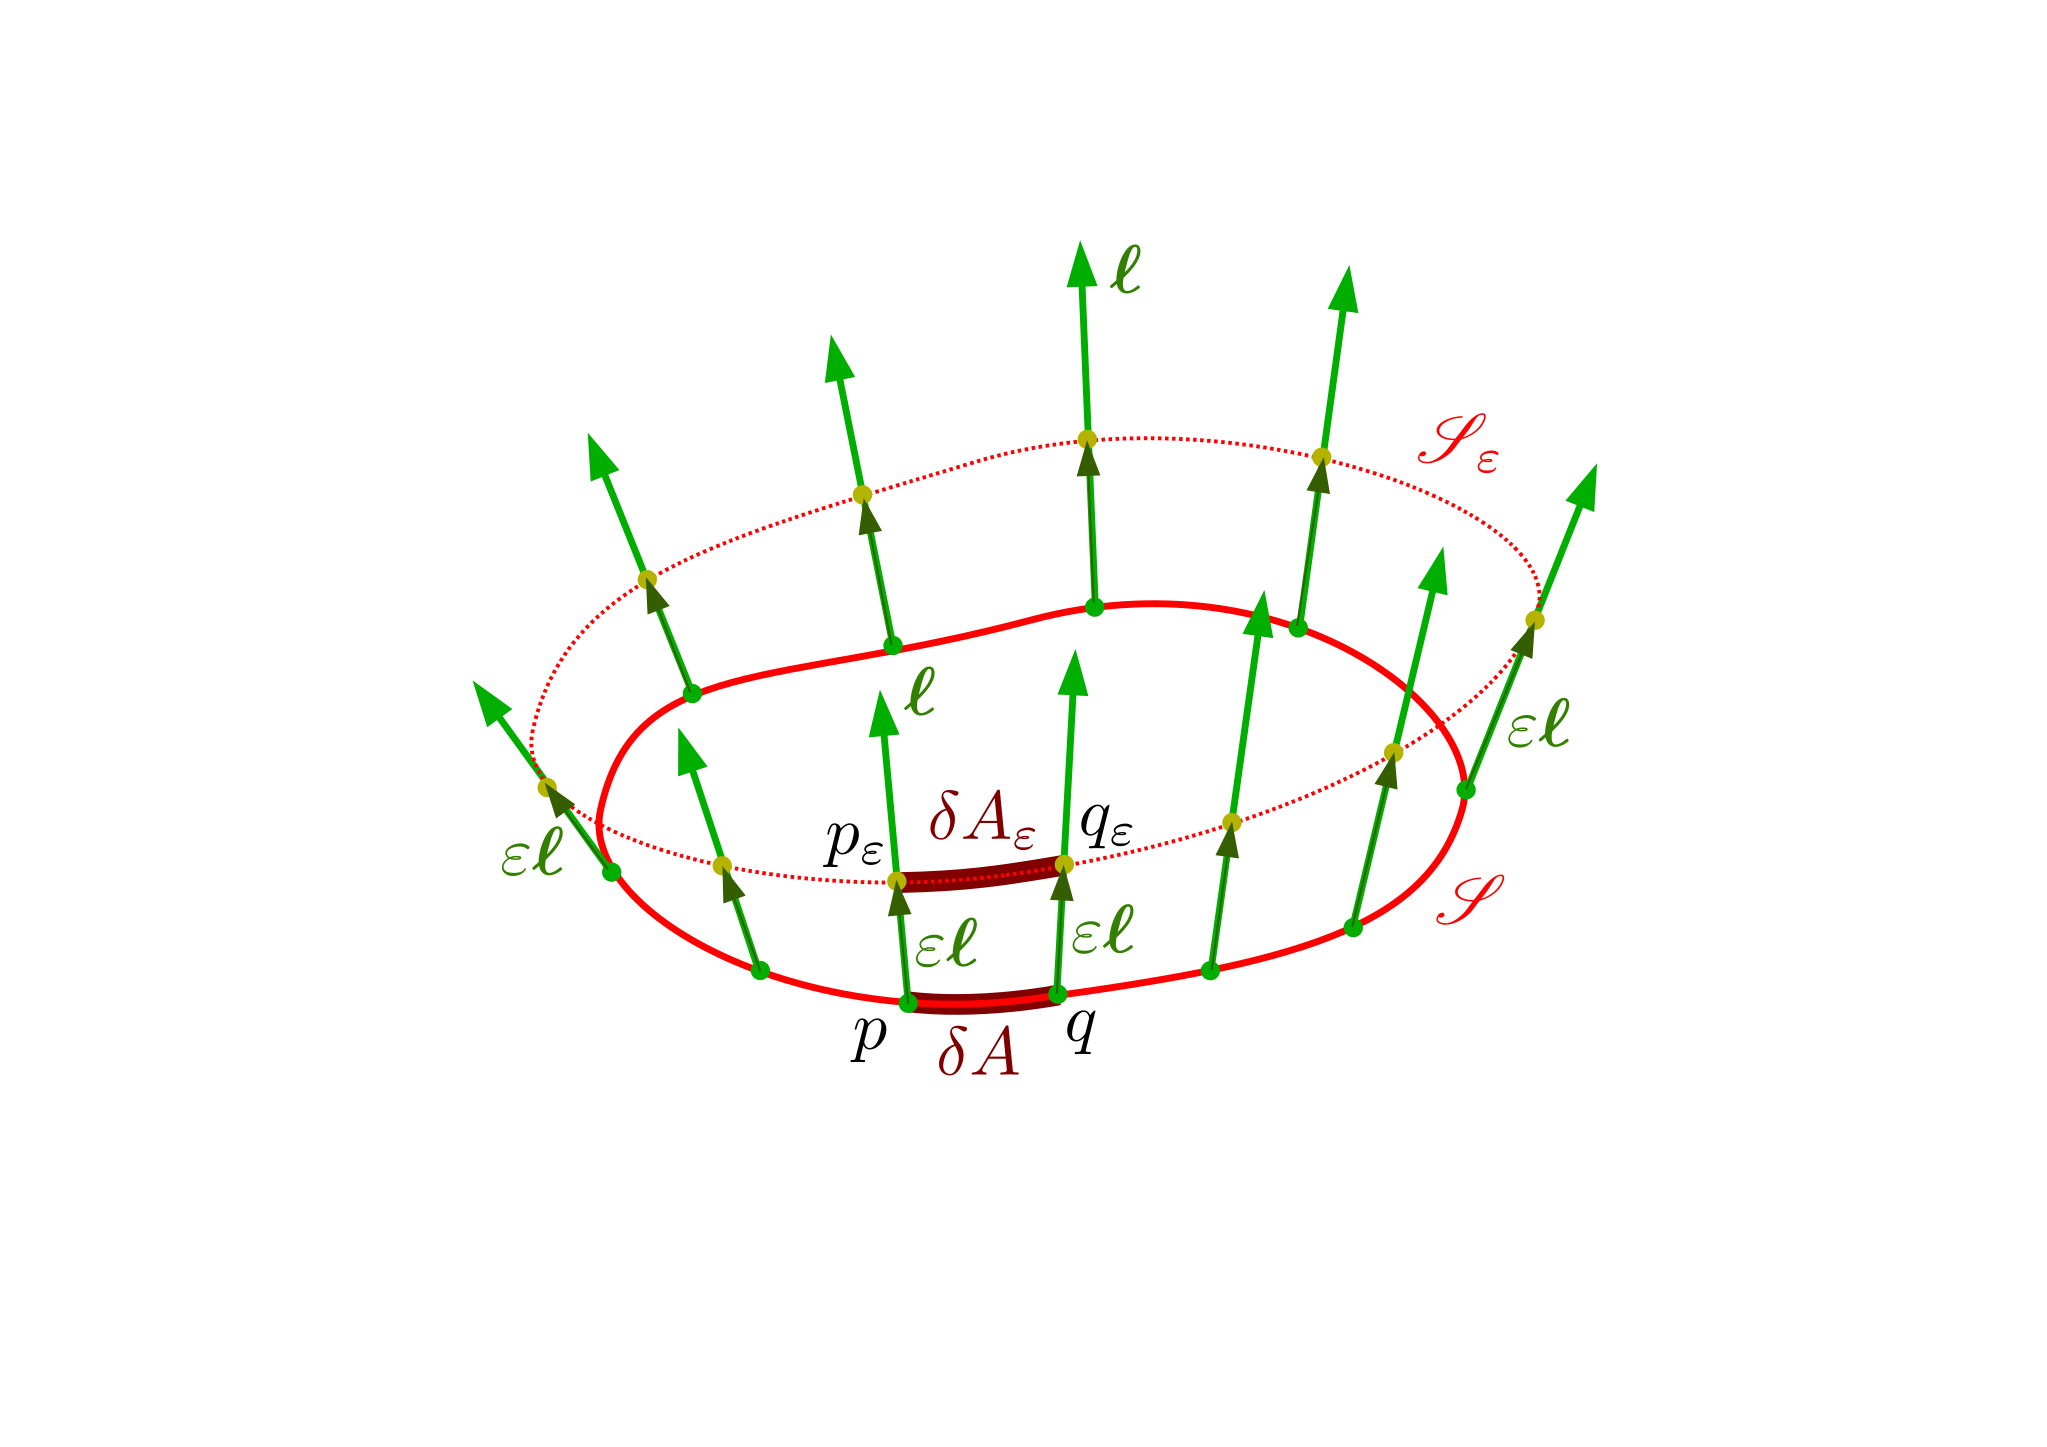
\includegraphics[width=0.6\textwidth]{def_expansion.pdf}}
\caption[]{\label{f:def:expansion} \footnotesize
Lie dragging of the surface $\Sp$ along $\wl$ by the small parameter $\varepsilon$.
$\Sp$ is drawn as a 1-dimensional submanifold, while it is actually a
$(n-2)$-dimensional one, $n$ being the spacetime dimension.}
\end{figure}

Let us define the expansion of the spacelike section $\Sp$ along the vector
field $\wl$ as follows. Given an infinitesimal parameter $\varepsilon\geq 0$, take a point
$p\in \Sp$ and displace it by the infinitesimal vector $\varepsilon \wl$, thereby getting
a nearby point $p_\varepsilon$ (cf. Fig.~\ref{f:def:expansion}).
Since $\wl$ is tangent to $\Hor$ and $p\in\Hor$, we have $p_\varepsilon\in\Hor$.
By repeating this for each point in $\Sp$,
keeping the value of $\varepsilon$ fixed, we define a new codimension-2 surface,
$\Sp_\varepsilon$ say cf. Fig.~\ref{f:def:expansion}). One says that $\Sp_\varepsilon$ is obtained
from $\Sp$ by \defin{Lie dragging along $\wl$ by the parameter $\varepsilon$}\index{Lie!dragging}.
Note that $\Sp_0 = \Sp$.
Since $p_\varepsilon\in\Hor$ for every $p\in\Sp$, we have $\Sp_\varepsilon\subset \Hor$.
Because the null direction $\wl$ is transverse to $\Sp_\varepsilon$ by construction, it
follows that $\Sp_\varepsilon$ is spacelilke (cf. the lemma in Sec.~??).

At each point $p\in\Sp$, the \defin{expansion of $\Sp$ along $\wl$} is defined from the
rate of change $\theta_{(\wl)}$ of the area $\delta A$ of an element of surface $\delta S$ of
$\Sp$ around $p$:
\be \label{e:def:def_expansion}
    \theta_{(\wl)} := \lim_{\varepsilon\rightarrow 0} \frac{1}{\varepsilon}
    \frac{\delta A_\varepsilon - \delta A}{\delta A} .
\ee
In the above formula, $\delta A_\varepsilon$ stands for the area of the
surface element $\delta S_\varepsilon\subset \Sp_\varepsilon$ that is obtained from $\delta S$ by
Lie dragging along $\wl$ by the parameter $\varepsilon$ (cf. Fig.~\ref{f:def:expansion}).
\begin{remark}
The reader may wonder why the expansion is not denoted by something like
$\theta_{(\wl)}(\Sp)$, since its definition depends explicitely on
$\Sp$. We shall below that, because $\Hor$ is a null hypersurface, $\theta_{(\wl)}$
is actually independent of the choice of the spacelike section $\Sp$.
\end{remark}


For concreteness, let us assume that the element of surface $\delta S \subset\Sp$ is a $(n-2)$-dimensional
parallelogram delimited by some infinitesimal displacement vectors
$\D\w{x}_{(2)},\ldots,\D\w{x}_{(n-1)}$. The area of $\delta S$ is then
\be \label{e:def:A_wepsS_dx}
    \delta A = \wepsS(\D\w{x}_{(2)},\ldots,\D\w{x}_{(n-1)}),
\ee
where $\wepsS$ is the Levi-Civita tensor\index{Levi-Civita!tensor}
associated with the metric $\w{q}$
in $\Sp$ (cf. Sec.~\ref{s:bas:Levi-Civita_tensor} in Appendix~\ref{s:bas}).
Since $\w{q}$ is the metric induced by $\w{g}$ in $\Sp$ and $(\w{n},\w{s})$
is an orthonormal basis of $T_p^\perp \Sp$, $\wepsS$ is actually the
alternating form induced on $\Sp$ by the spacetime Levi-Civita tensor
$\weps$:
\be \label{e:def:epsS_ns}
    \encadre{ \wepsS = \weps(\w{n},\w{s},\ldots) },
\ee
or, in index notation,
\[
    \epsS_{\alpha_1\cdots\alpha_{n-2}} = \eps_{\mu\nu\alpha_1\cdots\alpha_{n-2}} n^\mu s^\nu .
\]
\begin{proof}
To demonstrate (\ref{e:def:epsS_ns}), it sufficies to note that its right-hand side
defines a fully antisymmetric $(n-2)$-linear form on $T_p\Sp$. Since the space
of such forms is 1-dimensional (for $\dim T_p\Sp = n-2$), we have then
necessarily $\wepsS = a \weps$ for some proportionality factor $a$. Since
$\weps(\w{n},\w{s},\D\w{x}_{(2)},\ldots,\D\w{x}_{(n-1)})$ is the volume
of the $n$-parallelepiped construted on the vectors $\w{n},\w{s},\D\w{x}_{(2)},\ldots,\D\w{x}_{(n-1)}$ and $\w{n}$ and $\w{s}$ are unit-length vectors for the metric $\w{g}$,
we have
\[
    \weps(\w{n},\w{s},\D\w{x}_{(2)},\ldots,\D\w{x}_{(n-1)}) = \delta A.
\]
This implies that $a=1$, thereby establishing (\ref{e:def:epsS_ns}).
\end{proof}
An alternative expression of $\wepsS$ is obtained by substituting (\ref{e:def:ns_lk})
for $\w{n}$ and $\w{s}$ in (\ref{e:def:epsS_ns}). Thanks to the multilinearity
and antisymmetry of $\weps$, we get
\be
    \encadre{ \wepsS = \weps(\w{k},\wl,\ldots) } .
\ee

Let us consider in some vicinity of $\Sp$ a coordinate system
\[
    x^\alpha = \left(\varepsilon, u, x^2,\ldots, x^{n-1}\right)
\]
that is adapted to $\Sp$ and $\wl$ in the sense that
\be \label{e:def:l_dsdeps}
    \wl = \der{}{\varepsilon}
\ee
and the points of $\Sp$ are defined by $(\varepsilon,u) = (0,0)$.
Then, from the very definition of the Lie dragging of $\Sp$ along $\wl$, we
have
\be
    \Sp_\varepsilon = \left\{ p\in\M,\quad  (x^0(p), x^1(p)) = (\varepsilon,0)
                        \right\}
\ee
and  $x^a = (x^2,\ldots, x^{n-1})$ can  be viewed as a coordinate system\footnote{
Latin indices from the beginning of the alphabet, $a$, $b$, etc. range from $2$
to $n-1$.} on each surface $\Sp_\varepsilon$.
Let us choose the $n-2$ infinitesimal displacement vectors in (\ref{e:def:A_wepsS_dx})
along the coordinate lines of this system:
\be
    \D x_{(i)}^a = (\underbrace{0,\ldots,0}_{i-2},\D x^i,
                    \underbrace{0,\ldots,0}_{n-1-i}), \qquad
                    2\leq i \leq n-1 .
\ee
Then expression~(\ref{e:def:A_wepsS_dx}) for the area of $\delta S$ becomes
\bea
    \delta A & = & \epsS_{a_1 \cdots a_{n-2}} \, \D x_{(2)}^{a_1} \cdots \D x_{(n-1)}^{a_{n-2}}
                    \nonumber \\
            & = & \epsS_{2\cdots(n-1)} \, \D x^2 \cdots \D x^{n-1} \nonumber \\
     \delta A  & = & \sqrt{q} \, \D x^2 \cdots \D x^{n-1} , \label{e:def:A_sqrt_q}
\eea
where we have used (\ref{e:bas:eps_sqrt_g}) for the components of the
Levi-Civita tensor $\wepsS$, $q$ standing for the determinant of the metric
$\w{q}$ with respect to the coordinates $(x^2,\ldots,x^{n-1})$.
By the very definition of the Lie dragging, the surface element
$\delta S_\varepsilon$ on $\Sp_\varepsilon$
is defined by the same values of the coordinates $(x^2,\ldots, x^{n-1})$
as $\Sp$. In particular, the small coordinate increments $\D x^2$, ..., $\D x^{n-1}$
take the same values as on $\Sp$. Therefore, the area of $\delta S_\varepsilon$
is
\be \label{e:def:A_eps_sqrt_q}
    \delta A_\varepsilon = \sqrt{q(\varepsilon)} \, \D x^2 \cdots \D x^{n-1} ,
\ee
where $q(\varepsilon)$ stands for the determinant of the components of the
metric $\w{q}(\varepsilon)$ induced by $\w{g}$ on $\Sp_\varepsilon$. Since
$\Sp_\varepsilon$ is spacelike (cf. above), $\w{q}(\varepsilon)$ is positive definite, so
that $q(\varepsilon)\geq 0$.

In view of (\ref{e:def:A_sqrt_q})-(\ref{e:def:A_eps_sqrt_q}), the definition (\ref{e:def:def_expansion})
of the expansion of $\Sp$ along $\wl$ can be rewritten as
\[
    \theta_{(\wl)} = \lim_{\varepsilon\rightarrow 0} \frac{1}{\varepsilon}
    \frac{\sqrt{q(\varepsilon)} - \sqrt{q(0)}}{\sqrt{q(0)}} .
\]
We recognize the derivative of the function $\varepsilon \mapsto \ln \sqrt{q(\varepsilon)}=
1/2\, \ln q(\varepsilon)$ at $\varepsilon=0$:
\be
     \theta_{(\wl)} = \frac{1}{2} \frac{\D}{\D\varepsilon}  \ln q .
\ee
Given that $\Sp_\varepsilon$ is deduced from $\Sp$ by a Lie dragging along $\wl$
and $\varepsilon$ is the parameter associated with $\wl$ [cf. Eq.~(\ref{e:def:l_dsdeps})], we may
rewrite this formula as the Lie derivative of $\ln q$ along $\wl$:
\be
    \theta_{(\wl)} = \frac{1}{2} \Lie{\el} \ln q .
\ee
Using the general law of variation of a derminant, as given by Eq.~(\ref{e:bas:variation_det})
in Appendix~\ref{s:bas}, we may write
\[
    \theta_{(\wl)} = \frac{1}{2} \, \mathrm{tr} \left(Q^{-1} \times \Lie{\el} Q \right) ,
\]
when $Q$ is the matrix representing the components of $\w{q}$ with respect to the
coordinates $(x^a) = (x^2,\ldots, x^{n-1})$. In index notation, we have
$Q = (q_{ab})$ and $Q^{-1} = (q^{ab})$. Hence
\be
    \theta_{(\wl)} = \frac{1}{2} \, q^{ab} \Liec{\el} q_{ab} .
\ee
We may wonder about the link between the Lie derivative along $\wl$ of the $(n-2)$-metric
$\w{q}$ of the spacelike sections $\Sp_\varepsilon$, which appears above, and
the Lie derivative along $\wl$ of the spacetime extension $\w{q}$ defined by
(\ref{e:def:q_g_k_l}). For the sake of clarity, let us denote here the latter
by $\w{\bar q}$. More precisely, we may consider that $\w{\bar q}$ is a
field defined in some neighbourhood of the portion of $\Hor$ sliced by
$\bigcup_{\varepsilon} \Sp_\varepsilon$ via (\ref{e:def:q_g_k_l}), with $\w{k}$
defined at each point $p\in\Sp_\varepsilon$ as the unique null vector of
$T_p^\perp\Sp_\varepsilon$ obeying $\wl\cdot\w{k}=-1$.
Let $(\w{u},\w{v})$ be a pair of vector fields on $\Hor$, which are tangent
to the spacelike sections $\Sp_\varepsilon$. The Leibniz rule implies
\[
     \Lie{\el} \w{\bar q} \,
\]
  % The concept of black hole 1: Horizons as null hypersurfaces

\chapter{The concept of black hole 2: Non-expanding horizons}
\label{s:neh}

\minitoc

\section{Introduction}

Having discussed in depth the geometry of null hypersurfaces in Chap.~\ref{s:def}
we move forward here to distinguish a null hypersurface representing a black hole event horizon from, let us say, a future light cone. We do it for black holes
\emph{in equilibrium}. Indeed, for such black holes, it is quite natural
to assume a vanishing expansion. This leads us the concept of \emph{non-expanding
horizon} (Sec.~\ref{s:neh:neh}). A special kind of these objects is that
of \emph{Killing horizons} (Sec.~\ref{s:neh:Killing_hor}). Actually, we shall
see in Chap.~\ref{s:sta} that the event horizon of a black hole in equilibrium
must be a Killing horizon.


%%%%%%%%%%%%%%%%%%%%%%%%%%%%%%%%%%%%%%%%%%%%%%%%%%%%%%%%%%%%%%%%%%%%%%%%%%%%%%%%%%%%%%%%

\section{Non-expanding horizons} \label{s:neh:neh}

\subsection{Motivation and definition}

Having discussed in depth the geometry of null hypersurfaces, and in particular
their expansion, let us make an attempt to distinguish a black hole event
horizon from, let us say, a future light cone.
To get the localized behaviour mentioned in the black hole naive definition
of Sec.~\ref{s:def:first_defin}, we could demand that the area of the
spacelike cross-sections remains constant, in other words that
the expansion along the null normal vanishes. Hence the definition:\\
A \defin{non-expanding horizon}\index{non-expanding!horizon}\index{horizon!non-expanding --} is a null hypersurface $\Hor$ having the
topology (\ref{e:def:H_topology}):
\be
    \Hor \simeq \R \times \Sp,
\ee
where $\Sp$ is a closed manifold of dimension $n-2$,
and such that the expansion of $\Hor$ along any null normal $\wl$ vanishes
identically:
\be
    \theta_{(\wl)} = 0 .
\ee
Note that, given the scaling law (\ref{e:def:rescale_lambda}),
if $\theta_{(\wl)} = 0$ for some normal $\wl$, then  $\theta_{(\wl')} = 0$
for any other normal $\wl'$. Hence the definition of a non-expanding horizon
does not depend on the choice of the null normal.

As we shall discuss in detail in Chap.~\ref{s:sta}, this definition captures only
the event horizon of black holes in equilibrium.

\begin{example}[Schwarzschild horizon]
In view of Eq.~(\ref{e:def:theta_Schw_hor}), we may assert that the
Schwarz\-schild horizon considered in Examples~\ref{x:def:Schw_hor}, \ref{x:def:Schw_hor2},
\ref{x:def:Schw_hor3}, \ref{x:def:Schw_hor4}, \ref{x:def:Schw_hor5}, \ref{x:def:Schw_hor6},
\ref{x:def:Schw_hor7}, \ref{x:def:Schw_hor8} and \ref{x:def:Schw_hor9}
of Chap.~\ref{s:def}
is a non-expanding horizon.
\end{example}

\begin{hist}\label{h:neh:NEH}
The concept of non-expanding horizon has been introduced by P.~H\'a\'\j i\v{c}ek
in 1973 under the name of \emph{totally geodesic null hypersurface} \cite{Hajic73a}
or \emph{perfect horizon} \cite{Hajic73b,Hajic74}.
The terminology \emph{non-expanding horizon} is due to A.~Ashtekar, S.~Fairhurst
and B.~Krishnan in 2000 \cite{AshteFK00} (see also \cite{AshteBL02}).
\end{hist}

\subsection{Invariance of the area}

Given a cross-section $\Sp$ of $\Hor$, the area\index{area!of a cross-section} of $\Sp$, with respect to the spacetime metric $\w{g}$, is [cf. Eqs.~(\ref{e:def:A_wepsS_dx}) and (\ref{e:def:A_sqrt_q})]
\be \label{e:neh:total_area}
    A = \int_{\Sp} \wepsS(\D\w{x}_{(2)},\ldots,\D\w{x}_{(n-1)})
        = \int_{\Sp} \sqrt{q} \, \D x^2 \cdots \D x^{n-1} ,
\ee
where $x^a = (x^2, \ldots, x^{n-1})$ is a coordinate system on $\Sp$ and $q$ is
the determinant with respect to these coordinates of the Riemannian metric $\w{q}$
induced by $\w{g}$ on $\Sp$.

A direct consequence of the definition of a non-expanding horizon is that
$A$ does not depend on the choice of the cross-section $\Sp$.
\begin{proof}
Let $\Sp'$ be a second cross-section of $\Hor$ and let $\wl$ be a field of null normals
of $\Hor$. Along the null geodesic generators of $\Hor$, we can always choose a parameter $\lambda$ associated with $\wl$ (i.e. such that $\wl = \D/\D\lambda$ along a given null geodesic generator)
such that $\lambda=0$ on $\Sp$. By the very definition of a cross-section,
any null geodesic generator $\Li$ of $\Hor$ intersects $\Sp'$ at a single point. Let
$\lambda_0$ be the value of $\lambda$ at this point. We may then introduce
a new parameter along $\Li$ as follows:
\[
      \lambda' = \frac{\lambda}{\lambda_0} .
\]
If we repeat this for all null geodesic generators of $\Hor$, we obtain a parametrization
of all the null geodesic generators that satisfies $\lambda'=0$ on $\Sp$ and $\lambda'=1$
on $\Sp'$. Let $\wl'=\D/\D\lambda'$ be the (null) tangent vector associated
with $\lambda'$. We may then say that the cross-section $\Sp'$ is deduced
from $\Sp$ by the Lie dragging of $\Sp$ along $\wl'$ by a parameter $\delta\lambda'=1$.
More precisely, we may considered that $\Sp'$ is deduced from $\Sp$ by a
continuous deformation, represented by a 1-parameter family $(\Sp_{\lambda'})$
of cross-sections such that $\Sp_0 = \Sp$ and $\Sp_1 = \Sp'$. Associated
with this family is a real-valued function $\lambda' \mapsto A(\lambda')$
given the area of each element $\Sp_{\lambda'}$. By the very definition
of the expansion along $\wl'$ [Eq.~(\ref{e:def:def_expansion})], we have then
\[
    \frac{\D A}{\D\lambda'} = \int_{\Sp_{\lambda'}} \theta_{(\wl')} \, \delta A .
\]
If $\Hor$ is a non-expanding horizon, then $\theta_{(\wl')}=0$ and it follows
that $A(\lambda')$ is a constant function. Hence the area of $\Sp'$ is equal
to that of $\Sp$.
\end{proof}
Given that the quantity $A$ defined by (\ref{e:neh:total_area})
takes a unique value whatever the cross-section $\Sp$,
we call it the \defin{area of the non-expanding horizon}\index{area!of a non-expanding horizon}
$\Hor$.

\begin{example}[Schwarzschild horizon]
The area of the Schwarzschild horizon is readily computed from
the metric (\ref{e:def:q_S_Schw_hor}):
$q_{ab} \D x^a \D x^b = 4m^2 \left( \D\th^2 + \sin^2\th \D^2\ph \right)$;
we get
\[
     A = 16\pi m^2 .
\]
\end{example}

\subsection{Trapped surfaces}

If there is a natural concept of \emph{outer}/\emph{inner} for $\Hor$, for
instance the outer region being the one that contains an asymptotically flat end,
and if the transverse null normals $\w{k}$ point to the inner region, then
the property $\theta_{(\wl)}=0$ means that any cross-section $\Sp$ of the
non-expanding horizon $\Hor$ is a
\defin{marginally outer trapped surface}\index{marginally!outer trapped surface}\index{trapped!surface!marginally outer --}
(often abridged as \defin{MOTS}\index{MOTS}). This definition is due to
Hawking \cite{Hawki73}, an
\defin{outer trapped surface}\index{outer!trapped surface}\index{trapped!surface!outer --}
would be one for which $\theta_{(\wl)}\leq 0$.

\begin{figure}
\vspace{5cm}
%\centerline{\includegraphics[width=0.6\textwidth]{}}
\caption[]{\label{f:neh:expansions_flat} \footnotesize
Inward and outward expansions of a closed spacelike surface in Minkowski
spacetime.}
\end{figure}


This definition is related to, but distinct from, the definition of a
marginally trapped surface by Penrose \cite{Penro65}: a $(n-2)$-dimensional
submanifold $\Sp$ of $\M$ is a \defin{trapped surface}\index{trapped!surface}
 iff (i) $\Sp$ is
closed (i.e. compact without boundary), (ii) $\Sp$ is spacelike and (iii)
the two systems of null geodesics emerging orthogonally from $\Sp$ converge
locally at $\Sp$, i.e. they have negative expansions:
\be
    \theta_{(\wl)} < 0 \quad\mbox{and}\quad \theta_{(\w{k})} < 0 ,
\ee
where the expansion along $\w{k}$ is defined in the same way as that along
$\wl$ [cf. Eq.~(\ref{e:def:theta_l_all})]:
\be
    \theta_{(\w{k})} := \lim_{\varepsilon\rightarrow 0} \frac{1}{\varepsilon}
    \frac{\delta A^{(\w{k})}_\varepsilon - \delta A}{\delta A}
        = \frac{1}{2} \Lie{\w{k}} \ln q
        = \frac{1}{2} \, q^{\mu\nu} \Liec{k} q_{\mu\nu}
        = q^{\mu\nu} \nabla_\mu k_\nu ,
\ee
$\delta A^{(\w{k})}_\varepsilon$ begin the area of the surface element
that is deduced from the surface element of area $\delta A$ on $\Sp$ by the
Lie dragging along $\w{k}$ by a parameter $\varepsilon$.
The limit case $\theta_{(\wl)} = 0$ and $\theta_{(\w{k})}<0$ correspond
to the so-called \defin{marginally trapped surface}\index{marginally!trapped!surface}.

In a flat spacetime (Minkowski), given any spacelike surface,
one has $\theta_{(\wl)} > 0$ and $\theta_{(\w{k})} < 0$ (cf. Fig.~\ref{f:neh:expansions_flat}), so there
is no trapped surface.

Cross-sections of a non-expanding horizon are usually marginally trapped surfaces
(cf. the example below).
However there exist some pathological situations for
which $\theta_{(\w{k})} > 0$ at some points of $\Sp$ \cite{GerocH82}.

\begin{example}
Let us consider a cross-section $\Sp$ of the Schwarzschild horizon as
defined in Example~\ref{x:def:Schw_hor4} of Chap.~\ref{s:def}.
Computing $q^{\mu\nu} \nabla_\mu k_\nu$ from the components $k_\nu$
given by (\ref{e:def:l_k_forms_Schw_hor}) we get (cf. Appendix~\ref{s:sam})
\[
    \theta_{(\w{k})} = - \frac{r+2m}{r^2} .
\]
In particular, on $\Sp$ ($r=2m$),
\[
    \theta_{(\w{k})}  = - \frac{1}{m} .
\]
Hence $\theta_{(\w{k})} < 0$. Since we had already $\theta_{(\wl)}=0$
[cf. Eq.~(\ref{e:def:theta_Schw_hor})], we conclude that $\Sp$ is a
marginally trapped surface. This could also have been inferred from
Fig.~\ref{f:def:Schw_hor_lk}, since according to the metric
(\ref{e:def:q_Schw_hor}), the area of the cross-sections of $\Hor$
is nothing but $4\pi r^2$ and $\w{k}$ points to decreasing values of $r$, while, on $\Hor$,
$\wl$ points to a fixed value of $r$.
\end{example}

\subsection{Vanishing of the deformation rate tensor} \label{s:neh:NEH_Theta_zero}

If $\Hor$ is a non-expanding horizon, we may set $\theta_{(\wl)}=0$
in the null Raychaudhuri equation (\ref{e:def:null_Raychaud}); it reduces then
to
\be \label{e:neh:null_Raychaud_theta_zero}
    \sigma_{ab} \sigma^{ab} + 8\pi \w{T}(\wl, \wl) = 0 .
\ee
The first term is always non-negative:
\be \label{e:neh:sigma_square}
    \sigma_{ab} \sigma^{ab} \geq 0 .
\ee
\begin{proof}
Since $\w{\sigma}$ is symmetric, it can be diagonalized
in an orthonormal basis of $\w{q}$: $\sigma_{ab} = \mathrm{diag}(s_1,\ldots, s_{n-2})$.
Moreover, $\w{q}$ being a Riemannian metric, we have, in the same basis, $q^{ab} = \mathrm{diag}(1,\ldots,1)$. Since $\sigma^{ab} = q^{am} q^{bn} \sigma_{mn}$, we conclude that
\be \label{e:neh:sigma_square_si}
  \sigma_{ab} \sigma^{ab} = s_1^2 + \cdots + s_{n-2}^2 \geq 0 .
\ee
\end{proof}

Regarding the second term in (\ref{e:neh:null_Raychaud_theta_zero}), it
is quite natural to assume that matter and non-gravitational fields,
represented by the total energy-momentum tensor $\w{T}$, obey the
\defin{null energy condition}\index{null!energy condition}\index{energy!condition!null --},
namely that
\be \label{e:neh:null_energy_cond}
    \w{T}(\wl, \wl) \geq 0 \quad \mbox{for any null vector $\wl$}.
\ee
This condition is pretty weak and is satisfied by
\begin{itemize}
\item vacuum: $\w{T}=0$;
\item any ``reasonable'' matter model, such as a perfect fluid with a
proper energy density $\varepsilon$ and pressure $p$ satisfying
$\varepsilon+p\geq 0$;
\item any electromagnetic field;
\item any real or complex scalar field;
\item ``dark energy''\index{dark energy} modelled by $\w{T} = -\frac{\Lambda}{8\pi}\, \w{g}$.
\end{itemize}
Note also that the null energy condition is implied by the
so-called \defin{weak energy condition}\index{weak!energy condition}\index{energy!condition!weak --},
which states that
\be
    \w{T}(\w{u}, \w{u}) \geq 0 \quad \mbox{for any timelike vector $\w{u}$}.
\ee
The null energy condition follows from the
weak energy condition by continuity.
Selecting for $\w{u}$ the 4-velocity of an observer, we see that
the weak energy condition has a simple physical interpretation: the energy
density as measured by any observer is non-negative.

Given (\ref{e:neh:sigma_square}) and (\ref{e:neh:null_energy_cond}),
Eq.~(\ref{e:neh:null_Raychaud_theta_zero})  implies both
\be
    \sigma_{ab} \sigma^{ab}  = 0
\ee
and
\be \label{e:neh:T_l_l_zero}
    \w{T}(\wl, \wl) = 0 .
\ee
The identity $\sigma_{ab} \sigma^{ab} = 0$ is possible only if each of
the $s_i$'s in (\ref{e:neh:sigma_square_si}) is zero. Hence we have necessarily
\be
    \w{\sigma} = 0 .
\ee
Since we had already $\theta_{(\wl)}=0$ (non-expanding horizon), this implies that the full deformation rate tensor
vanishes identically [cf. Eq.~(\ref{e:def:def_shear})]:
\be
    \w{\Theta} = 0 .
\ee
In view of (\ref{e:def:Theta}), this is equivalent to
\be \label{e:neh:Lie_el_q_zero}
     \vw{q}^* \Lie{\el} \w{q} = 0 .
\ee
We conclude that, provided that the null energy condition holds,
the whole metric (and not only the area element
$\wepsS$, as a mere $\theta_{(\wl)}=0$ would suggest) of any cross-section
of a non-expanding horizon is invariant along the null geodesic generators.

\begin{example}[Schwarzschild horizon]
We had already noticed that, for the Schwarzschild horizon, $\w{\Theta}=0$
[Eq.~(\ref{e:def:Theta_zero_Schw_hor}) in Example~\ref{x:def:Schw_hor8}
of Chap.~\ref{s:def}].
\end{example}

\subsection{Induced affine connection}

Since $\Hor$ is a null hypersurface, the ``metric'' $\left. \w{g}\right|_{\Hor}$
induced on it by the spacetime metric $\w{g}$ is degenerate. As a consequence, there
is a priori no unique connection on $\Hor$ associated with it. However, when
$\Hor$ is a non-expanding horizon and the null energy condition holds on $\Hor$,
so that $\w{\Theta}=0$, the spacetime connection $\wnab$ induces a unique
connection ${}^\Hor\!\wnab$ on $\Hor$ as follows.
Let $\w{u}$ and $\w{v}$ be two vector fields on $\Hor$. We have, using
(\ref{e:def:nab_l_Theta}) to express $\nabla_\nu \el_\mu$ in terms of $\Theta_{\nu\mu}$:
\bea
    \el_\mu u^\nu \nabla_\nu v^\mu &= &
        u^\nu \nabla_\nu ( \underbrace{\el_\mu v^\mu}_{0} )
        - v^\mu u^\nu \nabla_\nu \el_\mu \nonumber \\
        & = & - \underbrace{\Theta_{\nu\mu}}_{0} v^\mu u^\nu  - \omega_\nu u^\nu
            \underbrace{\el_\mu v^\mu}_{0}
            + v^\mu \underbrace{u^\nu \el_\nu}_{0} k^\sigma\nabla_\sigma \el_\mu
             = 0    \nonumber .
\eea
Hence $\wl$ is orthogonal to the vector field $\wnab_{\w{u}} \w{v}$. It follows
immediately that $\wnab_{\w{u}} \w{v}$ is tangent to $\Hor$.
We conclude that the operator
\be
    \begin{array}{cccc}
    {}^\Hor\!\wnab \ : & \mathscr{X}(\Hor)\times\mathscr{X}(\Hor) & \longrightarrow & \mathscr{X}(\Hor) \\
    & (\w{u},\w{v}) & \longmapsto & \wnab_{\w{u}} \,\w{v} ,
    \end{array}
\ee
where $\mathscr{X}(\Hor)$ is the space of vector fields on $\Hor$, is
well defined (i.e. ${}^\Hor\!\wnab_{\w{u}}\w{v}$  does belong to
$\mathscr{X}(\Hor)$).
Moreover this operator fulfills all the properties of an affine connection
(cf. Sec.~\ref{s:bas:affine_connect}), since $\wnab$ does.
We naturally call ${}^\Hor\!\wnab$ the \defin{affine connection induced on $\Hor$
by}\index{induced! affine connection}\index{affine connection!induced --}\index{connection!induced --} $\wnab$.

A geometrical consequence of the identity
${}^\Hor\!\wnab_{\w{u}}\w{v} = \wnab_{\w{u}}\w{v}$ is
that $(\Hor, {}^\Hor\!\wnab)$ is a \defin{totally geodesic submanifold}\index{totally geodesic} of $(\M,\w{g})$:
i.e. any geodesic of $(\Hor, {}^\Hor\!\wnab)$ is also a geodesic of $(\M,\w{g})$
(cf. the historical note on page~\pageref{h:neh:NEH}).


\subsection{Going further}

See Refs.~\cite{AshteK04,GourgJ06,Jaram13} for more
about non-expanding horizons, in particular for a subclass of them
called \emph{isolated horizons}\index{isolated!horizon}\index{horizon!isolated}.


%%%%%%%%%%%%%%%%%%%%%%%%%%%%%%%%%%%%%%%%%%%%%%%%%%%%%%%%%%%%%%%%%%%%%%%%%%%%%%%

\section{Killing horizons} \label{s:neh:Killing_hor}

A special kind of non-expanding horizons, which is of primordial
importance for the theory of
stationary black holes, is that of Killing horizons with closed-manifold cross-sections.
Defining a Killing horizon requires the concepts of 1-dimensional group of
isometries and Killing vector, which we discuss first.

\begin{figure}
\centerline{\includegraphics[width=0.8\textwidth]{def_group_action.pdf}}
\caption[]{\label{f:neh:group_action} \footnotesize
Group action of $G$ on $\M$.}
\end{figure}


\subsection{Spacetime symmetries} \label{s:neh:symmetries}

Symmetries of spacetime are described in a coordinate-independent way by means of
a (symmetry) group acting on the spacetime manifold $\M$.
Through this action, each transformation belonging to the group displaces points within $\M$ and one demands that the metric $\w{g}$ is invariant under such displacement.
More precisely, given
a group $G$, a \defin{group action}\index{group!action} of $G$ on $\M$ is a map\footnote{Do no confuse the generic element $g$ of the group $G$ with the metric tensor $\w{g}$.}
\be
	\begin{array}{rccl}
	\Phi: & G\times \M & \longrightarrow & \M \\
		& (g,p) & \longmapsto & \Phi(g,p) =: \Phi_g(p)
	\end{array}
\ee
such that (cf. Fig.~\ref{f:neh:group_action})
\begin{itemize}
\item if $e$ is the identity element of $G$, then
$\forall p\in \M,\  \Phi_e(p) = p$ ;
\item $\forall (g,h) \in G^2,\  \forall p\in\M,\  \Phi_g(\Phi_h(p)) = \Phi_{gh}(p)$, where $gh$ stands for the product of $g$ by $h$ according to the group law of
$G$.
\end{itemize}
The \defin{orbit}\index{orbit!under a group action} of a point $p\in\M$ is the set $\{g(p),\ g\in G\}\subset\M$, i.e. the set of points which are connected to $p$ by some group transformation. One says that $p$ is a
\defin{fixed point}\index{fixed!point} of the group action if its orbit is
reduced to $\{p\}$.

An important class of group actions are those for which $G$ is a 1-dimensional
\emph{Lie group}, i.e. a ``continuous'' group (actually a ``differentiable'' group).
Then around $e$, the elements of $G$ can be labelled by a parameter $t\in \R$, such that $g_{t=0} = e$. It is then
common to use the shorthand notation
\be
        \Phi_t := \Phi_{g_t} .
\ee
Because $G$ is a 1-dimensional Lie group, the orbit of a given point $p\in\M$ under the group action is then either $\{p\}$ (when $p$ is fixed point of the
group action) or a curve of $\M$. In the latter case,
$t$ is a natural parameter along the curve (cf. Fig.~\ref{f:neh:orbit_group}). The tangent vector corresponding to that parameter is called the \defin{generator of the group} $G$
(associated with the $t$-parametrization). At each point $p$ of
an orbit, it is given by
\be \label{e:neh:xi_dxdt}
    \w{\xi} = \frac{\D\w{x}}{\D t} ,
\ee
where $\D\w{x}$ is the infinitesimal vector connecting the point $p$ to the point
$\Phi_{\D t}(p)$ (cf. Sec.~\ref{s:bas:vectors} and Fig.~\ref{f:neh:orbit_group}).
We have then
\begin{greybox}
The action of $G$ on $\M$ limited to infinitesimal transformations of parameter
$\D t$ around the identity ($\D t =0$) amounts to translations along the infinitesimal vector $\D t\, \w{\xi}$.
\end{greybox}

\begin{figure}
\centerline{\includegraphics[height=0.25\textheight]{def_orbit_group.pdf}}
\caption[]{\label{f:neh:orbit_group} \footnotesize
Orbit of a point $p$ under the action $\Phi$ of a 1-dimensional Lie group, parametrized
by $t\in\R$. The vector $\w{\xi} = \D\w{x}/\D t$ is the group
generator associated with this parameter.}
\end{figure}

A 1-dimensional Lie group $G$ is said to be a
\defin{symmetry group}\index{symmetry!group}\index{group!symmetry --}
of the spacetime $(\M,\w{g})$ if there is an action $\Phi$ of $G$ on $\M$
such that for any value of the parameter $t$ of $G$,
$\Phi_t$ is an \defin{isometry}\index{isometry} of $(\M,\w{g})$, i.e. $\Phi_t$
preserves the ``distances'' and more generally the ``scalar products'' on
$(\M,\w{g})$, in the following sense: for any $p\in\M$ and any pair of points $(q,r)$
infinitely close to $p$, we shall have
\be \label{e:neh:isometry_dx}
    \left.\w{g}\right| _{\Phi_t(p)}(\D\w{x}', \D\w{y}') =
        \left.\w{g}\right| _{p}(\D\w{x}, \D\w{y}) ,
\ee
with the infinitesimal displacement vectors $\D\w{x} := \vp{pq}$, $\D\w{y} := \vp{pr}$,
$\D\w{x}' := \vp{\Phi_t(p)\Phi_t(q)}$ and $\D\w{y}' := \vp{\Phi_t(p)\Phi_t(r)}$
(cf. Sect.~\ref{s:fra:spacetime}).
Now, by definition, $\D\w{x}'$ is nothing but the pushforward
of the vector $\D\w{x}\in T_p\M$ to the tangent space
$T_{\Phi_t(p)}\M$ by the map $\Phi_t$
(cf. Sec.~\ref{s:bas:Lie_der_vector} in Appendix~\ref{s:bas}),
and similarly $\D\w{y}'$ is the pushforward of $\D\w{y}$ by $\Phi_t$:
\[
    \D\w{x}' = \Phi_t^*(\D\w{x}) \quad\mbox{and}\quad
    \D\w{y}' = \Phi_t^*(\D\w{y}) .
\]
By rescaling by infinitely small parameters (using the bilinearity of $\w{g}$),
it is clear that (\ref{e:neh:isometry_dx})
holds for finite vectors as well, so that we may say that $\Phi_t$ is an
isometry of $(\M,\w{g})$ iff
\be \label{e:neh:isometry}
    \forall p\in\M,\  \forall (\w{u},\w{v}) \in (T_p\M)^2,\quad
    \left. \w{g}\right| _{\Phi_t(p)} \left(\Phi_t^*(\w{u}), \Phi_t^*(\w{v})\right) =
    \left. \w{g}\right| _{p} (\w{u},\w{v}) ,
\ee
where $\Phi_t^*(\w{u})$ (resp. $\Phi_t^*(\w{v})$) is the pushforward of the vector $\w{u}\in T_p\M$ (resp. $\w{v}\in T_p\M$)
to the tangent space $T_{\Phi_t(p)}\M$ by $\Phi_t$ [cf. Eq.~(\ref{e:bas:def_Phi_eps})].
Given the definition (\ref{e:bas:def_pullback}) of the pullback of
a bilinear form, we may reexpress the isometry condition (\ref{e:neh:isometry})
in terms of the
pullback of $\w{g}$ by $\Phi_t$:
\be \label{e:neh:isometry_pullback}
    \Phi_t^*\w{g} = \w{g} .
\ee
Now, according the definition (\ref{e:bas:def_Lie_der_covar}) of the Lie
derivative, we have
\be
    \Lie{\xi} \w{g} := \lim_{t \rightarrow 0} \frac{1}{t}
    \left( \Phi_\varepsilon^*\w{g} - \w{g} \right) .
\ee
If $G$ is a symmetry group of $(\M,\w{g})$ with generator $\w{\xi}$,
(\ref{e:neh:isometry_pullback}) leads then to
$\Lie{\xi}\w{g} = 0$. The reverse is true by integration. Hence
we conclude:
\begin{greybox}
A 1-dimensional Lie group $G$
is a symmetry group of the spacetime $(\M,\w{g})$ iff the Lie derivative
of the metric tensor along the generator $\w{\xi}$ of $G$
vanishes identically:
\be \label{e:neh:Lie_xi_g}
    \encadre{\Lie{\xi}\w{g} = 0 } .
\ee
The vector field $\w{\xi}$ is then called a \defin{Killing vector}\index{Killing!vector field}
of $(\M,\w{g})$.
\end{greybox}
Expressing the Lie derivative via Eq.~(\ref{e:bas:Lie_der_comp_nab}) of Appendix~\ref{s:bas},
we see immediately that Eq.~(\ref{e:neh:Lie_xi_g}) is equivalent to the so-called
\defin{Killing equation}\index{Killing!equation}:
\be \label{e:neh:Killing_equation}
    \encadre{ \nabla_\alpha \xi_\beta + \nabla_\beta \xi_\alpha = 0 }.
\ee

\subsection{Definition and examples of Killing horizons} \label{s:neh:def_Killing_hor}

\begin{greybox}
A \defin{Killing horizon}\index{Killing!horizon}\index{horizon!Killing --} is
a null hypersurface $\Hor$ such that a Killing vector field $\w{\xi}$ of $(\M,\w{g})$
is normal to it.
\end{greybox}

Thus the existence of a Killing horizon requires that the spacetime $(\M,\w{g})$ has
some continuous symmetry
(usually stationarity), namely that it is invariant under the action of a
1-parameter group, as described in Sec.~\ref{s:neh:symmetries}.
A definition equivalent to the above one is then:
\begin{greybox}
A \defin{Killing horizon} is a null
hypersurface $\Hor$ whose null geodesic generators are orbits of a
1-parameter group of isometries of $(\M,\w{g})$.
\end{greybox}

\begin{remark}
The above definition implies that the Killing vector field $\w{\xi}$ is null
and non-vanishing on $\Hor$:
\be \label{s:neh:xi_on_KH}
    \left. \w{\xi}\cdot\w{\xi} \right| _{\Hor} = 0 \qquad\mbox{and}\qquad
    \left. \w{\xi} \right| _{\Hor} \not= 0 .
\ee
Indeed, if $\w{\xi}$ is vanishing at some point of $\Hor$, it cannot be
considered as a normal vector to $\Hor$.
\end{remark}

We shall see in Chap.~\ref{s:sta} that in a stationary spacetime, a black hole
event horizon must be a Killing horizon.

\begin{figure}
\centerline{\includegraphics[width=0.6\textwidth]{def_hplaneKilling-boost.pdf}}
\caption[]{\label{f:neh:hplaneKilling-boost} \footnotesize
Null half-hyperplanes $\Hor^+$ and $\Hor^-$ as Killing horizons for the
Killing vector field $\w{\xi}=x \wpar_t + t \wpar_x$ generating Lorentz boosts
in Minkowski spacetime. The green lines are the null geodesic generators of
$\Hor$, while the thick black line (actually a 2-plane) marks the location
where $\w{\xi}=0$.}
\end{figure}

\begin{example}[null hyperplane as a translation-Killing horizon]
\label{x:neh:transKH}
Let us consider the null hyperplane of Minkowski spacetime $\Hor$ discussed in
Examples~\ref{x:def:null_hyp}, \ref{x:def:null_hyp2} and \ref{x:def:null_hyp3}
of Chap.~\ref{s:def}.
$\Hor$ is defined by the equation $t=x$. The vector field
\be
    \w{\xi} := \wpar_t + \wpar_x
\ee
is a Killing vector of Minkowski spacetime: $\w{\xi}$ is the generator of
translations in the direction $\wpar_t + \wpar_x$, and these translations constitute a
1-dimensional subgroup of the Poincaré group --- the symmetry group of Minkowski
spacetime. We note that $\w{\xi}$ coincides with the null vector $\wl$
defined by Eq.~(\ref{e:def:wl_null_hyperplane}). Since $\wl$ is
normal to $\Hor$, we conclude immediately that $\Hor$ is a Killing horizon
with respect to $\w{\xi}$.
\end{example}

\begin{example}[null hyperplane as a boost-Killing horizon]
\label{x:neh:boostKH}
Let us consider again the null hyperplane $\Hor$, but setting
\be \label{e:neh:boost-Killing}
    \w{\xi} := x \wpar_t + t \wpar_x ,
\ee
which defines another Killing vector of Minkowski spacetime: $\w{\xi}$ is indeed the
generator of the 1-parameter group of Lorentz boosts\index{boost} in the $(t,x)$ plane.
On $\Hor$ we have (cf. Fig.~\ref{f:neh:hplaneKilling-boost}):
\[
    \w{\xi} \equalH t (\wpar_t + \wpar_x) \equalH t \, \wl ,
\]
where $\wl$ is the null normal to $\Hor$ defined by
Eq.~(\ref{e:def:wl_null_hyperplane}) and the notation $\equalH$ means that the equality holds only on $\Hor$. We conclude that $\w{\xi}$ is a normal to
the null hypersurface $\Hor$ as soon as $t\not=0$. Therefore, we may split
$\Hor\setminus\{t=0\}$ in two open half-hyperplanes (cf. Fig.~\ref{f:neh:hplaneKilling-boost}):
\be \label{e:neh:boost-Killing_hor}
    \Hor^+ := \{ p\in\Hor,\quad t(p) > 0 \} \quad\mbox{and}\quad
    \Hor^- := \{ p\in\Hor,\quad t(p) < 0 \}
\ee
and each null hypersurface $\Hor^+$ and $\Hor^-$ is a Killing horizon with
respect to $\w{\xi}$.
\end{example}

\begin{example}[null hyperplane as a null-rotation-Killing horizon]
\label{x:neh:nullrotKH}
Another example of Killing horizon is still provided by the null hyperplane
$\Hor$ considered above, but this time with the Killing vector
\be \label{e:neh:xi_null_rotation}
   \w{\xi} := y( \wpar_t + \wpar_x ) + (t-x)\wpar_y .
\ee
This vector is indeed the generator of
null rotations leaving the plane
$\mathrm{Span}(\wl,\wpar_z)$ strictly invariant (cf. e.g. Sec.~6.4.5 of
Ref.~\cite{Gourg13}), $\wl$ being the null normal of $\Hor$ defined by
Eq.~(\ref{e:def:wl_null_hyperplane}), and these null rotations form a
1-dimensional subgroup of the Lorentz group, and thereby
a symmetry group of Minkowski spacetime. It is also immediate to check that
the vector $\w{\xi}$ defined by (\ref{e:neh:xi_null_rotation}) obeys
Killing equation [Eq.~(\ref{e:neh:Killing_equation})].
On $\Hor$, $t-x=0$, so that
(\ref{e:neh:xi_null_rotation}) reduces to
\[
    \w{\xi}  \equalH y ( \wpar_t + \wpar_x )  \equalH y \, \wl .
\]
It follows that $\w{\xi}$ is a null normal to $\Hor$ as soon as $y\not=0$.
We may then split $\Hor\setminus\{y=0\}$ in two open half-hyperplanes (cf. Fig.~\ref{f:neh:hplaneKilling-nullrot}):
\[
    \Hor_1 := \{ p\in\Hor,\quad y(p) < 0 \} \quad\mbox{and}\quad
    \Hor_2 := \{ p\in\Hor,\quad y(p) > 0 \} ,
\]
each of them being a Killing horizon with
respect to $\w{\xi}$.
\end{example}

\begin{figure}
\centerline{\includegraphics[width=0.6\textwidth]{def_hplaneKilling-nullrot.pdf}}
\caption[]{\label{f:neh:hplaneKilling-nullrot} \footnotesize
Null half-hyperplanes $\Hor_1$ and $\Hor_2$ as Killing horizons for the
Killing vector field $\w{\xi}=y( \wpar_t + \wpar_x ) + (t-x)\wpar_y$
generating null rotations
in Minkowski spacetime. The green lines are the null geodesic generators of
$\Hor$, while the thick black line (actually a 2-plane) marks the location
where $\w{\xi}=0$.}
\end{figure}

\begin{example}[light cone as a counter-example]
The future light cone introduced in Example~\ref{x:def:light_cone} of Chap.~\ref{s:def} is \emph{not} a
Killing horizon of Minkowski spacetime: it is invariant under the action
of the Lorentz group, but its null generators are not invariant
under the action of a single 1-dimensional subgroup of the Lorentz group.
Actually the future light cone is an example of a more general structure,
which Brandon Carter \cite{Carte67,Carte69} has termed a
\defin{local isometry horizon}\index{local!isometry horizon}\index{isometry!horizon}\index{horizon!local isometry --}: a null hypersurface that is invariant under
some group $G$ of isometries (here: the Lorentz group) and such that each null
geodesic generator is an orbit under some 1-dimensional subgroup of $G$ (here: using Minkowskian spherical
coordinates $(t,r,\th,\ph)$,
the null geodesic generator through the point of coordinates $(1,1,\th_0,\ph_0)$
is the orbit of this point under the subgroup of boosts in the plane
$(\th,\ph) = (\th_0,\ph_0)$). A Killing horizon is a local isometry horizon
for which $\dim G = 1$.
\end{example}


\begin{example}[Schwarzschild horizon]
Given the expression (\ref{e:def:wl_Schw_hor}) for the null normal $\wl$
of the family of hypersurfaces $\Hor_u$ and the fact that the Schwarzschild
horizon $\Hor$ is defined by $r=2m$, we have
\be \label{e:neh:wl_wpt_Schw_hor}
    \wl \equalH \wpar_t .
\ee
Now the vector field $\wpar_t$ is clearly a Killing vector of metric $\w{g}$
as given by (\ref{e:def:Schw_metric}), since none of the metric components
$g_{\alpha\beta}$ depends upon $t$. Hence (\ref{e:neh:wl_wpt_Schw_hor})
shows that the Schwarzschild horizon is a Killing horizon. By the way,
Eq.~(\ref{e:neh:wl_wpt_Schw_hor}) was our motivation for the choice of the
null normal $\wl$ performed in Example~\ref{x:def:Schw_hor2} of Chap.~\ref{s:def}.
\end{example}

\begin{hist}
The concept of Killing horizon has been introduced by Brandon Carter in
1966 \cite{Carte66,Carte67} and developed in an article published in
1969 \cite{Carte69}. The properties of Killing horizons have been
studied in detail by Robert H. Boyer, in an article prepared posthumously from his notes
by J.~Ehlers and J.L.~Stachel and published in 1969 \cite{Boyer69},
leading to the concept of \emph{bifurcate Killing horizon}, to be discussed in
Sec.~\ref{s:sta:bifur_Killing_hor}.
\end{hist}

\subsection{Killing horizons as non-expanding horizons}

Let $\Hor$ be a Killing horizon with cross-sections that are closed manifolds,
i.e. the topology of $\Hor$ is (\ref{e:def:H_topology}). Let us select the null normal $\wl$
that coincides with the Killing vector $\w{\xi}$ on $\Hor$:
$\wl \equalH \w{\xi}$.
Equation~(\ref{e:neh:Lie_xi_g}) then implies:
\[
    \Lie{\el} \w{g} \equalH 0 .
\]
Let $\Sp$ be a cross-section of $\Hor$; since $\w{q}$ is the metric induced by $\w{g}$
on $\Sp$, we deduce immediately that
\[
    \Lie{\el} \w{q} = 0 .
\]
From the definition (\ref{e:def:Theta}), it follows that the expansion rate
tensor of $\Sp$ vanishes identically:
\be \label{e:neh:Theta_zero_KillingH}
    \w{\Theta} = 0 .
\ee
In particular we have
\[
    \theta_{(\wl)} = 0 .
\]
We conclude that
\begin{greybox}
Any Killing horizon with closed-manifold cross-sections is a non-expanding horizon.
\end{greybox}
Moreover, (\ref{e:neh:Theta_zero_KillingH}) shows that $\w{\Theta}$ vanishes
for all Killing horizons, while to get the same result on a generic non-expanding
horizon, one has to assume that the null energy condition holds on $\Hor$.

\subsection{The zeroth law of black hole mechanics} \label{s:neh:zeroth_law}

Let us show that, on a Killing horizon, modulo some mild energy condition,
the non-affinity coefficient $\kappa$
(cf. Sec.~\ref{s:def:geod_gener})
of the null normal $\wl$ coinciding with a Killing vector is constant.

First of all, since $\wl$ is a symmetry generator on $\Hor$, we have
\be
    \Lie{\el} \kappa = 0 ,
\ee
which means that $\kappa$ is constant along the field lines of $\wl$ (i.e. the
null geodesic generators of $\Hor$). It could however vary from a field line to another
one. To show that this is not the case, let us consider a cross-section
$\Sp$ of $\Hor$ and project the contracted Ricci identity (\ref{e:def:contract_Ricci_ident})
onto it:
\[
    \nabla_\mu \Theta^\mu_{\ \, \nu} q^\nu_{\ \, \alpha} + \el^\mu \nabla_\mu \omega_\nu q^\nu_{\ \, \alpha}
       - \nabla_\nu \left( \theta_{(\wl)} + \kappa \right) q^\nu_{\ \, \alpha}
        + \left( \theta_{(\wl)} + \kappa \right) \omega_\nu q^\nu_{\ \, \alpha}
        - \Theta_{\alpha\mu} k^\nu \nabla_\nu \el^\mu \nonumber \\
     = R_{\mu\nu} \el^\mu q^\nu_{\ \, \alpha}, \nonumber
\]
where we have used $\Theta_{\nu\mu}  q^\nu_{\ \, \alpha} = \Theta_{\alpha\mu}$
and $\el_\nu q^\nu_{\ \, \alpha} = 0$.
Now, since $\Hor$ is a non-expanding horizon, we may set $\w{\Theta}=0$ and
$\theta_{(\wl)} =0$, so that the above equation reduces to
\be \label{e:neh:zeroth_law_step1}
    \el^\mu \nabla_\mu \omega_\nu q^\nu_{\ \, \alpha} - \nabla_\nu \kappa \, q^\nu_{\ \, \alpha}
    + \kappa  \, \omega_\nu q^\nu_{\ \, \alpha} = R_{\mu\nu} \el^\mu q^\nu_{\ \, \alpha} .
\ee
Let us express $\el^\mu \nabla_\mu \omega_\nu$ in terms of the Lie derivative
of $\w{\omega}$ along $\wl$ via formula (\ref{e:bas:Lie_der_comp_nab}) of Appendix~\ref{s:bas}:
\[
    \Liec{\el}\omega_\nu = \el^\mu \nabla_\mu \omega_\nu + \omega_\mu \nabla_\nu \el^\mu .
\]
Now, since $\wl$ is a symmetry generator on $\Hor$, we have
\be
    \Lie{\el}\w{\omega} \equalH 0 ,
\ee
so that
\[
    \el^\mu \nabla_\mu \omega_\nu \equalH - \omega_\mu \nabla_\nu \el^\mu .
\]
Accordingly, Eq.~(\ref{e:neh:zeroth_law_step1}) becomes successively
\bea
   & & - \omega_\mu \nabla_\nu \el^\mu  q^\nu_{\ \, \alpha}
     - \nabla_\nu \kappa \, q^\nu_{\ \, \alpha}
    + \kappa  \, \omega_\nu q^\nu_{\ \, \alpha} = R_{\mu\nu} \el^\mu q^\nu_{\ \, \alpha} \nonumber \\
   & &  - \omega_\mu \left(\Theta_\nu^{\ \, \mu}
        + \omega_\nu \el^\mu - \el_\nu k^\sigma \nabla_\sigma \el^\mu \right) q^\nu_{\ \, \alpha}
     - \nabla_\nu \kappa \, q^\nu_{\ \, \alpha}
    + \kappa  \, \omega_\nu q^\nu_{\ \, \alpha} = R_{\mu\nu} \el^\mu q^\nu_{\ \, \alpha} \nonumber \\
   & &   - \omega_\mu
   \underbrace{\Theta_\alpha^{\ \, \mu}}_{0}
        - \underbrace{\omega_\mu \el^\mu}_{\kappa} \omega_\nu q^\nu_{\ \, \alpha}
     - \nabla_\nu \kappa \, q^\nu_{\ \, \alpha}
    + \kappa  \, \omega_\nu q^\nu_{\ \, \alpha} = R_{\mu\nu} \el^\mu q^\nu_{\ \, \alpha}  \nonumber \\
   & &
   - \nabla_\nu \kappa \, q^\nu_{\ \, \alpha} = R_{\mu\nu} \el^\mu q^\nu_{\ \, \alpha} , \nonumber
\eea
where we have used (\ref{e:def:nab_l_Theta}) to get the second line,
the identity
$\el_\nu q^\nu_{\ \, \alpha} = 0$ to get the third one and
(\ref{e:def:omega_l_kappa}) to substitute $\kappa$ for
$\omega_\mu \el^\mu$.
In the above equation appears the covariant derivative of $\kappa$ along $\Sp$,
which we denote by $\DS$:
\be
    \DSc_\alpha \kappa := \nabla_\nu \kappa \, q^\nu_{\ \, \alpha} .
\ee
Using the Einstein equation (\ref{e:bas:Einstein_eq_n}), we may then rewrite
the above relation as
\[
    \DSc_\alpha \kappa = -  \frac{2}{n-2}\,\Lambda\,
    \underbrace{g_{\mu\nu}  \el^\mu q^\nu_{\ \, \alpha}}_{\el^\mu q_{\mu\alpha} = 0}
    - 8\pi \Big( T_{\mu\nu} \el^\mu q^\nu_{\ \, \alpha}
    - \frac{1}{n-2}\,  T \, \underbrace{g_{\mu\nu}  \el^\mu q^\nu_{\ \, \alpha}}_{\el^\mu q_{\mu\alpha} = 0} \Big) ,
\]
i.e.
\be \label{e:neh:DS_kappa_W}
    \DSc_\alpha \kappa = - 8\pi T_{\mu\nu} \el^\mu q^\nu_{\ \, \alpha} .
\ee
To go further, we shall assume that matter and the non-gravitational fields
obey the
\defin{null dominant energy condition}\index{null!dominant energy condition}\index{energy!condition!null dominant--}:
\be
   \begin{array}{ll}
    \w{W} := - \vw{T}(\wl, .) \ & \mbox{is future-directed null or timelike} \\
    & \mbox{for any future-directed null vector $\wl$} .
    \end{array}
\ee
In the above equation, $\vw{T}(\wl, .)$ stands for the vector field
that is the metric dual of the 1-form $\w{T}(\wl, .)$; in index notation,
\[
    W^\alpha = - g^{\alpha\nu} T_{\mu\nu}\el^\mu = - T_\mu^{\ \, \alpha} \el^\mu .
\]
Note that the null dominant energy condition implies the null energy condition
discussed in Sec.~\ref{s:neh:NEH_Theta_zero}, since
\[
    \w{T}(\wl, \wl) = - \w{W}\cdot\wl \geq 0 ,
\]
the inequality holding because both $\w{W}$ and $\wl$ are future-directed.

The null dominant energy condition is implied by continuity by the
\defin{dominant energy condition}\index{dominant energy condition}\index{energy!condition!dominant--}:
\be
   \begin{array}{ll}
    \w{W} := - \vw{T}(\w{u}, .) \ & \mbox{is future-directed null or timelike} \\
    & \mbox{for any future-directed timelike vector $\w{u}$} .
    \end{array}
\ee
Physically, the dominant energy condition states that, with respect to any
observer (represented by its 4-velocity $\w{u}$, which is future-directed timelike),
the energy of matter and non-gravitational fields, moves at a speed
at most equal to $c$.

We note that in the right-hand side of (\ref{e:neh:DS_kappa_W}), there appears the
orthogonal projection of $\w{W}$ onto $\Sp$ (more precisely its metric dual).
If we assume the null dominant energy condition, the null energy condition
holds and we have, according to (\ref{e:neh:T_l_l_zero}),
\[
    \wl \cdot \w{W} = - \w{T}(\wl, \wl) = 0 ,
\]
This implies that the vector $\w{W}$ is tangent to $\Hor$. The latter
being a null hypersurface, $\w{W}$ must then be
either collinear to $\wl$ or spacelike (cf. the lemma in Sec.~\ref{s:def:spacelike_sections}).
Now, according to the null dominant energy condition, $\w{W}$ cannot be
spacelike. We conclude that $\w{W}$ is collinear to $\wl$. Consequently its
orthogonal projection onto $\Sp$ is zero:
\[
    q^\alpha_{\ \, \nu} W^\nu = - q^\alpha_{\ \, \nu} T_\mu^{\ \, \nu} \el^\mu = 0 .
\]
Hence the right-hand side of (\ref{e:neh:DS_kappa_W}) vanishes identically
and we are left with
\[
    \DSc_\alpha \kappa = 0 .
\]
This means that $\kappa$ is constant over $\Sp$. Given that $\kappa$ is
constant along each null geodesic generator of $\Hor$, this completes the demonstration
that $\kappa$ is constant over $\Hor$. More precisely, we have shown that
\begin{greybox}
If matter and the non-gravitational fields obey the dominant energy condition
on the Killing horizon $\Hor$, then the non-affinity coefficient $\kappa$
associated with the null normal coinciding with the Killing vector field on
$\Hor$ is constant over $\Hor$:
\be \label{e:neh:zeroth_law}
    \encadre{\kappa = \mathrm{const}.}
\ee
\end{greybox}
In the context of Killing horizons, the non-affinity coefficient $\kappa$ is
often called the horizon's \defin{surface gravity}\index{surface!gravity} and the result
(\ref{e:neh:zeroth_law}) is known as the
\defin{zeroth law of black hole mechanics}\index{zeroth law}. More precisely,
the latter states that the surface gravity of a black hole in equilibrium is
constant and we shall see in Chap.~\ref{s:sta} that the event horizon of a black hole in
equilibrium is a Killing horizon.

\begin{example}[null hyperplane as a translation-Killing horizon]
For the null hyperplane $\Hor$ considered in Example~\ref{x:neh:transKH} as a Killing horizon with respect to the translation group along its normal, we have
$\kappa = 0$, as already noticed in Example~\ref{x:def:null_hyp3} of Chap.~\ref{s:def}
[Eq.~(\ref{e:def:kappa_0_nullhyp})], which is obviously constant over $\Hor$.
\end{example}

\begin{example}[null hyperplane as a boost-Killing horizon]
Let us consider each of the null half-hyperplanes $\Hor^+$
and $\Hor^-$ of Example~\ref{x:neh:boostKH}, which are Killing horizons with
respect to the boost Killing vector $\w{\xi} = x \wpar_t + t \wpar_x$. On
$\Hor^+$, the future-directed null normal coinciding with this Killing vector
is $\wl^+ = t\,  \wl$, $\wl$ being the geodesic null normal defined by
$\wl:= \wpar_t + \wpar_x$ [cf. Eq.~(\ref{e:def:wl_null_hyperplane})].
Using $\kappa_{\wl} = 0$ and the scaling law (\ref{e:def:rescale_kappa}),
we get the non-affinity
coefficient associated with $\wl^+$ as $\kappa_+= \wnab_{\wl} t = \partial_t t + \partial_x t$, i.e.
\[
    \kappa_+ = 1 .
\]
On $\Hor^-$, $\w{\xi}$ is past-directed (cf. Fig.~\ref{f:neh:hplaneKilling-boost}).
Sticking to future-directed null normals, we shall then consider $\Hor^-$
as a Killing horizon with respect to the Killing vector field $-\w{\xi}$.
The future-directed null normal coinciding with $-\w{\xi}$ on $\Hor^-$ is then
$\wl^- = -t\,  \wl$, from which we deduce the non-affinity
coefficient associated with $\wl^-$: $\kappa_-= \wnab_{\wl} (-t) = \partial_t (-t) + \partial_x (-t)$, i.e.
\[
    \kappa_- = -1 .
\]
We check that $\kappa_+$ (resp.  $\kappa_-$) is constant over the Killing horizon $\Hor^+$ (resp. $\Hor^-$), in agreement with the result above.
\end{example}

\begin{example}[null hyperplane as a null-rotation-Killing horizon]
In Example~\ref{x:neh:nullrotKH}, we have introduced the Killing horizons
$\Hor_1$ and $\Hor_2$ with respect to the null-rotation Killing vector
$\w{\xi} = y( \wpar_t + \wpar_x ) + (t-x)\wpar_y$ of Minkowski spacetime.
On $\Hor_1$, $\w{\xi}$ is past-directed (cf. Fig.~\ref{f:neh:hplaneKilling-nullrot}),
so that we shall actually consider $\Hor_1$
as a Killing horizon with respect to the Killing vector field $-\w{\xi}$.
The future-directed null normal coinciding with $-\w{\xi}$ on $\Hor_1$ is then
$\wl_1 = - y\, \wl$. Since it is clearly constant along the null geodesic generators
of $\Hor_1$, we have $\wnab_{\wl_1}\wl_1 = 0$, hence the
associated non-affinity coefficient vanishes:
\[
    \kappa_1 = 0 .
\]
On $\Hor_2$, $\w{\xi}$ is future-directed (cf. Fig.~\ref{f:neh:hplaneKilling-nullrot})
and the null normal coinciding with it is $\wl_2 =  y\,  \wl$, whose non-affinity
coefficient is
\[
    \kappa_2 = 0 .
\]
\end{example}

\begin{example}[Schwarzschild and Kerr horizons]
We have found in Example~\ref{x:def:Schw_hor3} of Chap.~\ref{s:def} [cf. Eq.~(\ref{e:def:kappa_Schw_hor})]
that on a Schwarzschild horizon:
\[
  \kappa = \frac{1}{4m},
\]
which is clearly constant. But
this result is rather trivial since the Schwarzschild horizon is spherically
symmetric, so that no dependence of $\kappa$ on $\th$ nor $\ph$ could have been expected.
A much less trivial example is that of the event horizon of a Kerr black hole,
which we shall discuss in Chap.~\ref{s:ker}. This horizon is only axisymmetric,
so that a priori $\kappa$ could depend on $\th$. But it does not, as we shall
see in Sec.~\ref{s:ker:surf_grav}:
\[
    \kappa = \frac{\sqrt{m^2 - a^2}}{2m(m + \sqrt{m^2-a^2})} ,
\]
where $(m,a)$ are the two constant parameters of the Kerr solution. Note that for $a=0$,
we recover the Schwarzschild value: $\kappa= 1/(4m)$.
\end{example}

\begin{hist}
The constancy of $\kappa$ for a Killing horizon has been proven by S.W.~Hawking
in his lecture at the famous Les Houches School of Summer 1972 \cite{Hawki73} (p.~43).
It has also been proven without requiring the dominant energy condition, but
assuming axisymmetry by B.~Carter in his lecture at the same Les Houches School
\cite{Carte73b} (Theorem 8, p.~167).
A third proof of the constancy of $\kappa$ using the dominant energy condition
has also been given in 1973 by J.M.~Bardeen, B.~Carter and S.W.~Hawking
in their famous article \emph{The Four Laws of Black Hole Mechanics}
\cite{BardeCH73}.
\end{hist}

%%%%%%%%%%%%%%%%%%%%%%%%%%%%%%%%%%%%%%%%%%%%%%%%%%%%%%%%%%%%%%%%%%%%%%%%%%%%%%%%%%%%%%%%

\section{Summary}

Here is an inheritance diagram summarizing the main results of this chapter.
The vertical arrow means ``is a'', i.e. the element at the bottom of the arrow
is a special case of the element at the top of the arrow.
``NEC'' stands for ``Null Energy Condition''
and ``NDEC'' for ``Null Dominant Energy condition''.

\begin{center}

\begin{tikzpicture}
%\tikzstyle{boxst}=[rectangle,draw]
\tikzstyle{boxst}=[draw, thick, align=center, fill=yellow!20, rounded corners]
\tikzstyle{inherits}=[->,very thick,>=latex]
\node[boxst] (N) at (0,7) {\textbf{Null hypersurface}\\
null geodesic generators\\
$\wnab_{\wl}\wl = \kappa\wl$};
\node[boxst] (H) at (0,3.5) {\textbf{Non-expanding horizon}\\
closed-manifold cross-sections\\
$\theta_{(\wl)}=0$\\
area independent of the cross-section\\
\begin{tabular}{lcl}
NEC &$\Longrightarrow$ & $\w{\Theta}=0$ \\
 & $\Longrightarrow$ & induced affine connection
\end{tabular}
};
\node[boxst] (K) at (0,0) {\textbf{Killing horizon}\\
\textbf{\small with closed-manifold cross-sections}\\
$\w{\Theta}=0$ \\
NDEC $\Longrightarrow \kappa=\mathrm{const}$ (Zeroth Law)};
\draw[inherits] (H)--(N);
\draw[inherits] (K)--(H);
\end{tikzpicture}

\end{center}
  % The concept of black hole 2: Non-expanding horizons

\chapter{The concept of black hole 2: The global view}
\label{s:glo}

\minitoc

\section{Introduction}

Having attempted in Chap.~\ref{s:def} to characterize a black hole by the local
properties of its boundary, we turn now to the general definition of a black
hole. As it could have been anticipated from the naive ``definition'' given
in Sec.~\ref{s:def:first_defin}, the mathematically meaningful definition
of a black hole cannot be local: it has to take into account the full
spacetime structure, in particular its future asymptotics. Indeed, to decide
whether a null geodesic has escaped or not, one has to wait until the ``end
of time''...

In this chapter, we therefore consider the global spacetime picture to
arrive at the general definition of a black hole in
Sec.~\ref{s:glo:def_BH}.
This amounts to focusing on the
spacetime asymptotics, which can be seen as
the region where the ``distant observers'' live and may, or may not, receive
light rays from some ``central region''. This far-away structure is best
described in terms of the so-called \emph{conformal completion}, which brings
the spacetime infinity(ies) to a finite distance in another manifold.
We start by investigating the conformal completion of the simplest
spacetime: Minkowski spacetime.

%%%%%%%%%%%%%%%%%%%%%%%%%%%%%%%%%%%%%%%%%%%%%%%%%%%%%%%%%%%%%%%%%%%%%%%%%%%%%%%%%%%%%%%%

\section{Conformal completion of Minkowski spacetime}

In this section $(\M,\w{g})$ is the 4-dimensional Minkowski spacetime,
i.e. $\M$ is a smooth manifold diffeomorphic to $\mathbb{R}^4$ and $\w{g}$
is the metric tensor whose expression in terms of some global coordinates
$(x^\alpha) = (t, x, y, z)$ implementing the diffeomorphism to $\mathbb{R}^4$
(i.e. \defin{Minkowskian coordinates}\index{Minkowskian!coordinates})
is
\be \label{e:glo:Mink_metric}
    g_{\mu\nu} \D x^\mu \D x^\nu = - \D t^2 + \D x^2 + \D y^2 + \D z^2 .
\ee

\subsection{Finite-range coordinates on Minkowski spacetime}

Since we would like to deal with the ``far'' region, it is natural to introduce
$r := \sqrt{x^2+y^2+z^2}$ and the associated spherical coordinates
$(x^\alpha) = (t,r,\th,\ph)$, which are related to the Minkowskian ones by
\be
    \left\{ \begin{array}{l}
    x = r\sin\th\cos\ph \\
    y = r\sin\th\sin\ph \\
    z = r\cos\th .
    \end{array} \right.
\ee
The coordinates $(t, r,\th,\ph)$ span
$\mathbb{R}\times(0,+\infty)\times (0,\pi) \times (0,2\pi)$; they do not cover
the whole manifold $\M$ as a regular chart (cf. Sec.~\ref{s:bas:def_manif} of Appendix~\ref{s:bas}), but only $\M\setminus \Pi$, where $\Pi$ is the closed half hyperplane defined
by $y=0$ and $x\geq 0$. Once expressed in terms of the
spherical coordinates, the Minkowski metric (\ref{e:glo:Mink_metric}) takes the form
\be
    g_{\mu\nu} \D x^\mu \D x^\nu = - \D t^2 + \D r^2
        + r^2 \left( \D\th^2 + \sin^2\th \, \D\ph^2 \right) .
\ee

\begin{figure}
\centerline{\includegraphics[width=0.5\textwidth]{glo_null_coord.pdf}}
\caption[]{\label{f:glo:glo_null_coord} \footnotesize
Lines of constant null coordinates $u$ (dashed) and $v$
(solid) in terms of the coordinates $(t,r)$.}
\end{figure}


Let us introduce the null coordinate system $(u,v,\th,\ph)$ where $u$ and
$v$ are respectively the retarted\index{retarted!time} and advanced\index{advanced!time}
time defined by (cf. Fig.~\ref{f:glo:glo_null_coord})
\be \label{e:glo:advanced_retarded}
    \left\{ \begin{array}{l}
    u = t - r\\
    v = t + r
    \end{array} \right.
    \iff
    \left\{ \begin{array}{l}
    t = \frac{1}{2} (v+u)\\[1ex]
    r = \frac{1}{2} (v-u) .
    \end{array} \right.
\ee
The metric tensor takes then the shape
\be \label{e:glo:Mink_metric_uv}
    g_{\mu\nu} \D x^\mu \D x^\nu = - \D u \, \D v
        + \frac{1}{4} (v-u)^2 \left(  \D\th^2 + \sin^2\th \, \D\ph^2 \right) .
\ee
The coordinates $(u,v)$ span the half part of $\mathbb{R}^2$ defined by
$u<v$. In order to have coordinates within a finite range, let us consider
their arctangents (cf. Fig.~\ref{f:glo:glo_atan}):
\be \label{e:glo:UV_uv}
    \left\{ \begin{array}{l}
    U = \arctan u \\
    V = \arctan v
    \end{array} \right.
    \iff
   \left\{ \begin{array}{l}
    u = \tan U \\
    v = \tan V .
    \end{array} \right.
\ee
Then the coordinates $(U,V)$ span the half part of $(-\pi/2, \pi/2)\times (-\pi/2, \pi/2)$
defined by $U < V$
(since $\arctan$ is a monotonically increasing function, cf. Fig.~\ref{f:glo:glo_atan}):
\be \label{e:glo:span_UV}
    -\frac{\pi}{2} < U < \frac{\pi}{2}, \quad
    -\frac{\pi}{2} < V < \frac{\pi}{2}, \quad\mbox{and}\quad U < V.
\ee

\begin{figure}
\centerline{\includegraphics[width=0.8\textwidth]{glo_atan.pdf}}
\caption[]{\label{f:glo:glo_atan} \footnotesize
The arctangent function mapping $\mathbb{R}$ to $(-\pi/2, \pi/2)$.}
\end{figure}

Since
\[
    \D u = \frac{\D U}{\cos^2 U}, \quad \D v = \frac{\D V}{\cos^2 V}
    \quad\mbox{and}\quad
    \tan V - \tan U = \frac{\sin(V-U)}{\cos U \cos V},
\]
the Minkowski metric (\ref{e:glo:Mink_metric_uv})
is expressed in terms of the coordinates $(x^\alpha)=(U,V,\th,\ph)$
as\footnote{See also Sec.~\ref{s:sam:worksheets} for the computation
with SageManifolds.}
\be \label{e:glo:g_UV}
    g_{\mu\nu} \D x^\mu \D x^\nu = \frac{1}{4\cos^2 U \cos^2 V}
    \left[ - 4 \D U \, \D V + \sin^2(V-U) \left(  \D\th^2 + \sin^2\th \, \D\ph^2 \right)
    \right] .
\ee

\subsection{Conformal metric}

In the right-hand side of (\ref{e:glo:g_UV}),
the terms in square brackets defines a metric
$\w{\tilde{g}}$ such that
\be \label{e:glo:tilde_g_Omega}
    \encadre{ \w{\tilde{g}} = \Omega^2 \w{g} } ,
\ee
where $\Omega$ is the scalar field $\M \rightarrow \mathbb{R}$ obeying
\begin{subequations}
\begin{align}
    \Omega & =  2 \cos U \cos V \label{e:glo:Omega_UV} \\
           & =  \frac{2}{\sqrt{1+u^2}\sqrt{1+v^2}} \label{e:glo:Omega_uv}\\
           & =  \frac{2}{\sqrt{(t-r)^2+1}\sqrt{(t+r)^2+1}} . \label{e:glo:Omega_tr}
\end{align}
\end{subequations}
We notice on (\ref{e:glo:Omega_uv}) and (\ref{e:glo:Omega_tr}) that the function
$\Omega$ never vanishes on $\M$, so that the bilinear form $\w{\tilde{g}}$ defined by
(\ref{e:glo:tilde_g_Omega}) constitutes a well behaved metric on $\M$.
Moreover, since $\Omega^2 > 0$, $\w{\tilde{g}}$ has the same signature as
$\w{g}$, i.e. $(-,+,+,+)$.
The specific expression of $\w{\tilde{g}}$ is deduced from (\ref{e:glo:g_UV})
and (\ref{e:glo:Omega_UV}):
\be \label{e:glo:tg_UV}
    \tilde{g}_{\mu\nu} \D x^\mu \D x^\nu =  - 4 \D U \, \D V
        + \sin^2(V-U) \left(  \D\th^2 + \sin^2\th \, \D\ph^2 \right) .
\ee

In view of (\ref{e:glo:tilde_g_Omega}), one says that the metric $\w{\tilde{g}}$
is \defin{conformal to}\index{conformal} the metric $\w{g}$, or equivalently,
that the metrics $\w{g}$ and $\w{\tilde{g}}$ are
\defin{conformally related}\index{conformally related metrics},
or that $\w{\tilde{g}}$ arises from $\w{g}$ via a
\defin{conformal transformation}\index{conformal!transformation}.
The scalar field $\Omega$ is called the \defin{conformal factor}\index{conformal!factor}.

A key property of a conformal transformation is to preserve the orthogonality
relations, since (\ref{e:glo:tilde_g_Omega}) clearly
implies, at any point $p\in\M$,
\[
    \forall (\w{u},\w{v})\in T_p\M\times T_p\M,\quad
    \w{\tilde{g}}(\w{u},\w{v}) = 0 \iff \w{g}(\w{u},\w{v}) = 0 .
\]
In particular, null vectors for $\w{\tilde{g}}$ coincide with null vectors for $\w{g}$:
\[
    \forall \wl \in T_p\M,\quad
    \w{\tilde{g}}(\wl,\wl) = 0 \iff \w{g}(\wl,\wl) = 0 .
\]
Consequently the light cones of $(\M,\w{g})$ and $(\M,\w{\tilde{g}})$
are identical.
Moreover, since $\Omega^2>0$, the spacelike and timelike characters of vectors
is preserved as well:
\be
    \begin{array}{ll}
    \forall \w{v} \in T_p\M,\ &
        \w{v} \mbox{\ spacelike for\ } \w{\tilde{g}} \iff \w{v} \mbox{\ spacelike for\ } \w{g} \\
    & \w{v} \mbox{\ timelike for\ } \w{\tilde{g}} \iff \w{v} \mbox{\ timelike for\ } \w{g} .
    \end{array}
\ee
It follows that a curve $\Li$ is timelike (resp. null, spacelike) for $\w{\tilde{g}}$
iff $\Li$ is timelike (resp. null, spacelike) for $\w{g}$. Similarly,
a hypersurface $\Sigma$ is timelike (resp. null, spacelike) for $\w{\tilde{g}}$
iff $\Li$ is timelike (resp. null, spacelike) for $\w{g}$.

What about geodesics? Let us first recall that a null curve is not necessarily
a null geodesic (cf. Remark~\ref{r:def:null_curves} on page~\pageref{r:def:null_curves}),
so that one cannot deduce from the above results that conformal transformations
preserve null geodesics. However, this turns out to be true:
\begin{quote}
A smooth curve $\Li$ in $\M$ is a null geodesic for $\w{\tilde{g}}$ iff
$\Li$ is a null geodesic for $\w{g}$.
\end{quote}
To prove it, it suffices to write explicitly the geodesic equation
and to express the Christoffel symbols of $\w{\tilde{g}}$ in terms of those
of $\w{g}$ and the derivatives of $\Omega$ (see e.g. Appendix~D of Wald's
textbook \cite{Wald84} for details).

On the contrary conformal transformations preserve neither the timelike
geodesics nor the spacelike ones.

The coordinates $(U,V)$ are of null type; let us consider instead
the ``time+space'' coordinates $(\tau,\chi)$ defined by\footnote{Notice the
similarity with (\ref{e:glo:advanced_retarded}) up to some $1/2$ factors.}
\be \label{e:glo:tau_chi_U_V}
    \left\{ \begin{array}{l}
    \tau = V + U \\
    \chi = V - U
    \end{array} \right.
    \iff
    \left\{ \begin{array}{l}
    U = \frac{1}{2} (\tau - \chi) \\[1ex]
    V = \frac{1}{2} (\tau + \chi) .
    \end{array} \right.
\ee
Given (\ref{e:glo:span_UV}), the range of these new coordinates is
\be \label{e:glo:range_tau_chi}
    0 < \chi < \pi \quad\mbox{and}\quad
    \chi - \pi < \tau < \pi - \chi .
\ee
In other words, if we draw the Minkowski spacetime in the $(\tau,\chi)$ plane,
it takes the shape of a half-diamond: see Fig.~\ref{f:glo:glo_conf_diag_Mink}.

\begin{figure}
\centerline{\includegraphics[width=0.5\textwidth]{glo_conf_diag_Mink.pdf}}
\caption[]{\label{f:glo:conf_diag_Mink} \footnotesize
Conformal diagram of Minkowski spacetime. Constant-$r$ curves are drawn in
red, while constant-$t$ ones are drawn in grey.}
\end{figure}

By combining (\ref{e:glo:advanced_retarded}) (\ref{e:glo:UV_uv}) and
(\ref{e:glo:tau_chi_U_V}), we get the link between $(t,r)$ and
$(\tau,\chi)$:
\be \label{e:glo:tau_chi_t_r}
    \left\{ \begin{array}{l}
    \tau = \arctan(t+r) + \arctan(t-r) \\
    \chi = \arctan(t+r) - \arctan(t-r)
    \end{array} \right.
    \iff
    \left\{ \begin{array}{l}
    \displaystyle t = \frac{\sin\tau}{\cos\tau + \cos\chi}\\[2ex]
    \displaystyle r = \frac{\sin\chi}{\cos\tau + \cos\chi} .
    \end{array} \right.
\ee
We may use these relations to draw the lines $t=\mathrm{const}$ and
$r=\mathrm{const}$ in Fig.~\ref{f:glo:glo_conf_diag_Mink}.

The expression of the conformal factor in the
coordinates $(\tau,\chi,\th,\ph)$ is easily deduced from
(\ref{e:glo:Omega_UV}) and
(\ref{e:glo:tau_chi_U_V}):
\be \label{e:glo:Omega_tau_chi}
    \Omega = \cos\tau + \cos\chi .
\ee


\subsection{Conformal completion}

The expression of the conformal metric in terms of the coordinates
$(x^\alpha) = (\tau,\chi,\th,\ph)$ is easily deduced from that in terms of
$(U,V,\th,\ph)$ as given by (\ref{e:glo:tg_UV}):
\be \label{e:glo:tg_Einstein}
    \tilde{g}_{\mu\nu} \D x^\mu \D x^\nu =  - \D\tau^2
        + \D \chi^2
        + \sin^2\chi \left(  \D\th^2 + \sin^2\th \, \D\ph^2 \right) .
\ee
Restricting to a $\tau = \mathrm{const}$ hypersurface, i.e. setting $\D\tau=0$,
we recognize the standard metric of the hypersphere
$\mathbb{S}^3$ in the hyperspherical coordinates $(\chi,\th,\ph)$.
Moreover, we notice that the full metric (\ref{e:glo:tg_Einstein})
is perfectly regular even if we relax
the condition on $\tau$ in (\ref{e:glo:range_tau_chi}), i.e. if we
let $\tau$ span the
entire $\mathbb{R}$. We may then consider the manifold
\be
    \mathscr{E} = \mathbb{R}\times \mathbb{S}^3
\ee
and $\w{\tilde{g}}$ as a Lorentzian metric on $\mathscr{E}$ given by
(\ref{e:glo:tg_Einstein}).
The Lorentzian manifold
$(\mathscr{E},\w{\tilde{g}})$ is nothing but the
\defin{Einstein static universe}\index{Einstein!static universe}\index{static!universe (Einstein)}, also called the \defin{Einstein cylinder}\index{Einstein!cylinder}\index{cylinder!Einstein --},
a static solution of the Einstein equation (\ref{e:bas:Einstein_eq})
with $\Lambda > 0$ and some pressureless matter of uniform density
$\rho = \Lambda/(4\pi)$.
We have thus a conformal isometry of Minkowski spacetime $(\M,\w{g})$ to
an open subset of the Einstein static universe $(\mathscr{E},\w{\tilde{g}})$,
that we shall denote by the same symbol $\M$.

\begin{figure}
\centerline{\includegraphics[width=0.6\textwidth]{glo_Einstcyl_Mink.pdf}}
\caption[]{\label{f:glo:Einstcyl_Mink}\footnotesize
Two views of the Einstein cylinder $\mathscr{E}$, with the conformal embedding of
Minkowski spacetime in it.
The red curves are the same constant-$r$ curves
as in Fig.~\ref{f:glo:conf_diag_Mink}, while the black curves are
the same constant-$t$ curves as those drawn in grey in Fig.~\ref{f:glo:conf_diag_Mink}.}
\end{figure}


The closure $\overline{\M}$ of $\M$ in $\mathscr{E}$ is (cf.
Figs.~\ref{f:glo:conf_diag_Mink} and \ref{f:glo:Einstcyl_Mink})
\be
    \overline{\M} = \M \cup \scri^+ \cup \scri^- \cup \left\{ i^0 \right\} \cup
            \left\{ i^+ \right\} \cup \left\{ i^- \right\} ,
\ee
where
\begin{itemize}
\item $\scri^+$ is the hypersurface of $\mathscr{E}$ defined by
$\tau = \pi - \chi$ and $0 < \tau < \pi$;
\item $\scri^-$ is the hypersurface of $\mathscr{E}$ defined by
$\tau = \chi - \pi $ and $-\pi  < \tau < 0$;
\item $i^0$ is the point of $\mathscr{E}$ defined by $\tau=0$ and $\chi=\pi$;
\item $i^+$ is the point of $\mathscr{E}$ defined by $\tau=\pi$ and $\chi=0$;
\item $i^-$ is the point of $\mathscr{E}$ defined by $\tau=-\pi$ and $\chi=0$.
\end{itemize}
It is customary to pronounce $\scri$ as ``scri'', for \emph{script i}.

\begin{remark}
On $\mathbb{S}^3$, the hyperspherical coordinates $(\chi,\th,\ph)$
are singular at $\chi=0$ and $\chi=\pi$, so that setting $\chi=0$ (or $\chi=\pi$)
defines a unique point of $\mathbb{S}^3$, whatever the value of $(\th,\ph)$.
Note also that the vertical left boundary of the daimond drawn in
Fig.~\ref{f:glo:glo_conf_diag_Mink}, i.e. the segment defined by
$\tau\in(-\pi,\pi)$ and $\chi=0$, is \emph{not} a part of the boundary
of $\M$ but merely reflect the coordinate singularity at $\chi=0$, in the same
way that the left vertical boundary of Fig.~\ref{f:glo:glo_null_coord}
is not a boundary of Minkowski spacetime but is
due to the coordinate singularity at $r=0$. Note by the way that
$\chi=0$ implies $r=0$ via (\ref{e:glo:tau_chi_t_r}).
\end{remark}

Let
\be
    \scri := \scri^+ \cup \scri^-
\ee
and
\be
    \tilde{\M} := \M \cup \scri .
\ee
$\tilde{\M}$ is naturally a smooth manifold with boundary\index{manifold!with boundary}
and its boundary is $\scri$:
\be
    \partial \tilde{\M} = \scri.
\ee
\begin{remark}
Because closure $\overline{\M}$ is self-intersecting at the point $i^0$
(cf. Fig.~\ref{f:glo:Einstcyl_Mink}), it is not a manifold with boundary: no open neighbourhood of
$i^0$ is homeomorphic to a neighbourhood of $[0,+\infty)\times \mathbb{R}^2$.
At the points $i^+$ and $i^-$, $\overline{\M}$ can be considered as a
topological manifold with boundary, but not as a \emph{smooth} manifold with boundary.
Hence the three points $i^0$, $i^+$ and $i^-$ are excluded from the definition
of the manifold with boundary $\tilde{\M}$.
\end{remark}

\begin{figure}
\centerline{\includegraphics[width=0.45\textwidth]{glo_conf_Mink_null.pdf}}
\caption[]{\label{f:glo:conf_Mink_null}\footnotesize
Null radial geodesics in the conformal diagram of Minkowski spacetime.
The dashed green lines are null geodesics $u=\mathrm{const}$ for
17 values of $u$ uniformly spanning $[-8,8]$, while the solid green lines are
null geodesics $v=\mathrm{const}$ for 17 values of $v$ uniformly spanning $[-8,8]$.}
\end{figure}

The hypersurface $\scri^+$ is the location of $\tilde{\M}$ where all radial null geodesics
terminate, while $\scri^-$ is the location of $\tilde{\M}$ where all these geodesics orginate (cf. Fig.~\ref{f:glo:conf_Mink_null}). For this
reason $\scri^+$ is called the
\defin{future null infinity}\index{future!null infinity}\index{null!infinity}
of $(\M,\w{g})$
and $\scri^-$ the \defin{past null infinity}\index{past!null infinity}
of $(\M,\w{g})$.
On the other side, any timelike geodesic of $(\M,\w{g})$ orginates at $i\-$ and ends at
$i^+$ (cf. Fig.~\ref{f:glo:conf_diag_Mink}), while any spacelike geodesic
of $(\M,\w{g})$ originates at $i^0$ and terminates there
(after having completed a closed path on $\mathbb{S}^3$ (cf. Fig.~\ref{f:glo:Einstcyl_Mink}).
The point $i^+$ is then called the
\defin{future timelike infinity}\index{future!timelike infinity}\index{timelike!infinity}
of $(\M,\w{g})$,
$i\-$ the \defin{past timelike infinity}\index{past!timelike infinity}
of $(\M,\w{g})$
and $i^0$ the \defin{spacelike infinity}\index{spacelike!infinity} of $(\M,\w{g})$.

As it is clear on the conformal diagram of Fig.~\ref{f:glo:conf_diag_Mink},
both $\scri^+$ and $\scri^-$ are null hypersurfaces of $(\tilde{\M},\w{\tilde{g}})$.

\begin{figure}
\centerline{\includegraphics[width=0.45\textwidth]{glo_Omega_Mink.png}}
\caption[]{\label{f:glo:Omega_Mink}\footnotesize
Conformal factor $\Omega$ as a function of $(\tau,\chi)$ [cf. Eq.~(\ref{e:glo:Omega_tau_chi})].}
\end{figure}


It is precisely because $\Omega$ vanishes (cf. Fig.~\ref{f:glo:Omega_Mink}) at the boundary
\be
    \overline{M} - \M = \scri^+ \cup \scri^- \cup \left\{ i^0 \right\} \cup
            \left\{ i^+ \right\} \cup \left\{ i^- \right\}
\ee
that the conformal transformation (\ref{e:glo:tilde_g_Omega}) brings infinity
of Minkowski space to a finite distance.


\section{Conformal completions and asymptotic flatness} \label{s:glo:conf_compl}

A spacetime $(\M,\w{g})$ admits a
\defin{conformal completion}\index{conformal!completion}
iff there exists a Lorentzian manifold with boundary
$(\tilde{\M},\w{\tilde{g}})$ equipped with a smooth non-negative scalar field
$\Omega: \tilde{\M} \rightarrow \mathbb{R}^+$
such that
\begin{enumerate}
\item $\tilde{\M} = \M \cup \scri$, with $\scri := \partial \tilde{\M}$
(the boundary of $\tilde{\M})$;
\item on $\M$, $\w{\tilde{g}} = \Omega^2 \w{g}$;
\item on $\scri$, $\Omega=0$;
\item on $\scri$, $\dd \Omega \not= 0$;
\end{enumerate}
Condition~1 expresses that $\M$ has been endowed with some boundary,
conditions~2 and 3 express that the boundary has been brought to a
finite distance with respect to $\w{\tilde{g}}$. Finally, condition~4 ensures
that $\scri$ is a regular hypersurface of $\tilde{\M}$.

Furthermore, we shall say that $(\tilde{\M},\w{\tilde{g}})$ is a
\defin{conformal completion at null infinity}\index{conformal!completion!at null infinity}
of $(\M,\w{g})$
iff $(\tilde{\M},\w{\tilde{g}})$  is a conformal completion such that
\be
    \scri = \scri^+ \cup \scri^-,
\ee
with $\scri^+$ (resp. $\scri^-$) being never intersected by any past-directed
(resp. future-directed) causal
curve originating in $\M$. Let us recall that a
\defin{causal curve}\index{causal!curve} is
curve whose tangent vectors are nowhere spacelike.

\begin{remark}
One often speaks about \emph{conformal compactification}\index{conformal!compactification}
instead of \emph{conformal completion}, but in general $\tilde{\M}$ is not a
compact manifold. For instance, because we omitted the points $i^+$, $i^-$ and $i^0$,
$\tilde{\M}$ is not compact even for Minkowski spacetime.
\end{remark}

Penrose \cite{Penro64,Penro68} has defined
a spacetime $(\M,\w{g})$ to be \defin{asymptotically simple}\index{asymptotically!simple} iff there exists
a conformal completion $(\tilde{\M},\w{\tilde{g}})$
of $(\M,\w{g})$
such that every null geodesic in $\M$ has two endpoints in $\scri$.

The last condition, which is verified by Minkowski spacetime (cf. Fig.~\ref{f:glo:conf_Mink_null}), is rather restrictive. In particular, it excludes
black hole spacetimes, since, almost by definition, the latter contain null
geodesics that have no endpoint on $\scri^+$, having only a past endpoint
on $\scri^-$, as far as $\scri$ is concerned. To cope with these spacetimes,
Penrose \cite{Penro68} has introduced the following definition:
a spacetime $(\M,\w{g})$ is
\defin{weakly asymptotically simple}\index{weakly!asymptotically simple} iff
there exists an open subset $\mathscr{U}$ of $\M$ and
an asymptotically simple spacetime $(\M_0, \w{g}_0)$
with an open neighbourhood $\mathscr{U}_0$ of $\scri_0 = \partial \tilde{\M}_0$
in $\tilde{\M}_0$ such that $(\mathscr{U}_0\cap \M_0,\w{g}_0)$ is
isometric to $(\mathscr{U},\w{g})$.

\begin{remark}
For a given weakly asymptotically simple spacetime, there may be different
(non overlaping) regions $\mathscr{U}$ satisfying the above property.
For instance we shall see in Chap.~\ref{s:ker}
that there are an infinite series of them in the Kerr spacetime.
\end{remark}



%%%%%%%%%%%%%%%%%%%%%%%%%%%%%%%%%%%%%%%%%%%%%%%%%%%%%%%%%%%%%%%%%%%%%%%%%%%%%%%%%%%%%%%%

\section{Black hole}

\subsection{General definition} \label{s:glo:def_BH}

We are now in position to give the general definition of a black hole.
We shall do it for spacetimes $(\M,\w{g})$ that admit a conformal completion
at null infinity as defined in Sec.~\ref{s:glo:conf_compl}, i.e. that
posseses a future null infinity $\scri^+$. The neighbourhood of $\scri^+$
in $\tilde{\M}$ can then be considered as the asymptotically flat far region
reached by outgoing null geodesics. If a null geodesic does not reach this
region, it can be considered as being trapped somewhere else in spacetime: this
place would constitute a black hole region.

Before we proceed to the precise definition of a black hole, let us introduce
some concepts regarding the causal structure of a given spacetime $(\M,\w{g})$.
For any subset $S$ of $\M$, we define
\begin{itemize}
\item the \defin{chronological future of $S$}\index{chronological!future} as the set $I^+(S)$ of all
points of $\M$ that can be reached from a point of $S$ by a future-directed
timelike curve of nonzero extent;
\item the \defin{causal future of $S$}\index{causal!future} as the set $J^+(S)$ of
all points that either are in $S$ or can be reached from a point of $S$ by a future-directed
causal curve;
\item the \defin{chronological past of $S$}\index{chronological!past} as the set $I^-(S)$ of all
points of $\M$ that can be reached from a point of $S$ by a past-directed
timelike curve of nonzero extent;
\item the \defin{causal past of $S$}\index{causal!past} as the set $J^-(S)$ of
all points that either are in $S$ or can be reached from a point of $S$ by a past-directed
causal curve.
\end{itemize}
\begin{remark}
From the above definitions, one has always $S \subset J^+(S)$, but not
necessarily $S \subset I^+(S)$. Actually, if the spacetime does not contain
any closed timelike curve, one has even $S \cap I^+(S) = \varnothing$.
\end{remark}

The \defin{black hole region}\index{black!hole} of a
spacetime $(\M,\w{g})$ with a conformal completion at null infinity is the
complement within $\M$ of the causal past of the future null infinity:
\be
    \encadre{\mathscr{B} := \M \setminus (J^-(\scri^+)\cap\M) } .
\ee
The black hole region is thus the set of points of $\M$
from which no future-directed causal curve in $\tilde{\M}$ reaches $\scri^+$.
Of course, it may be that $\mathscr{B} = \varnothing$, in which case one
says that the spacetime $(\M,\w{g})$ has no black hole.
\begin{example}
The Minkowski spacetime has no black hole, for all future-directed null geodesics
terminate at $\scri^+$ (cf. Fig.~\ref{f:glo:conf_Mink_null}).
More generally, any asymptotically simple spacetime has no black hole.
\end{example}

If $\mathscr{B}\not=\varnothing$, the boundary $\Hor$ of the black hole region
is called the \defin{future event horizon}\index{future!event horizon}
(or simply the \defin{event horizon}\index{event!horizon}
when no ambiguity may arise):
\be
    \encadre{\Hor := \partial \mathscr{B}}.
\ee
Note that $\Hor$ is the part of the boundary of the causal past of
$\scri^+$ that lies in $\M$:
\be
    \Hor = \M \cap \partial J^-(\scri^+)
\ee

\subsection{White holes}

In a way symmetric to the black hole one, one defines
the \defin{white hole region}\index{white!hole} of a
spacetime $(\M,\w{g})$ with a conformal completion at null infinity as the
complement within $\M$ of the causal future of the past null infinity:
\be
    \encadre{\mathscr{W} := \M \setminus (J^+(\scri^-)\cap \M) } .
\ee
The white hole region is thus the set of points of $\M$
from which no past-directed causal curve in $\tilde{\M}$ reaches $\scri^-$.
The boundary of white hole region is called the
\defin{past event horizon}\index{past!event horizon}:
\be
    \encadre{\Hor := \partial \mathscr{B}} .
\ee


%%%%%%%%%%%%%%%%%%%%%%%%%%%%%%%%%%%%%%%%%%%%%%%%%%%%%%%%%%%%%%%%%%%%%%%%%%%%%%%%%%%%%%%%

\section{Stationary black holes}

  % The concept of black hole 3: The global view

\chapter{Stationary black holes}
\label{s:sta}

\minitoc

\section{Introduction}

\section{Definition and first properties} \label{s:sta:def_station}

Let us consider a spacetime $(\M,\w{g})$ that contains a black hole, as defined in
Sec.~\ref{s:glo:def_BH}. In particular, $(\M,\w{g})$ admits a future null
infinity $\scri^+$ and a past null infinity $\scri^-$. One says that
$(\M,\w{g})$ is a \defin{stationary spacetime}\index{stationary!spacetime}
if (i) it is invariant under
the action of the translation group $(\mathbb{R},+)$ and (ii) the orbits of
the group action are timelike curves in the vicinity of $\scri^+$ and
$\scri^-$. It is equivalent to say that there exists a Killing vector field
$\w{\xi}$ (the generator of the translation group, cf. Sec.~\ref{s:neh:symmetries}) that is timelike in the vicinity of $\scri^+$ and $\scri^-$.

\begin{remark}
Some authors (e.g. Carter \cite{Carte73b}) call such spacetimes
\emph{pseudo-stationary}\index{pseudo-stationary}, keeping the qualifier
\emph{stationary} for the case where the Killing field $\w{\xi}$ is timelike
in all $\M$. As we going to see, when $\M$
contains a black hole, $\w{\xi}$ cannot be timelike everywhere,
so only \emph{pseudo-stationarity} in the above sense is relevant for them.
Our terminology follows that of Chru\'sciel, Lopes Costa \& Heusler \cite{ChrusLH12}
and Choquet-Bruhat \cite{Choqu09}.
\end{remark}

If $(\M,\w{g})$ is invariant under the action of the isometry group $(\mathbb{R},+)$,
so is $\scri^+$ (under some proper extension of $\w{\xi}$ to the conformal
completion $\tilde{\M}$)
and therefore its causal past $J^-(\scri^+)$. As the boundary of $J^-(\scri^+)$
inside $\M$, the event horizon $\Hor$ must therefore be invariant under the
action of the isometry group.
Note that this means that $\Hor$ is invariant \emph{as a whole}, not that
each point of $\Hor$ is invariant under the group action.
Now, $\Hor$ is globally invariant if, and only if, the
generator $\w{\xi}$ of the isometry group is tangent to $\Hor$.
Let us assume that $\Hor$ is smooth (which sounds likely in a stationary context;
a rigorous proof can be found in \cite{ChrusDGH01}),
it is then a null hypersurface (Property~4 in Sec.~\ref{s:glo:properties_H}).
Since a timelike vector cannot be tangent to a null hypersurface (cf. the
lemma in Sec.~\ref{s:def:spacelike_sections}), we conclude that
\begin{greybox}
In a stationary spacetime containing a black hole,
the stationary Killing vector field  $\w{\xi}$ is tangent to the event horizon
$\Hor$, which implies that $\w{\xi}$ is either null or spacelike on $\Hor$.
\end{greybox}

\section{The event horizon as a Killing horizon}

Let us discuss successively the two allowed types for the stationary
Killing vector $\w{\xi}$ on $\Hor$: null and spacelike.

\subsection{Null stationary Killing field on $\Hor$: the staticity theorem}

By the lemma of Sec.~\ref{s:def:spacelike_sections}, if the Killing vector
field $\w{\xi}$ is null on $\Hor$, it is necessarily tangent to the null geodesic generators
of $\Hor$ and therefore collinear to the null normals $\wl$ of $\Hor$. From the definition
given in Sec.~\ref{s:neh:def_Killing_hor}, it follows immediately that
$\Hor$ is a Killing horizon (with respect to the Killing field $\w{\xi}$).
In dimension $n=4$ and using the Einstein equation,
D.~Sudarski and R.M.~Wald (1992) \cite{SudarW92} have then proven that $\w{\xi}$ must be
hypersurface-orthogonal everywhere, i.e. that the spacetime $(\M,\w{g})$ is \defin{static}\index{static spacetime}. For this reason, Sudarski \& Wald's result is often
called the \defin{staticity theorem}\index{staticity theorem}.

Having that $(\M,\w{g})$ is static, we can go further and
apply the
\begin{greybox}[frametitle={Israel uniqueness theorem:}]
\index{Israel uniqueness theorem}
If $(\M,\w{g})$ is a $n$-dimensional static spacetime
containing a black hole, with $\w{g}$ solution of the vacuum Einstein
equation, then the domain of outer communications of $\M$ is isomorphic
to the domain of outer communications of a $n$-dimensional Schwarzschild spacetime\index{Schwarzschild!spacetime}.
\end{greybox}
This theorem has been proved in 1967 by W.~Israel \cite{Israe67},
and improved latter by many authors (in particular by
P. Chru\'sciel \& G. Galloway (2010) \cite{ChrusG10}, who removed
the hypothesis of analyticity).
A demonstration of Israel's theorem can be found in Straumann's textbook \cite{Strau04}.

So basically, in dimension $n=4$ (i.e. when the staticity theorem applies), all stationary vacuum black holes with the stationary Killing field $\w{\xi}$ null
on $\Hor$ are nothing but Schwarzschild black holes, which we will study in detail in Chap.~\ref{s:sch}.


\subsection{Spacelike stationary Killing field on $\Hor$: the strong rigidity theorem}
\label{s:sta:strong_rigidity}

When $\w{\xi}$ is spacelike on $\Hor$, it obviously cannot be collinear to
any null normal $\wl$ of $\Hor$.
Assuming that $\Hor$ has cross-sections of spherical topology, we observe
that, with respect to the null geodesic generators of $\Hor$, the field lines of $\w{\xi}$
form some helices (cf. Fig.~??). By reciprocity, with respect to the field lines of $\w{\xi}$,
the null geodesic generators form some helices as well (cf. Fig.~??).
Since asymptotically the field lines of $\w{\xi}$ are worldlines of inertial observers,
we may say (in loose terms at this stage) that the event horizon $\Hor$
``is rotating'', all the more that we have seen above that when the null
generators coincide with the field lines of $\w{\xi}$, the black hole is static, i.e. non-rotating.

Since the Killing field $\w{\xi}$ is not null on $\Hor$, we cannot say a priori
that $\Hor$ is a Killing horizon. However, it turns out
that this is indeed the case, according to a famous result by S.W.~Hawking (1972)
\cite{Hawki72,HawkiE73}, known as the
\defin{strong rigidity theorem}\index{strong!rigidity theorem}\index{rigidity theorem!strong --}.
Assuming $n=4$ and the metric $\w{g}$ obeying the vacuum Einstein equation,
Hawking was able to show that there exists a second Killing vector field,
$\w{\chi}$ say, which is null on $\Hor$. Hence $\Hor$ is a Killing horizon
in this case as well, albeit not with respect to the
stationary Killing vector field $\w{\xi}$.

Hawking's result has been extended to dimensions $n\geq 4$ by V.~Moncrief
and J.~Isenberg (2008) \cite{MoncrI08}, under the hypotheses that $\Hor$
has cross-sections that are compact and transverse to $\w{\xi}$ (see also
Theorem~8.1 p.~470 of Choquet-Bruhat's textbook \cite{Choqu09}).
Both Hawking's result
and Moncrief \& Isenberg's one rely on the rather strong assumption that $\M$ and $\Hor$
are (real) \emph{analytic} manifolds, with $\w{g}$ being an analytic field. On physical grounds,
it would be desirable to assume only \emph{smooth} manifolds and fields.
Recently, S.~Alexakis, A.D.~Ionescu and S.~Klainerman \cite{AlexaIK14} (2014)
have succeeded in proving the strong rigidity theorem without the analyticity
assumption, but only for slowly rotating black holes.

Since we have two Killing vectors, $\w{\xi}$ and $\w{\chi}$, we may
form any linear combination of them with constant coefficients
and still get a Killing vector. For instance, if $\Omega_H$ is a non-zero constant,
the vector field $\w{\eta}$ defined by
\be
    \w{\eta} = \frac{1}{\Omega_H} \left( \w{\chi} - \w{\xi} \right)
    \quad\iff\quad
    \w{\chi} = \w{\xi} + \Omega_H \w{\eta} ,
\ee
is a Killing vector field on $\M$.
One can show (see e.g. \cite{Chrus97} for a rigorous proof) that $\Omega_H$
and some constant rescaling of $\w{\chi}$
can be chosen so that $\w{\eta}$ is a spacelike vector field whose
field lines are closed, with $2\pi$-periodicity in terms of the parameter $\ph$
associated to $\w{\eta}$ (i.e. $\w{\eta} = \D/\D\ph$ along the field lines),
and such that $\w{\eta}$ vanishes on a timelike 2-dimensional surface, called
the \defin{rotation axis}\index{rotation!axis}.
It follows that
the isometry group whose generator is $\w{\eta}$ is the rotation group
$\mathrm{SO}(2)$. In other words, the spacetime $(\M,\w{g})$ is
\defin{axisymmetric}\index{axisymmetric!spacetime} in addition to be stationary.
The constant $\Omega_H$ is then called the
\defin{black hole rotation velocity}\index{black hole!rotation velocity}\index{rotation!velocity}.

By the very definition of stationarity, the Killing vector field $\w{\xi}$ is
timelike in the vicinity of $\scri^+$ and $\scri^-$. If $\w{\xi}$ is spacelike
on $\Hor$, as assumed in this section, by continuity it must be spacelike
in some part of the domain of outer communications $\langle\langle \M\rangle\rangle$
near $\Hor$. The simplest configuration is then when
$\w{\xi}$ is spacelike in some connected region $\mathscr{G}\subset \langle\langle \M\rangle\rangle$
around $\Hor$, null at the boundary of $\mathscr{G}$ and timelike outside $\mathscr{G}$
up to $\scri^+$ and $\scri^-$ (cf. Fig.~??). The subset $\mathscr{G}$ is
called the \defin{ergoregion}\index{ergoregion} and its boundary $\E:=\partial\mathscr{G}$
the \defin{ergosphere}. We shall discuss it further in connection with
the Penrose process in Chap.~\ref{s:ker}.

%%%%%%%%%%%%%%%%%%%%%%%%%%%%%%%%%%%%%%%%%%%%%%%%%%%%%%%%%%%%%%%%%%%%%%%%%%%%%%%


\section{Bifurcate Killing horizons} \label{s:sta:bifur_Killing_hor}

\subsection{Definition and first properties}

Let $(\M,\w{g})$ be a $n$-dimensional spacetime endowed with a Killing vector
field $\w{\xi}$. A
\defin{bifurcate Killing horizon}\index{bifurcate!Killing horizon}\index{Killing!horizon!bifurcate --}\index{horizon!bifurcate Killing --} is the
union
\be
    \Hor = \Hor_1 \cup \Hor_2 ,
\ee
with the following properties:
\begin{itemize}
\item $\Hor_1$ and $\Hor_2$ are two null hypersurfaces;
\item $\Sp:=\Hor_1\cap\Hor_2$ is a spacelike $(n-2)$-surface;
\item each of the sets $\Hor_1\setminus\Sp$ and $\Hor_2\setminus\Sp$ has two connected components, which are
Killing horizons\footnote{Cf. Sec.~\ref{s:neh:def_Killing_hor} for the
definition of a Killing horizon.} with respect to $\w{\xi}$.
\end{itemize}
The $(n-2)$-dimensional submanifold $\Sp$ is called the
\defin{bifurcation surface}\index{bifurcation!surface} of $\Hor$.

\begin{figure}
\centerline{\includegraphics[width=0.5\textwidth]{sta_bifur_Kill_hor.pdf}}
\caption[]{\label{f:sta:bifur_Kill_hor} \footnotesize
Bifurcate Killing horizon $\Hor_1\cup\Hor_2$ with respect to the Killing vector
field $\w{\xi}$; $\Sp$ is the bifurcation surface. $\Li_1$ and $\Li_2$ are
null geodesic generators of respectively $\Hor_1$ and $\Hor_2$, which cross
each other at the point $p\in\Sp$.}
\end{figure}

Hence we may say that a bifurcate Killing horizon is formed by four Killing horizons,
$\Hor_1^+$, $\Hor_1^-$, $\Hor_2^+$ and $\Hor_2^-$ say,
which are merged together at the bifurcation surface $\Sp$ (cf. Fig.~\ref{f:sta:bifur_Kill_hor}), in such a way that
\[
    \Hor_1 = \Hor_1^- \cup \Sp \cup \Hor_1^+ \quad \mbox{and}\quad
    \Hor_2 = \Hor_2^- \cup \Sp \cup \Hor_2^+
\]
are null hypersurfaces.

A first property of bifurcate Killing horizons is
\begin{greybox}
The Killing vector field vanishes at the bifurcation surface:
\be
    \encadre{\left. \w{\xi} \right| _{\Sp} = 0 } .
\ee
\end{greybox}
\begin{proof}
Let $p\in \Sp$ and let us assume that $\left.\w{\xi}\right| _p\not=0$.
Let $\Li_1$ (resp. $\Li_2$) be the null geodesic generator of $\Hor_1$
(resp. $\Hor_2$) that intersects $\Sp$ at $p$ (cf. Fig.~\ref{f:sta:bifur_Kill_hor}).
Since $\Sp$ is spacelike,
$\Li_1$ and $\Li_2$ are unique. By definition of a Killing horizon,
$\w{\xi}$ is tangent to $\Li_1\cap\Hor_1^+$ and to $\Li_1\cap\Hor_1^-$,
i.e. to $\Li_1\setminus\{p\}$.
If $\left.\w{\xi}\right| _p \not=0$, then by continuity,
$\w{\xi}$ is a (non-vanishing) tangent vector field all along $\Li_1$.
Similarly, $\w{\xi}$ is tangent to all $\Li_2$.
At their intersection point $p$, $\Li_1$ and $\Li_2$ have then a common tangent
vector, namely $\left.\w{\xi}\right| _p$. Since $\Li_1$ and $\Li_2$ are
geodesics, this implies $\Li_1 = \Li_2$. Then
$\Li_1 \subset \Hor_1 \cap \Hor_2 = \Sp$. But since $\Sp$ is spacelike and
$\Li_1$ is null, we reach a contradiction. Hence we must have
$\left.\w{\xi}\right| _p = 0$.
\end{proof}

\begin{remark}
Having a Killing vector field that vanishes somewhere (here $\Sp$) is not the sign
of any pathology: it simply means that the points of $\Sp$ are invariant
by the isometries generated by $\w{\xi}$:
setting $\w{\xi}=0$ in Eq.~(\ref{e:neh:xi_dxdt}) leads to $\D\w{x}=0$, i.e.
to $\Phi_{\D t}(p) = p$.
\end{remark}

\begin{remark}
Contrary to what the name may suggest, a bifurcate Killing horizon is \emph{not}
a Killing horizon, for the latter, as defined in Sec.~\ref{s:neh:def_Killing_hor},
is a regular (i.e. embedded) hypersurface
of $\M$ (cf. Sec.~\ref{s:bas:embed} in Appendix~\ref{s:bas}), while
the union of two hypersurfaces is not in general a hypersurface. Moreover
on a Killing horizon, the Killing vector field is nowhere vanishing
[cf. Eq.~(\ref{s:neh:xi_on_KH})], while on
a bifurcate Killing horizon, it is vanishing at the bifurcation surface.
\end{remark}



%%%%%%%%%%%%%%%%%%%%%%%%%%%%%%%%%%%%%%%%%%%%%%%%%%%%%%%%%%%%%%%%%%%%%%%%%%%%%%%

\section{The no-hair theorem}

In dimension $n=4$, one can go much further then just claiming that the
event horizon of a stationary black hole must be a Killing horizon.
One has indeed the \defin{Carter-Robinson theorem}\index{Carter-Robinson theorem}
(Carter 1971 \cite{Carte71}, Robinson 1975 \cite{Robin75}):
any stationary and axisymmetric 4-dimensional asymptotically flat
black hole spacetime $(\M,\w{g})$ that is
solution of the vacuum Einstein equation with a connected regular
event horizon $\Hor$ has a domain of outer communications that is isometric
to the domain of outer communications of the Kerr spacetime.

\begin{remark}
In their original works, Carter and Robinson assumed that $\Hor$ is a
\emph{non-degenerate}
Killing horizon, i.e. that the non-affinity coefficient $\kappa$ associated
with the Killing vector $\w{\chi}$ is non-zero. However this non-degeneracy
hypothesis can be released \cite{ChrusN10} (see \cite{ChrusLH12} for an
extended discussion).
\end{remark}

By combining the staticity, Israel, strong rigidity and Carter-Robinson theorems,
one arrives at the \defin{no-hair theorem}\index{no-hair theorem}:
\begin{greybox}
Any spacetime $(\M,\w{g})$ that
\begin{itemize}
\item is 4-dimensional
\item is asymptotically flat
\item is stationary
\item contains a black hole with a connected regular horizon
\item is analytic
\item is a solution of the vacuum Einstein equation
\end{itemize}
has a domain of outer communications that is isometric
to the domain of outer communications of the Kerr spacetime.
\end{greybox}


  % Stationary black holes

\part{Schwarzschild black hole} \label{P:sch}

\chapter{Schwarzschild black hole}
\label{s:sch}
\index{Schwarzschild!black hole}

\minitoc

\section{Introduction}

After having discussed stationary black holes in Chap.~\ref{s:sta},
we examine here the simplest of them: the Schwarzschild black hole.
Let us recall that the prime importance of this object
in general relativity stems from the no-hair theorem (Sec.~\ref{s:sta:no-hair}),
which implies that any non-rotating black hole in an asymptotically flat
4-dimensional spacetime must be a Schwarzschild black hole.

\section{The Schwarzschild-(anti-)de Sitter solution}

\subsection{Vacuum Einstein equation with a cosmological constant}

Let us search for a static and spherically symmetric solution of the
Einstein equation (\ref{e:bas:Einstein_eq}) in a vacuum
4-dimensional spacetime $(\M,\w{g})$ with some arbitrary cosmological constant
$\Lambda$. Setting $\w{T}=0$ in Eq.~(\ref{e:bas:Einstein_eq}) yields
the equation to solve:
\be \label{e:sch:vac_Einstein_eq}
     \w{R} + \left(\Lambda - \frac{1}{2}\, R\right) \w{g} = 0 ,
\ee
$\w{R}$ being the Ricci tensor of $\w{g}$ and $R:=g^{\mu\nu} R_{\mu\nu}$ its
trace with respect to $\w{g}$, i.e. the so-called Ricci scalar
(cf. Sec.~\ref{s:bas:Ricci_tensor} in Appendix~\ref{s:bas}).
Let us first note that Eq.~(\ref{e:sch:vac_Einstein_eq}) implies a
constraint on $R$. Indeed the trace of Eq.~(\ref{e:sch:vac_Einstein_eq})
with respect to $\w{g}$ is
\[
    R + \left(\Lambda - \frac{1}{2}\, R\right) \times 4 = 0 ,
\]
hence
\be \label{e:sch:R_4Lamb}
    \encadre{R = 4\Lambda} .
\ee
In particular $R$ is constant.
Inserting this value back into (\ref{e:sch:vac_Einstein_eq}), we get
\be \label{e:sch:vac_Einstein_eq_Lamb}
    \encadre{ \w{R} = \Lambda \, \w{g} } .
\ee
Since this equation yields (\ref{e:sch:R_4Lamb}) as well, we conclude
that it is equivalent to (\ref{e:sch:vac_Einstein_eq}).

\subsection{Static and spherically symmetric metric} \label{s:sch:static_spher}

Let us assume that the spacetime $(\M,\w{g})$ is \defin{static}\index{static spacetime}:
the translation group $(\R,+)$ is a isometry group of $(\M,\w{g})$
(cf. Sec.~\ref{s:neh:symmetries}), with orbits that are timelike
(stationarity property) and hypersurface-orthogonal (staticity property, cf. Sec.~\ref{s:sta:staticity_thm}). Let us denote by $\w{\xi}$ the associated Killing vector
field (unique up to some constant rescaling), i.e. the generator of the
isometry group $(\R,+)$ (cf. Sec.~\ref{s:neh:symmetries}).

We may foliate $\M$ by a 1-parameter family of hypersurfaces
$\left(\Sigma_t\right)_{t\in\R}$, such that $\w{\xi}$ is normal to
all $\Sigma_t$'s and $t$ is a parameter associated to $\w{\xi}$:
\be \label{e:sch:xi_t}
    \w{\xi}(t) = 1
\ee
or equivalently,
\[
    \langle \dd t , \w{\xi} \rangle = 1.
\]

In addition to being static, we assume that $(\M,\w{g})$ is \defin{spherically symmetric},
i.e. that it is invariant under the action of the rotation group $\mathrm{SO}(3)$,
whose orbits are spacelike 2-spheres (cf. Sec.~\ref{s:neh:symmetries}).
Let $\Sp$ be some generic orbit 2-sphere. The static Killing vector field $\w{\xi}$
must be orthogonal to $\Sp$, otherwise the orthogonal projection of $\w{\xi}$
onto $\Sp$ would define some privileged directions on $\Sp$, which is incompatible
with spherical symmetry. The orthogonality of $\w{\xi}$ and $\Sp$ implies
that $\Sp\subset\Sigma_t$. Let $(x^a)=(\th,\ph)$ be spherical coordinates on
$\Sp$. The (Riemannian) metric $\w{q}$ induced by $\w{g}$ on $\Sp$ is given by
\be
    q_{ab}\, \D x^a\, \D x^b = r^2 \left( \D\th^2 + \sin^2\th\, \D\ph^2 \right) .
\ee
The positive coefficient $r^2$ in front of the standard spherical element must be
constant over $\Sp$, by virtue of spherical symmetry. The area of $\Sp$ is
then $A=4\pi r^2$. For this reason, $r$ is called the \defin{areal radius}\index{areal!radius}
of $\Sp$. Letting $\Sp$ vary, $r$ can be considered as a scalar field on
$\M$. If $\dd r \not = 0$, we may use it a coordinate. Since $\Sp\subset \Sigma_t$,
$(r,\th,\ph)$ is a coordinate system on each hypersurface $\Sigma_t$.
The set $(t,r,\th,\ph)$,
where $t$ is adapted to $\w{\xi}$ thanks to (\ref{e:sch:xi_t}), is then a
spacetime coordinate system and, by construction, the expression of the metric tensor
with respect to this system is
\be \label{e:sch:g_AB}
    g_{\mu\nu}\, \D x^\mu \, \D x^\nu = -A(r)\, \D t^2 + B(r)\, \D r^2 +
        r^2 \left( \D\th^2 + \sin^2\th\, \D\ph^2 \right) .
\ee
Note that in this coordinate system
\be
    \w{\xi} = \wpar_t
\ee
and that $g_{tt} = -A(r)$ and $g_{rr} = B(r)$ do not depend on $t$
as a result of the spacetime stationarity, while
$g_{tr} = g_{t\th} = g_{t\ph} = 0$ expresses the orthogonality of $\w{\xi}$
and $\Sigma_t$, i.e. the spacetime staticity.
The coordinates $(t,r,\th,\ph)$ are called \defin{areal coordinates}\index{areal!coordinates},
reflecting the fact that $r$ is the areal radius.

\subsection{Solving Einstein equation}

The Christoffel symbols of the metric (\ref{e:sch:g_AB}) with respect to the
areal coordinates are (cf. Sec.~\ref{s:sam:Kottler_solution} for the computation):
\be \label{e:sch:Christoffel_AB}
\begin{array}{l}
\displaystyle  \Gamma^t_{\ \, tr} = \Gamma^t_{\ \, rt} = \frac{1}{2A}\derd{A}{r}\qquad
\Gamma^r_{\ \, tt} = \frac{1}{2B}\derd{A}{r} \qquad
\Gamma^r_{\ \, rr} = \frac{1}{2B}\derd{B}{r} \qquad
\Gamma^r_{\ \, \th\th} = -\frac{r}{B} \\[2ex]
\displaystyle  \Gamma^r_{\ \, \ph\ph} = -\frac{r\sin^2\th}{B} \qquad
\Gamma^\th_{\ \, r\th} = \Gamma^\th_{\ \, \th r} = \frac{1}{r} \qquad
\Gamma^\th_{\ \, \ph\ph} = -\sin\th\cos\th \\[2ex]
\displaystyle \Gamma^\ph_{\ \, r\ph} = \Gamma^\ph_{\ \, \ph r} = \frac{1}{r} \qquad
\Gamma^\ph_{\ \, \th\ph} = \Gamma^\ph_{\ \, \ph\th} = \frac{1}{\tan\th} ,
\end{array}
\ee
the Christoffel symbols not listed above being zero.

The $tt$ component of the Einstein equation (\ref{e:sch:vac_Einstein_eq})
leads to (cf. Sec.~\ref{s:sam:Kottler_solution} for the computation)
\be \label{e:sch:EE_tt}
        r \derd{B}{r} - B + (1 - \Lambda r^2) B^2 = 0 ,
\ee
while the $rr$ component leads to
\be \label{e:sch:EE_rr}
        r \derd{A}{r} + A - (1 - \Lambda r^2) AB = 0 .
\ee
Finally, the $\th\th$ and $\ph\ph$ components lead to the same equation:
\be
    2  \frac{\D^2 A}{\D r^2} + \frac{2}{r} \derd{A}{r}
        - \frac{1}{B} \left( \derd{A}{r} + \frac{2A}{r} \right) \derd{B}{r}
        - \frac{1}{A} \left( \derd{A}{r} \right) ^2
        + 4 \Lambda  A B  = 0 .
\ee
All the other components of the Einstein equation (\ref{e:sch:vac_Einstein_eq})
are identically zero.

Adding Eq.~(\ref{e:sch:EE_tt}) multiplied by $A$ to
Eq.~(\ref{e:sch:EE_rr}) multiplied by $B$ yields
\[
    B \derd{A}{r} + A \derd{B}{r} = \derd{}{r}(AB) = 0 .
\]
The solution of this equation is obviously $A(r)B(r) = C$, where $C$ is a constant.
Without any loss of generality, we may choose $C=1$. Indeed, substituting
$C/B(r)$ for $A(r)$ in Eq.~(\ref{e:sch:g_AB}) results in
\[
    g_{\mu\nu}\, \D x^\mu \, \D x^\nu = -\frac{C}{B(r)}\, \D t^2 + B(r)\, \D r^2 +
        r^2 \left( \D\th^2 + \sin^2\th\, \D\ph^2 \right) .
\]
Assuming $C>0$, the change of variable $t' = \sqrt{C} t$, which is equivalent
to changing the stationary Killing vector from $\w{\xi}$ to
$\w{\xi}'=  1/\sqrt{C}\, \w{\xi}$,
yields
\[
    g_{\mu\nu}\, \D x^\mu \, \D x^\nu = -\frac{1}{B(r)}\, \D t'^2 + B(r)\, \D r^2 +
        r^2 \left( \D\th^2 + \sin^2\th\, \D\ph^2 \right) ,
\]
which is exactly the solution corresponding to $C=1$. Hence from now on,
we set $C=1$, i.e.
\be
    B(r) = \frac{1}{A(r)} .
\ee
Substituting this expression in Eq.~(\ref{e:sch:EE_rr}) yields an ordinary
differential equation for $A(r)$:
\[
    r \derd{A}{r} + A - 1 + \Lambda r^2 = 0 ,
\]
the solution of which is
\be
    A(r) = 1 - \frac{2 m}{r} - \frac{\Lambda}{3} \,  r^2 ,
\ee
where $m$ is a constant.
The general static and spherically symmetric solution of the vacuum
Einstein equation (\ref{e:sch:vac_Einstein_eq}) is therefore
\be \label{e:sch:Kottler_metric}
    \encadre{
        g_{\mu\nu}\, \D x^\mu \, \D x^\nu =
            -\left( 1 - \frac{2 m}{r} - \frac{\Lambda}{3} \,  r^2\right)\, \D t^2
            + \left( 1 - \frac{2 m}{r} - \frac{\Lambda}{3} \,  r^2\right) ^{-1}\, \D r^2+
        r^2 \left( \D\th^2 + \sin^2\th\, \D\ph^2 \right) }.
\ee
It is called the \defin{Kottler metric}\index{Kottler metric} (cf. the historical
note below).
The  \defin{Schwarzschild metric}\index{Schwarzschild!metric} is the
particular case $\Lambda=0$. If $\Lambda>0$,
(\ref{e:sch:Kottler_metric}) is called the
\defin{Schwarzschild-de Sitter metric}\index{Schwarzschild!de Sitter metric},
often abridged as \defin{Schwarzschild-dS metric}, while if $\Lambda<0$, it
is called the \defin{Schwarzschild-anti-de Sitter metric}\index{Schwarzschild!anti-de Sitter metric},
often abridged as \defin{Schwarzschild-AdS metric}\index{Schwarzschild!AdS metric}.

In the rest of this chapter, we will focuss on the Schwarzschild metric,
i.e. on the version $\Lambda=0$ of Eq.~(\ref{e:sch:Kottler_metric}):
\be \label{e:sch:Schwarz_metric_SD}
    \encadre{
        g_{\mu\nu}\, \D x^\mu \, \D x^\nu =
            -\left( 1 - \frac{2 m}{r} \right)\, \D t^2
            + \left( 1 - \frac{2 m}{r} \right) ^{-1}\, \D r^2 +
        r^2 \left( \D\th^2 + \sin^2\th\, \D\ph^2 \right) }.
\ee
The areal coordinates $(t,r,\th,\ph)$ are then called the
\defin{Schwarzschild-Droste coordinates}\index{Schwarzschild-Droste coordinates}\footnote{In the literature they are often referred to as simply
\defin{Schwarzschild coordinates}\index{Schwarzschild!coordinates}.}.

Since $A(r) = 1-2m/r$ and $B(r) = (1-2m/r)^{-1}$ for the Schwarzschild metric,
the non-vanishing Christoffel symbols (\ref{e:sch:Christoffel_AB}) become
\be \label{e:sch:Christoffel_SD}
\begin{array}{l}
\displaystyle  \Gamma^t_{\ \, tr} = \Gamma^t_{\ \, rt} = \frac{m}{r(r-2m)}\qquad
\Gamma^r_{\ \, tt} = \frac{m(r-2m)}{r^3} \qquad
\Gamma^r_{\ \, rr} =  - \frac{m}{r(r-2m)}\\[2ex]
\displaystyle \Gamma^r_{\ \, \th\th} = 2m-r \qquad  \Gamma^r_{\ \, \ph\ph} = (2m -r)\sin^2\th \qquad
\Gamma^\th_{\ \, r\th} = \Gamma^\th_{\ \, \th r} = \frac{1}{r} \\[2ex]
\displaystyle \Gamma^\th_{\ \, \ph\ph} = -\sin\th\cos\th \qquad \Gamma^\ph_{\ \, r\ph} = \Gamma^\ph_{\ \, \ph r} = \frac{1}{r} \qquad
\Gamma^\ph_{\ \, \th\ph} = \Gamma^\ph_{\ \, \ph\th} = \frac{1}{\tan\th} .
\end{array}
\ee

\begin{hist}
The Schwarzschild metric (\ref{e:sch:Schwarz_metric_SD}) is actually
the first non-trivial (i.e. different from Minkowski metric) solution
of Einstein equation ever found. It has been obtained by the
astrophysicist Karl Schwarzchild in the end of 1915 \cite{Schwa1916}, only a few weeks
after the publication of the articles funding general relativity by
Albert Einstein. It is also quite remarkable that
Schwarzschild found the solution while serving in the German army at the Russian
front. Unfortunately, he died from a rare skin disease a few month later.
The way Schwarzschild proceeded was quite different from that exposed above:
instead of the coordinates $(t,r,\th,\ph)$
named today after him, he used the coordinates
$(t,x^1,x^2,\ph)$ where $x^1 = r_*^3/3$, with $r_*^3 = r^3-8m^3$, and
$x^2 = -\cos\th$. Such a choice was made to enforce $\det(g_{\alpha\beta}) = -1$, a condition
prescribed by Einstein in an early version of general relativity, which had been presented on
18 November 2015 and on which Schwarzschild was working. Only in the final version, published on
25 November 2015, did Einstein relax the condition $\det(g_{\alpha\beta}) = -1$, allowing for full
covariance. Schwarzschild however
exhibited the famous line element (\ref{e:sch:Schwarz_metric_SD}), via what he
called the ``auxiliary quantity'' $r = (r_*^3 + 8m^3)^{1/3}$.
For him, the ``center'',  namely the location of the ``point mass'' generating the field,
was at $r_* = 0$, i.e. at $r=2m$.
Independently of Schwarzschild, Johannes Droste, then PhD student of
Hendrik Lorentz,
arrived at the solution (\ref{e:sch:Schwarz_metric_SD}) in May 1916 \cite{Drost1917}.
Contrary to Schwarzschild, Droste performed the computation with
a spherical coordinate system, $(t,\bar r, \th,\ph)$, yet distinct from
the standard ``Schwarzschild-Droste'' coordinates $(t,r,\th,\ph)$ by the fact that the radial
coordinate $\bar r$ was not chosen to be the areal radius, but instead a
coodinate for which $g_{\bar r\bar r} = 1$. At the end, by a change of
variable, Droste exhibited the line element (\ref{e:sch:Schwarz_metric_SD}).
The generalization to a non-vanishing cosmological constant, i.e.
Eq.~(\ref{e:sch:Kottler_metric}), has been obtained by
Friedrich Kottler in 1918 \cite{Kottl1918} and, independently, by
Hermann Weyl in 1919 \cite{Weyl1919}. We refer to Eisenstaedt's article
\cite{Eisen82} for a detailed account of the early history of the
Schwarzschild solution.
\end{hist}


\subsection{The Schwarzschild-Droste domain} \label{s:sch:SD_domain}

We immediately notice on (\ref{e:sch:Schwarz_metric_SD}) that the metric
components are singular at $r=0$ and $r=2m$. Accordingly, the Schwarzschild-Droste coordinates $(t,r,\th,\ph)$ cover the following subset of $\M$, which we call the
\defin{Schwarzschild-Droste domain}\index{Schwarzschild-Droste!domain}:
\begin{subequations}
\begin{align}
    \M_{\rm SD} & :=  \M_{\rm I} \cup \M_{\rm II} , \\
    \M_{\rm I} & :=  \R\times(2m,+\infty)\times\SS^2 ,\\
    \M_{\rm II} & :=  \R\times(0,2m)\times\SS^2 ,
\end{align}
\end{subequations}
with the coordinate $t$ spanning $\R$, the coordinate $r$ spanning $(2m,+\infty)$
on $\M_{\rm I}$ and $(0,2m)$ on $\M_{\rm II}$, and the coordinates $(\th,\ph)$
constituting a standard spherical chart of $\SS^2$.
Note that $\M_{\rm SD}$ is a disconnected open subset of the full spacetime
manifold $\M$ (to be specified later), whose connected components are
$\M_{\rm I}$ and $\M_{\rm II}$.

\begin{remark}
To cover the full $\SS^2$ in a regular way, one needs a second chart, in
addition to $(\th,\ph)$; this is related to the standard singularities of
spherical coordinates at $\th=0$ and $\th=\pi/2$. It is fully understood
that the metric $\w{g}$, as expressed by (\ref{e:sch:Schwarz_metric_SD}), is
fully regular on $\SS^2$. The fact that $\det(g_{\alpha\beta}) = -r^2\sin^2\th$ is zero
at $\th=0$ and $\th=\pi/2$ reflects merely the coordinate singularity
of the $(\th,\ph)$ chart there. We shall not discuss this coordinate singularity
any further.
\end{remark}

A first property of the Schwarzschild metric is that $\M_{\rm I}$ has an
asymptotically flat end: it is clear on (\ref{e:sch:Schwarz_metric_SD})
that the metric $\w{g}$ tends to Minkowski metric (\ref{e:glo:Mink_metric_spher})
when $r\rightarrow +\infty$.

Besides, in region $\M_{\rm II}$, we notice on (\ref{e:sch:Schwarz_metric_SD})
that $g_{tt} > 0$. Since $g_{tt} = \w{g}(\wpar_t,\wpar_t)$, this implies
that the Killing vector field $\w{\xi} = \wpar_t$ is spacelike. Hence,
$(\M_{\rm II},\w{g})$ is not static, in the sense defined in
Sec.~\ref{s:sch:static_spher}: the translation group $(\R,+)$ is still an
isometry group of $(\M_{\rm II},\w{g})$, but its orbits are spacelike curves.
We note that $g_{rr} < 0$ in $\M_{\rm II}$, so that the
metric (\ref{e:sch:Schwarz_metric_SD}) keeps a Lorentzian signature,
as it should!
In other words, in $\M_{\rm II}$, $t$ becomes a space coordinate and
$r$ a time coordinate. Accordingly, the axes of the light cones
in Fig.~\ref{f:sch:rad_null_geod} are horizontal lines for $r<2m$.

%%%%%%%%%%%%%%%%%%%%%%%%%%%%%%%%%%%%%%%%%%%%%%%%%%%%%%%%%%%%%%%%%%%%%%%%%%%%%%%

\section{Radial null geodesics and Eddington-Finkelstein coordinates}

\subsection{Radial null geodesics}
\label{s:sch:rad_null_geod}

Let us search for the null geodesics of the Schwarzschild metric
(\ref{e:sch:Schwarz_metric_SD}) that are radial, i.e. along which
$\th=\mathrm{const}$ and $\ph=\mathrm{const}$. They are found by
setting  $\D\th=0$ and $\D\ph=0$
in (\ref{e:sch:Schwarz_metric_SD})
and searching for $\D s^2 = g_{\mu\nu}\, \D x^\mu \, \D x^\nu = 0$:
\be \label{e:sch:radial_null}
    \D s^2 = 0 \iff \D t^2 = \frac{\D r^2}{\left( 1 - \frac{2m}{r} \right) ^2} .
\ee
Hence the radial null geodesics are governed by
\be
    \D t = \pm \frac{\D r}{ 1 - \frac{2m}{r} } .
\ee
This equation is easily integrated:
\be
    t = \pm r \pm 2 m \ln \left| \frac{r}{2m} - 1 \right| + \mathrm{const} .
\ee
We have thus two families of curves, one for each choice
of sign in $\pm$:

\begin{figure}
\centerline{\includegraphics[width=0.6\textwidth]{sch_rad_null_geod.pdf}}
\caption[]{\label{f:sch:rad_null_geod} \footnotesize
Radial null geodesics of Schwarzschild spacetime, plotted in terms
of Schwarzschild-Droste coordinates $(t,r)$: the solid (resp. dashed) lines
correspond to outgoing (resp. ingoing) geodesics, as given by Eq.~(\ref{e:sch:outgoing_null_geod})
(resp. Eq.~(\ref{e:sch:ingoing_null_geod})). The interiors of some future light
cones are depicted in yellow.}
\end{figure}

\begin{itemize}
\item the \defin{outgoing radial null geodesics}\index{outgoing!null geodesic}, whose
equation is
\be \label{e:sch:outgoing_null_geod}
    t = r + 2 m \ln \left| \frac{r}{2m} - 1 \right| + u ,
\ee
where $u$ is a constant;
\item  the \defin{ingoing radial null geodesics}\index{ingoing!null geodesic}, whose
equation is
\be \label{e:sch:ingoing_null_geod}
    t = - r - 2 m \ln \left| \frac{r}{2m} - 1 \right| + v ,
\ee
where $v$ is a constant.
\end{itemize}

By introducing the \defin{tortoise coordinate}\index{tortoise coordinate}
\be \label{e:sch:def_tortoise}
    r_* := r + 2 m \ln \left| \frac{r}{2m} - 1 \right| ,
\ee
one may rewrite the above equations as
\bea
    &  & t = r_* + u \\
    &  & t = -r_* + v . \label{e:sch:v_advanced_tortoise}
\eea
The parameter $u$ appears then as a
\emph{retarded time}\index{retarded!time}\index{time!retarded --}:
$u = t - r_*$ and $v$ as an
\emph{advanced time}\index{advanced!time}\index{time!advanced --}: $v = t + r_*$.

Strictly speaking, we have found radial null \emph{curves} only, i.e. solutions of
Eq.~(\ref{e:sch:radial_null}). Since not all null curves
are geodesics\footnote{A famous counterexample is the helix in Minkowski
spacetime defined in terms of Minkowskian coordinates $(t,x,y,z)$ by $x = a\cos(t/a)$, $y = a\sin(t/a)$, $z=0$,
where $a$ is a positive constant. It is a null curve, but not a null geodesic.}, there remains to prove that the curves defined
by (\ref{e:sch:outgoing_null_geod}) and (\ref{e:sch:ingoing_null_geod})
obey the geodesic equation\index{geodesic!equation}:
\be \label{e:sch:geod_eqn}
    \frac{\D^2 x^\alpha}{\D \lambda^2} + \Gamma^\alpha_{\ \, \mu\nu}
        \derd{x^\mu}{\lambda} \derd{x^\nu}{\lambda} = 0 ,
\ee
where $\lambda$ is an affine parameter.
Let us check that (\ref{e:sch:geod_eqn}) is satisfied by choosing $\lambda=r$.
For the curves defined by (\ref{e:sch:outgoing_null_geod}), we have
\[
    x^\alpha(r) = \left( r + 2 m \ln \left| \frac{r}{2m} - 1 \right| + u,\ r,\  \th,\  \ph \right) .
\]
Hence
\[
    \derd{x^\alpha}{r} = \left( \frac{r}{r-2m}, 1, 0, 0 \right)
    \qquad\mbox{and}\qquad
    \frac{\D^2 x^\alpha}{\D r^2} = \left( - \frac{2m}{(r-2m)^2}, 0, 0, 0 \right) .
\]
Given the Christoffel symbols (\ref{e:sch:Christoffel_SD}), it is then a
simple exercice to show that Eq.~(\ref{e:sch:geod_eqn}) is satisfied.
The same property holds for the family (\ref{e:sch:ingoing_null_geod}). Hence
we conclude
\begin{greybox}
The radial null geodesics in the Schwarzschild-Droste domain are ruled by
Eqs.~(\ref{e:sch:outgoing_null_geod})-(\ref{e:sch:ingoing_null_geod}).
Moreover the areal radius $r$ is an affine parameter along them.
\end{greybox}

The two families of radial null geodesics are depicted in
Fig.~\ref{f:sch:rad_null_geod}.
The singularity of Schwarzschild-Droste coordinates at $r=2m$
is clearly apparent on this figure.


\begin{remark}
Despite their name, gedeosics of the outgoing family are actually
\emph{ingoing} in the region $r<2m$, in the sense that
$r$ is decreasing along them when moving towards the future. Indeed,
as noticed in Sec.~\ref{s:sch:SD_domain},
for $r<2m$, $r$ is the timelike coordinate of the system $(t,r,\th,\ph)$,
with $-\wpar_r$ oriented towards the future (cf. the ``tilted'' light cone
in Fig.~\ref{f:sch:rad_null_geod}).
\end{remark}

\subsection{Eddington-Finkelstein coordinates}

The parameter $v$ introduced in Eq.~(\ref{e:sch:ingoing_null_geod}) can be
seen as a label for the ingoing radial null geodesics: each of these curves is
entirely identified by the data $(v,\th,\ph)$, which remains fixed along it.
Let us promote $v$ to a spacetime coordinate, instead of $t$, i.e. let us
consider the coordinate system $(v,r,\th,\ph)$ with the relation to
Schwarzschild-Drostes coordinates $(t,r,\th,\ph)$ governed by Eq.~(\ref{e:sch:ingoing_null_geod}):
\be \label{e:sch:v_t_r}
     v = t + r + 2 m \ln \left| \frac{r}{2m} - 1 \right| .
\ee
It follows immediately that
\[
    \D v = \D t + \D r + \frac{\D r}{r/2m - 1} = \D t + \frac{\D r}{1 - 2m/r} ,
\]
i.e.
\[
    \D t = \D v -  \frac{\D r}{1 - 2m/r} .
\]
Taking the square gives
\[
    \D t^2 = \D v^2 - \frac{2}{1 - 2m/r} \, \D v \, \D r + \frac{1}{(1 - 2m/r)^2}\, \D r^2 .
\]
Substituting this expression for $\D t^2$ in Eq.~(\ref{e:sch:Schwarz_metric_SD})
yields the metric components with respect to the coordinates
$({\hat x}^\alpha) := (v,r,\th,\ph)$:
\be \label{e:sch:Schwarz_metric_NIEF}
    \encadre{
        {\hat g}_{\mu\nu}\, \D {\hat x}^\mu \, \D {\hat x}^\nu =
            -\left( 1 - \frac{2 m}{r} \right)\, \D v^2
            + 2 \, \D v \, \D r
        + r^2 \left( \D\th^2 + \sin^2\th\, \D\ph^2 \right) }.
\ee
The coordinates $({\hat x}^\alpha) = (v,r,\th,\ph)$ are called the
\defin{null ingoing Eddington-Finkelstein (NIEF) coordinates}\index{Eddington-Finkelstein!coordinates}\index{null!ingoing Eddington-Finkelstein coordinates}\index{NIEF}. The qualifier \emph{null} stems from the fact that
$r$ is a null coordinate in this system, i.e. the vector $\wpar_r$ of the coordinate
basis associated with $(v,r,\th,\ph)$ is a null
vector, as it follows from ${\hat g}_{rr}=0$ in Eq.~(\ref{e:sch:Schwarz_metric_NIEF}).

To deal with a ``standard'' time $+$ space coordinate system instead of a null one, let us set
\be  \label{e:sch:ti_v_r}
    \encadre{\ti := v - r} \iff \encadre{v = \ti + r}
\ee
and define the \defin{ingoing Eddington-Finkelstein (IEF) coordinates}\index{Eddington-Finkelstein!coordinates}\index{ingoing!Eddington-Finkelstein!coordinates}\index{IEF}
to be
\be
    (\tilde{x}^\alpha) := (\ti, r, \th,\ph) .
\ee

\begin{remark}
From (\ref{e:sch:ti_v_r}), $v$ appears as the ``time'' $\ti$ ``advanced'' by
$r$\index{advanced!time}\index{time!advanced --}, while
from (\ref{e:sch:v_advanced_tortoise}), $v$ is the ``time'' $t$ ``advanced''
by $r_*$.
\end{remark}

The relation between the ingoing Eddington-Finkelstein coordinates
$(\ti, r, \th,\ph)$
and the Schwarzschild-Droste ones $(t,r,\th,\ph)$ is obtained by combining
Eqs.~(\ref{e:sch:v_t_r}) and (\ref{e:sch:ti_v_r}):
\be \label{e:sch:ti_t_r}
     \encadre{\ti = t + 2 m \ln \left| \frac{r}{2m} - 1 \right| } .
\ee
The hypersurfaces $t=\mathrm{const}$ are plotted in Fig.~\ref{f:sch:SD_slices},
in terms of the IEF coordinates.

\begin{figure}
\centerline{\includegraphics[width=0.6\textwidth]{sch_SD_slices.pdf}}
\caption[]{\label{f:sch:SD_slices} \footnotesize
Hypersurfaces of constant Schwarzschild-Droste coordinate $t$, drawn in term
of the ingoing Eddington-Finkelstein coordinates $(\ti,r)$. Since the dimensions
along $\th$ and $\ph$ are not represented, these 3-dimensional surfaces appear
as curves.}
\end{figure}

From (\ref{e:sch:ti_v_r}), we have $\D v = \D\ti + \D r$. Substituting
into (\ref{e:sch:Schwarz_metric_NIEF}) yields
\be \label{e:sch:Schwarz_metric_EF}
    \encadre{
        \tilde{g}_{\mu\nu}\, \D \tilde{x}^\mu \, \D \tilde {x}^\nu =
            -\left( 1 - \frac{2 m}{r} \right)\, \D \ti^2
            + \frac{4m}{r} \, \D \ti \, \D r
            + \left( 1 + \frac{2 m}{r} \right)\, \D r^2
        + r^2 \left( \D\th^2 + \sin^2\th\, \D\ph^2 \right) }.
\ee
We check that $\tilde{g}_{\ti\ti} < 0$ in $\M_{\rm I}$, hence $\ti$ is
a timelike coordinate there.
In $\M_{\rm II}$, $\tilde{g}_{\ti\ti} > 0$, so that $\ti$ becomes spacelike
there, as for the Schwarzschild-Droste coordinate $t$ (cf. Sec.~\ref{s:sch:SD_domain}).
However, we have $\tilde{g}_{rr} = 1+2m/r > 0$ everywhere, so that $r$ remains a spacelike coordinate (for the IEF system) in
$\M_{\rm II}$, contrary to what happens within the Schwarzschild-Droste coordinates
(cf. Sec.~\ref{s:sch:SD_domain}).

\begin{remark}
The above example shows that the property of being timelike, null or spacelike
is not intrinsic to a given coordinate (here $r$). It is instead a property
of the whole coordinate system under consideration. This is understandable
since $r$ spacelike means that the line along which $r$ varies while the
three other coordinates $(x^0,x^2,x^3)$ are kept constant is a spacelike curve.
For the Schwarzschild-Droste system $(x^0,x^2,x^3) = (t,\th,\ph)$,
while for the NIEF system
$(x^0,x^2,x^3) = (v,\th,\ph)$ and for
the IEF system $(x^0,x^2,x^3) = (\ti,\th,\ph)$.
Hence the three sets of $r$-lines differ.
Equivalently, the coordinate vectors $\wpar_r$
tangent to the three kinds of $r$-lines are different:
\[
    \left. \der{}{r} \right| _{t,\th,\ph} \not=
    \left. \der{}{r} \right| _{v,\th,\ph} \not=
    \left. \der{}{r} \right| _{\ti,\th,\ph} .
\]
\end{remark}
To avoid any ambiguity, we shall denote by $\wpar_{\tilde{r}}$ the
coordinate vector of the IEF frame and by
$\wpar_r$ the coordinate vector of the Schwarzschild-Droste frame:
\be
    \wpar_{\tilde{r}} := \left. \der{}{r} \right| _{\ti,\th,\ph}
    \qquad\mbox{and}\qquad
    \wpar_r := \left. \der{}{r} \right| _{t,\th,\ph} .
\ee
The relation between the two vectors is given by the chain rule:
\[
    \left. \der{}{r} \right| _{\ti,\th,\ph}  =
    \left. \der{}{t} \right| _{r,\th,\ph}
    \underbrace{ \left. \der{t}{r} \right| _{\ti,\th,\ph}}_{\left(1-\frac{r}{2m}\right)^{-1}}
  + \left. \der{}{r} \right| _{t,\th,\ph}
   \underbrace{\left. \der{r}{r} \right| _{\ti,\th,\ph}}_{1}
  + \left. \der{}{\th} \right| _{t,r,\ph}
  \underbrace{\left. \der{\th}{r} \right| _{\ti,\th,\ph}}_{0}
  + \left. \der{}{\ph} \right| _{t,r,\th}
  \underbrace{\left. \der{\ph}{r} \right| _{\ti,\th,\ph}}_{0} ,
\]
where (\ref{e:sch:ti_t_r}) has been used to evaluate
$\left. \dert{t}{r} \right| _{\ti,\th,\ph}$. Hence
\be
    \wpar_{\tilde{r}} = \wpar_r + \left(1-\frac{r}{2m}\right)^{-1} \, \wpar_t .
\ee

On the other hand, we deduce from (\ref{e:sch:ti_t_r}) that
\be
     \left. \der{}{\ti} \right| _{r,\th,\ph} = \left. \der{}{t} \right| _{r,\th,\ph} ,
\ee
which implies:
\be
    \wpar_{\ti} = \wpar_t .
\ee
In particular, the vector $\wpar_{\ti}$ of the IEF frame coincides with
the Killing vector $\w{\xi}$:
\be \label{e:sch:wparti_xi}
    \encadre{ \wpar_{\ti} = \w{\xi}} .
\ee
\begin{remark}
The result (\ref{e:sch:wparti_xi}) is not surprising since
the metric components (\ref{e:sch:Schwarz_metric_EF}) are independent from
$\ti$. This implies $\wpar_{\ti} = \alpha \w{\xi}$, where $\alpha$ is a constant.
Since $\ti \sim t$ when $r\rightarrow +\infty$, we conclude that $\alpha=1$.
\end{remark}

\begin{remark}
The IEF-coordinates line element (\ref{e:sch:Schwarz_metric_EF}) can be recast
in the following remarkable form:
\be \label{e:sch:Kerr_Schild}
    \tilde{g}_{\mu\nu}\, \D \tilde{x}^\mu \, \D \tilde {x}^\nu =
 \underbrace{- \D\ti^2 + \D r^2 + r^2  \left( \D\th^2 + \sin^2\th\, \D\ph^2 \right)}_{f_{\mu\nu} \, \D \tilde{x}^\mu \, \D \tilde {x}^\nu}
        + \underbrace{\frac{2m}{r} \left( \D\ti + \D r \right) ^2}_{k_\mu \D \tilde{x}^\mu \, k_\nu \D \tilde {x}^\nu} ,
\ee
where the $f_{\mu\nu}$'s are the components of the (flat) Minkowski metric expressed in
terms of the spherical coordinates $(\ti,r,\th,\ph)$ and the $k_\mu$'s are
the components of a 1-form dual to a null vector:
\[
    \uu{k} = \sqrt{\frac{2m}{r}} \, \dd (\ti + r) =
    \sqrt{\frac{2m}{r}} \, \dd v .
\]
The fact that $\w{k}$ is a null vector follows from
$g^{\mu\nu} k_\mu k_\nu = 0$, which is easily deduced from
$k_\mu = \sqrt{2m/r} (1, 1, 0, 0)$ and the expression (\ref{e:sch:inv_metric_EF})
of $g^{\mu\nu}$ below.
The line element (\ref{e:sch:Kerr_Schild}) is said to be of
\defin{Kerr-Schild form}\index{Kerr-Schild form}.
\end{remark}

\subsection{The Schwarzschild horizon} \label{s:sch:Schwarz_hor}

Contrary to the Schwarzschild-Droste components (\ref{e:sch:Schwarz_metric_SD}),
the metric components (\ref{e:sch:Schwarz_metric_EF}) are regular as
$r\rightarrow 2m$. In particular, their determinant is
\be
    \det\left( \tilde{g}_{\alpha\beta} \right) = - r^4\sin^2\th ,
\ee
which is never zero for $r\in(0,+\infty)$, except at the standard $\th=0$ and
$\th=\pi$ singularities of spherical coordinates.
The components of the inverse metric with respect to the ingoing
Eddington-Finkelstein coordinates are
\be \label{e:sch:inv_metric_EF}
    g^{\alpha\beta} = \left( \begin{array}{cccc}
    - \left( 1 + \frac{2m}{r} \right) &  \frac{2m}{r} & 0 & 0 \\[1ex]
    \frac{2m}{r} & 1 - \frac{2m}{r} & 0 & 0 \\[1ex]
    0 & 0 & \frac{1}{r^2} & 0 \\[1ex]
    0 & 0 & 0 & \frac{1}{r^2\sin^2\th}
    \end{array} \right) .
\ee
This proves that
(\ref{e:sch:Schwarz_metric_EF}) defines a regular non-degenerate metric
on the whole \defin{ingoing Eddington-Finkelstein domain}\index{ingoing!Eddington-Finkelstein!domain}
\be
    \M_{\rm IEF} := \R\times(0,+\infty)\times\SS^2,
\ee
with the coordinate $\ti$ spanning $\R$, the coordinate $r$ spanning
$(0,+\infty)$ and the coordinates $(\th,\ph)$ forming a standard spherical
chart of $\SS^2$.
The IEF domain is an extension of the Schwarzschild-Droste domain
introduced in Sec.~\ref{s:sch:SD_domain}:
\be
    \M_{\rm IEF} = \M_{\rm SD} \cup \Hor = \M_{\rm I} \cup \M_{\rm II} \cup \Hor ,
\ee
where $\Hor$ is the subset of $\M_{\rm IEF}$ defined by $r=2m$. Note that
$\Hor$ has the topology
\be
    \Hor \simeq \R\times\SS^2
\ee
and that $(\ti,\th,\ph)$ is a coordinate system on $\Hor$.
Actually $\Hor$ is nothing but what has been called the
\defin{Schwarzschild horizon}\index{Schwarzschild!horizon} in the examples
of Chaps.~\ref{s:def} and \ref{s:neh}. Indeed, the metric
(\ref{e:sch:Schwarz_metric_EF}) is nothing but
the metric (\ref{e:def:Schw_metric}) introduced in Example~\ref{x:def:Schw_hor}
of Chap.~\ref{s:def} (p.~\pageref{x:def:Schw_hor}), up to the change of notation $\ti \leftrightarrow t$ (compare (\ref{e:def:Schw_metric_inv}) and
(\ref{e:sch:inv_metric_EF}) as well).
We have thus the fundamental result,
the proof of which is given in Example~\ref{x:neh:Schwarz_KH} of Chap.~\ref{s:neh}
(p.~\pageref{x:neh:Schwarz_KH}):
\begin{greybox}
$\Hor$ is a Killing horizon, the null normal of which is $\w{\xi}$.
\end{greybox}
In particular, $\Hor$ is a null hypersurface, whose null geodesic generators
admit $\w{\xi} = \wpar_{\ti}$ as tangent vector. It is a non-expanding horizon,
whose area, as defined in Sec.~\ref{s:neh:invar_area}, is (cf. Example~\ref{x:neh:Schwarz_hor_area} of Chap.~\ref{s:neh}, p.~\pageref{x:neh:Schwarz_hor_area})
\be
    A=16\pi m^2 .
\ee
$\Hor$ is depicted in Fig.~\ref{f:def:Schwarz_horizon}.
We shall see in Sec.~?? that $\Hor$ is actually a black hole event horizon in
Schwarzschild spacetime.

\subsection{Coordinate singularity vs. curvature singularity}
\label{s:sch:singularities}

The above considerations show that the divergence of the metric
component $g_{rr}$ in (\ref{e:sch:Schwarz_metric_SD}) when $r\rightarrow 2m$
reflects a pathology of Schwarzschild-Droste coordinates and not a singularity
in the metric tensor $\w{g}$ by itself: $(\M_{\rm IEF}, \w{g})$ is perfectly
regular spacetime, including at $r=2m$.
The bad behaviour of of Schwarzschild-Droste coordinates is obvious in Fig.~\ref{f:sch:SD_slices}: the hypersurfaces
$t=\mathrm{const}$ fail to provide a regular slicing of spacetime.
This pathology is called a
\defin{coordinate singularity}\index{coordinate!singularity}\index{singularity!coordinate --}, since it is intrinsic a given coordinate system
(here the Schwarzschild-Droste one).

Another pathology appears in the metric components in both the Schwarzschild-Droste coordinates and the ingoing Eddington-Finkelstein ones: $g_{tt}$ and $\tilde{g}_{\ti\ti}$ diverge when $r\rightarrow 0$. This type of singularity
cannot be removed by a coordinate transformation. Indeed the
\defin{Kretschmann scalar}\index{Kretschmann scalar}, defined as the
following ``square'' of the Riemann curvature tensor
\be \label{e:sch:def_Kretschmann}
    K := R_{\mu\nu\rho\sigma} R^{\mu\nu\rho\sigma} ,
\ee
is (cf. Appendix~?? for the computation})
\be
    K = \frac{48 m^2}{r^6} .
\ee
Hence $K\rightarrow +\infty$ when $r\rightarrow 0$. Since $K$ is a scalar
field, its value is independent of any coordinate system used to express it.
Hence the divergence of $K$ reflects a pathology of the Riemann tensor
per se: it is called a
\defin{curvature singularity}\index{curvature!singularity}\index{singularity!curvature --}.


\begin{hist}
Eddington-Finkelstein coordinates have been introduced by
Arthur Eddington in 1924 \cite{Eddin1924}. More precisely, Eddington
introduced the \emph{outgoing} version of these coordinates,
while we have focussed above on the \emph{ingoing} version. Indeed
Eddington's Eq.~(2) is $\ti = t - 2m \ln(r-m)$, which mainly differs from
our Eq.~(\ref{e:sch:ti_t_r}) by the minus sign in front of the logarithm\footnote{The other differences with (\ref{e:sch:ti_t_r}) are a constant additive term
and a misprint in Eddington's formula: the term $\ln(r-m)$ should be replaced
by $\ln(r-2m)$.},
which means that Eddington's time coordinate is actually $\ti = u + r$, instead of
$\ti = v - r$ (our Eq.~(\ref{e:sch:ti_v_r})). Eddington used his transformation
to get the Kerr-Schild form (\ref{e:sch:Kerr_Schild}) of Schwarzschild metric,
with $(\D \ti + \D r)^2$ replaced by $(\D \ti - \D r)^2$ due to the change
ingoing $\leftrightarrow$ outgoing. For a modern reader, it is quite surprising
that Eddington did not point out that the metric components w.r.t. $(\ti,r,\th,\ph)$
are regular at $r=2m$. Actually the main purpose of Eddington's article
\cite{Eddin1924} was elsewhere, in the comparison of general relativity to an alternative theory proposed in 1922 by the mathematician Alfred N. Whitehead
(see e.g. \cite{GibboW08}).
Only in 1958 did David Finkelstein reintroduce the Eddington transformation
to demonstrate that the Schwarzschild metric is analytic over the whole domain
$r\in(0,+\infty)$ \cite{Finke58}. Meanwhile the regularity of Schwarzschild metric
at $r=2m$ had been proved by Georges Lemaître in 1932 \cite{Lemai32}, by means of
another coordinate system (see \cite{Eisen93} for a detailed discussion).
\end{hist}

\begin{remark}
In the literature, the terminology \emph{Eddington-Finkelstein coordinates}
is often used for the coordinates $(v,r,\th,\ph)$ (or $(u,r,\th,\ph)$),
i.e. for what we have called the \emph{null Eddington-Finkelstein coordinates},
and the regularity of the metric tensor at $r=2m$ is demonstrated by
considering the components (\ref{e:sch:Schwarz_metric_NIEF}).
However, neither
Eddington \cite{Eddin1924} nor Finkelstein \cite{Finke58}
considered this null version: they used coordinates $(\ti,r,\th,\ph)$, where
$\ti$ is timelike and they exhibited (the outgoing version of) the
metric components (\ref{e:sch:Schwarz_metric_EF}).
Hence our terminology is more faithfull to history. Moreover, focussing on
$(v,r,\th,\ph)$ may give the false impression to a novice reader that it is
necessary to introduce some null coordinate to establish the regularity
of the metric tensor at $r=2m$, while the timelike coordinate $\ti$
does the job very well.
\end{remark}

\begin{figure}
\centerline{\includegraphics[width=0.6\textwidth]{sch_rad_null_geod_EF.pdf}}
\caption[]{\label{f:sch:rad_null_geod_EF} \footnotesize
Radial null geodesics of Schwarzschild spacetime, plotted in terms
of ingoing Eddington-Finkelstein coordinates $(\ti,r)$: the solid (resp. dashed) lines
correspond to outgoing (resp. ingoing) geodesics, as given by Eq.~(\ref{e:sch:outgoing_null_geod_EF})
(resp. Eq.~(\ref{e:sch:ingoing_null_geod_EF})). The interiors of some future light
cones are depicted in yellow.}
\end{figure}

\subsection{Radial null geodesics in terms of the Eddington-Finkelstein coordinates}

By construction, the equation of the ingoing radial null geodesics
in terms of the IEF coordinates is very simple:
\be \label{e:sch:ingoing_null_geod_EF}
    \ti = - r + v ,
\ee
where the constant $v\in \R$ labels the geodesic.
The equation of the outgoing radial null geodesics is obtained
by combining (\ref{e:sch:outgoing_null_geod}) and (\ref{e:sch:ti_t_r}):
\be \label{e:sch:outgoing_null_geod_EF}
    \ti = r + 4 m \ln \left| \frac{r}{2m} - 1 \right| + u ,
\ee
where the constant $u\in \R$ labels the geodesic.
The radial null geodesics are depicted in Fig.~\ref{f:sch:rad_null_geod_EF}
in terms of the IEF coordinates. We note that, contrary to Fig.~\ref{f:sch:rad_null_geod},
which was based on Schwarzschild-Drostes coordinates, in the region $r<2m$,
the future light cones point upwards. This reflects the fact that, in the IEF system,
$\ti$ is a timelike coordinate and $r$ a spacelike one.

%%%%%%%%%%%%%%%%%%%%%%%%%%%%%%%%%%%%%%%%%%%%%%%%%%%%%%%%%%%%%%%%%%%%%%%%%%%%%%%

\section{Maximal extension}

\subsection{Kruskal-Szekeres coordinates} \label{s:sch:KS_coord}

On the open set $\M_{\rm I}$, let us consider the ``double-null''
coordinate system $\hat{\hat{x}}^\alpha = (u,v,\th,\ph)$. It is related to
Schwarzschild-Droste coordinates $(t,r,\th,\ph)$ by
Eqs.~(\ref{e:sch:outgoing_null_geod})-(\ref{e:sch:ingoing_null_geod}):
\be \label{e:sch:u_v_r_t}
    \left\{\begin{array}{l}
    u = t - r - 2 m \ln \left| \frac{r}{2m} - 1 \right| \\[1ex]
    v = t + r + 2 m \ln \left| \frac{r}{2m} - 1 \right|
    \end{array}\right.
    \iff
        \left\{\begin{array}{l}
    t = \frac{1}{2} (u+v)\\[1ex]
    r + 2 m \ln \left| \frac{r}{2m} - 1 \right| = \frac{1}{2} (v-u).
    \end{array}\right.
\ee
Despite one cannot express explicitely $r$ in terms of $(u,v)$,
the function $r\mapsto r + 2 m \ln \left| \frac{r}{2m} - 1 \right|$ is
invertible on $(2m,+\infty)$ (cf. Fig.~\ref{f:sch:tortoise}), so that (\ref{e:sch:u_v_r_t}) does define a coordinate system on $\M_{\rm I}$.
The range of $(u,v)$ is $\R^2$.

The above relations imply
\[
 \D u = \D t - \frac{\D r}{1 - \frac{2m}{r}}  \qquad\mbox{and}\qquad
\D v = \D t + \frac{\D r}{1 - \frac{2m}{r}} .
\]
Hence
\[
    \D u \, \D v = \D t^2 - \frac{\D r^2}{\left(1 - \frac{2m}{r} \right) ^2} .
\]
The line element (\ref{e:sch:Schwarz_metric_SD}) becomes then
\be \label{e:sch:Schwarz_metric_uv}
    \encadre{
        \hat{\hat{g}}_{\mu\nu}\, \D \hat{\hat{x}}^\mu \,
        \D \hat{\hat{x}}^\nu =
            -\left( 1 - \frac{2 m}{r} \right)\, \D u \, \D v
       +  r^2 \left( \D\th^2 + \sin^2\th\, \D\ph^2 \right) }.
\ee
In this formula, $r$ is to be considered as a function of $(u,v)$, given
by (\ref{e:sch:u_v_r_t}).

\begin{figure}
\centerline{\includegraphics[height=0.4\textheight]{sch_tortoise.pdf}}
\caption[]{\label{f:sch:tortoise} \footnotesize
Function $r_*(r) = r + 2 m \ln \left| \frac{r}{2m} - 1 \right|$
(the tortoise coordinate, cf. Eq.~(\ref{e:sch:def_tortoise})).
It relates $r$ to $(u,v)$ via $r_*(r) = (u-v)/2$ [Eq.~(\ref{e:sch:u_v_r_t})].}
\end{figure}

The metric components (\ref{e:sch:Schwarz_metric_uv}) are regular on $\M_{\rm I}$.
Having a look at Fig.~\ref{f:sch:tortoise}, we realize that we cannot extend
this coordinate system to include the Schwarzschild horizon $\Hor$, since
$r\rightarrow 2m$ is equivalent to $v-u\rightarrow -\infty$: if $u$ (resp. $v$)
were taking a finite value on $\Hor$, we would have $v\rightarrow -\infty$
(resp. $u\rightarrow +\infty$). This impossibility of extending to $\Hor$
is also reflected by the fact that
\[
    \det \left( \hat{\hat{g}}_{\alpha\beta} \right) =
        - \frac{1}{4} \left( 1 - \frac{2 m}{r} \right) ^2 r^4 \sin^2\th
\]
vanishes for $r\rightarrow 2m$, which would make $\w{g}$ a degenerate bilinear
form at $r=2m$, which is not of course.

Instead of $(u,v)$, let us use on $\M_{\rm I}$
the coordinates $(U,V)$ defined by
\be \label{e:sch:def_U_V}
    \left\{\begin{array}{l}
    U := - \mathrm{e}^{-u/4m} \\
    V := \mathrm{e}^{v/4m} .
    \end{array}\right.
\ee
Since the range of $(u,v)$ is $\R^2$, the range of $U$ is $(-\infty,0)$
and that of $V$ is $(0,+\infty)$.
We have
\[
    \D U = \frac{1}{4m} \,  \mathrm{e}^{-u/4m}  \, \D u\qquad\mbox{and}\qquad
    \D V = \frac{1}{4m} \,  \mathrm{e}^{v/4m} \, \D v ,
\]
hence
\[
    \D u \, \D v = 16 m^2 \mathrm{e}^{(u-v)/4m} \, \D U \, \D V .
\]
Now, on $\M_{\rm I}$, $r>2m$ and (\ref{e:sch:u_v_r_t}) yields
\be \label{e:sch:r_u_v_exp}
    r + 2 m \ln \left( \frac{r}{2m} - 1 \right) = \frac{1}{2} (v-u)
    \quad
    \Longrightarrow
    \quad
     \mathrm{e}^{r/2m} \left( \frac{r}{2m} - 1 \right)  =
    \mathrm{e}^{(v-u)/4m}  ,
\ee
so that
\[
     \D u \, \D v = 16 m^2 \, \mathrm{e}^{-r/2m}
        \left( \frac{r}{2m} - 1 \right) ^{-1} \D U \, \D V
        = \frac{32 m^3}{r} \, \mathrm{e}^{-r/2m}
        \left( 1 - \frac{2m}{r} \right) ^{-1} \D U \, \D V .
\]
Substituting this expression in (\ref{e:sch:Schwarz_metric_uv}) yields
the expression of the metric components with respect to
coordinates ${\hat X}^\alpha := (U,V,\th,\ph)$:
\be \label{e:sch:metric_UV}
    \encadre{
    g_{\mu\nu} \, \D {\hat X}^\mu \, \D {\hat X}^\nu =
    - \frac{32 m^3}{r} \, \mathrm{e}^{-r/2m} \,  \D U \, \D V
     +  r^2 \left( \D\th^2 + \sin^2\th\, \D\ph^2 \right) }.
\ee
In this formula, $r$ has to be considered as a function of $(U,V)$, whose
implicit expression is found by combining
(\ref{e:sch:def_U_V}) and (\ref{e:sch:r_u_v_exp}):
\be \label{e:sch:r_UV}
    \encadre{ \mathrm{e}^{r/2m} \left( \frac{r}{2m} - 1 \right) = - U V } .
\ee
\begin{remark}
This relation takes a very simple form in terms of the tortoise coordinate
(cf. Eq.~(\ref{e:sch:def_tortoise})):
\[
    \mathrm{e}^{r_*/2m} = - U V  .
\]
\end{remark}

We notice that the factor $(1-2m/r)$ has disappeared in the line
element (\ref{e:sch:metric_UV}), which becomes perfectly regular as
$r\rightarrow 2m$.

We read on (\ref{e:sch:metric_UV}) that $g_{UU} = 0$ and $g_{VV} = 0$.
Hence $(U,V)$ is a double-null coordinate system, as much as $(u,v)$.
To cope with a timelike-spacelike coordinate system instead, let
us introduce on $\M_{\rm I}$ the pair $(T,X)$ such that $U$ is $T$
retarded by $X$ and $V$ is $T$ advanced by $X$:
\be \label{e:sch:def_T_X}
    \left\{\begin{array}{l}
    U = T - X\\
    V = T + X
    \end{array}\right.
    \qquad \iff\qquad
    \left\{\begin{array}{l}
    T = \frac{1}{2} (U+V) \\[1ex]
    X = \frac{1}{2} (V-U)
    \end{array}\right.
\ee
Since the range of $U$ on $\M_{\rm I}$ is $(-\infty,0)$ and that of $V$ is
$(0,+\infty)$, the range of $(T,X)$ is ruled by $T<X$, $T>-X$ and $X>0$.
In other words, the coordinates $(T,X)$ span the following quarter of
$\mathbb{R}^2$ (cf. Fig.~\ref{f:sch:SD_I_KS}):
\be \label{e:sch:X_T_range_I}
    \M_{\rm I}: \quad X > 0 \quad\mbox{and}\quad -X < T < X .
\ee
The coordinates $X^\alpha := (T,X,\th,\ph)$ are called
the \defin{Kruskal-Szekeres coordinates}\index{Kruskal-Szekeres!coordinates}.

\begin{figure}
\centerline{\includegraphics[width=0.6\textwidth]{sch_SD_I_KS.pdf}}
\caption[]{\label{f:sch:SD_I_KS} \footnotesize
Submanifold $\M_{\rm I}$ in the Kruskal-Szekeres coordinates $(T,X)$:
$\M_{\rm I}$ is covered by the Schwarzschild-Droste grid (in blue): the solid
lines have $t=\mathrm{const}$ (spaced apart by $\delta t = m$), while the
dashed curves have $r=\mathrm{const}$ (spaced apart by $\delta r = m/2$).}
\end{figure}


We have $\D U \, \D V = (\D T - \D X) (\D T + \D X)  = \D T^2 - \D X^2$,
so that the metric components with respect to the Kruskal-Szekeres coordinates
are easily deduced from the line element (\ref{e:sch:metric_UV}):
\be \label{e:sch:metric_KS}
    \encadre{
    g_{\mu\nu} \, \D X^\mu \, \D X^\nu =
    \frac{32 m^3}{r} \, \mathrm{e}^{-r/2m}
    \left( - \D T^2 + \D X^2 \right)
     +  r^2 \left( \D\th^2 + \sin^2\th\, \D\ph^2 \right) }.
\ee
Here $r$ is to be considered as the function of $(T,X)$ that is defined
implicitely by
\be \label{e:sch:X2mT2}
   \encadre{ \mathrm{e}^{r/2m} \left( \frac{r}{2m} - 1 \right) = X^2 - T^2 } .
\ee
This relation is a direct consequence of (\ref{e:sch:r_UV}) and (\ref{e:sch:def_T_X}).
We may rewrite it as $F(r/2m) = X^2 - T^2$, with $F$ being the function
defined by
\be \label{e:sch:def_F}
    \begin{array}{cccc}
    F: & (0,+\infty) & \longrightarrow & (-1,+\infty) \\
        & x & \longmapsto & \mathrm{e}^{x} ( x - 1 ) .
    \end{array}
\ee
The graph of $F$  is shown in Fig.~\ref{f:sch:X2mT2}. We see clearly that it is a bijective map.
In particular, $F$ induces a bijection between $(1,+\infty)$ (the range of $r/2m$ on $\M_{\rm I}$)
and $(0,+\infty)$ (the range of $X^2-T^2$ on $\M_{\rm I}$, according to (\ref{e:sch:X_T_range_I})).
Hence, in the line element (\ref{e:sch:metric_KS}), we may write
$r = 2m F^{-1}(X^2-T^2)$. Noticing that
$2m/r \, \mathrm{e}^{-r/2m} = (X^2-T^2 + \mathrm{e}^{r/2m})^{-1}$
[cf. Eq.~(\ref{e:sch:X2mT2})], we may eliminate $r$ from the expression
of the metric components in Kruskal-Szekeres coordinates:
\be \label{e:sch:metric_KS_TX_partial}
   \encadre{
    \begin{array}{lcll}
    g_{\mu\nu} \, \D X^\mu \, \D X^\nu & = & 4m^2 \bigg\{ & \displaystyle
    \frac{4}{X^2-T^2 + \mathrm{e}^{F^{-1}(X^2-T^2)} }
    \left( - \D T^2 + \D X^2 \right) \\[2ex]
    & & & \displaystyle + \,   (F^{-1}(X^2-T^2))^2 \left( \D\th^2 + \sin^2\th\, \D\ph^2 \right)
    \bigg\}.
    \end{array} }
\ee


\begin{figure}
\centerline{\includegraphics[height=0.37\textheight]{sch_X2mT2.pdf}}
\caption[]{\label{f:sch:X2mT2} \footnotesize
Function $F(x) = \mathrm{e}^{x} (x-1)$, giving
$X^2-T^2 = F(r/2m)$, cf. Eq.~(\ref{e:sch:X2mT2}).}
\end{figure}


The relation between the Kruskal-Szekeres coordinates and the
Schwarzschild-Droste ones is obtained by combining (\ref{e:sch:def_T_X}),
(\ref{e:sch:def_U_V}) and (\ref{e:sch:u_v_r_t}):
\bea
    T &=& \frac{1}{2}(U+V) = \frac{1}{2} \left( \mathrm{e}^{v/4m}
        - \mathrm{e}^{-u/4m)} \right) =
        \frac{1}{2} \left( \mathrm{e}^{(t+r_*)/4m}
        - \mathrm{e}^{(r_*-t)/4m} \right) \nonumber \\
     & = & \mathrm{e}^{r_*/4m} \sinh\left( \frac{t}{4m} \right) ,\nonumber
\eea
where $r_*$ is related to $r$ by (\ref{e:sch:def_tortoise}).
Similarly
\[
     X = \mathrm{e}^{r_*/4m} \cosh\left( \frac{t}{4m} \right) .
\]
In particular, we have
\[
    \frac{T}{X} = \tanh\left( \frac{t}{4m} \right) .
\]
From Eq.~(\ref{e:sch:def_tortoise}), we have
\[
    \mathrm{e}^{r_*/4m} = \mathrm{e}^{r/4m} \sqrt{ \frac{r}{2m} - 1 } .
\]
We may summarize the above relations as follows:
\be \label{e:sch:KS_SD_I}
    \M_{\rm I}: \quad \encadre{ \left\{\begin{array}{l}
    T = \mathrm{e}^{r/4m} \sqrt{ \frac{r}{2m} - 1 } \sinh\left( \frac{t}{4m} \right)
\\[2ex]
    X = \mathrm{e}^{r/4m} \sqrt{ \frac{r}{2m} - 1 } \cosh\left( \frac{t}{4m} \right)
        \end{array}\right. }
    \iff
    \encadre{ \left\{\begin{array}{l}
    t = 2 m \,  \ln \left( \frac{X+T}{X-T} \right) \\[2ex]
    r = 2 m F^{-1}(X^2 - T^2) .
        \end{array}\right. }
\ee
Note that we have used the identity $\mathrm{artanh}\, x = 1/2 \ln\left[(1+x)/(1-x)\right]$.
The curves of constant $t$ and constant $r$ in the $(T,X)$ plane
are drawn in Fig.~\ref{f:sch:SD_I_KS}.
\begin{remark}
Given the properties of the $\cosh$ and $\sinh$ functions, it is clear on these
expressions that the constraints (\ref{e:sch:X_T_range_I}) are satisfied.
\end{remark}
\begin{remark}
In line element (\ref{e:sch:metric_KS_TX_partial})
the metric components $g_{TT}$ and $g_{XX}$ depend on both $X$ and $T$; this
shows that neither $\wpar_T$ nor $\wpar_X$ coincide with a Killing vector.
In other words, the coordinates $(T,X)$ are not adapted to the spacetime
symmetries, contrary to the Schwarzschild-Droste coordinates or to the
Eddington-Finkelstein ones.
\end{remark}

\subsection{Extension to the IEF domain}

We notice that the metric components (\ref{e:sch:metric_KS}) are perfectly
regular at $r=2m$. Therefore the Kruskal-Szekeres coordinates can be extended
to cover the Schwarzschild horizon $\Hor$. Actually they can be extended to
all values of $r\in (0,2m]$, i.e. to the whole domain of the ingoing
Eddington-Finkelstein coordinates: the manifold $\M_{\rm IEF}$ introduced
in Sec.~\ref{s:sch:Schwarz_hor}:
$\M_{\rm IEF} = \M_{\rm I} \cup \Hor \cup \M_{\rm II}$. Let us show
this in detail. Back on $\M_{\rm I}$, we can express the IEF coordinate
$\ti$ in terms of $(T,X)$ by combining $\ti = v - r$ [Eq.~(\ref{e:sch:ti_v_r})],
$v = 4m\ln V$ [Eq.~(\ref{e:sch:def_U_V})] and $V = T+X$ [Eq.~(\ref{e:sch:def_T_X})]:
\be
    \ti = 4 m \ln (T+X) - r.
\ee
The above relation is a valid expression as long as $T+X>0$.
Besides, we already noticed
that the function $F$ defined by (\ref{e:sch:def_F}) is a bijection from the range of $r/2m$
on $\M_{\rm IEF}$, i.e. $(0,+\infty)$, to $(-1,+\infty)$, with the
$(0,+\infty)$ part of the latter interval representing the range of $X^2-T^2$
on $\M_{\rm I}$. We may use these properties to extend the Kruskal-Szekeres coordinates to all $\M_{\rm IEF}$ by requiring
\begin{subequations}
\label{e:sch:ti_r_X_T}
\begin{align}
 & \ti = 4 m \ln (T+X) - r\\
 & \underbrace{\mathrm{e}^{r/2m} \left( \frac{r}{2m} - 1 \right)}_{F(r/2m)} = X^2-T^2 .
 \end{align}
\end{subequations}
The range of the coordinates $(T,X)$ on $\M_{\rm IEF}$ is then ruled by
\[
    \M_{\rm IEF}:\quad T+X > 0 \quad\mbox{and}\quad X^2 - T^2 > -1 ,
\]
which can be rewritten as
\be \label{e:sch:range_X_T_IEF}
    \M_{\rm IEF}: \quad -X < T < \sqrt{X^2+1}.
\ee
We deduce from (\ref{e:sch:ti_r_X_T}) that
\be \label{e:sch:KS_IEF_prov}
    \left\{\begin{array}{lcl}
    X+T & = & \mathrm{e}^{(\ti+r)/4m} \\
    X-T & = & \mathrm{e}^{(r -\ti)/4m} \left( \frac{r}{2m} - 1 \right) .
    \end{array}\right.
\ee
Hence the relation between the ingoing Eddington-Finkelstein coordinates and
the Kruskal-Szekeres ones on $\M_{\rm IEF}$:
\be \label{e:sch:KS_IEF}
    \encadre{ \left\{\begin{array}{l}
    T = \mathrm{e}^{r/4m} \left[ \cosh\left(\frac{\ti}{4m}\right)
        - \frac{r}{4m} \mathrm{e}^{-\ti/4m} \right] \\[2ex]
    X =  \mathrm{e}^{r/4m} \left[ \sinh\left(\frac{\ti}{4m}\right)
        + \frac{r}{4m} \mathrm{e}^{-\ti/4m}  \right]
    \end{array}\right. }
    \iff
    \encadre{\left\{\begin{array}{l}
     \ti =  2 m \left[ 2 \ln (T+X) - F^{-1}(X^2 - T^2) \right] \\[1ex]
    r = 2 m F^{-1}(X^2 - T^2)
    \end{array}\right. }
\ee
The various subsets of $\M_{\rm IEF}$ correspond then to the following
coordinate ranges (cf. Fig.~\ref{f:sch:IEF_KS}):
\begin{subequations}
\begin{align}
 & \M_{\rm I}: \quad X > 0 \quad\mbox{and}\quad -X < T < X \\
 & \Hor: \quad X > 0 \quad\mbox{and}\quad  T = X \\
 & \M_{\rm II}: \quad |X| < T < \sqrt{X^2+1} .
\end{align}
\end{subequations}

\begin{figure}
\centerline{\includegraphics[width=0.6\textwidth]{sch_IEF_KS.pdf}}
\caption[]{\label{f:sch:IEF_KS} \footnotesize
Domain of ingoing Eddington-Finkelstein coordinates, $\M_{\rm IEF} = \M_{\rm I}\cup \Hor\cup \M_{\rm II}$, depicted in terms of the Kruskal-Szekeres coordinates $(T,X)$: the solid red
curves have $\ti=\mathrm{const}$ (spaced apart by $\delta\ti = m$), while the
dashed red curves have $r=\mathrm{const}$ (spaced apart by $\delta r = m/2$).}
\end{figure}


Since the relation between IEF coordinates and Kruskal-Szekeres ones is the
same in $\M_{\rm II}$ as in $\M_{\rm I}$ (being given by (\ref{e:sch:KS_IEF})
in both cases), we conclude that the expression (\ref{e:sch:metric_KS})
of the metric components with respect to
Kruskal-Szekeres coordinates is valid in all $\M_{\rm IEF}$.

Let us determine the relation between the Kruskal-Szekeres coordinates and
the Schwarz\-schild-Droste ones in $\M_{\rm II}$. Since $r<2m$ in $\M_{\rm II}$,
Eq.~(\ref{e:sch:ti_t_r}) gives
\[
    \M_{\rm II}: \quad  \mathrm{e}^{\ti/4m} = \mathrm{e}^{t/4m}  \sqrt{1 -  \frac{r}{2m} } ,
\]
so that (\ref{e:sch:KS_IEF_prov}) can be rewritten as
\[
     \M_{\rm II}: \quad
\left\{\begin{array}{lcl}
    X+T & = & \displaystyle \mathrm{e}^{(t+r)/4m} \sqrt{1 -  \frac{r}{2m} }  \\[2ex]
    X-T & = & \displaystyle  - \mathrm{e}^{(r -t)/4m}  \sqrt{1 -  \frac{r}{2m} }.
    \end{array}\right.
\]
We obtain then
\be \label{e:sch:KS_SD_II}
    \M_{\rm II}: \quad \encadre{ \left\{\begin{array}{l}
    T = \mathrm{e}^{r/4m} \sqrt{ 1 - \frac{r}{2m} } \cosh\left( \frac{t}{4m} \right)
\\[2ex]
    X = \mathrm{e}^{r/4m} \sqrt{ 1 - \frac{r}{2m} } \sinh\left( \frac{t}{4m} \right)
        \end{array}\right. }
    \iff
    \encadre{ \left\{\begin{array}{l}
    t = 2 m \,  \ln \left( \frac{T+X}{T-X} \right) \\[2ex]
    r = 2 m F^{-1}(X^2 - T^2) .
        \end{array}\right. }
\ee
This is to be compared with (\ref{e:sch:KS_SD_I}).
The curves of constant $t$ and constant $r$ in the $(T,X)$ plane
are drawn in Fig.~\ref{f:sch:SD_KS}, which extends Fig.~\ref{f:sch:SD_I_KS}
to $\M_{\rm II}$.

\begin{figure}
\centerline{\includegraphics[width=0.6\textwidth]{sch_SD_KS.pdf}}
\caption[]{\label{f:sch:SD_KS} \footnotesize
Schwarzschild-Droste coordinates in $\M_{\rm SD} = \M_{\rm I}\cup \M_{\rm II}$
depicted in terms of the Kruskal-Szekeres coordinates $(T,X)$: the solid blue
curves have $t=\mathrm{const}$ (spaced apart by $\delta t = m$), while the
dashed blue curves have $r=\mathrm{const}$ (spaced apart by $\delta r = m/2$).}
\end{figure}


As discussed in Sec.~\ref{s:sch:singularities}, one approaches a
curvature singularity as $r\rightarrow 0$. According to (\ref{e:sch:KS_IEF})
or (\ref{e:sch:KS_SD_II}),
this corresponds to $X^2-T^2 \rightarrow -1$ (see also Fig.~\ref{f:sch:X2mT2}), with
$T > 0$. Hence, in the $(T,X)$ plane, the curvature singularity is located
at $T = \sqrt{X^2 + 1}$, i.e. at the upper branch of the hyperbola
$X^2 - T^2 = -1$.

\subsection{Radial null geodesics in Kruskal-Szekeres coordinates}
\label{s:sch:rad_null_geod_KS}

By construction, the Kruskal-Szekeres coordinates $(T,X,\th,\ph)$ are
adapted to the radial null geodesics. This is clear on the expression
(\ref{e:sch:metric_KS}) of the metric tensor, where the $(T,X)$ part is
conformal to the flat metric $- \D T^2 + \D X^2$. Consequently the radial
null geodesics are straight lines of slope $\pm 45^\circ$ in the $(T,X)$ plane
(cf. Fig.~\ref{f:sch:rad_null_geod_KS}):
\begin{itemize}
\item the ingoing radial null geodesics obey
\be
    T = - X + V ,
\ee
where $V$ is a positive constant (the constraint $V>0$ following from (\ref{e:sch:range_X_T_IEF})), so that each geodesic of this family can be labelled
by $(V,\th,\ph)$;
\item the outgoing radial null geodesics obey
\be \label{e:sch:outgoing_null_geod_KS}
    T = X + U ,
\ee
where $U$ is an arbitrary real constant, so that each geodesic of this family can be labelled
by $(U,\th,\ph)$.
\end{itemize}
\begin{figure}
\centerline{\includegraphics[width=0.6\textwidth]{sch_rad_null_geod_KS.pdf}}
\caption[]{\label{f:sch:rad_null_geod_KS} \footnotesize
Radial null geodesics in $\M_{\rm IEF} = \M_{\rm I}\cup\Hor\cup\M_{\rm II}$
depicted in terms of the Kruskal-Szekeres coordinates $(T,X)$: the solid
lines correspond to the outgoing family, with $u$ spanning $[-6m, 8m]$
(with steps $\delta u = 2m$), from the left to the right in $\M_{\rm II}$
and from the right to the left in $\M_{\rm I}$; the dashed lines
correspond to the ingoing family, with $v$ spanning $[-8m, 6m]$ (with steps $\delta v = 2m$)
from the left to the right.}
\end{figure}
In particular, the Schwarzschild horizon $\Hor$ is generated by the
outgoing radial null geodesics having $U=0$:
Eqs.~(\ref{e:sch:outgoing_null_geod_KS}) and (\ref{e:sch:X2mT2})
clearly imply $r=2m$ for $U=0$, i.e. $X=T$.
 The outgoing radial null geodesics not lying on $\Hor$ have an equation
in terms of the IEF coordinates given by
Eq.~(\ref{e:sch:outgoing_null_geod_EF}):
$\ti = r + 4 m \ln \left|r/2m- 1 \right| + u$,
where the constant $u$ is related to $U$ by
\begin{subequations}
\begin{align}
 & U = - \mathrm{e}^{-u/4m} \quad \mbox{on}\ \M_{\rm I} \\
 & U = 0 \quad \mbox{on}\ \Hor \\
 & U =  \mathrm{e}^{-u/4m} \quad \mbox{on}\ \M_{\rm II} .
\end{align}
\end{subequations}
These relations are easily established by combining
(\ref{e:sch:outgoing_null_geod_EF}) and (\ref{e:sch:KS_IEF}).


\begin{remark}
The relation $U = - \mathrm{e}^{-u/4m}$ introduced in Sec.~\ref{s:sch:KS_coord}
by Eq.~(\ref{e:sch:def_U_V}) is thus valid only in $\M_{\rm I}$. On the
contrary the relation $V = \mathrm{e}^{v/4m}$ is valid in all $\M_{\rm IEF}$.
\end{remark}

\subsection{Maximal extension} \label{s:sch:max_extens}

The spacetime $(\M_{\rm IEF}, \w{g})$ is not geodesically complete.
Indeed, let us consider the radial null geodesics discussed above.
We have seen in Sec.~\ref{s:sch:rad_null_geod} that $r$ is an affine parameter
along them, except for those that are null generators of $\Hor$
(the outgoing ones with $U=0$).
Now, for the ingoing radial null geodesics, $r$ is decreasing towards the
future and all of them terminate at $r=0$ (the left end-point of the dashed
lines in Fig.~\ref{f:sch:rad_null_geod_KS}).
They are thus incomplete geodesics. However, they cannot be extended to
negative values of the affine parameter $r$ by extending the spacetime
since $r=0$ marks a spacetime singularity (cf. Sec.~\ref{s:sch:singularities}).

On the other hand the outgoing radial null geodesics are limited by
the constraint $T+X > 0$, which corresponds to $r>2m$ in $\M_{\rm I}$, with $r$ increasing towards
the future, and to
$r<2m$ in $\M_{\rm II}$, with $r$ decreasing towards the future.
Thus all outgoing radial null geodesics terminate towards the past at the finite
value $2m$ of the affine parameter $r$
(the left end point of the solid lines in Fig.~\ref{f:sch:rad_null_geod_KS}) and are therefore incomplete geodesics.
However, contrary to ingoing radial null geodesics, they can be extended
since $r=2m$ does not mark any spacetime singularity.
More precisely, the limit at which outgoing radial null geodesics
terminate is $T=-X$, which by virtue of (\ref{e:sch:X2mT2}) yields $r=2m$.
This does not correspond to the Schwarzschild horizon $\Hor$, since for
the latter $T=X$, but rather to $\ti\rightarrow-\infty$,
as it is clear when comparing Fig.~\ref{f:sch:rad_null_geod_KS}
with Fig.~\ref{f:sch:IEF_KS}.

Another hint regarding the extendability of $(\M_{\rm IEF}, \w{g})$
is the fact that the Killing horizon $\Hor$ is non-degenerate, having
a non-zero surface gravity (cf. Sec.~\ref{s:neh:classif_KH}); the latter
has been computed in Example~\ref{x:def:Schw_hor3} of Chap.~\ref{s:def}:
$\kappa = 1/4m$. Now, we have seen in Sec.~\ref{s:sta:bifur_Killing_hor}
that non-degenerate Killing horizons have incomplete null generators
and, if they can be extended, they must be part of a
bifurcate Killing horizon. In the present case, the null generators of $\Hor$
are nothing but outgoing radial null geodesics. They are thus as incomplete
as those that admit $r$ as an affine parameter discussed above.

The possibility of spacetime extension beyond $\M_{\rm IEF}$ is clear
on the metric element (\ref{e:sch:metric_KS_TX_partial}): it is invariant by
the transformation
\be \label{e:sch:origin_reflection}
    \begin{array}{lccc}
    \Phi : & \R^2 & \longrightarrow & \R^2 \\
        & (T,X) & \longmapsto & (-T,-X) .
    \end{array}
\ee
Thus we may include
the part $T+X<0$ by adding a copy of $\M_{\rm IEF}$, symmetric to the
original one with respect to the ``origin'' $(T,X)=(0,0)$.
The whole spacetime manifold is then the following open subset of
$\R^2\times\mathbb{S}^2$:
\be \label{e:sch:def_M_extend}
    \M = \{ p \in \R^2\times\mathbb{S}^2, \quad X^2(p) - T^2(p) > - 1 \} ,
\ee
where $(T,X,\th,\ph)$ is the canonical coordinate system on $\R^2\times\mathbb{S}^2$,
called in this context
\defin{Kruskal-Szekeres coordinates}\index{Kruskal-Szekeres!coordinates}.
The metric $\w{g}$ on the whole $\M$ is then defined by (\ref{e:sch:metric_KS_TX_partial}):
\be \label{e:sch:metric_KS_TX}
   \encadre{
    \begin{array}{lcll}
    g_{\mu\nu} \, \D X^\mu \, \D X^\nu & = & 4m^2 \bigg\{ & \displaystyle
    \frac{4}{X^2-T^2 + \mathrm{e}^{F^{-1}(X^2-T^2)} }
    \left( - \D T^2 + \D X^2 \right) \\[2ex]
    & & & \displaystyle + \,   (F^{-1}(X^2-T^2))^2 \left( \D\th^2 + \sin^2\th\, \D\ph^2 \right)
    \bigg\} ,
    \end{array} }
\ee
where $F^{-1}$ is the inverse of the function $F(x) = \mathrm{e}^{x} (x-1)$,
which establishes a bijection from $(0,+\infty)$ to $(-1,+\infty)$.

\begin{figure}
\centerline{\includegraphics[width=0.6\textwidth]{sch_kruskal_diag.pdf}}
\caption[]{\label{f:sch:kruskal_diag} \footnotesize
Schwarzschild spacetime $\M$ depicted in terms of Kruskal-Szekeres coordinates $(T,X)$.
Each point in this diagram, including the one at $(T,X)=(0,0)$,
is actually a sphere $\SS^2$, spanned by the
coordinates $(\th,\ph)$.
Solid lines denote the hypersurfaces $t=\mathrm{const}$ in $\M_{\rm I}$ and
$\M_{\rm II}$ and the  hypersurfaces $t'=\mathrm{const}$ in $\M_{\rm III}$ and
$\M_{\rm IV}$, whiles dashed curves
denote the hypersurfaces $r=\mathrm{const}$ in $\M_{\rm I}$ and
$\M_{\rm II}$ and the  hypersurfaces $r'=\mathrm{const}$ in $\M_{\rm III}$ and
$\M_{\rm IV}$.
The bifurcate Killing horizon is marked by thick black lines, while the
singularities at $r=0$ and $r'=0$ are depicted by the heavy dashed brown curve.}
\end{figure}

Let us define the following open subsets of $\M$, which are respectively
the images of $\M_{\rm I}$ and $\M_{\rm II}$ by the reflection through the origin
(\ref{e:sch:origin_reflection}):
\begin{subequations}
\begin{align}
 & \M_{\rm III}: \quad X < 0 \quad\mbox{and}\quad X < T < -X \\
 & \M_{\rm IV}: \quad - \sqrt{X^2+1} < T < -|X| .
\end{align}
\end{subequations}
On $\M_{\rm III}\cup \M_{\rm IV}$, one may introduce coordinates
$(t',r',\th,\ph)$ of Schwarzschild-Droste type; they are related to
the Kruskal-Szekeres coordinates by formulas analoguous to
(\ref{e:sch:KS_SD_I}) and (\ref{e:sch:KS_SD_II}), simply changing $T$ to $-T$
and $X$ to $-X$:
\be \label{e:sch:KS_SD_III}
    \M_{\rm III}: \quad \encadre{ \left\{\begin{array}{l}
    T = - \mathrm{e}^{r'/4m} \sqrt{ \frac{r'}{2m} - 1 } \sinh\left( \frac{t'}{4m} \right)
\\[2ex]
    X = - \mathrm{e}^{r'/4m} \sqrt{ \frac{r'}{2m} - 1 } \cosh\left( \frac{t'}{4m} \right)
        \end{array}\right. }
    \iff
    \encadre{ \left\{\begin{array}{l}
    t' = 2 m \,  \ln \left( \frac{X+T}{X-T} \right) \\[2ex]
    r' = 2 m F^{-1}(X^2 - T^2) .
        \end{array}\right. }
\ee
\be \label{e:sch:KS_SD_IV}
    \M_{\rm IV}: \quad \encadre{ \left\{\begin{array}{l}
    T = - \mathrm{e}^{r'/4m} \sqrt{ 1 - \frac{r'}{2m} } \cosh\left( \frac{t'}{4m} \right)
\\[2ex]
    X = - \mathrm{e}^{r'/4m} \sqrt{ 1 - \frac{r'}{2m} } \sinh\left( \frac{t'}{4m} \right)
        \end{array}\right. }
    \iff
    \encadre{ \left\{\begin{array}{l}
    t' = 2 m \,  \ln \left( \frac{T+X}{T-X} \right) \\[2ex]
    r' = 2 m F^{-1}(X^2 - T^2) .
        \end{array}\right. }
\ee

The extended Schwarzschild spacetime $(\M,\w{g})$ is depicted in
Fig.~\ref{f:sch:kruskal_diag}, which is usually called a
\defin{Kruskal diagram}\index{Kruskal!diagram}.
There are two curvature singularities, which formally are not part of $\M$:
the hypersurfaces $r=0$ and $r'=0$.
As discussed in Sec.~\ref{s:sch:rad_null_geod_KS}, the radial null
geodesics appear as straight lines of slope $\pm 45^\circ$ ($+$ for the
outgoing family, and $-$ for the ingoing one).
As in $(\M_{\rm IEF},\w{g})$, they are still not complete but the only
locations where they terminate are the curvature singularities
at $r=0$ (future end point) and $r'=0$ (past end point). Therefore, they cannot
be extended further. For this reason, $(\M,\w{g})$ is called the
\defin{maximal extension}\index{maximal!extension}\index{extension!maximal --}
of Schwarzschild spacetime.



\subsection{Bifurcate Killing horizon}

As discussed in Sec.~\ref{s:sch:max_extens}, the Schwarzschild horizon
$\Hor$ is
a non-degenerate Killing horizon and therefore shall be part of
a bifurcate Killing horizon (cf. Sec.~\ref{s:sta:bifur_Killing_hor})
in the extended spacetime.
The bifurcate Killing horizon, $\hat{\Hor}$ say, is easily found by
considering the Killing vector field $\w{\xi}$ in the maximal extension
of Schwarzschild spacetime. The components of $\w{\xi}$ w.r.t. to the
Kruskal-Szekeres coordinates are obtained from the
property $\w{\xi} = \wpar_t$:
\[
    \xi^T = \der{T}{t}, \quad
    \xi^X = \der{X}{t}, \quad
    \xi^\th = \der{\th}{t} = 0, \quad
    \xi^\ph = \der{\ph}{t} = 0 .
\]
Given the coordinate transformation laws (\ref{e:sch:KS_SD_I})
and (\ref{e:sch:KS_SD_II}), we get in
$\M_{\rm I}$ and $\M_{\rm II}$:
\[
    \xi^T = \frac{1}{4m} \, X, \quad
    \xi^X = \frac{1}{4m} \, T , \quad
    \xi^\th = \xi^\ph = 0 .
\]
Hence in $\M_{\rm I}\cup\M_{\rm II}$,
\be \label{e:sch:xi_X_T}
    \encadre{ \w{\xi} = \frac{1}{4m} \left( X \, \wpar_T + T \, \wpar_X \right) }.
\ee
Now, this formula defines a smooth vector field in all $\M$.
Moreover, in $\M_{\rm III}\cup\M_{\rm IV}$, this vector coincides with
$\wpar_{t'}$ since $\xi^T = \dert{T}{t'}$ and $\xi^X = \dert{X}{t'}$,
with the partial derivatives with respect to $t'$ evaluated from
(\ref{e:sch:KS_SD_III})-(\ref{e:sch:KS_SD_IV}). Hence the vector field
$\w{\xi}$ defined by (\ref{e:sch:xi_X_T}) is a Killing vector field
of maximal extension $(\M,\w{g})$. This vector field is depicted in
Fig.~\ref{f:sch:xi_extend}.

\begin{figure}
\centerline{\includegraphics[width=0.6\textwidth]{sch_xi_extend.pdf}}
\caption[]{\label{f:sch:xi_extend} \footnotesize
Killing vector field $\w{\xi}$ on the extended Schwarzschild manifold.}
\end{figure}

The bifurcate Killing horizon with respect to $\w{\xi}$
that extends $\Hor$
is $\hat{\Hor} = \Hor_1 \cup \Hor_2 $, where
\begin{itemize}
\item $\Hor_1$ is the null hypersurface $T=X$;
\item $\Hor_2$ is the null hypersurface $T=-X$.
\end{itemize}
$\Hor$ is then the part of $\Hor_1$ defined by $X>0$.
The bifurcation surface is $\Sp = \Hor_1 \cap \Hor_2$, which
is the 2-surface defined by $T=0$ and $X=0$. It is a 2-sphere, since
any fixed value of the pair $(T,X)$ defines a 2-sphere, according to the
definition of $\M$ as a part of $\R^2\times\mathbb{S}^2$
[cf. Eq.~(\ref{e:sch:def_M_extend})]. Accordingly, $\Sp$ is called the
\defin{bifurcation sphere}\index{bifurcation!sphere}. It is located at the
center of Fig.~\ref{f:sch:xi_extend}.
The areal radius of $\Sp$ is found by setting
$\D T = 0$, $\D X = 0$ and $(T,X)=(0,0)$ in the line element
(\ref{e:sch:metric_KS_TX}):
\[
    r_{\Sp}^2 = 4m^2 (F^{-1}(0))^2.
\]
Since $F^{-1}(0)=1$, we get
\be
    \encadre{r_{\Sp} = 2 m } .
\ee
Moreover, setting $(T,X)=(0,0)$ in Eq.~(\ref{e:sch:xi_X_T}),
we recover the general property (\ref{e:sta:xi_S_zero}): the Killing
vector field vanishes identically at the bifurcation sphere:
\be
\left. \w{\xi} \right| _{\Sp} = 0 .
\ee


\subsection{Carter-Penrose diagram}


\begin{figure}
\centerline{\includegraphics[width=0.9\textwidth]{sch_carter-penrose.pdf}}
\caption[]{\label{f:sch:sch_carter-penrose} \footnotesize
Schwarzschild spacetime depicted in Carter-Penrose coordinates $(\tilde{T},\tilde{X})$; the color code
is the same as in Fig.~\ref{f:sch:kruskal_diag}.
As the latter, this figure has been produced with
SageManifolds (cf. Appendix~\ref{s:sam}).}
\end{figure}

\section{Isotropic coordinates}


  % Schwarzschild black hole

\chapter{Geodesics in Schwarzschild spacetime}
\label{s:ges}
\index{geodesic!in Schwarzschild spacetime}

\minitoc

\section{Introduction}

We have already investigated some geodesics in Schwarzschild spacetime in
Chap.~\ref{s:sch}, namely
the radial null geodesics (Sec.~\ref{s:sch:rad_null_geod}).
Here, we perform a more extended study. In particular we investigate timelike
geodesics, which are of primordial physical importance, since they represent
the wordlines of planets or stars orbiting the black hole or of
intrepid observers freely falling into the black hole.

\section{First integrals of motion}
  % Geodesics in Schwarzschild spacetime: generic and timelike cases

\chapter{Null geodesics and images in Schwarzschild spacetime}
\label{s:gis}

\minitoc

\section{Introduction}

Having investigated the properties of generic causal geodesics
in Schwarzschild spacetime in Chap.~\ref{s:ges}, we focus here on null
geodesics.


%%%%%%%%%%%%%%%%%%%%%%%%%%%%%%%%%%%%%%%%%%%%%%%%%%%%%%%%%%%%%%%%%%%%%%%%%%%%%%%

\section{Main properties of null geodesics} \label{s:ges:null}

We use the same notations as in Sec.~\ref{s:ges:geod_motion} of the preceding
chapter: $(\M, \w{g})$ is Schwarzschild spacetime, $(t,r,\th,\ph)$ are
Schwarzschild-Droste coordinates and
$\mathscr{P}$ is a particle, the worldline of which is a
geodesic $\Li$. The particle $\mathscr{P}$ is characterized by its
4-momentum $\w{p}$ and
$E$ and $L$ are respectively the conserved energy and conserved angular momentum
along $\Li$ [cf.~Eq.~(\ref{e:ges:conserved_quantities})].


In all this chapter, we consider that $\Li$ is a null geodesic, or equivalently that
$\mathscr{P}$ is a massless particle, typically a photon\index{photon}.
As in Chap.~\ref{s:ges}, we assume that the coordinates $(\th,\ph)$ are chosen
so that $\Li$ lies in the hyperplane $\th=\pi/2$. Let us recall that
a geodesic of Schwarzschild spacetime lies necessarily in some hypersurface, which
can be chosen to be the hyperplane $\th=\pi/2$ without any loss of generality
(cf. Sec.~\ref{s:ges:fiom}).

\subsection{Equation to be solved}

In terms of Schwarzschild-Droste coordinates, the motion of $\mathscr{P}$ is governed by Eqs.~(\ref{e:ges:dot_t}), (\ref{e:ges:dot_ph}) and (\ref{e:ges:dot_r_square})
with $\mu=0$ (massless particle):
\be \label{e:ges:dot_t_null}
   \encadre{ \frac{\D t}{\D \lambda} = E \left(1 - \frac{2m}{r} \right) ^{-1} } ,
\ee
\be \label{e:ges:dot_ph_null}
   \encadre{ \frac{\D\ph}{\D\lambda} = \frac{L}{r^2}  },
\ee
\be \label{e:ges:dot_r_square_null}
   \encadre{ \left( \frac{\D r}{\D \lambda} \right) ^2
         + \frac{L^2}{r^2}
         \left( 1 - \frac{2m}{r} \right) = E^2 }.
\ee
Let us recall that the variable $\lambda$ with respect to which these differential equations
hold
is the affine parameter associated with the 4-momentum $\w{p}$ of $\mathscr{P}$
(cf. Eq.~(\ref{e:ges:def_lambda})) and that it increases towards the future,
$\w{p}$ being future-oriented (cf. Sec.~\ref{s:ges:eq_to_be_solved}).

\subsection{Radial null geodesics} \label{s:gis:radial}

Let us first discuss the case of a radial geodesic: $L=0$.
Equation (\ref{e:ges:dot_ph_null}) yields then naturally $\ph=\mathrm{const}$,
while Eq.~(\ref{e:ges:dot_r_square_null}) simplifies drastically:
\be \label{e:ges:dot_r_null_radial}
    \frac{\D r}{\D \lambda} = \pm E ,
\ee
the solution of which is immediate:
\be \label{e:ges:r_lambda_radial_null}
    r = \pm E\lambda + r_0 ,
\ee
where $r_0$ is some constant.
Moreover, writing $\D t/\D\lambda = \D t/\D r \times \D r/\D\lambda$
and combining Eqs.~(\ref{e:ges:dot_t_null}) and (\ref{e:ges:dot_r_null_radial}),
we get
\be
    \frac{\D t}{\D r} = \pm \left(1 - \frac{2m}{r} \right) ^{-1} .
\ee
We recognize the equation governing the radial null geodesics obtained in
Sec.~\ref{s:sch:rad_null_geod} [Eq.~(\ref{e:sch:Dt_Dr_radial_null_geod})],
the solution of which is given by Eq.~(\ref{e:sch:t_r_radial_null_geod}):
\be
   \encadre{ t = \pm r \pm 2 m \ln \left| \frac{r}{2m} - 1 \right| + \mathrm{const} }.
\ee

\begin{remark}
Since $\lambda$ is an affine parameter and $E$ is constant,
Eq.~(\ref{e:ges:r_lambda_radial_null})
shows explicitly that $r$ is another affine parameter along the radial null
geodesics of Schwarzschild spacetime --- a result that we had already
obtained in Sec.~\ref{s:sch:rad_null_geod}.
\end{remark}

The radial null geodesics of Schwarzschild spacetime are plotted in
Fig.~\ref{f:sch:rad_null_geod} in terms of the Schwarzschild-Droste coordinates
and in Fig.~\ref{f:sch:rad_null_geod_EF} in terms of the ingoing Eddington-Finkelstein coordinates.



\subsection{Generic null geodesics: effective potential}
\label{s:ges:null_eff_pot}

Here we focus on the case where $L\not= 0$ (``generic'' case). We may then
consider, instead of the affine $\lambda$ associated with the 4-momentum $\w{p}$,
the affine parameter
\be
   \encadre{ \tilde{\lambda} := |L| \lambda }.
\ee
Since $L$ is a non-vanishing constant along a geodesic, the above formula
does define a new affine parameter. The absolute value ensures that
$\tilde{\lambda}$ is increasing towards the future, as $\lambda$, whatever
the sign of $L$. Note that $\tilde{\lambda}$ has the same
dimension as $L$, i.e. a squared length, given that $\lambda$ is dimensionless
(cf. Sec.~\ref{s:ges:eq_to_be_solved}).
In terms of $\tilde{\lambda}$,
the differential system (\ref{e:ges:dot_t_null})-(\ref{e:ges:dot_r_square_null})
becomes
\be \label{e:ges:dot_t_null_b}
   \encadre{\frac{\D t}{\D \tilde{\lambda}} = b^{-1} \left(1 - \frac{2m}{r} \right) ^{-1} },
\ee
\be \label{e:ges:dot_ph_null_b}
   \encadre{ \frac{\D\ph}{\D\tilde{\lambda}} = \frac{\eps_L}{r^2} } ,
\ee
\be \label{e:ges:dot_r_square_null_b}
   \encadre{ \left( \frac{\D r}{\D\tilde{\lambda}} \right) ^2
        + U(r) = \frac{1}{b^2} },
\ee
where
\be \label{e:ges:def_b}
    \encadre{b := \frac{|L|}{E}} ,
\ee
\be \label{e:gis:def_epsilon_L}
    \eps_L := \frac{L}{|L|} = \operatorname{sgn} L
\ee
and
\be \label{e:ges:eff_pot_null}
    \encadre{ U(r) := \frac{1}{r^2} \left( 1 - \frac{2m}{r} \right) }.
\ee
As for the timelike case (cf. Eq.~(\ref{e:ges:1d_motion_timelike})),
we note that Eq.~(\ref{e:ges:dot_r_square_null_b})
has the shape of the first integral of the
1-dimensional motion of a non-relativist particle in the
\defin{effective potential}\index{effective!potential!null geodesic}
$U(r)$. The main difference is that $U(r)$ does not depend on $L$, contrary
to the effective potential $V_\ell(r)$ for timelike geodesics. Actually,
$U(r)$ is a function of $r$ and the black hole mass $m$ only.
Null geodesics are thus entirely determined by the parameter
$b$ and $\eps_L = \pm 1$.
As soon as the null geodesic $\Li$ has a part in the
region $\M_{\rm I}$, then $E>0$ [cf. (\ref{e:ges:E_positive_M_I})], so that
$b$, as defined by Eq.~(\ref{e:ges:def_b}), is finite and positive. It has
has the dimension of a length
and can be interpreted as the
\defin{impact parameter}\index{impact parameter} in the case of a
particle arising from infinity.
\begin{proof}
Let us consider that the massless
particle $\mathscr{P}$ arises from a point of coordinates $\theta=\pi/2$,
$r=r_0 \gg m$ and $\ph = \ph_0$.  Let us introduce
Cartesian coordinates $(x,y)$ in the plane $\theta=\pi/2$:
$x:=r\cos\ph$ and $y:=r\sin\ph$.
Without any loss of generality, we may
consider $|\ph_0| \ll 1$. For large values of $r$, the motion of
$\mathscr{P}$ is then essentially along the $x$-axis, with $\ph$ remaining small:
$y\simeq y_0$, where
$y_0 = r_0 \sin\ph_0 \simeq r_0 \ph_0$. The quantity
$|y_0|$ is the impact parameter.
Since $y=r\sin\ph\simeq r\ph$, we get from $y\simeq y_0$
the following relation
\[
    \ph \simeq \frac{y_0}{r} \qquad (r \gg m) .
\]
Deriving with respect to $t$ leads to
\be \label{e:ges:dphdt_approx}
    \derd{\ph}{t} \simeq - \frac{y_0}{r^2} \derd{r}{t}
                  \simeq \frac{y_0}{r^2}  \qquad (r \gg m) ,
\ee
where we have used $\D r / \D t = - 1$ for $r \gg m$. This last property is easy
to admit since
$r\gg m$ corresponds to the flat part of spacetime; however, it can be derived
rigorously by combining Eqs.~(\ref{e:ges:dot_t_null_b}) and
(\ref{e:ges:dot_r_square_null_b}) to evaluate $\D r / \D t$.
Now by combining Eqs.~(\ref{e:ges:dot_t_null_b}) and (\ref{e:ges:dot_ph_null_b}),
we have
\be
    \derd{\ph}{t} = \eps_L \frac{b}{r^2} \left( 1 - \frac{2m}{r} \right) .
\ee
For $r\gg m$, the right-hand side reduces to $\eps_L b/r^2$, so that the comparison
with (\ref{e:ges:dphdt_approx}) yields $\eps_L b = y_0$, i.e. $b = |y_0|$,
which proves that $b$ is the impact
parameter of the massless particle $\mathscr{P}$ with respect to the central
black hole.
\end{proof}

\begin{figure}
\centerline{\includegraphics[width=0.8\textwidth]{ges_eff_pot_null.pdf}}
\caption[]{\label{f:gis:eff_pot_null} \footnotesize
Effective potential $U(r)$ (rescaled by $m^2$ to make it dimensionless)
governing the $r$-part of the
motion along a null geodesic in
Schwarzschild spacetime [Eq.~(\ref{e:ges:eff_pot_null})].
The vertical dashed line marks $r=2m$, i.e. the
location of the event horizon. The horizontal lines marked ``1'' to ``4''
correspond to the $r$-motion of four null geodesics,
the trajectories of which in the equatorial plane $\th=\pi/2$
are depicted in Fig.~\ref{f:gis:null_geod}.}
\end{figure}

\begin{figure}
\centerline{\includegraphics[width=0.8\textwidth]{ges_null_geod.pdf}}
\caption[]{\label{f:gis:null_geod} \footnotesize
Selected null geodesics in the equatorial plane of Schwarzschild spacetime,
plotted in terms
of the coordinates $(x,y) := (r\cos\ph, r\sin\ph)$, with the black hole
region $r<2m$ depicted as a grey disk.
The green geodesic is the photon circular orbit at $r=3m$.
The red geodesic (label ``1'') starts at $r_0=10 m$, $\ph_0=0$, with
the impact parameter $b = 7.071 \, m > b_{\rm c}$ ($b^{-2} = 0.02\, m^{-2}$).
The brown geodesic (label ``2'') starts at $r_0=10 m$, $\ph_0=0$ with $b = 5 m < b_{\rm c}$ ($b^{-2} = 0.04\, m^{-2}$).
The orange geodesic (label ``3'') starts outward at $r_0=2.1 m$, $\ph_0=0$ with $b = 4.663 m$ ($b^{-2} = 0.046\, m^{-2}$).
The grey geodesic (label ``4'') starts outward at $r_0=2.4 m$, $\ph_0=-\pi/2$ with $b = 5.345 m$ ($b^{-2} = 0.035\, m^{-2}$).
The $r$-motion of these four gedeosics is depicted in
Fig.~\ref{f:gis:eff_pot_null}.}
\end{figure}

The effective potential $U(r)$ is plotted in Fig.~\ref{f:gis:eff_pot_null}.
It has no minimum and a maximum at $r=3m$, which is
\be \label{e:ges:U_max}
    U_{\rm max} = \frac{1}{27m^2} .
\ee
This extremum is a stationary position in $r$: it corresponds thus to a circular
orbit, usually called the \defin{photon orbit}\index{photon!orbit}\index{orbit!photon --}.
The set of all photon orbits (one per choice of equatorial plane) is often
called the \defin{photon sphere}\index{photon!sphere}\index{sphere!photon --}.
However, since it corresponds to a \emph{maximum} of the effective potential, the circular
orbit at $r=3m$ is an unstable orbit. So one should not imagine that a
Schwarzschild black hole is surrounded by any spherical shell of photons...


\subsection{Radial behaviour of null geodesics} \label{s:ges:null_radial_behav}

For the sake of concreteness, in this section and the remaining ones, we
refer to the massless particle $\mathscr{P}$ as a ``photon''. In most applications, in
particular the astrophysical ones, $\mathscr{P}$ will indeed be a photon.
But one shall keep in mind that all results are valid for any other massless
particle.

Since the effective potential
$U(r)$ has no minimum, it does not offer any potential well,
as it is clear from Fig.~\ref{f:gis:eff_pot_null}. This is in sharp contrast
with the effective potential $V_\ell(r)$ for massive particle
(compare Fig.~\ref{f:ges:eff_pot_bound}). Hence there are no bound orbits
for photons\footnote{unless one counts as ``bound'' a worldline that terminates in the
black hole region}.

We can infer various types of photon worldlines from Fig.~\ref{f:gis:eff_pot_null}.
In view of the ``first integral'' (\ref{e:ges:dot_r_square_null_b}),
each photon worldline can be represented by a horizontal line of ordinate
$b^{-2}$ in this figure, which must lie above the curve $U(r)$
by the positive quantity $({\D r}/{\D\tilde{\lambda}})^2$. The region under the curve
$U(r)$ is thus excluded.

For an initially inward photon, i.e. a photon emitted with ${\D r}/{\D\tilde{\lambda}} < 0$
from a position $r=r_{\rm em}$, there are
two possibilities, depending on the values of $r_{\rm em}$ and
of the impact parameter $b$:
\begin{itemize}
\item if $r_{\rm em} > 3 m$ and $b$ is large enough to fulfil $b^{-2} < U_{\rm max}$
(e.g. trajectory no.~1 in Fig.~\ref{f:gis:eff_pot_null}), the photon
``bounces'' on the potential barrier constituted by $U(r)$
at some minimal value  $r_{\rm p}$ of $r$ --- the \defin{periastron}\index{periastron},
which is given by  $U(r_{\rm p}) = b^{-2}$, or equivalently by
\be \label{e:ges:r_per_null}
  r_{\rm p}^3 - b^2\, r_{\rm p} + 2 m b^2 = 0, \quad r_{\rm p} > 3 m.
\ee
Equation~(\ref{e:ges:dot_r_square_null_b})
implies then
\be
    \left. \frac{\D r}{\D\tilde{\lambda}} \right| _{r = r_{\rm p}} = 0 .
\ee
Actually, $\D r / \D\tilde{\lambda}$ changes sign at $r = r_{\rm p}$ and
the photon subsequently moves away from the black hole for ever (cf. geodesic
no.~1 in Fig.~\ref{f:gis:null_geod}). We may call
such a worldline a scattering trajectory.
\item if $r_{\rm em} < 3 m$ (e.g. trajectory
no.~4 in Fig.~\ref{f:gis:eff_pot_null}) or $b$ is small enough to fulfil $b^{-2} > U_{\rm max}$ ((e.g. trajectory
no.~2 in Fig.~\ref{f:gis:eff_pot_null}) the photon
is not halted by the potential barrier constituted by $U(r)$. It then reaches arbitrary
small values of $r$ and is eventually absorbed by the black hole ($r < 2m$)
(cf. geodesic no.~2 in Fig.~\ref{f:gis:null_geod}).
\end{itemize}

For an initially outward photon, i.e. a photon emitted with ${\D r}/{\D\tilde{\lambda}} > 0$,
one has necessarily $r_{\rm em}>2m$ according to the result obtained in Sec.~\ref{s:ges:eq_to_be_solved}
and there are then two possible outcomes:

\begin{itemize}
\item if $r_{\rm em} > 3 m$ (e.g. trajectory
no.~1 in Fig.~\ref{f:gis:eff_pot_null}) or
$b$ is small enough to fulfil $b^{-2} > U_{\rm max}$ (e.g. trajectory
no.~3 in Figs.~\ref{f:gis:eff_pot_null}), the photon escapes to infinity
(cf. geodesic no.~3 in Fig.~\ref{f:gis:null_geod});
\item if $2m < r_{\rm em} < 3 m$ and $b^{-2} < U_{\rm max}$ (e.g. trajectory
no.~4 in Fig.~\ref{f:gis:eff_pot_null}), the photon ``bounces'' on the left
side of the potential barrier, reaching a maximal value $r_{\rm a}$ of $r$
--- the \defin{apoastron}\index{apoastron},
which is given by  $U(r_{\rm a}) = b^{-2}$, or equivalently by
\be \label{e:ges:r_apo_null}
   r_{\rm a}^3 - b^2\, r_{\rm a} + 2 m b^2 = 0, \quad r_{\rm a} < 3 m.
\ee
The photon moves subsequently towards the black hole and
is absorbed by it (cf. geodesic no.~4 in Fig.~\ref{f:gis:null_geod}).
\end{itemize}

The critical value of the impact parameter $b$ separating the cases discussed
above is determined by $b_{\rm c}^{-2} = U_{\rm max}$.
Given the value (\ref{e:ges:U_max}) of $U_{\rm max}$, we get
\be \label{e:ges:b_crit}
    \encadre{b_{\rm c} = 3\sqrt{3} \, m \simeq 5.196152\, m }.
\ee

It follows from the above discussion that
\begin{greybox}
Along any null geodesic of Schwarzschild spacetime, the areal coordinate $r$
either is a monotonic function or has a single turning point. In the latter case,
if the turning point corresponds to a minimum of $r$ (a periastron, which can occur
only for $r>3m$), the null geodesic escapes to infinity, while if the turning
point corresponds to a maximum of $r$ (an apoastron, which can occur only for $2m<r<3m$), the
null geodesic terminates at the central singularity ($r=0$).
\end{greybox}
Note that for $r<2m$, i.e. in the black hole region, $r$
is always a monotonic function, since it has been demonstrated in
Sec.~\ref{s:ges:eq_to_be_solved} that $r(\lambda)$ is strictly
decreasing. The impossibility of a turning point for $r<2m$ can also be
graphically inferred from Fig.~\ref{f:gis:eff_pot_null}, which shows
that the effective potential $U(r)$ is negative for $r<2m$,
preventing the turning point condition $U(r) = b^{-2}$ to hold.


For $b > b_{\rm c}$, the explicit expression of the periastron radius
$r_{\rm p}$ (or the apoastron radius $r_{\rm a}$)
is obtained by solving the cubic equation (\ref{e:ges:r_per_null})
(or (\ref{e:ges:r_apo_null}), which is the same cubic equation, except for
the range of the solution). Fortunately Eq.~(\ref{e:ges:r_per_null})
is a depressed\footnote{A \emph{depressed} cubic equation is a polynomial equation
of the type $x^3 + p x + q = 0$.} cubic equation, which makes
it simpler to solve. For $b > b_{\rm c}$, its discriminant is positive, which
implies that it admits three distinct real roots. Two of them are positive
and are precisely $r_{\rm p}$ and $r_{\rm a}$. The third root is negative,
since the product of the roots is $-2mb^2 < 0$; it has therefore no
physical significance. The roots of the generic depressed cubic
equation $x^3 + p x + q = 0$ can be expressed via Viète's formulas:
\be \label{e:gis:Viete}
    x_k = 2 \sqrt{-\frac{p}{3}} \cos \left[ \frac{1}{3}\,  \arccos\left(
        \frac{3 q}{2 p} \sqrt{-\frac{3}{p}} \right) + \frac{2 k\pi}{3} \right],
        \qquad k \in \{0, 1, 2\} .
\ee
In the present case, $p= - b^2$ and $q = 2 m b^2$,
and $r_{\rm p}$ (resp. $r_{\rm a}$) corresponds to $k=0$
(resp. $k=2$), so that we obtain
\be \label{e:ges:sol_r_per}
  \encadre{  r_{\rm p} = \frac{2 b}{\sqrt{3}} \cos\left[\frac{\pi}{3}
        - \frac{1}{3} \, \arccos\left(\frac{b_{\rm c}}{b}\right) \right] }.
\ee
\be \label{e:ges:sol_r_apo}
   \encadre{ r_{\rm a} = \frac{2 b}{\sqrt{3}} \cos\left[\frac{5\pi}{3}
        - \frac{1}{3} \, \arccos\left(\frac{b_{\rm c}}{b}\right) \right] }.
\ee
As a check, we note that for $b\gg b_{\rm c}$, Eq.~(\ref{e:ges:sol_r_per})
yields $r_{\rm p} \simeq 2b/\sqrt{3} \cos\left(\pi/3 -1/3 \times \pi/2 \right)
\simeq 2b/\sqrt{3} \cos(\pi/6) \simeq b$, as expected. Indeed, $b\gg b_{\rm c}$
implies $b \gg m$, so that the photon stays far from the black hole, a regime
in which the impact parameter coincides with the distance of closest approach:
$b \simeq r_{\rm p}$.

\begin{figure}
\centerline{\includegraphics[width=0.4\textwidth]{ges_null_per_apo.pdf}}
\caption[]{\label{f:gis:null_per_apo} \footnotesize
Radial coordinate of the periastron, $r_{\rm p}$, and of the apoastron,
$r_{\rm a}$, along null geodesics with $b > b_{\rm c} \simeq 5.196\, m$.
Note that a given null geodesic has either a periastron or an apoastron, but not
both.}
\end{figure}

The variation of $r_{\rm p}$ and $r_{\rm a}$ with $b$ is plotted
in Fig.~\ref{f:gis:null_per_apo}. Note that $r_{\rm p} = r_{\rm a} = 3 m$
(the photon orbit) at the limit $b = b_{\rm c}$.
\begin{remark}
It is clear on Fig.~\ref{f:gis:null_per_apo} that, for the same value of $b$,
$r_{\rm a} \leq r_{\rm p}$, which may seem contradictory with the apoastron
corresponding to the largest distance from the center and the periastron to
the distance of closest approach.
However, one shall keep in mind that the apoastron and the periastron always refer to different null
geodesics: geodesics with an apoastron lie below the photon sphere ($r=3m$), while those
with a periastron are always outside it. A null geodesic can of course cross
the photon sphere (examples are geodesics 2 and 3 on Figs.~\ref{f:gis:eff_pot_null}
and \ref{f:gis:null_geod}), but then it has neither an apoastron nor a periastron
\end{remark}

%%%%%%%%%%%%%%%%%%%%%%%%%%%%%%%%%%%%%%%%%%%%%%%%%%%%%%%%%%%%%%%%%%%%%%%%%%%%%%%

\section{Trajectories of null geodesics in the equatorial plane} \label{s:gis:planar_trajectories}

In all this section, we assume $L\not = 0$, i.e. we consider non-radial
null geodesics, the radial case having been discussed in Sec.~\ref{s:gis:radial}.

Let us first recall the generic property of causal geodesics in Schwarzschild
spacetime established in Sec.~\ref{s:ges:eq_to_be_solved} : for $L\not=0$,
the azimuthal angle coordinate $\ph$ has no turning point: it is either always increasing
towards the future
($L>0$) or always decreasing towards the future ($L<0$).
\begin{remark}
We recover the above property from Eq.~(\ref{e:ges:dot_ph_null_b}):
$\D\ph/\D\tilde{\lambda} = \eps_L/r^2$, given that
$\eps_L = \operatorname{sgn} L$ and $\tilde{\lambda}$ increases towards
the future.
\end{remark}

\subsection{Differential equation and fundamental cubic polynomial}
\label{s:gis:cubic_poly}

The equation governing the $(r,\ph)$-part of a null geodesic, named
\emph{trajectory in the orbital plane} in Sec.~\ref{s:ges:trajectories},
is the generic differential equation (\ref{e:ges:DuDph_trajectories})
with $\mu$ (the particle's mass) set to zero and the ratio $E^2/L^2$ replaced
by $1/b^2$ [cf. Eq.~(\ref{e:ges:def_b})]:
\be \label{e:gis:du_dphi_null}
   \encadre{ \left( \frac{\D u}{\D \ph} \right)^2 = P_b(u)  }
\ee
where $u := m/r$ [Eq.~(\ref{e:ges:def_u})] and $P_b(u)$ stands for the cubic
polynomial
\be \label{e:ges:def_Pb_u}
      \encadre{  P_b(u) := 2 u^3 - u^2 + \frac{m^2}{b^2} } .
\ee
\begin{remark}
Of course, Eq.~(\ref{e:gis:du_dphi_null}) can be recovered by combining
Eqs.~(\ref{e:ges:dot_ph_null_b}), (\ref{e:ges:dot_r_square_null_b})
and (\ref{e:ges:eff_pot_null}).
\end{remark}

The graph of the polynomial $P_b$ is shown in Fig.~\ref{f:gis:polynomial_b_u}
for selected values of $b$. Note that along a null geodesic, one must
have $u>0$ and
$P_b(u) \geq 0$. The first condition follows from the very definition of
$u$ as $m/r$, while the second one is a direct consequence of
Eq.~(\ref{e:gis:du_dphi_null}).

\begin{figure}
\centerline{\includegraphics[width=0.7\textwidth]{ges_polynomial_b_u.pdf}}
\caption[]{\label{f:gis:polynomial_b_u} \footnotesize
Graph of the cubic polynomial $P_b(u) = 2 u^3 - u^2 + {m^2}/{b^2}$ [Eq.~(\ref{e:ges:def_Pb_u})].}
\end{figure}

By Eq.~(\ref{e:gis:du_dphi_null}), the zeros of the polynomial $P_b$
correspond to points at which $\D u /\D\ph = 0$. They are thus stationary points
for $u$, and hence for $r$. This can only occur at the circular photon
orbit $r = \mathrm{const} = 3 m$ (then $b=b_{\rm c}$)
or at the periastron or apoastron discussed
in Sec.~\ref{s:ges:null_radial_behav} (then $b > b_{\rm c}$).
The zeros of $P_b$ are governed by its
discriminant, which is
\be
    \Delta = 4 \frac{m^4}{b^4} \left( \frac{b^2}{m^2} - 27 \right) .
\ee
One may distinguish three cases:
\begin{itemize}
\item $\Delta>0$ $\iff$ $b > \sqrt{27} m = b_{\rm c}$: $P_b$ has three distinct
real zeros (cf. the green and cyan curves
in Fig.~\ref{f:gis:polynomial_b_u}); one of them, $u_{\rm n}$ say, is
negative, and hence unphysical (since $u:=m/r >0$),
while the two other ones are positive, being nothing but
\be \label{e:ges:def_u_per_apo}
    u_{\rm p} = \frac{m}{r_{\rm p}} \qquad\mbox{and}\qquad
    u_{\rm a} = \frac{m}{r_{\rm a}} ,
\ee
where $r_{\rm p}$ and $r_{\rm a}$ are the periastron and apoastron radii given by
Eqs.~(\ref{e:ges:sol_r_per})-(\ref{e:ges:sol_r_apo}).
\item $\Delta=0$ $\iff$ $b = b_{\rm c}$: $P_b$
has a double zero: $u_{\rm a} = u_{\rm p} =1/3$ and a negative zero:
$u_{\rm n}=-1/6$ (cf. red curve
in Fig.~\ref{f:gis:polynomial_b_u}); only the first
one is physical and correspond to $r=3m$.
\item $\Delta<0$ $\iff$ $b < b_{\rm c}$:
$P_b$ has one real negative zero, $u_{\rm n}$, and two complex zeros
(cf. blue and magenta curves in Fig.~\ref{f:gis:polynomial_b_u}),
so that $P_b(u)$ never vanishes
for physical values of $u$, which are real positive.
\end{itemize}

Since they will be required in what follows, let us
find explicit expressions for the real zeros of the polynomial $P_b$.
The equation $P_b(u) = 0$ can be brought to a depressed form (no square term)
by the change of variable $u = x + 1/6$. We get
\be \label{e:gis:zeros_Pb_eq_in_x}
    x^3 - \frac{1}{12} x + \frac{m^2}{2b^2} - \frac{1}{108} = 0 .
\ee
We shall discuss separately the cases $b>b_{\rm c}$ and $b<b_{\rm c}$.

\begin{figure}
\centerline{\includegraphics[width=0.7\textwidth]{gis_u_per_apo_neg.pdf}}
\caption[]{\label{f:gis:u_per_apo_neg} \footnotesize
Real zeros $u_{\rm n}$, $u_{\rm p}$ and $u_{\rm a}$ of the cubic polynomial
$P_b(u) =  2 u^3 - u^2 + {m^2}/{b^2}$ as functions of $b$. The vertical
dashed line marks the critical value
$b = b_{\rm c} \simeq 5.196\, m$.}
\end{figure}


\subsubsection{Zeros of $P_b$ for $b\geq b_{\rm c}$}

For $b>b_{\rm c}$, we can express the solutions of Eq.~(\ref{e:gis:zeros_Pb_eq_in_x})
via Viète's formulas \eqref{e:gis:Viete}
with $p = -1/12$ and $q = m^2/(2b^2) - 1/108$.
We then get the zeros of $P_b$ as
\[
    u_k = \frac{1}{3} \cos \left[ \frac{1}{3}
        \arccos \left( 1 - 2 \frac{b_{\rm c}^2}{b^2} \right) + \frac{2 k \pi}{3} \right]
        + \frac{1}{6},
        \qquad k \in \{0, 1, 2\} .
\]
Using the identity $\arccos(1 - 2 x^2) = 2\arcsin x$ and noticing
that $u_1 < 0$, which implies $u_1 = u_{\rm n}$, and $u_ 0 \geq u_2$, which
implies $u_0 = u_{\rm a}$ and $u_2 = u_{\rm p}$,
we arrive at
\begin{subequations}
\label{e:gis:zeros_Pbu}
\begin{align}
  &  \encadre{u_{\rm n} = \frac{1}{3}\cos\left[ \frac{2}{3} \arcsin\left(
   \frac{b_{\rm c}}{b}\right) + \frac{2\pi}{3}\right] + \frac{1}{6} } \qquad (b \geq b_{\rm c}) \label{e:gis:u_n_b_gt_bc}\\[1ex]
 & \encadre{ u_{\rm p} = \frac{1}{3}\cos\left[ \frac{2}{3} \arcsin\left(
   \frac{b_{\rm c}}{b}\right) + \frac{4\pi}{3}\right] + \frac{1}{6} }
            \qquad (b \geq b_{\rm c}) \label{e:gis:u_per_b}  \\[1ex]
 & \encadre{ u_{\rm a} = \frac{1}{3}\cos\left[ \frac{2}{3} \arcsin\left(
   \frac{b_{\rm c}}{b}\right) \right] + \frac{1}{6} }  \qquad (b \geq b_{\rm c}) .
   \label{e:gis:u_apo_b}
\end{align}
\end{subequations}
These zeros are plotted in term of $b$ on Fig.~\ref{f:gis:u_per_apo_neg}.
Note the ordering
\be \label{e:gis:order_u_zeros}
    -\frac{1}{6} \leq u_{\rm n} < 0 < u_{\rm p} \leq \frac{1}{3}
    \leq u_{\rm a} < \frac{1}{2} ,
\ee
with the inequalities $\leq$ being saturated for $b = b_{\rm c}$.
Note also that
\be \label{e:gis:lim_b_inf_u_zeros}
    \lim_{b\to +\infty} u_{\rm n} = 0,\qquad
    \lim_{b\to +\infty} u_{\rm p} = 0,\qquad\mbox{and}\qquad
    \lim_{b\to +\infty} u_{\rm a} = \frac{1}{2} .
\ee

It is easy to express two of the zeros in terms of the third one. For instance,
let us pick $u_{\rm p}$. From $P_b(u_{\rm p}) = 0$, we have immediately
$b^2/m^2 = - 2 u_{\rm p}^3 + u_{\rm p}^2$. If we substitute this expression
for $b^2/m^2$ into $P_b(u)$, we get
\bea
    P_b(u) = 0 & \iff &  2 u^3 - u^2 - 2 u_{\rm p}^3 + u_{\rm p}^2 = 0  \nonumber \\
    & \iff & (u - u_{\rm p})\left[ 2 (u^2 + u_{\rm p} u + u_{\rm p}^2)
    - (u + u_{\rm p}) \right] = 0  \nonumber \\
    & \iff & (u - u_{\rm p})\left[ 2 u^2 + (2 u_{\rm p} - 1) u
      + u_{\rm p} (2 u_{\rm p} - 1) \right] = 0 . \nonumber
\eea
The two zeros different from $u_{\rm p}$ of this equation, namely
$u_{\rm n}$ and $u_{\rm a}$, must then obey
\[
    2 u^2 + (2 u_{\rm p} - 1) u
      + u_{\rm p} (2 u_{\rm p} - 1)  = 0 .
\]
Solving this quadratic equation leads to the sought expressions:
\begin{subequations}
\label{e:gis:una_up}
\begin{align}
u_{\rm n} & = \frac{1}{4} \left( 1 - 2 u_{\rm p}
    - \sqrt{(1 - 2 u_{\rm p} ) (1 + 6 u_{\rm p} )} \right) \\
u_{\rm a} & = \frac{1}{4} \left( 1 - 2 u_{\rm p}
    + \sqrt{(1 - 2 u_{\rm p} ) (1 + 6 u_{\rm p} )} \right) .
\end{align}
\end{subequations}


\subsubsection{Real zero of $P_b$ for $b<b_{\rm c}$}

As mentioned above, for $b<b_{\rm c}$, $P_b$ has only one real zero, $u_{\rm n}$,
which is negative. Its value is obtained by means of
\emph{Viète's substitution}\index{Viète's substitution},
which consists in setting $x = w + 1/(36 w)$ in Eq.~(\ref{e:gis:zeros_Pb_eq_in_x}),
thereby turning it into a quadratic equation for $w^3$. Solving the latter yields
\be \label{e:gis:u_n_b_lt_bc}
   \encadre{ u_{\rm n} = \frac{1}{6} \left[ 1
    - \left( \frac{b_{\rm c}}{b} - \sqrt{ \frac{b_{\rm c}^2}{b^2} - 1 } \right) ^{2/3}
    - \left( \frac{b_{\rm c}}{b} - \sqrt{ \frac{b_{\rm c}^2}{b^2} - 1 } \right) ^{- 2/3}
    \right] } \qquad (b < b_{\rm c}).
\ee
$u_{\rm n}$ is plotted as a function of $b$ in the left part of
Fig.~\ref{f:gis:u_per_apo_neg}. Note that
\be \label{e:gis:range_un_b_lt_bc}
    u_{\rm n} < - \frac{1}{6}, \qquad
    \lim_{b\to b_{\rm c}^-} u_{\rm n} = - \frac{1}{6}
     \qquad\mbox{and}\qquad \lim_{b\to 0} u_{\rm n} = - \infty .
\ee
The last limit results from the expansion of Eq.~(\ref{e:gis:u_n_b_lt_bc}),
which yields
$u_{\rm n} \sim - (2b_{\rm c}/b)^{2/3} / 6$ when $b\to 0$.
Observe also from Fig.~\ref{f:gis:u_per_apo_neg} the smooth transition
with the value of $u_{\rm n}$ for $b\geq b_{\rm c}$, which is given by
Eq.~(\ref{e:gis:u_n_b_gt_bc}).

\subsection{Critical null geodesics} \label{s:gis:crit_geod}

For $b=b_{\rm c} = 3\sqrt{3}\, m$, the differential equation (\ref{e:gis:du_dphi_null})
can be integrated by means of elementary functions. Indeed, one has then
$P_b(u) = (u - 1/3)^2 (2u + 1/3)$ and Eq.~(\ref{e:gis:du_dphi_null})
is equivalent to
\be \label{e:ges:dphi_du_null_bcrit}
    \frac{\D\ph}{\D u} = \pm \frac{1}{\left|u - \frac{1}{3}\right|
        \sqrt{2u+\frac{1}{3}}} .
\ee
This equation can be easily integrated by noticing that
\be \label{e:ges:primitive_crit_geod}
    \frac{1}{(1-x)\sqrt{x}} = \begin{cases}
       \displaystyle 2 \frac{\D}{\D x} \left( \mathrm{artanh}\, \sqrt{x} \right) \quad \mbox{for}\ x\in(0,1)\\[2ex]
       \displaystyle 2 \frac{\D}{\D x} \left( \mathrm{arcoth}\, \sqrt{x} \right) \quad \mbox{for}\ x\in(1,+\infty) .
    \end{cases}
\ee
We thus perform the change of variable $x=2u + 1/3$ and treat separately
two cases : $u<1/3 \iff x\in (1/3,1)$ and $u>1/3 \iff x\in (1,+\infty)$.
We call geodesics in the first case
\defin{external critical null geodesics}\index{external!critical null geodesic}\index{critical!null geodesic!external --},
since $u<1/3\iff r > 3 m$, and those in the second case
\defin{internal critical null geodesics}\index{internal!critical null geodesic}\index{critical!null geodesic!internal --},
since $u>1/3 \iff r < 3m$. Note that the qualifiers \emph{external} and \emph{internal}  refer
to the photon sphere $r=3 m$ discussed in Sec.~\ref{s:ges:null_eff_pot}, and
\emph{not to the black hole region} ($r<2m$).

\begin{figure}
\centerline{\includegraphics[width=0.7\textwidth]{ges_null_r_phi_bcrit.pdf}}
\caption[]{\label{f:gis:null_r_phi_bcrit} \footnotesize
$r$ as a function of $\ph$ along a null geodesic with an impact parameter
equal to the critical one:
$b = b_{\rm c} = 3\sqrt{3} \, m$; the blue curve is for a critical
null geodesic with $r>3m$
[Eq.~(\ref{e:ges:null_r_phi_tanh})], while the red one
regards $r<3m$ [Eq.~(\ref{e:ges:null_r_phi_coth})].}
\end{figure}

\subsubsection{External critical null geodesics} \label{s:gis:extern_crit_geod}

For $u<1/3$, $x\in(1/3, 1)$, so that the first line of Eq.\eqref{e:ges:primitive_crit_geod}
is relevant and Eq.~\eqref{e:ges:dphi_du_null_bcrit} is integrated to
\be \label{e:ges:ph_u_crit_null_geod}
    \ph = \pm 2 \,\mathrm{artanh}\, \sqrt{2u + \frac{1}{3}} + \ph_0 ,
\ee
where $\ph_0$ is some integration constant. This relation is easily inverted
to
\be \label{e:ges:u_ph_crit_null_geod}
    u = \frac{1}{2}  \tanh^2 \left(\frac{\ph - \ph_0}{2} \right) - \frac{1}{6} .
\ee
Moving back to $r = m/u$, we obtain the equation of the external critical
null geodesic in polar form:
\be \label{e:ges:null_r_phi_tanh}
   \encadre{ r = \frac{2m}{\tanh^2 \left(\frac{\ph - \ph_0}{2} \right) - \frac{1}{3}} }.
\ee
The constant $\ph_0$ can be related to the asymptotic value $\ph_\infty$ of $\ph$
when $r\to +\infty$ by setting $u=0$ in Eq.~(\ref{e:ges:u_ph_crit_null_geod});
we get, using the identity $\mathrm{artanh}\,  x = 1/2\ln[(1+x)/(1-x)]$,
\be \label{e:ges:null_ph_0_ph_inf}
    \ph_0 = \ph_\infty \pm \ph_*,\quad\mbox{with}\quad
    \ph_* := \ln\left(\frac{\sqrt{3} + 1}{\sqrt{3} - 1}\right)
    \simeq 1.316958.
\ee

The function $r(\ph)$, as given by Eq.~(\ref{e:ges:null_r_phi_tanh}), is
depicted on Fig.~\ref{f:gis:null_r_phi_bcrit} (blue curve).
The region $\ph_0-\ph_* < \ph < \ph_0 + \ph_*$ is excluded, since
Eq.~(\ref{e:ges:null_r_phi_tanh}) would yield $r<0$. For $\ph > \ph_0 + \ph_*$,
$r(\ph)$ is a decaying
function, which corresponds to the
plus sign in Eq.~(\ref{e:ges:ph_u_crit_null_geod}) and to the minus sign in
Eq.~(\ref{e:ges:null_ph_0_ph_inf}): $\ph_0 = \ph_\infty - \ph_*$.
Figure~\ref{f:gis:null_b_crit_from_inf_L_pos} shows such a null geodesic with
$\ph_\infty=0$, which implies $\ph_0 = - \ph_*$ and $\ph>0$.
When $\ph\to +\infty$, the geodesic rolls up indefinitely onto the photon
orbit discussed in Sec.~\ref{s:ges:null_eff_pot}; this
behaviour corresponds to the horizontal asymptote at $r=3m$ in
the right part of Fig.~\ref{f:gis:null_r_phi_bcrit}.
Note that the geodesic approaches very fast the photon orbit, only a single
path round to it being graphically visible in Fig.~\ref{f:gis:null_b_crit_from_inf_L_pos}.
This is because the asymptotic expansion of relation~\eqref{e:ges:null_r_phi_tanh} is
$r\sim 3m(1+ 6\mathrm{e}^{-\ph})$ when $\ph\to+\infty$.

It is worth stressing that Fig.~\ref{f:gis:null_b_crit_from_inf_L_pos} describes both (i) the trace
in the $(x,y)$-plane of a
geodesic with $L>0$ (so that $\ph$ increases towards the future, cf. Eq.~(\ref{e:ges:dot_ph_null})) arising from $r\to + \infty$
and spiralling inwards to the photon orbit
and (ii) the trace of a geodesic with $L<0$ (so that $\ph$ decays towards the future)
arising from $r=r_{\rm em} > 3 m$, $\ph=\ph_{\rm em}>0$,
spiralling outwards and escaping to $r\to +\infty$ as $\ph\to 0$. Had we restored the
$t$ dimension perpendicular to the $(x,y)$-plane in a 3d plot, these two geodesics would have
clearly appeared distinct.

\begin{figure}
\centerline{\includegraphics[width=0.7\textwidth]{ges_null_b_crit_from_inf_L_pos.pdf}}
\caption[]{\label{f:gis:null_b_crit_from_inf_L_pos} \footnotesize
Trace in the equatorial plane spanned by the coordinates $x:=r\cos\ph$, $y:=r\sin\ph$
of an external critical null geodesic ($b = 3\sqrt{3} \, m \simeq 5.196 m$ and
$r>3m$) with $\ph_\infty=0$.
It obeys Eq.~(\ref{e:ges:null_r_phi_tanh}) with $\ph_0 = -\ph_*$ and $\ph\in(0,+\infty)$
(right branch of the blue curve in Fig.~\ref{f:gis:null_r_phi_bcrit}).}
\end{figure}

\begin{figure}
\centerline{\includegraphics[width=0.7\textwidth]{ges_null_b_crit_from_inf_L_neg.pdf}}
\caption[]{\label{f:gis:null_b_crit_from_inf_L_neg} \footnotesize
Same as Fig.~\ref{f:gis:null_b_crit_from_inf_L_pos}, but for $\ph_0 = \ph_*$
and $\ph\in(-\infty,0)$ (left branch of the blue curve in Fig.~\ref{f:gis:null_r_phi_bcrit}).}
\end{figure}

On the contrary, for $\ph < \ph_0 - \ph_*$,
$r(\ph)$ is an increasing
function, as it is clear on the left part of the blue curve in Fig.~\ref{f:gis:null_r_phi_bcrit}.
This corresponds to the
minus sign in Eq.~(\ref{e:ges:ph_u_crit_null_geod}) and to the plus sign in
Eq.~(\ref{e:ges:null_ph_0_ph_inf}): $\ph_0 = \ph_\infty + \ph_*$.
A null geodesic of this type is depicted in Fig.~\ref{f:gis:null_b_crit_from_inf_L_neg}.
It has $\ph_\infty = 0$, so that $\ph_0 = \ph_*$ and $\ph < 0$.
As for Fig.~\ref{f:gis:null_b_crit_from_inf_L_pos}, the curve depicted in
Fig.~\ref{f:gis:null_b_crit_from_inf_L_neg} can be interpreted as the trace
in the $(x,y)$-plane of two distinct
geodesics: one with $L<0$ arising from $r\to + \infty$
and spiralling inwards to the photon orbit when $\ph\to -\infty$
and another one with $L>0$
arising from $r=r_{\rm em} > 3 m$, $\ph=\ph_{\rm em}<0$,
spiralling outwards and escaping to $r\to +\infty$ as $\ph\to 0$.

\begin{figure}
\centerline{
\includegraphics[width=0.35\textwidth]{ges_null_b_crit_intern_1.pdf}\qquad
\includegraphics[width=0.35\textwidth]{ges_null_b_crit_intern_2.pdf}
}
\caption[]{\label{f:gis:null_b_crit_intern} \footnotesize
Trace in the equatorial plane of two internal critical null geodesics ($b = 3\sqrt{3} \, m \simeq 5.196 m$ and
$r<3m$). They both obey Eq.~\eqref{e:ges:null_r_phi_coth} with $\ph_0 = 0$.
The left panel corresponds to $\ph\in (-\infty, 0)$ (left part of the red curve
in Fig.~\ref{f:gis:null_r_phi_bcrit}), while the right one is
for $\ph\in (0, +\infty)$ (right part of the red curve
in Fig.~\ref{f:gis:null_r_phi_bcrit}).}
\end{figure}


\subsubsection{Internal critical null geodesics}

Let us now consider the ``internal'' case: $r< 3m \iff u>1/3$.
This implies $x\in (1,+\infty)$ in Eq.~\eqref{e:ges:primitive_crit_geod},
so that Eq.~\eqref{e:ges:dphi_du_null_bcrit} is integrated to
\be \label{e:ges:null_r_phi_coth}
    \encadre{ r = \frac{2m}{\coth^2 \left(\frac{\ph - \ph_0}{2} \right) - \frac{1}{3}} }.
\ee
Again, $\ph_0$ is an integration constant. But this time, it cannot be determined by the
value of $\ph$ when $r\to +\infty$ since we are in the case $r<3m$.
The function $r(\ph)$ given by Eq.~\eqref{e:ges:null_r_phi_coth} is plotted as the red
curve in Fig.~\ref{f:gis:null_r_phi_bcrit}. Contrary to external critical null geodesics, there
is no exclusion interval for $\ph$. However, $\ph$ cannot range from $-\infty$
to $+\infty$ along a given geodesic. Indeed, for $\ph=\ph_0$, one gets
$r=0$, which corresponds to the curvature singularity of the Schwarzschild black hole.
This is necessarily a termination point for any geodesic. The maximum
range of $\ph$ along an internal critical null geodesic is therefore
either $(-\infty,\ph_0)$ or $(\ph_0,+\infty)$.

An internal critical null geodesic with $\ph_0=0$ and $\ph\in(-\infty,0)$
is depicted in the left panel of Fig.~\ref{f:gis:null_b_crit_intern}.
For $\ph\to -\infty$, it rolls up indefinitely onto the photon
orbit ($r=3m$) from below. Again the approach to the photon orbit is exponentially
fast, the asymptotic expansion of relation \eqref{e:ges:null_r_phi_coth} being
$r\sim 3m (1 - 6 \mathrm{e}^\ph)$ when $\ph\to -\infty$.
The curve plotted in Fig.~\ref{f:gis:null_b_crit_intern} actually represents the trace in the equatorial plane of two
distinct geodesics: (i) a geodesic with $L>0$ arising
from $r=r_{\rm em} < 3 m$, $\ph=\ph_{\rm em}<0$ and inspiralling to the
central singularity as $\ph\to 0$ and (ii) a geodesic with $L<0$ arising from
$r = r_{\rm em} \in (2m,  3 m)$, $\ph=\ph_{\rm em}<0$ and spiralling outward
to the photon orbit as $\ph\to -\infty$. Note that for (ii), the
emission point must fulfil $r_{\rm em} > 2m$, i.e. must lie outside the black
hole region. Indeed, as shown in Sec.~\ref{s:ges:eq_to_be_solved}, along
any geodesic, $r$ must decrease towards the future in the black hole region.
Hence no null geodesic can be spiralling outwards there.

The right panel of Fig.~\ref{f:gis:null_b_crit_intern} corresponds to an
internal critical null geodesic with $\ph_0=0$ and $\ph\in(0, \infty)$.
For $\ph\to +\infty$, it rolls up indefinitely onto the photon
orbit ($r=3m$) from below. Again, the plotted curve describes two cases:
(i) a geodesic with $L<0$ arising
from $r=r_{\rm em} < 3 m$, $\ph=\ph_{\rm em}>0$ and inspiralling to the
central singularity as $\ph\to 0$ and (ii) a geodesic with $L>0$ arising from
$r = r_{\rm em} \in (2m,  3 m)$, $\ph=\ph_{\rm em}>0$ and spiralling outward
to the photon orbit as $\ph\to +\infty$.


\subsection{Null geodesics with $b > b_{\rm c}$ and $r> 3m$} \label{s:gis:geod_b_gt_bc_out}

For $b \not= b_{\rm c}$, the differential equation~\eqref{e:gis:du_dphi_null} cannot be integrated
in terms of elementary functions. As we are going to see, it is integrable
though in terms of standard
functions of mathematical physics, namely elliptic integrals of the first kind.
As a first step, we rewrite Eq.~(\ref{e:gis:du_dphi_null}) as
\be \label{e:ges:dphi_du_null}
   \frac{\D\ph}{\D u} = \eps_L \eps_{\rm in} \frac{1}{\sqrt{P_b(u)}}  ,
\ee
where $\eps_L = \pm 1$ is the sign of the conserved angular momuntum $L$
[cf. Eq.~(\ref{e:gis:def_epsilon_L})] and $\eps_{\rm in} = \pm 1$ is
defined by
\be
    \eps_{\rm in} := \operatorname{sgn} \left( \frac{\D u}{\D\tlamb} \right) ,
\ee
i.e. $\eps_{\rm in} = +1$ if $u$ increases towards the future along $\Li$, or equivalently
if $r$ decreases towards the future along $\Li$ (\emph{inward} motion, hence the index ``in''),
and $\eps_{\rm in} = -1$ otherwise.
Let us recall that by vertue of the equation of motion (\ref{e:ges:dot_ph_null_b}),
$\epsilon_L$ gives the sign of $\D\ph/\D\tlamb$, so that the sign of
$\D\ph/\D u = \D\ph/\D\tlamb \times (\D u/\D\tlamb)^{-1}$ is $\eps_L \eps_{\rm in}$,
which justifies the factor $\eps_L \eps_{\rm in}$ in front of the positive
quantity $1/\sqrt{P_b(u)}$ in the right-hand side of Eq.~(\ref{e:ges:dphi_du_null}).

In this section, we consider null geodesics with $b>b_{\rm c}$ and outside
the photon sphere, i.e. geodesics similar to that labelled 1 in
Figs.~\ref{f:gis:eff_pot_null} and \ref{f:gis:null_geod}.
Each of these geodesics has a periastron, at $u = u_{\rm p}$ and obeys $u\to 0$
($r\to +\infty$) for both $\tlamb\to -\infty$ and
$\tlamb\to +\infty$. The general solution to the differential equation
(\ref{e:ges:dphi_du_null}) can be written as
\be \label{e:gis:ph_intPb_b_gt_bc}
    \ph = \ph_{\rm p} + \eps_L \eps_{\rm in}
        \int_{u_{\rm p}}^u \frac{\D\bar{u}}{\sqrt{P_b(\bar{u})}} ,
\ee
where $\ph_{\rm p}$ is the value of $\ph$ at the periastron.
We shall rewrite it as
\be \label{e:gis:ph_Phi_b_u}
    \encadre{ \ph = \ph_{\rm p} - \eps_L \eps_{\rm in} \Phi_b(u) },
\ee
where we have introduced the function
\be \label{e:gis:def_Phib_b_gt_bc}
   \encadre{  \Phi_b(u) := \int_u^{u_{\rm p}} \frac{\D\bar{u}}{\sqrt{P_b(\bar{u})}}
      = \int_u^{u_{\rm p}} \frac{\D\bar{u}}{\sqrt{2 \bar{u}^3 - \bar{u}^2 + (m/b)^2}} }
      \quad (b> b_{\rm c}) .
\ee
Since $u_{\rm p}$ is the function of $b$ given by Eq.~\eqref{e:gis:u_per_b},
the above relation defines uniquely a function of $u$ and $b$, which we consider
as a function of $u$ parametrized by $b$. Note that, since $u\leq u_{\rm p}$
(by definition of the periastron), one has $\Phi_b(u) \geq 0$.
To evaluate $\Phi_b(u)$, we rewrite it in terms of the three zeros
$(u_{\rm n}, u_{\rm p}, u_{\rm a})$ of $P_b$:
\be \label{e:gis:Phi_b_int_Pb_zeros}
  \Phi_b(u) = \int_u^{u_{\rm p}} \frac{\D\bar{u}}{
  \sqrt{2(\bar{u} - u_{\rm n})(u_{\rm p} - \bar{u})(u_{\rm a} - \bar{u})}} .
\ee
Let us perform the change of variable\footnote{It should be clear that the
variable $t$ introduced here has nothing to do with the Schwarzschild-Droste
coordinate $t$.}
\[
    t := \frac{\bar{u} - u_{\rm n}}{u_{\rm p} - u_{\rm n}}
    \quad\iff\quad
    \bar{u} = (u_{\rm p} - u_{\rm n}) t + u_{\rm n} .
\]
We get
\be
     \Phi_b(u) = \frac{1}{\sqrt{2(u_{\rm a} - u_{\rm n})}}
     \int_{\frac{u - u_{\rm n}}{u_{\rm p} - u_{\rm n}}}^1
     \frac{\D t}{\sqrt{t(1-t)(1 - k^2 t)}} ,
\ee
where $k$ is the following constant:
\be \label{e:gis:def_k_modulus}
   \encadre{ k := \sqrt{\frac{u_{\rm p} - u_{\rm n}}{u_{\rm a} - u_{\rm n}}}
    = \frac{\sqrt{2}}{
       \sqrt{\sqrt{3}\cot\left(\frac{2}{3}\arcsin\left(\frac{b_{\rm c}}{b}\right)\right) + 1}}}
       \qquad (b > b_{\rm c}) ,
\ee
the second equality following from the expressions \eqref{e:gis:zeros_Pbu}
of $u_{\rm n}$, $u_{\rm p}$ and $u_{\rm a}$ in terms of $b$.



\begin{figure}
\centerline{\includegraphics[width=0.7\textwidth]{gis_elliptic_mod.pdf}}
\caption[]{\label{f:gis:elliptic_mod} \footnotesize
Modulus $k$ of the incomplete elliptic integral $F$ that is involved
in expression (\ref{e:gis:Phib_elliptic_int}) for $\Phi_b(u)$.}
\end{figure}

We can simplify further the integral via a second change of variable:
\[
    t = \sin^2 \vartheta \iff \vartheta = \arcsin\sqrt{t} .
\]
Note that $0<u\leq u_{\rm p}$ implies $0 < t \leq 1$, so that $0<\vartheta\leq \pi/2$.
Since $\D t = 2\sin\vartheta\cos\vartheta \, \D\vartheta = 2\sqrt{t(1-t)}\, \D\vartheta$,
we arrive immediately at
\be \label{e:gis:Phib_prov}
    \Phi_b(u) =  \frac{\sqrt{2}}{\sqrt{u_{\rm a} - u_{\rm n}}} \int_{\phi_b(u)}^{\pi/2}
    \frac{\D\vartheta}{\sqrt{1 - k^2 \sin^2\vartheta}}  ,
\ee
where\footnote{Do no confuse the letter $\phi$ with the symbol used
for the coordinate $\ph$.}
\be \label{e:gis:phi_u_b}
   \encadre{ \phi_b(u) := \arcsin\sqrt{\frac{u - u_{\rm n}}{u_{\rm p} - u_{\rm n}}} }
     \qquad (b > b_{\rm c}) .
\ee
By splitting the integral according to $\int_\phi^{\pi/2} = \int_0^{\pi/2} - \int_0^\phi$,
we rewrite (\ref{e:gis:Phib_prov}) as
\be \label{e:gis:Phib_elliptic_int}
    \encadre{ \Phi_b(u) = \frac{\sqrt{2}}{\sqrt{u_{\rm a} - u_{\rm n}}}
    \left[ K(k) - F\left( \phi_b(u) ,\; k\right) \right] } \qquad (b > b_{\rm c}) ,
\ee
where $F(\phi, k)$ is the
\defin{incomplete elliptic integral of the first kind}\index{incomplete!elliptic integral}\index{elliptic integral!incomplete --} \cite{ByrdF71,GradsRGTJ115,AbramS72}:
\be \label{e:gis:def_incompl_elliptic_int}
    \encadre{ F(\phi, k) := \int_0^\phi \frac{\D\vartheta}{\sqrt{1 - k^2 \sin^2\vartheta}} }
\ee
and $K(k)$ is the \defin{complete elliptic integral of the first kind}\index{complete!elliptic integral}\index{elliptic integral!complete --}:
\be \label{e:gis:def_K_complete}
    \encadre{
    K(k) := \int_0^{\frac{\pi}{2}} \frac{\D\vartheta}{\sqrt{1 - k^2 \sin^2\vartheta}} = F\left(\frac{\pi}{2}, k\right) }.
\ee
The notation $F(\phi, k)$ is the most commonly used
in the literature \cite{ByrdF71,GradsRGTJ115}, but one may encounter as well
$F(\phi|m)$ for $F(\phi, k)$ with $m=k^2$ \cite{AbramS72}.
The parameter $k$ is called the \defin{modulus}\index{modulus!of an elliptic integral} of
the elliptic integral. From its expression \eqref{e:gis:def_k_modulus}, we
see that $k$ is a function of $b$. It is plotted in Fig.~\ref{f:gis:elliptic_mod}.
Given the ordering (\ref{e:gis:order_u_zeros}) and the limits (\ref{e:gis:lim_b_inf_u_zeros}),
we deduce from expression (\ref{e:gis:def_k_modulus}) that
\be
    0 < k < 1,
\ee
with
\be \label{e:gis:k_limits_b_gt_bc}
    \lim_{b\to b_{\rm c}^+} k = 1 \qquad\mbox{and}\qquad
    \lim_{b\to +\infty} k = 0 .
\ee
Given the range $(0, u_{\rm p})$ of $u$, we deduce from expression~(\ref{e:gis:phi_u_b})
that
\be
    0 <  \arcsin \sqrt{\frac{u_{\rm n}}{u_{\rm n} - u_{\rm p}}}
     < \phi_b(u) \leq \frac{\pi}{2} ,
\ee
with $\phi_b(u_{\rm p}) = \pi/2$.

\begin{figure}
\centerline{\includegraphics[width=0.7\textwidth]{gis_Phib_b_gt_bc.pdf}}
\caption[]{\label{f:gis:Phib_b_gt_bc} \footnotesize
Function $\Phi_b(u)$ defined by Eq.~(\ref{e:gis:def_Phib_b_gt_bc}) and
evaluated via the elliptic integral expression (\ref{e:gis:phi_u_b})-(\ref{e:gis:Phib_elliptic_int}),
for selected values of $b > b_{\rm c}$. For each value of $b$, the range of
$u$ is $(0, u_{\rm p}]$, with the inverse periastron radius $u_{\rm p} = u_{\rm p}(b)$
given by Eq.~(\ref{e:gis:u_per_b}).}
\end{figure}

The function $\Phi_b$ is plotted in Fig.~\ref{f:gis:Phib_b_gt_bc} for
various values of $b$. Note that, by construction [cf. Eq.~(\ref{e:gis:def_Phib_b_gt_bc})],
$\Phi_b(u) \geq 0$ and $\Phi_b(u) = 0 \iff u = u_{\rm p}$. Note also that the closer
$b$ is from $b_{\rm c} \simeq 5.1961452$, the larger the amplitude of $\Phi_b(u)$. This
point will be discussed further in Sec.~\ref{s:gis:deflect_winding}.

\begin{remark}
One can express $\Phi_b(u)$ in terms of a single elliptic integral
thanks to the following property of incomplete elliptic
integrals of the first kind\footnote{See e.g. Eq.~(117.01) of
Ref.~\cite{ByrdF71} with $k' = \sqrt{1-k^2}$
or Eq.~(17.4.13) of Ref.~\cite{AbramS72} with $\sin\alpha = k$.}:
\be \label{e:gis:add_elliptic_int}
   \tan\psi \tan\phi = \frac{1}{\sqrt{1 - k^2}}\ \Longrightarrow \
   F(\psi, k) = K(k) - F(\phi, k) .
\ee
Then by setting
\be \label{e:gis:psi_u_b}
  \psi_b(u) := \arcsin\left( \frac{1}{k} \sqrt{\frac{u_{\rm p} - u}{u_{\rm a} - u}}\right) ,
\ee
we can rewrite Eq.~(\ref{e:gis:Phib_elliptic_int}) as
\be \label{e:gis:Phib_elliptic_int_psi}
     \Phi_b(u) = \frac{\sqrt{2}}{\sqrt{u_{\rm a} - u_{\rm n}}}
    \, F\left( \psi_b(u) ,\; k\right)  .
\ee
We prefer however the form (\ref{e:gis:Phib_elliptic_int}) of $\Phi_b(u)$
because (i) expression (\ref{e:gis:phi_u_b}) for $\phi_b(u)$ is simpler than
expression (\ref{e:gis:psi_u_b}) for $\psi_b(u)$ and (ii) the form (\ref{e:gis:Phib_elliptic_int}) is better adapted to the study of the limit
$b\to b_{\rm c}$, to be discussed in Sec.~\ref{s:gis:asympt_b_gt_bc}.
\end{remark}

\begin{remark}
The trajectory of a null geodesic in the plane $\th=\pi/2$ as given by
Eqs.~(\ref{e:gis:ph_Phi_b_u}) and (\ref{e:gis:Phib_elliptic_int})
is of the form $\ph = \ph(r)$
on each of the two arcs with respect to the periastron. One can invert
this relation to express the trajectory in the polar form $r = r(\ph)$. This
is performed thanks to the inverse of the incomplete elliptic integral $F(\phi,k)$,
which is the \defin{Jacobi elliptic sine}\index{Jacobi!elliptic sine}\index{elliptic!sine}
$\operatorname{sn}(x,k)$, defined by $\sin\phi = \operatorname{sn}(F(\phi,k), k)$. We deduce then
from Eqs.~(\ref{e:gis:psi_u_b})-(\ref{e:gis:Phib_elliptic_int_psi}) that
\be
    \frac{u_{\rm p} - u}{u_{\rm a} - u} = k^2 \operatorname{sn}\left(
    \frac{\sqrt{u_{\rm a} - u_{\rm n}}}{\sqrt{2}} \Phi_b(u),\; k \right) .
\ee
We refer the reader to Refs.~\cite{CadezK05,Munoz14} for more details.
\end{remark}

\subsection{Null geodesics with $b > b_{\rm c}$ and $r< 3m$}

Let us consider now null geodesics still with $b  > b_{\rm c}$ but located
below the photon sphere, i.e. geodesics similar to that labelled 4 in
Figs.~\ref{f:gis:eff_pot_null} and \ref{f:gis:null_geod}. Each of these
geodesics has an apoastron, at $u = u_{\rm a}$, where
$u_{\rm a}$ is the function of $b$ given
by Eq.~(\ref{e:gis:u_apo_b}). In other words,  i.e. one has
$u \geq u_{\rm a}$ along the geodesic.

The treatment is similar to that of Sec.~\ref{s:gis:geod_b_gt_bc_out}, but
with $u_{\rm a}$ playing the role of $u_{\rm p}$.

To be detailed later...


\subsection{Null geodesics with $b < b_{\rm c}$}

A null geodesic $\Li$ with an impact parameter $b < b_{\rm c}$ has neither
a periastron nor an apoastron, since $P_b$ has no zero in the physical range
$(0, +\infty)$ of $u$ in that
case (cf. Sec.~\ref{s:gis:cubic_poly} and Fig.~\ref{f:gis:polynomial_b_u}).
The only real zero of $P_b$ is $u_{\rm n}<0$, which is the function of $b$
given by Eq.~(\ref{e:gis:u_n_b_lt_bc}).
Examples of such geodesics are those labelled 2 and 3
in Figs.~\ref{f:gis:eff_pot_null} and \ref{f:gis:null_geod}.
Having no periastron or apoastron implies that $r$, and hence $u$, is a
monotonous function along $\Li$.
We shall then distinguish two cases:
\begin{itemize}
\item $\Li$ is \defin{ingoing}\index{ingoing!null geodesic}: $r$ decreases all along $\Li$, from $+\infty$ to $0$ as $\tlamb$
varies from $-\infty$ to some value $\tlamb_0$ where $\Li$ hits the curvature
singularity at $r=0$:
\be
    \lim_{\tlamb\to -\infty} r = + \infty
    \ \mbox{and}\
    \lim_{\tlamb\to \tlamb_0} r = 0
    \quad \iff\quad
    \lim_{\tlamb\to -\infty} u = 0
    \ \mbox{and}\
    \lim_{\tlamb\to \tlamb_0} u = +\infty.
\ee
\item $\Li$ is \defin{outgoing}\index{outgoing!null geodesic}: $r$ increases all along $\Li$; as shown in Sec.~\ref{s:ges:eq_to_be_solved}, this cannot happen in the region $r<2m$ (the black
hole interior). Hence, we must have $r$ vary from $2m$ to $+\infty$,
with $\tlamb$ ranging from some finite value, $\tlamb_1$ say, to $+\infty$:
\be
    \lim_{\tlamb\to \tlamb_1} r = 2m
    \ \mbox{and}\
    \lim_{\tlamb\to +\infty} r = +\infty
    \quad \iff\quad
    \lim_{\tlamb\to \tlamb_1} u = \frac{1}{2}
    \ \mbox{and}\
    \lim_{\tlamb\to +\infty} u = 0.
\ee
\end{itemize}
That the range of $\tlamb$ for outgoing geodesics is $(\lambda_1, +\infty)$
and not the whole real line can be understood by considering the limit
$b\to 0$. We are then in the case of radial null geodesics, for which it has
been proved that $r$ is an affine parameter (cf. Sec.~\ref{s:sch:rad_null_geod}).
Since this particular affine parameter obviously takes a finite value at $r=2m$, it
must be the case for any other affine parameter.
Actually, we shall see in Chap.~\ref{s:max} (cf. Sec.~\ref{s:sch:max_extens_constr})
that this $r=2m$ limit in the
past of outgoing null geodesics does not correspond to the black hole horizon
but to the event horizon of a white hole, which is a located in a part of
the spacetime that is not covered by the Schwarzschild-Droste coordinates
considered here.

\begin{figure}
\centerline{\includegraphics[width=0.7\textwidth]{gis_u0_us_b.pdf}}
\caption[]{\label{f:gis:u0_us_b} \footnotesize
Parameters $u_0$ and $u_*$, defined by Eq.~(\ref{e:gis:def_u0_us}), as functions
of $b$. The horizontal dashed line marks $u=1/3$.}
\end{figure}


Since $P_b(u_{\rm n}) = 0$, we have $m^2/b^2 = - 2 u_{\rm n}^3 + u_{\rm n}^2$,
so that we may write
\[
    P_b(u) = 2 (u^3 - u_{\rm n}^3) - (u^2 - u_{\rm n}^2)
        = (u - u_{\rm n}) \left[ 2(u^2 + u u_{\rm n} + u_{\rm n}^2)
            - (u + u_{\rm n}) \right] .
\]
After a slight rearrangement of the term in square brackets, we arrive at
\be \label{e:gis:Pb_factor_b_lt_bc}
    P_b(u) = 2 (u - u_{\rm n}) \left[
        (u - u_0)^2 + (u_* - u_{\rm n})^2 - (u_0 - u_{\rm n})^2 \right] ,
\ee
with
\be \label{e:gis:def_u0_us}
   \encadre{ u_0 := \frac{1}{4} - \frac{u_{\rm n}}{2} } \qquad\mbox{and}\qquad
   \encadre{ u_* := \sqrt{u_{\rm n}(3 u_{\rm n} - 1)} + u_{\rm n} }.
\ee
Note that $u_0$ and $u_*$ are functions
of $b$, via the expression (\ref{e:gis:u_n_b_lt_bc}) of $u_{\rm n}$.
They are plotted in Fig.~\ref{f:gis:u0_us_b}. It is clear from this figure
that $u_* > u_0$; consequently the term inside the square brackets in
Eq.~(\ref{e:gis:Pb_factor_b_lt_bc}) is always positive, in agreement with
$u_{\rm n}$ being the only real
zero of $P_b$ for $b < b_{\rm c}$.
Furthermore, according to the limits (\ref{e:gis:range_un_b_lt_bc}), we have
\be \label{e:gis:lim_us}
    \lim_{b\to 0} u_* = +\infty \qquad\mbox{and}\qquad
    \lim_{b\to b_{\rm c}^-} u_* = \frac{1}{3} .
\ee

The general solution of the differential equation
(\ref{e:ges:dphi_du_null}) can be written as
\be \label{e:gis:ph_phs_Phib}
   \encadre{ \ph = \ph_* -  \eps_L \eps_{\rm in} \Phi_b(u) },
\ee
where
\be \label{e:gis:def_Phib_b_lt_bc}
   \encadre{ \Phi_b(u) := \int_u^{u_*} \frac{\D\bar{u}}{\sqrt{P_b(\bar{u})}}
    = \int_u^{u_*} \frac{\D\bar{u}}{\sqrt{2 \bar{u}^3 - \bar{u}^2 + (m/b)^2}} }
     \quad (b<b_{\rm c})
\ee
and $\ph_*$ is the value of $\ph$ at $u=u_*$. Since
\[
    \lim_{b\to b_{\rm c}^-} u_* = \frac{1}{3} = \lim_{b\to b_{\rm c}^+} u_{\rm p},
\]
there is a kind of continuity of (\ref{e:gis:def_Phib_b_lt_bc})
with the definition (\ref{e:gis:def_Phib_b_gt_bc}) of $\Phi_b(u)$ for
$b>b_{\rm c}$, despite that fact that $\Phi_b(u)$ is not defined
for $b=b_{\rm c}$ (more precisely, as we shall see later,
$\lim_{b\to b_{\rm c}^-} \Phi_b(u) = + \infty$ for $u<u_*$ and
$\lim_{b\to b_{\rm c}^+} \Phi_b(u) = + \infty$ for $u<u_{\rm p}$).

To evaluate $\Phi_b(u)$, we shall use expression (\ref{e:gis:Pb_factor_b_lt_bc})
for $P_b(u)$:
\[
    \Phi_b(u) = \frac{1}{\sqrt{2}} \int_u^{u_*}
    \frac{\D\bar{u}}{\sqrt{ (\bar{u} - u_{\rm n}) \left[
        (\bar{u} - u_0)^2 + (u_* - u_{\rm n})^2 - (u_0 - u_{\rm n})^2  \right]}} .
\]
Performing the change of variable
\be
    t := \frac{u_* - \bar{u}}{u_* + \bar{u} - 2 u_{\rm n}}
    \quad\iff\quad
    \bar{u} = (u_* - u_{\rm n}) \frac{1-t}{1+t} + u_{\rm n}
\ee
yields
\be \label{e:gis:Phib_t_b_lt_bc}
    \Phi_b(u) =  \int_0^{\frac{u_* - u}{u_* + u - 2 u_{\rm n}}}
    \frac{\D t}{\sqrt{1-t^2}\sqrt{ (u_* - u_{\rm n}) (1+t^2) - (u_0 - u_{\rm n}) (1-t^2) }} .
\ee
Given the range $(0, +\infty)$ for $u$, the range of $t$ is
\[
    -1 < t \leq \frac{u_*}{u_* - 2 u_{\rm n}} < 1 .
\]
To proceed, we shall distinguish the cases $u \leq u_*$ and $u> u_*$.
The first case corresponds to $0 \leq t < \frac{u_*}{u_* - 2 u_{\rm n}} < 1$ and we
perform the change of variable $t = \cos\vartheta$ with $\vartheta\in(0, \pi/2)$ in the integral
(\ref{e:gis:Phib_t_b_lt_bc}), yielding
\[
    \Phi_b(u) =  \frac{1}{\sqrt{2(u_* - u_{\rm n})}} \int_{\phi_b(u))}^{\pi/2}
        \frac{\D\vartheta}{\sqrt{1 - k^2 \sin^2\vartheta}} ,
\]
with
\be \label{e:gis:def_phi_u_b_lt_bc}
   \encadre{ \phi_b(u) := \arccos\left( \frac{|u_* - u|}{u_* + u - 2 u_{\rm n}} \right) }
   \qquad (b < b_{\rm c}).
\ee
and\footnote{To get expression (\ref{e:gis:def_k_b_lt_bc}), we have used
Eq.~(\ref{e:gis:def_u0_us}) to get rid of $u_0$.}
\be \label{e:gis:def_k_b_lt_bc}
   \encadre{ k := \sqrt{\frac{u_* - 5u_{\rm n}/2 + 1/4}{2(u_* - u_{\rm n})}} } \qquad
    (b < b_{\rm c}) .
\ee
The absolute value in the right-hand side of Eq.~(\ref{e:gis:def_phi_u_b_lt_bc}) is not necessary
in the present case since $u \geq u_*$. We keep it because the same
expression will be used below for the case $u > u_*$.
To let appear the incomplete elliptic integral of the first
kind (\ref{e:gis:def_incompl_elliptic_int}), let us rewrite the above
expression as
\[
   \Phi_b(u) =  \frac{1}{\sqrt{2(u_* - u_{\rm n})}}
   \left[ \int_{0}^{\pi/2}
        \frac{\D\vartheta}{\sqrt{1 - k^2 \sin^2\vartheta}}
        - \int_{0}^{\phi_b(u)}
        \frac{\D\vartheta}{\sqrt{1 - k^2 \sin^2\vartheta}} \right] .
\]
In view of respectively (\ref{e:gis:def_K_complete}) and (\ref{e:gis:def_incompl_elliptic_int}),
the first integral is $K(k)$, while the second one is
$F(\phi_b(u), k)$.
We have thus
\be \label{e:gis:Phib_u_lt_us}
    \encadre{ \Phi_b(u) =  \frac{1}{\sqrt{2(u_* - u_{\rm n})}}
    \left[ K(k) - F \left( \phi_b(u),\, k \right) \right]}
    \qquad (u \leq u_*,\ b < b_{\rm c}) .
\ee
As for the case $b>b_{\rm c}$, the modulus $k$ of the elliptic integrals $K$
and $F$ is a function of $b$ only, which
is given by combining Eqs.~(\ref{e:gis:def_k_b_lt_bc}), (\ref{e:gis:def_u0_us})
and (\ref{e:gis:u_n_b_lt_bc}). It is plotted in Fig.~\ref{f:gis:k_b_lt_bc}.
Note that its range is pretty limited:
\be
    \underbrace{\frac{1}{2} \sqrt{2 + \sqrt{3}}}_{\simeq 0.96592}
    < k < 1.
\ee

\begin{figure}
\centerline{\includegraphics[width=0.7\textwidth]{gis_k_b_lt_bc.pdf}}
\caption[]{\label{f:gis:k_b_lt_bc} \footnotesize
Modulus $k$ of the elliptic integrals $F$ and $K$ that are involved
in expressions (\ref{e:gis:Phib_u_lt_us}) and (\ref{e:gis:Phib_u_gt_us})
for $\Phi_b(u)$.}
\end{figure}

\begin{figure}
\centerline{\includegraphics[width=0.7\textwidth]{gis_Phib_b_lt_bc.pdf}}
\caption[]{\label{f:gis:Phib_b_lt_bc} \footnotesize
Function $\Phi_b(u)$ defined by Eq.~(\ref{e:gis:def_Phib_b_lt_bc}) and
evaluated via the elliptic integral expressions (\ref{e:gis:Phib_u_lt_us})
and (\ref{e:gis:Phib_u_gt_us}),
for selected values of $b < b_{\rm c}$.}
\end{figure}

Let us now turn to the case $u>u_*$. It implies $-1 < t < 0$, so that
we perform the change of variable $t = -\cos\vartheta$ in order to keep
$\vartheta\in(0,\pi/2)$. We obtain then
\[
    \Phi_b(u) =  \frac{1}{\sqrt{2(u_* - u_{\rm n})}} \int_{\pi/2}^{\phi_b(u)}
        \frac{\D\vartheta}{\sqrt{1 - k^2 \sin^2\vartheta}} ,
\]
where $\phi_b(u)$ and $k$ are given by Eqs.~(\ref{e:gis:def_phi_u_b_lt_bc})
and (\ref{e:gis:def_k_b_lt_bc}). We conclude that
\be \label{e:gis:Phib_u_gt_us}
    \encadre{ \Phi_b(u) =  \frac{1}{\sqrt{2(u_* - u_{\rm n})}}
    \left[ F \left( \phi_b(u),\, k \right) - K(k) \right]}
    \qquad (u > u_*,\ b < b_{\rm c}) .
\ee

The function $\Phi_b$ evaluated via Eqs.~(\ref{e:gis:Phib_u_lt_us})
and (\ref{e:gis:Phib_u_gt_us}) is plotted in Fig.~\ref{f:gis:Phib_b_lt_bc} for
various values of $b$. Note that, by construction [cf. Eq.~(\ref{e:gis:def_Phib_b_lt_bc})],
$\Phi_b(u) = 0 \iff u = u_*$. Note also that, as in the case $b > b_{\rm c}$
(Sec.~\ref{s:gis:geod_b_gt_bc_out}), the closer
$b$ is from $b_{\rm c} \simeq 5.1961452$, the larger the amplitude of $\Phi_b(u)$.


\subsection{Deflection angle and winding number} \label{s:gis:deflect_winding}

Let us consider a null geodesic $\Li$  with $b>b_{\rm c}$ arising from $r\to +\infty$,
i.e. belonging to the family studied in Sec.~\ref{s:gis:geod_b_gt_bc_out}.
$\Li$ reaches some periastron and departs to $r\to +\infty$.
The total change of $\ph$ along the geodesic history is
\be \label{e:gis:def_Delta_ph}
    \Delta \ph = \ph_\infty - \ph_{-\infty} ,
\ee
with
$\ph_{-\infty} := \lim_{\tlamb\to -\infty} \ph$ and
$\ph_\infty := \lim_{\tlamb\to +\infty} \ph$.
Given that $\lim_{\tlamb\to \pm\infty} u = 0$,
Eq.~(\ref{e:gis:ph_Phi_b_u}) with respectively
$\eps_{\rm in} = +1$ and $\eps_{\rm in} = -1$ leads to
\be \label{e:gis:ph_inf_ph_p}
    \ph_{-\infty} = \ph_{\rm p} - \eps_L \Phi_b(0) \qquad\mbox{and}\qquad
    \ph_{\infty} = \ph_{\rm p} + \eps_L \Phi_b(0) .
\ee
Hence
\be \label{e:gis:Dph_Phi_b_0}
    \Delta\ph = 2 \eps_L \Phi_b(0) .
\ee

Note that one can have $|\Delta\ph| > 2\pi$; in such a case, the null geodesic
is winding around the black hole before leaving to infinity. We therefore introduce
the \defin{winding number}\index{winding!number!of null geodesic} $n\in\mathbb{Z}$ by
\be \label{e:gis:def_Dph_bar}
    \Delta\ph =: \overline{\Delta\ph} + 2\pi n \quad
    \mbox{with} \quad
    \begin{cases}
    \overline{\Delta\ph} \in [0, 2\pi) &\  \mbox{if}\ L > 0 \\
    \overline{\Delta\ph} \in (-2\pi, 0] &\  \mbox{if}\ L < 0 .
    \end{cases}
\ee
Note that $n\geq 0$ for $L > 0$ and $n\leq 0$ for $L<0$.
We then define the \defin{deflection angle}\index{deflection!angle}
$\Theta$ by
\be \label{e:gis:def_deflection_angle}
    \Theta := \overline{\Delta\ph} - \eps_L \pi .
\ee
Let us recall that $\eps_L = \pm 1$ is the sign of the
conserved angular momentum $L$ [cf. Eq.~(\ref{e:gis:def_epsilon_L})].
The $-\eps_L \pi$ term in the above equation is chosen so
that $\Theta = 0$ in flat spacetime (no deflection of light).
By construction, the range of $\Theta$ is
\be
    -\pi \leq \Theta \leq \pi .
\ee


\begin{figure}
\begin{tabular}{cc}
\includegraphics[width=0.48\textwidth]{ges_null_b_12_000000.pdf} &
\includegraphics[width=0.48\textwidth]{ges_null_b_8_000000.pdf} \\
\includegraphics[width=0.48\textwidth]{ges_null_b_6_000000.pdf} &
\includegraphics[width=0.48\textwidth]{ges_null_b_5_355000.pdf}
\end{tabular}
\caption[]{\label{f:gis:null_b1} \footnotesize
Null geodesics in the equatorial plane of Schwarzschild spacetime,
plotted in terms of the coordinates $(x,y) := (r\cos\ph, r\sin\ph)$,
arising from $x\gg m$ with trajectories all initially parallel to the $x$-axis,
but differing by the value of the impact parameter $b$.
The grey disk marks the black hole
region $r<2m$, while the dashed green circle indicates the photon orbit
at $r=3m$.}
\end{figure}

\begin{figure}
\begin{tabular}{cc}
\includegraphics[width=0.48\textwidth]{ges_null_b_5_230000.pdf} &
\includegraphics[width=0.48\textwidth]{ges_null_b_5_202500.pdf} \\
\includegraphics[width=0.48\textwidth]{ges_null_b_5_196430.pdf} &
\includegraphics[width=0.48\textwidth]{ges_null_b_5_196155.pdf}
\end{tabular}
\caption[]{\label{f:gis:null_b2} \footnotesize
Same as Fig.~\ref{f:gis:null_b1} but for values of $b$ closer to
$b_{\rm c} \simeq 5.196152\, m$.}
\end{figure}

The above concepts are illustrated in Figs.~\ref{f:gis:null_b1}-\ref{f:gis:null_b2},
which show the trajectories
of null geodesics arising from infinity along the
direction $\ph=0$ (i.e. having $\ph_{-\infty=0}$, for various values of the
impact parameter $b$ decaying from $b=12 m$ to $b_{\rm c}$.
They have been computed by means of the geodesic integrator
of \textsf{SageMath} (cf. Appendix~\ref{s:sam}), instead of making use
of the elliptic-integral expression (\ref{e:gis:Phib_elliptic_int}).
All these geodesics have $L>0$ and hence $\eps_L = +1$.
For $b=12 m$ (upper left panel of Fig.~\ref{f:gis:null_b1}),
the geodesic suffers only some moderate bending; this is nothing but the standard
\defin{deflection of light}\index{deflection of light} by massive bodies in
general relativity. More precisely, we have in this case $\Theta\simeq \pi/6$ and $n=0$.
For $b=8 m$ and $6 m$, the bending is more pronounced,
exceeding $\Theta = \pi/2$ for $b=6 m$, still with $n=0$. For $b=5.355\, m$ (lower right panel of Fig.~\ref{f:gis:null_b1}), the deflection angle is $\Theta\simeq\pi$, i.e. the photon goes back in the direction
from which it was coming.

When the impact parameter becomes even closer to the critical value
$b_{\rm c}\simeq 5.196152\, m$ [Eq.~(\ref{e:ges:b_crit})],
the null geodesic starts to wind around the black hole before escaping
to infinity (Fig.~\ref{f:gis:null_b2}).
For $b=5.230\, m$ (upper left panel of Fig.~\ref{f:gis:null_b2}), one has
$n=1$ and $\Theta\simeq -\pi/2$.
For $b=5.2025\, m$ (upper right panel of Fig.~\ref{f:gis:null_b2}), one has
$n=1$ and $\Theta=0$. For $b=5.19643\, m$ (lower left panel
of Fig.~\ref{f:gis:null_b2}), one has
$n=1$ and $\Theta\simeq \pi$ and for $b=5.196155\, m$ (lower right panel of Fig.~\ref{f:gis:null_b2}), one has $n=2$ and
$\Theta\simeq \pi/2$.
Note that the winding is taking place
almost at the photon circular orbit ($r=3m$). That after a few turns the null geodesic
departs to infinity corroborates the fact that the photon orbit is unstable
(cf. Sec.~\ref{s:ges:null_eff_pot}).

We can understand the winding phenomenon
around the photon circular orbit for $b$ close to $b_{\rm c}$
without investigating the properties of elliptic integrals.
Indeed, by combining Eqs.~(\ref{e:gis:Dph_Phi_b_0}) and (\ref{e:gis:Phi_b_int_Pb_zeros}),
we get
\be \label{e:ges:Dph_u_per_apo}
    \Delta\ph = \eps_L \sqrt{2} \int_0^{u_{\rm p}}
    \frac{\D u}{\sqrt{(u_{\rm p} - u )(u_{\rm a} - u)(u - u_{\rm n})}} .
\ee
Given the ordering (\ref{e:gis:order_u_zeros}), each of the
three factors under the square root is positive on the integration range
$(0,u_{\rm p})$. For $b\not=b_{\rm c}$, one has $u_{\rm a}\not=u_{\rm p}$
(cf. Fig.~\ref{f:gis:u_per_apo_neg})
and
the only diverging term in the integrand of (\ref{e:ges:Dph_u_per_apo})
is $1/\sqrt{u_{\rm p} - u}$, which
diverges at the integral boundary $u=u_{\rm p}$. However, the integral
\[
    \int_0^{u_{\rm p}}
    \frac{\D u}{\sqrt{u_{\rm p} - u}}
\]
is finite, being equal to $2\sqrt{u_{\rm p}}$, so that $\Delta\ph$ remains
finite. When $b\to b_{\rm c}$,
$u_{\rm a} \to u_{\rm p}$ and the integral (\ref{e:ges:Dph_u_per_apo})
has a behaviour similar to
\[
     \int_0^{u_{\rm p}}
    \frac{\D u}{\sqrt{(u_{\rm p} - u)^2}} = \int_0^{u_{\rm p}}
    \frac{\D u}{u_{\rm p} - u} .
\]
Since the latter is a diverging integral, we conclude that
\be \label{e:ges:Dph_infinite}
    \encadre{ \Delta\ph\to \pm\infty\quad\mbox{when}\quad b\to b_{\rm c} }.
\ee
We recover the behaviour observed for $b=b_{\rm c}$ in
Sec.~\ref{s:gis:extern_crit_geod}: for
an external critical null geodesic,
$\Delta\ph$ is infinite, the geodesic spiralling indefinitely around the
photon orbit (cf. Fig.~\ref{f:gis:null_b_crit_from_inf_L_pos}).
We shall refine (\ref{e:ges:Dph_infinite}) in Sec.~\ref{s:gis:asympt_b_gt_bc}
[Eq.~(\ref{e:gis:Dph_ln_b_bc})].

%%%%%%%%%%%%%%%%%%%%%%%%%%%%%%%%%%%%%%%%%%%%%%%%%%%%%%%%%%%%%%%%%%%%%%%%%%%%%%%

\section{Asymptotic direction from some emission point}

To discuss images in Sec.~\ref{s:gis:images},
we shall need the change in $\ph$ between some
arbitrary point on a null geodesic and a point far away
from the black hole.
The total change $\Delta\ph$ along all the geodesic history
considered in Sec.~\ref{s:gis:deflect_winding} is then a special case: that for which the first point is
infinitely far from the black hole.

\subsection{Asymptotic direction for $b > b_{\rm c}$} \label{s:gis:asympt_b_gt_bc}

Let us consider a null geodesic $\Li$ with $b>b_{\rm c}$ and an event
of (finite) affine parameter $\tlamb = \tlamb_{\rm em}$ on $\Li$, which we
shall call the \emph{emission point}. We are
interested in relating the value $\ph_\infty$ of $\ph$ for $\tlamb\to +\infty$
(the asymptotic direction) to its value $\ph_{\rm em}$ at $\tlamb = \tlamb_{\rm em}$.

If the emission point is past $\Li$'s periastron, i.e. if
$\tlamb_{\rm em} > \tlamb_{\rm p}$, $\ph_{\rm em}$ is related to $\ph_{\rm p}$
by Eq.~(\ref{e:gis:ph_Phi_b_u}) with $\eps_{\rm in} = -1$:
\be
    \ph_{\rm em} = \ph_{\rm p} + \eps_L \Phi_b(u_{\rm em}) ,
\ee
where $u_{\rm em}$ is the value of $u:=m/r$ at the emission point.
On the other side, the asymptotic value $\ph_\infty$ is related to $\ph_{\rm p}$
by Eq.~(\ref{e:gis:ph_inf_ph_p}). By combining these two relations
to eliminate $\ph_{\rm p}$, we get
\be
    \ph_\infty = \ph_{\rm em} + \eps_L \left[ \Phi_b(0) - \Phi_b(u_{\rm em}) \right] .
\ee
Substituting expression (\ref{e:gis:Phib_elliptic_int}) for $\Phi_b$ yields
\be \label{e:gis:ph_inf_em_past_per}
   \encadre{ \ph_\infty = \ph_{\rm em} + \eps_L \frac{\sqrt{2}}{\sqrt{u_{\rm a} - u_{\rm n}}}
    \left[ F\left(\phi_b(u_{\rm em}), k\right)
           - F\left(\phi_b(0), k \right) \right] } \qquad
           {(b > b_{\rm c})\atop(\tlamb_{\rm em} > \tlamb_{\rm p})} ,
\ee
where, according to Eq.~(\ref{e:gis:phi_u_b}),
\be \label{e:gis:phi_em_0_b_gt_bc}
   \phi_b(u_{\rm em}) = \arcsin\sqrt{\frac{u_{\rm em} - u_{\rm n}}{u_{\rm p} - u_{\rm n}}}
   \qquad\mbox{and}\qquad
   \phi_b(0) = \arcsin \sqrt{\frac{|u_{\rm n}|}{u_{\rm p} - u_{\rm n}}} .
\ee

If the emission point is located prior
to the periastron, i.e. if $\tlamb_{\rm em} < \tlamb_{\rm p}$,
$\ph_{\rm em}$ is related to $\ph_{\rm p}$
by Eq.~(\ref{e:gis:ph_Phi_b_u}) with $\eps_{\rm in} = +1$:
\be
    \ph_{\rm em} = \ph_{\rm p} - \eps_L \Phi_b(u_{\rm em})
\ee
and we get, by combining with Eq.~(\ref{e:gis:ph_inf_ph_p}),
\be
    \ph_\infty = \ph_{\rm em} + \eps_L \left[ \Phi_b(0) + \Phi_b(u_{\rm em}) \right] .
\ee
Equation~(\ref{e:gis:Phib_elliptic_int}) then yields
\be \label{e:gis:ph_inf_em_prior_per}
   \encadre{ \ph_\infty = \ph_{\rm em} + \eps_L \frac{\sqrt{2}}{\sqrt{u_{\rm a} - u_{\rm n}}}
    \left[ 2 K(k) - F\left(\phi_b(u_{\rm em}), k\right)
           - F\left(\phi_b(0), k \right) \right] } \qquad
           {(b > b_{\rm c})\atop (\tlamb_{\rm em} < \tlamb_{\rm p})} .
\ee
$\ph_\infty$ is plotted as a function of $b$ in Fig.~\ref{f:gis:phi_inf_em_b}
for various values of $r_{\rm em} = m / u_{\rm em}$, with the dashed curves
corresponding to the case $\tlamb_{\rm em} > \tlamb_{\rm p}$.

\subsubsection{Limit $b \to b_{\rm c}^+$}

From Eqs.~(\ref{e:gis:zeros_Pbu}), we have the following
limits:
\be \label{e:gis:lim_u_n_p_a}
\lim_{b\to b_{\rm c}^+} u_{\rm n} = -\frac{1}{6} \qquad\mbox{and}\qquad
\lim_{b\to b_{\rm c}^+} u_{\rm p} = \lim_{b\to b_{\rm c}^+} u_{\rm a} = \frac{1}{3} .
\ee
It follows then from expressions~(\ref{e:gis:phi_em_0_b_gt_bc}) that
\be \label{e:gis:lim_phi_em_0_b_gt_bc}
    \lim_{b\to b_{\rm c}^+} \phi_b(u_{\rm em}) = \arcsin \sqrt{2 u_{\rm em} + \frac{1}{3}}
    \qquad\mbox{and}\qquad
   \lim_{b\to b_{\rm c}^+} \phi_b(0) = \arcsin \left(\frac{1}{\sqrt{3}}\right) .
\ee
Besides, $\lim_{b\to b_{\rm c}^+} k = 1$ [cf. Eq.~(\ref{e:gis:k_limits_b_gt_bc})]
and, for any $\phi\in{}[0,\pi/2)$, the definition
(\ref{e:gis:def_incompl_elliptic_int}) of $F$ leads to
\be \label{e:gis:F_k_one}
    F(\phi, 1) = \int_0^\phi \frac{\D\vartheta}{\sqrt{1 - \sin^2\vartheta}}
        = \int_0^\phi \frac{\D\vartheta}{\cos\vartheta}
        = \ln\left( \frac{1 + \sin\phi}{\cos\phi} \right) .
\ee
The limits (\ref{e:gis:lim_phi_em_0_b_gt_bc}) result then
in
\be \label{e:gis:lim_F_b_gt_bc}
     \lim_{b\to b_{\rm c}^+} F\left(\phi_b(u_{\rm em}), k\right) =
     \ln \left(
     \frac{\sqrt{3} + \sqrt{6 u_{\rm em} + 1 }}{\sqrt{2(1 - 3 u_{\rm em})}} \right)
     \quad\mbox{and}\quad
     \lim_{b\to b_{\rm c}^+} F\left(\phi_b(0), k\right) =
     \ln \left(\frac{\sqrt{3} + 1}{\sqrt{2}} \right) .
\ee
For $\tlamb_{\rm em} > \tlamb_{\rm p}$, inserting these formulas into
(\ref{e:gis:ph_inf_em_past_per}) leads to
\be \label{e:gis:ph_inf_ph_em_lim_post_per}
    \encadre{ \ph_\infty \underset{b\to b_{\rm c}^+}{\sim} \ph_{\rm em}
    + \eps_L \ln \left(
    \frac{2 + 3 u_{\rm em} + \sqrt{3(6 u_{\rm em} + 1)}}{(2+\sqrt{3})(1 - 3 u_{\rm em})}
    \right) }
    \qquad (\tlamb_{\rm em} > \tlamb_{\rm p}) .
\ee

For the case $\tlamb_{\rm em} < \tlamb_{\rm p}$, $\ph_\infty$ is given
by Eq.~(\ref{e:gis:ph_inf_em_prior_per}) and
we need to determine the behaviour of $K(k)$ to conclude.
Actually, when $k\to 1$, $K(k)$ is diverging with the following behaviour\footnote{See e.g. Eq.~(112.1) of Ref.~\cite{ByrdF71} with
$k' = \sqrt{1-k^2}$ or Eq.~(17.3.26) of
Ref.~\cite{AbramS72} with $m = k^2$ and $m_1 = 1 - k^2$.}:
\be \label{e:gis:limk1_K}
    \lim_{k\to 1} \left[ K(k) - \ln\left(\frac{4}{\sqrt{1-k^2}}\right) \right] = 0 .
\ee
To relate $\sqrt{1 - k^2}$ to $b - b_{\rm c}$, let us introduce the small parameter
$\veps >0$ such that
\be \label{e:ges:u_per_eps}
    u_{\rm p} =: \frac{1}{3} - \veps.
\ee
The relation $P_b(u_{\rm p}) = 0$, once expanded to second
order in $\veps^2$, leads to the following relation between $b - b_{\rm c}$
and $\veps$:
\be \label{e:ges:b_bc_eps}
    \frac{b-b_{\rm c}}{m} = \frac{81\sqrt{3}}{2} \veps^2 + O(\veps^3).
\ee
Besides, from the expressions (\ref{e:gis:una_up}) of $u_{\rm n}$ and
$u_{\rm a}$ in terms of $u_{\rm p}$, we get, still to the second order in $\veps$,
\[
    u_{\rm n} = - \frac{1}{6} + 2 \veps^2 + O(\veps^3)
    \qquad\mbox{and}\qquad
    u_{\rm a} = \frac{1}{3} + \veps - 2 \veps^2
     + O(\veps^3) .
\]
Substituting these values in the expression (\ref{e:gis:def_k_modulus})
of the modulus $k$ and expanding to the first order in $\veps$ leads to
\[
    k = 1 - 2 \veps + O(\veps^2),
\]
from which
\[
    \sqrt{1 - k^2} \underset{\veps\to 0}{\sim} \sqrt{1 - (1 - 4\veps)}
            \underset{\veps\to 0}{\sim}  2 \sqrt{\veps} .
\]
The property (\ref{e:gis:limk1_K}) then leads to
\[
    2 K(k) \underset{\veps\to 0}{\sim} 2 \ln\left(\frac{2}{\sqrt{\veps}}\right)
       \underset{\veps\to 0}{\sim} \ln\left(\frac{4}{\veps}\right)  .
\]
Using this result, as well as (\ref{e:gis:lim_F_b_gt_bc}), in
Eq.~(\ref{e:gis:ph_inf_em_prior_per}) yields
\begin{align}
  \ph_\infty & \underset{b\to b_{\rm c}^+}{\sim} \ph_{\rm em}
   + \eps_L \times 2 \left[ \ln\left(\frac{4}{\veps}\right)
   - \ln \left(
     \frac{\sqrt{3} + \sqrt{6 u_{\rm em} + 1 }}{\sqrt{2(1 - 3 u_{\rm em})}} \right)
   - \ln \left(\frac{\sqrt{3} + 1}{\sqrt{2}} \right) \right] \nonumber \\
   & \underset{b\to b_{\rm c}^+}{\sim} \ph_{\rm em}
   + \eps_L \ln\left(\frac{16}{\veps^2}
   \frac{2(1 - 3 u_{\rm em})}{(\sqrt{3} + \sqrt{6 u_{\rm em} + 1 })^2}
   \frac{2}{(\sqrt{3} + 1)^2} \right) . \nonumber
\end{align}
Note that we have used the limits (\ref{e:gis:lim_u_n_p_a})
to evaluate the prefactor in Eq.~(\ref{e:gis:ph_inf_em_prior_per})
as $\sqrt{2/(u_{\rm a} - u_{\rm n})} \sim \sqrt{2/(1/3 - (-1/6))} = 2$.
Expressing $\veps^2$ in terms of $b - b_{\rm c}$ via Eq.~(\ref{e:ges:b_bc_eps})
leads to the final formula:
\be \label{e:gis:ph_inf_ph_em_lim_b_gt_bc}
   \encadre{  \ph_\infty  \underset{b\to b_{\rm c}^+}{\sim} \ph_{\rm em}
   + \eps_L \ln \left(
   \frac{648\sqrt{3} (1 - 3 u_{\rm em})}{(2+\sqrt{3})(2 + 3 u_{\rm em}
   + \sqrt{3(1 + 6 u_{\rm em})})} \times \frac{m}{b - b_{\rm c}} \right)
   } \qquad (\tlamb_{\rm em} < \tlamb_{\rm p}) .
\ee
The value of the total change $\Delta\ph$ along the complete geodesic history
[cf. Eq.~(\ref{e:gis:def_Delta_ph})]
is obtained by taking the limit $u_{\rm em}\to 0$ (i.e. $r_{\rm em} \to +\infty$)
in this formula. We get
\be \label{e:gis:Dph_ln_b_bc}
   \encadre{ \Delta\ph \underset{b\to b_{\rm c}^+}{\sim}
    \eps_L \ln\left( \frac{648(7\sqrt{3} - 12) m}{b-b_{\rm c}} \right) } .
\ee
We recover the result (\ref{e:ges:Dph_infinite}): $\Delta\ph$ is diverging
when $b\to b_{\rm c}^+$. Moreover, Eq.~(\ref{e:gis:Dph_ln_b_bc}) specifies
this divergence as logarithmic in $b - b_{\rm c}$. More generally,
Eq.~(\ref{e:gis:ph_inf_ph_em_lim_b_gt_bc}) shows that $\ph_\infty - \ph_{\rm em}$
diverges logarithmically in $b - b_{\rm c}$ when $b\to b_{\rm c}^+$, whatever the position
of the emission point.

Let us express $\Delta\ph$ is terms of the deflection angle $\Theta$ and
the winding number $n$ through Eqs.~(\ref{e:gis:def_Dph_bar}) and
(\ref{e:gis:def_deflection_angle}):
\be
    \Delta\ph = \Theta - \eps_L \pi + 2\pi n .
\ee
We can then deduce from (\ref{e:gis:Dph_ln_b_bc}) that
\be \label{e:ges:b_bc_exp_Theta}
   \encadre{ b - b_{\rm c} \underset{b\to b_{\rm c}^+}{\sim}
    \underbrace{648(7\sqrt{3} - 12)\mathrm{e}^{-\pi}}_{\simeq 3.482284} m \, \mathrm{e}^{-\eps_L \Theta - 2\pi |n|}  }.
\ee
In the above writing, we have used the fact that the sign of $n$ is the same
as that of $L$, so that $\eps_L n = |n|$.
\begin{remark}
A check of Eq.~(\ref{e:gis:Dph_ln_b_bc}) is obtained by comparing it with
Eq.~(268) in Chap.~3 of Ref.~\cite{Chand83}, where $\delta D = b-b_{\rm c}$ and
$\Theta$ is the same as ours, or with Eq.~(7.4.54) of Ref.~\cite{FroloZ11},
where $\Delta\ell = (b - b_{\rm c})/(2 m)$.
\end{remark}

\begin{figure}
\centerline{\includegraphics[width=0.7\textwidth]{gis_phi_inf_em_b.pdf}}
\caption[]{\label{f:gis:phi_inf_em_b} \footnotesize
Total change $\ph_\infty - \ph_{\rm em}$ in $\ph$ from the
emission point at $(r,\ph) = (r_{\rm em}, \ph_{\rm em})$
as a function of the impact parameter $b$ of the null geodesic, assuming $\eps_L = +1$.
The dashed curves correspond to trajectories with $b > b_{\rm c}$ that do not pass
through the periastron. For each value of $r_{\rm em} > 3m$, the maximum of
$b$ is given by $r_{\rm p}(b) = r_{\rm em}$, i.e. by
$b^2 = r_{\rm em}^3/(r_{\rm em} - 2 m)$ [cf. Eq.~(\ref{e:ges:r_per_null})
and Fig.~\ref{f:gis:null_per_apo}].}
\end{figure}

\subsection{Asymptotic direction for $b < b_{\rm c}$}

When the impact parameter $b$ obeys $b < b_{\rm c}$, $\Li$ has no periastrion and $\ph_{\rm em}$ and $\ph_\infty$
are given by Eq.~(\ref{e:gis:ph_phs_Phib}) with $\eps_{\rm in} = -1$
(outgoing motion):
\be
    \ph_{\rm em} = \ph_* +  \eps_L \Phi_b(u_{\rm em})
    \qquad\mbox{and}\qquad
    \ph_\infty = \ph_* +  \eps_L \Phi_b(0) .
\ee
We have then
\be \label{e:gis:ph_inf_b_lt_bc_prov}
    \ph_\infty = \ph_{\rm em} + \eps_L \left[  \Phi_b(0) - \Phi_b(u_{\rm em}) \right] .
\ee
$\Phi_b(0)$ is given by Eq.~(\ref{e:gis:Phib_u_lt_us}):
\be \label{e:gis:Phib_0_b_lt_bc}
   \Phi_b(0) =  \frac{1}{\sqrt{2(u_* - u_{\rm n})}}
    \left[ K(k) - F \left( \phi_b(0),\, k \right) \right] .
\ee
If $u_{\rm em} < u_*$, $\Phi_b(u_{\rm em})$ is given by Eq.~(\ref{e:gis:Phib_u_lt_us})
as well, so that Eq.~(\ref{e:gis:ph_inf_b_lt_bc_prov}) becomes
\be \label{e:gis:ph_inf_u_em_lt_us}
    \encadre{ \ph_\infty = \ph_{\rm em} + \frac{\eps_L}{\sqrt{2(u_* - u_{\rm n})}}
    \left[ F \left( \phi_b(u_{\rm em}),\, k \right)  - F \left( \phi_b(0),\, k \right) \right]
    } \qquad {(b < b_{\rm c})\atop (u_{\rm em} < u_*)} ,
\ee
with $\phi_b(u_{\rm em})$ and $\phi_b(0)$ given by Eq.~(\ref{e:gis:def_phi_u_b_lt_bc}):
\be \label{e:gis:phi_em_0_b_lt_bc}
   \phi_b(u_{\rm em}) = \arccos\left( \frac{|u_* - u_{\rm em}|}{u_* + u_{\rm em} - 2 u_{\rm n}} \right)
   \qquad\mbox{and}\qquad
   \phi_b(0) = \arccos\left( \frac{u_*}{u_* - 2 u_{\rm n}} \right) .
\ee

If $u_{\rm em} > u_*$, then $\Phi_b(u_{\rm em})$ is given by Eq.~(\ref{e:gis:Phib_u_gt_us}).
Combining with Eq.~(\ref{e:gis:Phib_0_b_lt_bc}), we can then write
Eq.~(\ref{e:gis:ph_inf_b_lt_bc_prov}) as
\be \label{e:gis:ph_inf_u_em_gt_us}
    \encadre{ \ph_\infty = \ph_{\rm em} + \frac{\eps_L}{\sqrt{2(u_* - u_{\rm n})}}
    \left[ 2K(k) - F \left( \phi_b(u_{\rm em}),\, k \right)  - F \left( \phi_b(0),\, k \right) \right]
    } \qquad {(b < b_{\rm c})\atop (u_{\rm em} > u_*)} ,
\ee
where $\phi_b(u_{\rm em})$ is still given by Eq.~(\ref{e:gis:phi_em_0_b_lt_bc}).
$\ph_\infty$ is plotted as a function of $b$ in Fig.~\ref{f:gis:phi_inf_em_b}
for various values of $r_{\rm em} = m / u_{\rm em}$.


\subsubsection{Limit $b \to b_{\rm c}^-$}

When $b \to b_{\rm c}^-$, we have the following limits
[cf. Eqs.~(\ref{e:gis:range_un_b_lt_bc}) and (\ref{e:gis:lim_us})]:
\[
 \lim_{b\to b_{\rm c}^-} u_{\rm n} = - \frac{1}{6}
 \qquad\mbox{and}\qquad
 \lim_{b\to b_{\rm c}^-} u_* = \frac{1}{3} .
\]
Consequently, Eq.~(\ref{e:gis:phi_em_0_b_lt_bc}) yields
\be \label{e:gis:lim_phi_em_0_b_lt_bc}
   \lim_{b\to b_{\rm c}^-} \phi_b(u_{\rm em}) =
    \arccos\left( \frac{|1 - 3 u_{\rm em}|}{2 + 3 u_{\rm em}} \right)
   \quad\mbox{and}\quad
   \lim_{b\to b_{\rm c}^-} \phi_b(0) = \arccos\left( \frac{1}{2} \right) = \frac{\pi}{3}.
\ee
Moreover, from expression (\ref{e:gis:def_k_b_lt_bc}) for $k$ and the above
limits for $u_*$ and $u_{\rm n}$, we have (see also Fig.~\ref{f:gis:k_b_lt_bc})
\[
    \lim_{b\to b_{\rm c}^-} k = 1 .
\]
Given the values (\ref{e:gis:lim_phi_em_0_b_lt_bc}) and expression
(\ref{e:gis:F_k_one}) for the elliptic integral $F$ when $k=1$, we get
\begin{subequations}
\label{e:gis:lim_F_em_0_b_lt_bc}
\begin{align}
    & \lim_{b\to b_{\rm c}^-} F \left( \phi_b(u_{\rm em}),\, k \right)  =
    \ln \left(
      \frac{2 + 3 u_{\rm em} + \sqrt{3(1+6 u_{\rm em})}}{|1 - 3 u_{\rm em}|}
      \right) \\
    & \lim_{b\to b_{\rm c}^-} F \left( \phi_b(0),\, k \right)  = \ln(2 + \sqrt{3}) .
\end{align}
\end{subequations}
When $u_{\rm em} < u_*$, inserting these formulas into
Eq.~(\ref{e:gis:ph_inf_u_em_lt_us}) leads to
\be \label{e:gis:ph_inf_lim_b_lt_bc_u_lt_us}
    \encadre{ \ph_\infty \underset{b\to b_{\rm c}^-}{\sim} \ph_{\rm em}
    + \eps_L \ln \left(
    \frac{2 + 3 u_{\rm em} + \sqrt{3(6 u_{\rm em} + 1)}}{(2+\sqrt{3})(1 - 3 u_{\rm em})}
    \right) }
    \qquad \left(u_{\rm em} < \frac{1}{3} \right) .
\ee
We have written $u_{\rm em} < 1/3$ because $u_*\to 1/3$ when
$b\to b_{\rm c}^-$. For this reason, we also get rid of the absolute value
around $1 - 3  u_{\rm em}$.
Note that the value of $\ph_\infty$ given by Eq.~(\ref{e:gis:ph_inf_lim_b_lt_bc_u_lt_us})
is identical to that given by Eq.~(\ref{e:gis:ph_inf_ph_em_lim_post_per}),
which was obtained for $b\to b_{\rm c}^+$ and an emission point beyond the
periastron. This is not surprising if one invokes the continuity around $b=b_{\rm c}$ of
null geodesics as regards their part beyond the periastron for $b > b_{\rm c}$
and outside $r = 3 m$ for $b < b_{\rm c}$. Indeed the geodesics with $b \to b_{\rm c}^+$
differ significantly from those with $b \to b_{\rm c}^-$ only on
parts including the periastron. This continuity appears clearly on Fig.~\ref{f:gis:phi_inf_em_b}:
the curves with $b<b_{\rm c}$ and $r_{\rm em} > 3 m$ have a continuous prolongation
with the dashed curves, which curves with $b>b_{\rm c}$ without any periastrion
on the path from the emission point to infinity.

For $u_{\rm em} > u_*$, we shall use formula (\ref{e:gis:ph_inf_u_em_gt_us}), with
$K(k)$ having the diverging behaviour (\ref{e:gis:limk1_K})
since $\lim_{b\to b_{\rm c}^-} k = 1$. To express $K(k)$ in terms of
$|b - b_{\rm c}|$, let us introduce the small parameter $\veps > 0$ such that
\be \label{e:gis:u_n_eps}
    u_{\rm n} = - \frac{1}{6} - \veps.
\ee
The relation $P_b(u_{\rm n}) = 0$, once expanded to first order in $\veps$,
leads then to the following relation between $b_{\rm c} - b$ and $\veps$:
\be \label{e:gis:bc_b_veps}
    \frac{b_{\rm c} - b}{m} = \frac{81\sqrt{3}}{4} \veps.
\ee
Besides, by expanding formula (\ref{e:gis:def_u0_us}) at first order in $\veps$,
we get
\[
    u_* = \frac{1}{3} + \veps + O(\veps^2) .
\]
Substituting this value, as well as (\ref{e:gis:u_n_eps}), into expression
(\ref{e:gis:def_k_b_lt_bc}) for $k$ yields
\[
    k = 1 - \frac{\veps}{4} + O(\veps^2) ,
\]
so that
\[
    \sqrt{1 - k^2} \underset{\veps\to 0}{\sim} \sqrt{1 - \left(1 - \frac{\veps}{2}\right)}
     \underset{\veps\to 0}{\sim} \sqrt{\frac{\veps}{2}}
\]
The property (\ref{e:gis:limk1_K}) then leads to
\[
    2 K(k) \underset{\veps\to 0}{\sim} 2 \ln\left(\frac{4\sqrt{2}}{\sqrt{\veps}}\right)
       \underset{\veps\to 0}{\sim} \ln\left(\frac{32}{\veps}\right)  .
\]
Substituting this expression for $K(k)$, as well as Eq.~(\ref{e:gis:lim_F_em_0_b_lt_bc})
for $F \left( \phi_b(u_{\rm em}),\, k \right)$ and $F \left( \phi_b(0),\, k \right)$,
into Eq.~(\ref{e:gis:ph_inf_u_em_gt_us}) results in
\begin{align}
\ph_\infty & \underset{b\to b_{\rm c}^-}{\sim} \ph_{\rm em}
    + \frac{\eps_L}{\sqrt{2\left(\frac{1}{3} + \frac{1}{6}\right)}} \left[
  \ln\left(\frac{32}{\veps}\right)
    -  \ln \left(
      \frac{2 + 3 u_{\rm em} + \sqrt{3(1+6 u_{\rm em})}}{3 u_{\rm em} - 1}
      \right)
    - \ln(2 + \sqrt{3}) \right] \nonumber \\
 & \underset{b\to b_{\rm c}^-}{\sim} \ph_{\rm em}
 + \eps_L \ln \left( \frac{32}{\veps}
 \frac{(2 - \sqrt{3})(3 u_{\rm em} - 1)}{2 + 3 u_{\rm em} + \sqrt{3(1 + 6 u_{\rm em})}}
 \right) . \nonumber
\end{align}
Finally, using (\ref{e:gis:bc_b_veps}) to let appear $b_{\rm c} - b$
instead of $\veps$, we get
\be \label{e:gis:ph_inf_lim_b_lt_bc_u_gt_us}
 \encadre{ \ph_\infty  \underset{b\to b_{\rm c}^-}{\sim} \ph_{\rm em}
   + \eps_L \ln \left(
   \frac{648(2\sqrt{3} - 3)(3 u_{\rm em} - 1)}{2 + 3 u_{\rm em} + \sqrt{3(1 + 6 u_{\rm em})}}
   \times\frac{m}{b_{\rm c} - b} \right)
 } \qquad \left(u_{\rm em} > \frac{1}{3} \right) .
\ee
Hence we recover a logarithmic divergence of $\ph_\infty - \ph_{\rm em}$
when $b$ tends to $b_{\rm c}$ by lower values.

The upper bound on $u_{\rm em}$ is $1/2$, for this corresponds to a source
just outside the black hole event horizon at $r=2m$. Let us evaluate
$\ph_\infty$ in this limit; setting $u_{\rm em}\to 1/2$ in Eq.~(\ref{e:gis:ph_inf_lim_b_lt_bc_u_gt_us}) results in, after simplification,
\be  \label{e:gis:ph_inf_lim_b_lt_bc_uem_1_2}
   \ph_\infty  \underset{b\to b_{\rm c}^-}{\sim} \ph_{\rm em}
    + \eps_L  \ln\left( \frac{648(26\sqrt{3} - 45) m}{b_{\rm c} - b} \right)
    \qquad \left( u_{\rm em} \to \frac{1}{2} \right) .
\ee

\begin{remark}
As a check, Eq.~(\ref{e:gis:ph_inf_lim_b_lt_bc_uem_1_2}) agrees with
Eq.~(4) in Ref.~\cite{GrallHW19}.
\end{remark}


\begin{hist}
Equation~(\ref{e:ges:b_bc_exp_Theta}) has been first derived by
Charles Galton Darwin\index{Darwin, C.G.} -- the grandson of the famous naturalist Charles Robert Darwin -- in 1959 \cite{Darwi59} (cf. Eqs.~(31) and (32) of Ref.~\cite{Darwi59}, where $\mu = \Theta$).
\end{hist}

%%%%%%%%%%%%%%%%%%%%%%%%%%%%%%%%%%%%%%%%%%%%%%%%%%%%%%%%%%%%%%%%%%%%%%%%%%%%%%%

\section{Images} \label{s:gis:images}

Being the worldlines of photons, null geodesics are the key ingredient to
determine the image as seen by some observer of emitting material around
a black hole. Computing such images is of great interest, especially after
the first image of a black hole vicinity obtained by
the Event Horizon Telescope team in 2019 \cite{EHT19a,Cardo19}.

\subsection{Images of a point source}

Let us consider some ``far-away'' observer, i.e. an observer $\Obs$ located at $r = r_{\Obs} \gg m$. Without
any loss of generality, we may assume that $\Obs$ is located at $\th=\pi/2$ and $\ph=0$.
Furthermore, we suppose that $\Obs$ is
equipped with a screen\index{screen} orthogonal to the direction from $\Obs$ to the black hole, which
is the $x$-axis in terms of the coordinates $x:=r\cos\ph$, $y:=r\sin\ph$.
The image of the black hole's surroundings is formed on $\Obs$'s screen by null geodesics
that reach the asymptotic value $\ph_\infty = 0 \mod 2 \pi$. Any such geodesic $\Li$ can be parametrized by
(i) its impact parameter $b$ and (ii) some polar angle $\alpha$ in the screen plane.
The actual angle formed by the geodesic $\Li$ with respect to the screen's normal
is
\be
    \hat{b} = \frac{b}{r_{\Obs}} .
\ee
This angle can be seen as the radial distance from the impact point of $\Li$ on
the screen and the center of the screen. In what follows, we shall drop the constant
factor $1/r_{\Obs}$ and use directly $b$ as a measure of the distance from
the screen center.
In other words,
at a given instant of $\Obs$'s proper time $\tau$, a point (``pixel'') of the screen is
described by the polar coordinates $(b,\alpha)$ and there is a unique null geodesic intersecting
the screen orthogonally at $(\tau,b,\alpha)$ and moving from the black hole region to $\Obs$.

\begin{figure}
\centerline{\includegraphics[width=0.9\textwidth]{ges_mult_images.pdf}}
\caption[]{\label{f:gis:mult_images} \footnotesize
Null geodesics in Schwarzschild spacetime with $\ph_\infty=0$ and various values of the impact parameter $b$.
The green ones have $b$ ranging from $-12 m$ to $12 m$, by steps of
$0.8 m$, while the olive ones have $b$ close to $b_{\rm c}$,
namely $b/m\in\{-5.4,-5.2,-5.0\} \cup \{5.0, 5.2, 5.4\}$. $S$ is a luminous point source
and three of its images for an observer at $y=0$ and $x\to + \infty$ are obtained by
following the drawn null geodesics through $S$.}
\end{figure}

To understand the formation of images on $\Obs$'s screen, a bunch of null
geodesics with $\ph_\infty=0$ is drawn in Fig.~\ref{f:gis:mult_images}.
$\Obs$ is located in the far right of this figure and
all the drawn geodesics eventually hit $\Obs$'s screen. Let us consider a luminous point source
$S$ in the surroundings of the black hole. From the drawing of Fig.~\ref{f:gis:mult_images},
three null geodesics of the $\ph_\infty=0$ family goes through $S$. They give rise to
three distinct images of $S$ on $\Obs$'s screen, which are represented by the
open circles labelled 1 to 3 in the right part of the figure. These three
geodesics can be distinguished by their deflection angle $\Theta$
and their winding number $n$ (cf. Sec.~\ref{s:gis:deflect_winding}).
The one giving image 1 is the less deflected: it has $\Theta \simeq - \pi/4$
and $n=0$, while that
of image 2 has $\Theta\simeq 2\pi/3$ and $n=0$.
The geodesic giving image 3 is much more deflected
it makes a full turn around
the black hole before reaching $\Obs$; it's winding number is $n=-1$ and
it has $\Theta\simeq -\pi/6$.
We note that the more deflected the geodesic,
the closer the image with respect to the circle $b = b_{\rm c}$ on $\Obs$'s
screen.

For the sake of clarity, only three images of the source $S$ have been
depicted in Fig.~\ref{f:gis:mult_images}, but there is actually an infinite
number of them: two per value of $|n|$ (the number of turns around the black hole)
--- one with $L>0$ and one with $L<0$. The selected geodesics in
Fig.~\ref{f:gis:mult_images} have $n=0$ and $L<0$ (image 1), $n=0$ and $L>0$
(image 2) and $n=-1$ and $L<0$ (image 3). The higher $|n|$, the closer the image
lies to the circle $b=b_{\rm c}$ on $\Obs$'s screen. Indeed, according to the
law (\ref{e:ges:b_bc_exp_Theta}), geodesics that perform $|n|$ turns around the
black hole have an impact parameter exponentially close to $b_{\rm c}$,
by a factor $\mathrm{e}^{- 2\pi |n|}$ (see also Fig.~\ref{f:gis:null_b2}).
Note that $\mathrm{e}^{- 2\pi}\simeq 1.9\times 10^{-3}$, so that any extra cycle
around the blak hole corresponds to a value of $b$ closer to $b_{\rm c}$
by two orders of magnitude.


If $S$, $\Obs$ and the black hole are not aligned, i.e. if $S$ is not located
on the $x$-axis, all the images of $S$ are aligned on $\Obs$'s screen: they
all lie in the plane defined by $S$, $\Obs$ and the black hole (plane of
Fig.~\ref{f:gis:mult_images}). This is a direct consequence of the spherical
symmetry of Schwarzschild spacetime.

In Fig.~\ref{f:gis:mult_images}, the source $S$ is rather close to the
black hole but it is worth to stress that
the multiple character of the images of a given
source is not due to the proximity between the source and the black hole.
Multiple images are formed for any source, even very far ones.
For instance, the source can lie \emph{behind} the
observer, i.e. one can have $x_S > x_{\Obs}$. This is clear if we consider
the lower-right panel of Fig.~\ref{f:gis:null_b1} (case $b=5.355\, m$):
a source with $x_S > x_{\Obs} \gg m$ and $y=5.355\, m$ gives an image on
$\Obs$'s screen at $b=5.355\, m$.

The reader may be puzzled by the compatibility between an infinite number
of images from a single source and the conservation of energy. There is
actually no issue here because one can show that the images are
fainter as $n$ increases. So in practice, only a few images would be visible.

\subsubsection{Link between the emission angle and the impact parameter}

In the above discussion, we have parametrized the null geodesics arriving
on the observer's screen by the impact parameter $b$. Let us relate the latter
to the emission angle in the source frame. To this aim, we consider that
the point source $S$, as depicted in Fig.~\ref{f:gis:mult_images}, is actually
the trace in the plane of the figure of the worldline of a static observer equipped
with a source of light, who we shall call the \emph{emitter} and denote
by $\Obs_{\rm em}$. Furthermore, we suppose that the rest frame of $\Obs_{\rm em}$
is an orthonormal tetrad
$\left(\w{u}_{\rm em}, \w{e}_{(r)}, \w{e}_{(\th)}, \w{e}_{(\ph)}\right)$ such
that the first spacelike vector, $\w{e}_{(r)}$, is always pointing towards the
black hole. Note that the first vector of the tetrad is necessarily the
4-velocity $\w{u}_{\rm em}$ of $\Obs_{\rm em}$. More precisely, we set
\begin{subequations}
\label{e:gis:bo_Obs_em}
\begin{align}
& \w{u}_{\rm em} = \left( 1 - \frac{2m}{r_{\rm em}} \right)^{-1/2} \wpar_t \\
& \w{e}_{(r)} = - \left( 1 - \frac{2m}{r_{\rm em}} \right)^{1/2} \wpar_r \\
& \w{e}_{(\th)} = - r_{\rm em}^{-1} \wpar_\th \\
& \w{e}_{(\ph)} = - r_{\rm em}^{-1} \wpar_\ph ,
\end{align}
\end{subequations}
where $(\wpar_t, \wpar_r, \wpar_\th, \wpar_\ph)$ is the natural basis associated
with Schwarzschild-Droste coordinates and $r_{\rm em}$ is the (constant) $r$-coordinate of
$\Obs_{\rm em}$, and hence of $\Obs_{\rm em}$.
It is immediate that $\left(\w{u}_{\rm em}, \w{e}_{(r)}, \w{e}_{(\th)}, \w{e}_{(\ph)}\right)$
is an orthonormal tetrad with respect to the Schwarzschild metric
(\ref{e:sch:Schwarz_metric_SD}). Moreover,
having a 4-velocity $\w{u}_{\rm em}$ collinear to the Killing vector $\wpar_t$
makes the observer $\Obs_{\rm em}$ static [cf. Eq.~(\ref{e:ges:u_Obs_xi})].

The 4-momentum $\w{p}$ of a photon emitted by $\Obs_{\rm em}$ in the equatorial
plane is given by Eqs.~(\ref{e:ges:comp_4_momentum}) and
(\ref{e:ges:dot_t_null})-(\ref{e:ges:dot_r_square_null}):
\be
    \w{p} = E \left( 1 - \frac{2m}{r} \right)^{-1} \wpar_t
        \pm E \sqrt{ 1 - b^2 U(r) } \, \wpar_r
        + \eps_L E \frac{b}{r^2} \, \wpar_\ph ,
\ee
where we have used Eq.~(\ref{e:ges:eff_pot_null}) to let appear $U(r)$
and Eqs.~(\ref{e:ges:def_b})-(\ref{e:gis:def_epsilon_L}) to express $L$ in terms of $E$ and $b$.
Taking the value of $\w{p}$ at the emission point $S$ and using (\ref{e:gis:bo_Obs_em})
to express $\wpar_t$, $\wpar_r$ and $\wpar_\ph$ in terms of
$\Obs_{\rm em}$'s orthonormal tetrad, we get
\be \label{e:gis:p_eps_u_em_n}
    \w{p} = \veps_{\rm em} \left( \w{u}_{\rm em} + \w{n} \right) ,
\ee
where
\be
    \veps_{\rm em} := - \w{u}_{\rm em} \cdot \w{p} =
        E \left( 1 - \frac{2m}{r_{\rm em}} \right)^{-1/2}
\ee
is the energy of the photon as measured by $\Obs_{\rm em}$ (cf. Sec.~\ref{s:fra:measure})
and
\be \label{e:gis:n_b_U_rS}
    \w{n} := \pm \sqrt{1 - b^2 U(r_{\rm em})} \, \w{e}_{(r)}
    - \eps_L b \sqrt{U(r_{\rm em})}\, \w{e}_{(\ph)}
\ee
is a unit spacelike vector orthogonal to $\w{u}_{\rm em}$:
$\w{n}\cdot\w{n} = 1$ and $\w{u}_{\rm em}\cdot\w{n} = 0$.

\begin{figure}
\centerline{\includegraphics[width=0.7\textwidth]{gis_b_eta.pdf}}
\caption[]{\label{f:gis:b_eta} \footnotesize
Impact parameter $b$ of null geodesics (multiplied by $\eps_L=\pm 1$)
as a function of the emission angle $\eta$ in the
emitter's rest frame, for various values of the $r$-coordinate $r_{\rm em}$ of the
static emitter. Dashed curves correspond to values of $r_{\rm em} < 3 m$.
The two horizontal grey lines marks $b = b_{\rm c} \simeq 5.196\, m$.}
\end{figure}

In view of (\ref{e:gis:p_eps_u_em_n}) and $\w{u}_{\rm em}\cdot\w{n} = 0$,
the linear momentum of the photon as measured by $\Obs_{\rm em}$ is
$\w{P} = \veps_{\rm em} \w{n}$ [cf. Eq.~(\ref{e:fra:p_E_P})].
We conclude that the unit vector $\w{n}$ gives the direction of emission
of the photon in $\Obs_{\rm em}$'s rest frame. Let us then define the \defin{emission
angle}\index{emission!angle} $\eta$ by
\be
    \w{n} = \cos\eta\, \w{e}_{(r)} + \sin\eta \, \w{e}_{(\ph)} .
\ee
Equation~(\ref{e:gis:n_b_U_rS}) yields immediately
\be \label{e:gis:cos_sin_eta_b}
 \cos\eta = \pm \sqrt{1 - b^2 U(r_{\rm em})} \qquad\mbox{and}\qquad
 \sin\eta = - \eps_L b \sqrt{U(r_{\rm em})} ,
\ee
from which we can express the impact parameter $b$ and
in terms of the emission angle $\eta$:
\be \label{e:gis:b_eta}
    \encadre{ b = -\eps_L \frac{\sin\eta}{\sqrt{U(r_{\rm em})}} }.
\ee
\begin{remark}
Equation~(\ref{e:gis:cos_sin_eta_b}) is well posed because
$U(r)\geq 0$ for $r>2m$ [cf. Eq.~(\ref{e:ges:eff_pot_null})]
and the equation
of motion (\ref{e:ges:dot_r_square_null_b}) implies $b^{-2} - U(r_{\rm em}) \geq 0$,
from which we get $0 \leq b^2 U(r_{\rm em}) \leq 1$.
\end{remark}

The variation of $b$ in terms of $\eta$ and $r_{\rm em}$, as given by formula (\ref{e:gis:b_eta}),
is depicted in Fig.~\ref{f:gis:b_eta}. We notice that the smallest range of $b$
is $[0, b_{\rm c})$ and is reached for $r_{\rm em} = 3m$, which is not surprising
in view of (\ref{e:gis:b_eta}) since this corresponds to the maximum of $U$
(cf. Fig.~\ref{f:gis:eff_pot_null}). It appears clearly from Fig.~\ref{f:gis:b_eta}
that, whatever the location $r_{\rm em}$ of the emitter, including locations
inside the photon sphere ($r_{\rm em} < 3 m$), there always exist some
emission angles $\eta$ giving birth to impact parameters $b$ in the vicinity
of the critical value $b_{\rm c}$.




\begin{figure}
\centerline{\includegraphics[width=0.9\textwidth]{ges_images_aligned.pdf}}
\caption[]{\label{f:gis:images_aligned} \footnotesize
Same as Fig.~\ref{f:gis:mult_images} but underlining four null geodesics
from a point source $A$ located on the $x$-axis, i.e.
aligned with the black hole and the observer.}
\end{figure}


\subsection{Aligned source and Einstein rings}

In the special case where the source is located on the $x$-axis, the images form
a series of concentric circles accumulating from above on the circle
$b = b_{\rm c}$. This is illustrated by the source $A$ in
Fig.~\ref{f:gis:images_aligned}. Four geodesics through the source are drawn,
given birth to four images that
are symmetric with respect to the $x$-axis, labelled 1, 3 and 2, 4 respectively.
Since in this case the plane of the figure is not privileged (one cannot speak
about the plane defined by $A$, $\Obs$ and the black hole, since they are aligned);
we deduce by rotation about the $x$-axis that $A$ generates images all along
circles centered on the origin in $\Obs$'s screen. Images 1 and 2 in Fig.~\ref{f:gis:images_aligned}
lie actually on the same circle, as well as images 3 and 4.
As for the non-aligned case, Fig.~\ref{f:gis:images_aligned} shows only a limited number of
images, but there is actually an infinite number of such images: the full image
of $A$ on $\Obs$'s screen is composed by a infinite sequence $(\mathscr{C}_n)_{n\in\mathbb{N}}$
of concentric circles
that accumulate exponentially fast onto the circle of radius $b = b_{\rm c}$.
Each circle $\mathscr{C}_n$ has a radius $b_n$ that is given approximately
by Eq.~(\ref{e:ges:b_bc_exp_Theta}), where $\Theta = \Theta_n$ is a function of
the position $x_A$ of $A$ on the $x$-axis. In particular $\Theta_n\to 0$
when $x_A\to -\infty$.
The outermost circle, $\mathscr{C}_0$, is called the
\defin{Einstein ring of}\index{Einstein!ring}\index{ring!Einstein --} $A$.
It is the only significant ring in astronomical images involving \emph{gravitational
lensing}\index{gravitational!lensing} by a massive foreground source (not necessarily
a black hole), which are in the context $|x_A|\gg m$ and $b\gg m$.
We may call $\mathscr{C}_n$ the $\bm{n^{\rm th}}$\defin{~Einstein ring of} $A$.
For $n\geq 1$, $\mathscr{C}_n$ is also called a \defin{relativistic Einstein ring of}
$A$. Indeed, these rings exist only in the case of a very relativistic central object, so that
photons can wind around it. On the contrary $\mathscr{C}_0$ exists even for non-relativistic
objects. In particular, in astronomical observations of Einstein rings performed up
to now, the central deflecting object is a galaxy or a galaxy cluster,
both being highly non-relativistic (very low compactness).

\subsection{Black hole shadow}

Let us determine the image on observer $\Obs$'s screen
when all the sources of light are very far, both
from the black hole and from $\Obs$. We may think of many stars
shining on the celestial sphere. To simplify the problem, we shall assume
that the black hole and the observer are surrounded by a distant
sphere $\mathscr{S}$ that is uniformly bright. In such a setting,
all values of $b > b_{\rm c}$ on $\Obs$'s screen, whatever the polar angle $\alpha$,
correspond to a null geodesic that originates from the shining sphere $\mathscr{S}$, while
this is not possible for $b \leq b_{\rm c}$.
This is clear on Fig.~\ref{f:gis:mult_images}: when traced backward from the right
($\Obs$ position), (i) null geodesics with $b > b_{\rm c}$ eventually end
up far away from the black hole, i.e. necessarily on $\mathscr{S}$, (ii) null geodesics
with $b < b_{\rm c}$ end up infinitely close to the black hole horizon
and (iii) null geodesics with $b = b_{\rm c}$ roll up indefinitely around
the photon sphere (cf. Figs.~\ref{f:gis:null_b_crit_from_inf_L_pos} and
\ref{f:gis:null_b_crit_from_inf_L_neg}).

The same conclusion can be reached
by considering the effective potential diagram in Fig.~\ref{f:gis:eff_pot_null}.
For concreteness, imagine that $\Obs$ is located at $r=15 m$ and that
the shining sphere $\mathscr{S}$ has a coordinate radius $r=20 m$.
These values allow us to put $\Obs$ and $\mathscr{S}$
in Fig.~\ref{f:gis:eff_pot_null} according
to our settings ($\mathscr{S}$ is encompassing both $\Obs$ and the black
hole), but one shall keep in mind that both $\Obs$ and $\mathscr{S}$
are assumed to lie at much larger values of $r$ (fulfilling $r\gg m$).
Only two kinds of geodesic
trajectories in Fig.~\ref{f:gis:eff_pot_null} diagram can reach $r = 15m$ ($\Obs$'s screen) with increasing values
of $r$ (the direction of observation): those of type 1 and those of type 3.
The latter ones originate necessarily from a region between the black hole
horizon and $\Obs$'s location, i.e. a region that does not intersect $\mathscr{S}$.
On the contrary, all the geodesics of type 1 must have had $r = 20 m$
in their past history, i.e. we may consider that they all have been emitted
by $\mathscr{S}$ inwards and have bounced on the potential barrier before
reaching $\Obs$'s screen in their outward motion.

So, both reasonings, that based on Fig.~\ref{f:gis:mult_images} and that
based on Fig.~\ref{f:gis:eff_pot_null}, led us to conclude that
\begin{greybox}
For a distant observer, the image of a uniformly bright sphere $\mathscr{S}$ surrounding
the black hole and the observer is a bright area fulfilling
the observer's screen, except for a central black disk of radius $b=b_{\rm c}$.
The latter is called the
\defin{black hole shadow}\index{black hole!shadow}\index{shadow!black hole --}.
\end{greybox}

\subsection{Image of an accretion structure}


\begin{hist}
Droste \cite{Drost1917}, Flamm \cite{Flamm1916}, Hilbert \cite{Hilbe1917a,Hilbe1917b}, Hagihara,  Darwin \cite{Darwi59} (multiple images of a point source, with accumulation just outside the critical radius), Synge \cite{Synge66}, Bardeen \cite{Barde73}, Luminet \cite{Lumin79,Lumin19}, Marck \cite{Marck96}

\end{hist}





  % Null geodesics and images in Schwarzschild spacetime

\chapter{Maximal extension of Schwarzschild spacetime}
\label{s:max}

\minitoc

\section{Introduction}


%%%%%%%%%%%%%%%%%%%%%%%%%%%%%%%%%%%%%%%%%%%%%%%%%%%%%%%%%%%%%%%%%%%%%%%%%%%%%%%


\section{Kruskal-Szekeres coordinates}

\subsection{Definition} \label{s:sch:KS_coord}

On the open set $\M_{\rm I}$, let us consider the ``double-null''
coordinate system $\hat{\hat{x}}^\alpha = (u,v,\th,\ph)$. It is related to
Schwarzschild-Droste coordinates $(t,r,\th,\ph)$ by
Eqs.~(\ref{e:sch:outgoing_null_geod})-(\ref{e:sch:ingoing_null_geod}):
\be \label{e:sch:u_v_r_t}
    \left\{\begin{array}{l}
    u = t - r - 2 m \ln \left| \frac{r}{2m} - 1 \right| \\[1ex]
    v = t + r + 2 m \ln \left| \frac{r}{2m} - 1 \right|
    \end{array}\right.
    \iff
        \left\{\begin{array}{l}
    t = \frac{1}{2} (u+v)\\[1ex]
    r + 2 m \ln \left| \frac{r}{2m} - 1 \right| = \frac{1}{2} (v-u).
    \end{array}\right.
\ee
Despite one cannot express explicitely $r$ in terms of $(u,v)$,
the function $r\mapsto r + 2 m \ln \left| \frac{r}{2m} - 1 \right|$ is
invertible on $(2m,+\infty)$ (cf. Fig.~\ref{f:sch:tortoise}), so that (\ref{e:sch:u_v_r_t}) does define a coordinate system on $\M_{\rm I}$.
The range of $(u,v)$ is $\R^2$.

The above relations imply
\[
 \D u = \D t - \frac{\D r}{1 - \frac{2m}{r}}  \qquad\mbox{and}\qquad
\D v = \D t + \frac{\D r}{1 - \frac{2m}{r}} .
\]
Hence
\[
    \D u \, \D v = \D t^2 - \frac{\D r^2}{\left(1 - \frac{2m}{r} \right) ^2} .
\]
The line element (\ref{e:sch:Schwarz_metric_SD}) becomes then
\be \label{e:sch:Schwarz_metric_uv}
    \encadre{
        \hat{\hat{g}}_{\mu\nu}\, \D \hat{\hat{x}}^\mu \,
        \D \hat{\hat{x}}^\nu =
            -\left( 1 - \frac{2 m}{r} \right)\, \D u \, \D v
       +  r^2 \left( \D\th^2 + \sin^2\th\, \D\ph^2 \right) }.
\ee
In this formula, $r$ is to be considered as a function of $(u,v)$, given
by (\ref{e:sch:u_v_r_t}).

\begin{figure}
\centerline{\includegraphics[height=0.4\textheight]{sch_tortoise.pdf}}
\caption[]{\label{f:sch:tortoise} \footnotesize
Function $r_*(r) = r + 2 m \ln \left| \frac{r}{2m} - 1 \right|$
(the tortoise coordinate, cf. Eq.~(\ref{e:sch:def_tortoise})).
It relates $r$ to $(u,v)$ via $r_*(r) = (u-v)/2$ [Eq.~(\ref{e:sch:u_v_r_t})].}
\end{figure}

The metric components (\ref{e:sch:Schwarz_metric_uv}) are regular on $\M_{\rm I}$.
Having a look at Fig.~\ref{f:sch:tortoise}, we realize that we cannot extend
this coordinate system to include the Schwarzschild horizon $\Hor$, since
$r\rightarrow 2m$ is equivalent to $v-u\rightarrow -\infty$: if $u$ (resp. $v$)
were taking a finite value on $\Hor$, we would have $v\rightarrow -\infty$
(resp. $u\rightarrow +\infty$). This impossibility of extending to $\Hor$
is also reflected by the fact that
\[
    \det \left( \hat{\hat{g}}_{\alpha\beta} \right) =
        - \frac{1}{4} \left( 1 - \frac{2 m}{r} \right) ^2 r^4 \sin^2\th
\]
vanishes for $r\rightarrow 2m$, which would make $\w{g}$ a degenerate bilinear
form at $r=2m$, while it is not of course.

Instead of $(u,v)$, let us use on $\M_{\rm I}$
the coordinates $(U,V)$ defined by
\be \label{e:sch:def_U_V}
    \left\{\begin{array}{l}
    U := - \mathrm{e}^{-u/4m} \\
    V := \mathrm{e}^{v/4m} .
    \end{array}\right.
\ee
Since the range of $(u,v)$ is $\R^2$, the range of $U$ is $(-\infty,0)$
and that of $V$ is $(0,+\infty)$.
We have
\[
    \D U = \frac{1}{4m} \,  \mathrm{e}^{-u/4m}  \, \D u\qquad\mbox{and}\qquad
    \D V = \frac{1}{4m} \,  \mathrm{e}^{v/4m} \, \D v ,
\]
hence
\[
    \D u \, \D v = 16 m^2 \mathrm{e}^{(u-v)/4m} \, \D U \, \D V .
\]
Now, on $\M_{\rm I}$, $r>2m$ and (\ref{e:sch:u_v_r_t}) yields
\be \label{e:sch:r_u_v_exp}
    r + 2 m \ln \left( \frac{r}{2m} - 1 \right) = \frac{1}{2} (v-u)
    \quad
    \Longrightarrow
    \quad
     \mathrm{e}^{r/2m} \left( \frac{r}{2m} - 1 \right)  =
    \mathrm{e}^{(v-u)/4m}  ,
\ee
so that
\[
     \D u \, \D v = 16 m^2 \, \mathrm{e}^{-r/2m}
        \left( \frac{r}{2m} - 1 \right) ^{-1} \D U \, \D V
        = \frac{32 m^3}{r} \, \mathrm{e}^{-r/2m}
        \left( 1 - \frac{2m}{r} \right) ^{-1} \D U \, \D V .
\]
Substituting this expression in (\ref{e:sch:Schwarz_metric_uv}) yields
the expression of the metric components with respect to
coordinates ${\hat X}^\alpha := (U,V,\th,\ph)$:
\be \label{e:sch:metric_UV}
    \encadre{
    g_{\mu\nu} \, \D {\hat X}^\mu \, \D {\hat X}^\nu =
    - \frac{32 m^3}{r} \, \mathrm{e}^{-r/2m} \,  \D U \, \D V
     +  r^2 \left( \D\th^2 + \sin^2\th\, \D\ph^2 \right) }.
\ee
In this formula, $r$ has to be considered as a function of $(U,V)$, whose
implicit expression is found by combining
(\ref{e:sch:def_U_V}) and (\ref{e:sch:r_u_v_exp}):
\be \label{e:sch:r_UV}
    \encadre{ \mathrm{e}^{r/2m} \left( \frac{r}{2m} - 1 \right) = - U V } .
\ee
\begin{remark}
This relation takes a very simple form in terms of the tortoise coordinate
(cf. Eq.~(\ref{e:sch:def_tortoise})):
\[
    \mathrm{e}^{r_*/2m} = - U V  .
\]
\end{remark}

We notice that the factor $(1-2m/r)$ has disappeared in the line
element (\ref{e:sch:metric_UV}), which becomes perfectly regular as
$r\rightarrow 2m$.

We read on (\ref{e:sch:metric_UV}) that $g_{UU} = 0$ and $g_{VV} = 0$.
Hence $(U,V)$ is a double-null coordinate system, as much as $(u,v)$.
To cope with a timelike-spacelike coordinate system instead, let
us introduce on $\M_{\rm I}$ the pair $(T,X)$ such that $U$ is $T$
retarded by $X$ and $V$ is $T$ advanced by $X$:
\be \label{e:sch:def_T_X}
    \left\{\begin{array}{l}
    U = T - X\\
    V = T + X
    \end{array}\right.
    \qquad \iff\qquad
    \left\{\begin{array}{l}
    T = \frac{1}{2} (U+V) \\[1ex]
    X = \frac{1}{2} (V-U)
    \end{array}\right.
\ee
Since the range of $U$ on $\M_{\rm I}$ is $(-\infty,0)$ and that of $V$ is
$(0,+\infty)$, the range of $(T,X)$ is ruled by $T<X$, $T>-X$ and $X>0$.
In other words, the coordinates $(T,X)$ span the following quarter of
$\mathbb{R}^2$ (cf. Fig.~\ref{f:sch:SD_I_KS}):
\be \label{e:sch:X_T_range_I}
    \M_{\rm I}: \quad X > 0 \quad\mbox{and}\quad -X < T < X .
\ee
The coordinates $X^\alpha := (T,X,\th,\ph)$ are called
the \defin{Kruskal-Szekeres coordinates}\index{Kruskal-Szekeres!coordinates}.

\begin{figure}
\centerline{\includegraphics[width=0.6\textwidth]{sch_SD_I_KS.pdf}}
\caption[]{\label{f:sch:SD_I_KS} \footnotesize
Submanifold $\M_{\rm I}$ in the Kruskal-Szekeres coordinates $(T,X)$:
$\M_{\rm I}$ is covered by the Schwarzschild-Droste grid (in blue): the solid
lines have $t=\mathrm{const}$ (spaced apart by $\delta t = m$), while the
dashed curves have $r=\mathrm{const}$ (spaced apart by $\delta r = m/2$).}
\end{figure}


We have $\D U \, \D V = (\D T - \D X) (\D T + \D X)  = \D T^2 - \D X^2$,
so that the metric components with respect to the Kruskal-Szekeres coordinates
are easily deduced from the line element (\ref{e:sch:metric_UV}):
\be \label{e:sch:metric_KS}
    \encadre{
    g_{\mu\nu} \, \D X^\mu \, \D X^\nu =
    \frac{32 m^3}{r} \, \mathrm{e}^{-r/2m}
    \left( - \D T^2 + \D X^2 \right)
     +  r^2 \left( \D\th^2 + \sin^2\th\, \D\ph^2 \right) }.
\ee
Here $r$ is to be considered as the function of $(T,X)$ that is defined
implicitely by
\be \label{e:sch:X2mT2}
   \encadre{ \mathrm{e}^{r/2m} \left( \frac{r}{2m} - 1 \right) = X^2 - T^2 } .
\ee
This relation is a direct consequence of (\ref{e:sch:r_UV}) and (\ref{e:sch:def_T_X}).
We may rewrite it as
\be
    \mathrm{e}\, f\left( \frac{r}{2m} - 1 \right) = X^2 - T^2,
\ee
where $f$ is the function defined by
\be \label{e:sch:def_F}
    \begin{array}{cccc}
    f: & (-1,+\infty) & \longrightarrow & (-1/\mathrm{e},+\infty) \\
        & x & \longmapsto & x \mathrm{e}^{x} .
    \end{array}
\ee
The graph of $f$  is shown in Fig.~\ref{f:max:xex}. We see clearly that it is a bijective map.
In particular, $F$ induces a bijection between $(1,+\infty)$ (the range of $r/2m$ on $\M_{\rm I}$)
and $(0,+\infty)$ (the range of $X^2-T^2$ on $\M_{\rm I}$, according to (\ref{e:sch:X_T_range_I})).
Hence, in the line element (\ref{e:sch:metric_KS}), we may write
$r = 2m F^{-1}(X^2-T^2)$. Noticing that
$2m/r \, \mathrm{e}^{-r/2m} = (X^2-T^2 + \mathrm{e}^{r/2m})^{-1}$
[cf. Eq.~(\ref{e:sch:X2mT2})], we may eliminate $r$ from the expression
of the metric components in Kruskal-Szekeres coordinates:
\be \label{e:sch:metric_KS_TX_partial}
   \encadre{
    \begin{array}{lcll}
    g_{\mu\nu} \, \D X^\mu \, \D X^\nu & = & 4m^2 \bigg\{ & \displaystyle
    \frac{4}{X^2-T^2 + \mathrm{e}^{F^{-1}(X^2-T^2)} }
    \left( - \D T^2 + \D X^2 \right) \\[2ex]
    & & & \displaystyle + \,   (F^{-1}(X^2-T^2))^2 \left( \D\th^2 + \sin^2\th\, \D\ph^2 \right)
    \bigg\}.
    \end{array} }
\ee


\begin{figure}
\centerline{\includegraphics[height=0.37\textheight]{max_xex.pdf}}
\caption[]{\label{f:max:xex} \footnotesize
Function $f(x) = x \mathrm{e}^{x}$, giving
$X^2-T^2 = \mathrm{e} \, f(r/2m-1)$, cf. Eq.~(\ref{e:sch:X2mT2}).}
\end{figure}


The relation between the Kruskal-Szekeres coordinates and the
Schwarzschild-Droste ones is obtained by combining (\ref{e:sch:def_T_X}),
(\ref{e:sch:def_U_V}) and (\ref{e:sch:u_v_r_t}):
\bea
    T &=& \frac{1}{2}(U+V) = \frac{1}{2} \left( \mathrm{e}^{v/4m}
        - \mathrm{e}^{-u/4m)} \right) =
        \frac{1}{2} \left( \mathrm{e}^{(t+r_*)/4m}
        - \mathrm{e}^{(r_*-t)/4m} \right) \nonumber \\
     & = & \mathrm{e}^{r_*/4m} \sinh\left( \frac{t}{4m} \right) ,\nonumber
\eea
where $r_*$ is related to $r$ by (\ref{e:sch:def_tortoise}).
Similarly
\[
     X = \mathrm{e}^{r_*/4m} \cosh\left( \frac{t}{4m} \right) .
\]
In particular, we have
\[
    \frac{T}{X} = \tanh\left( \frac{t}{4m} \right) .
\]
From Eq.~(\ref{e:sch:def_tortoise}), we have
\[
    \mathrm{e}^{r_*/4m} = \mathrm{e}^{r/4m} \sqrt{ \frac{r}{2m} - 1 } .
\]
We may summarize the above relations as follows:
\be \label{e:sch:KS_SD_I}
    \M_{\rm I}: \quad \encadre{ \left\{\begin{array}{l}
    T = \mathrm{e}^{r/4m} \sqrt{ \frac{r}{2m} - 1 } \sinh\left( \frac{t}{4m} \right)
\\[2ex]
    X = \mathrm{e}^{r/4m} \sqrt{ \frac{r}{2m} - 1 } \cosh\left( \frac{t}{4m} \right)
        \end{array}\right. }
    \iff
    \encadre{ \left\{\begin{array}{l}
    t = 2 m \,  \ln \left( \frac{X+T}{X-T} \right) \\[2ex]
    r = 2 m F^{-1}(X^2 - T^2) .
        \end{array}\right. }
\ee
Note that we have used the identity $\mathrm{artanh}\, x = 1/2 \ln\left[(1+x)/(1-x)\right]$.
The curves of constant $t$ and constant $r$ in the $(T,X)$ plane
are drawn in Fig.~\ref{f:sch:SD_I_KS}.
\begin{remark}
Given the properties of the $\cosh$ and $\sinh$ functions, it is clear on these
expressions that the constraints (\ref{e:sch:X_T_range_I}) are satisfied.
\end{remark}
\begin{remark}
In line element (\ref{e:sch:metric_KS_TX_partial})
the metric components $g_{TT}$ and $g_{XX}$ depend on both $X$ and $T$; this
shows that neither $\wpar_T$ nor $\wpar_X$ coincide with a Killing vector.
In other words, the coordinates $(T,X)$ are not adapted to the spacetime
symmetries, contrary to the Schwarzschild-Droste coordinates or to the
Eddington-Finkelstein ones.
\end{remark}

\subsection{Extension to the IEF domain}

We notice that the metric components (\ref{e:sch:metric_KS}) are perfectly
regular at $r=2m$. Therefore the Kruskal-Szekeres coordinates can be extended
to cover the Schwarzschild horizon $\Hor$. Actually they can be extended to
all values of $r\in (0,2m]$, i.e. to the whole domain of the ingoing
Eddington-Finkelstein coordinates: the manifold $\M_{\rm IEF}$ introduced
in Sec.~\ref{s:sch:Schwarz_hor}:
$\M_{\rm IEF} = \M_{\rm I} \cup \Hor \cup \M_{\rm II}$. Let us show
this in detail. Back on $\M_{\rm I}$, we can express the IEF coordinate
$\ti$ in terms of $(T,X)$ by combining $\ti = v - r$ [Eq.~(\ref{e:sch:ti_v_r})],
$v = 4m\ln V$ [Eq.~(\ref{e:sch:def_U_V})] and $V = T+X$ [Eq.~(\ref{e:sch:def_T_X})]:
\be
    \ti = 4 m \ln (T+X) - r.
\ee
The above relation is a valid expression as long as $T+X>0$.
Besides, we already noticed
that the function $F$ defined by (\ref{e:sch:def_F}) is a bijection from the range of $r/2m$
on $\M_{\rm IEF}$, i.e. $(0,+\infty)$, to $(-1,+\infty)$, with the
$(0,+\infty)$ part of the latter interval representing the range of $X^2-T^2$
on $\M_{\rm I}$. We may use these properties to extend the Kruskal-Szekeres coordinates to all $\M_{\rm IEF}$ by requiring
\begin{subequations}
\label{e:sch:ti_r_X_T}
\begin{align}
 & \ti = 4 m \ln (T+X) - r\\
 & \underbrace{\mathrm{e}^{r/2m} \left( \frac{r}{2m} - 1 \right)}_{F(r/2m)} = X^2-T^2 .
 \end{align}
\end{subequations}
The range of the coordinates $(T,X)$ on $\M_{\rm IEF}$ is then ruled by
\[
    \M_{\rm IEF}:\quad T+X > 0 \quad\mbox{and}\quad X^2 - T^2 > -1 ,
\]
which can be rewritten as
\be \label{e:sch:range_X_T_IEF}
    \M_{\rm IEF}: \quad -X < T < \sqrt{X^2+1}.
\ee
We deduce from (\ref{e:sch:ti_r_X_T}) that
\be \label{e:sch:KS_IEF_prov}
    \left\{\begin{array}{lcl}
    X+T & = & \mathrm{e}^{(\ti+r)/4m} \\
    X-T & = & \mathrm{e}^{(r -\ti)/4m} \left( \frac{r}{2m} - 1 \right) .
    \end{array}\right.
\ee
Hence the relation between the ingoing Eddington-Finkelstein coordinates and
the Kruskal-Szekeres ones on $\M_{\rm IEF}$:
\be \label{e:sch:KS_IEF}
    \encadre{ \left\{\begin{array}{l}
    T = \mathrm{e}^{r/4m} \left[ \cosh\left(\frac{\ti}{4m}\right)
        - \frac{r}{4m} \mathrm{e}^{-\ti/4m} \right] \\[2ex]
    X =  \mathrm{e}^{r/4m} \left[ \sinh\left(\frac{\ti}{4m}\right)
        + \frac{r}{4m} \mathrm{e}^{-\ti/4m}  \right]
    \end{array}\right. }
    \iff
    \encadre{\left\{\begin{array}{l}
     \ti =  2 m \left[ 2 \ln (T+X) - F^{-1}(X^2 - T^2) \right] \\[1ex]
    r = 2 m F^{-1}(X^2 - T^2)
    \end{array}\right. }
\ee
The various subsets of $\M_{\rm IEF}$ correspond then to the following
coordinate ranges (cf. Fig.~\ref{f:sch:IEF_KS}):
\begin{subequations}
\begin{align}
 & \M_{\rm I}: \quad X > 0 \quad\mbox{and}\quad -X < T < X \\
 & \Hor: \quad X > 0 \quad\mbox{and}\quad  T = X \\
 & \M_{\rm II}: \quad |X| < T < \sqrt{X^2+1} .
\end{align}
\end{subequations}

\begin{figure}
\centerline{\includegraphics[width=0.6\textwidth]{sch_IEF_KS.pdf}}
\caption[]{\label{f:sch:IEF_KS} \footnotesize
Domain of ingoing Eddington-Finkelstein coordinates, $\M_{\rm IEF} = \M_{\rm I}\cup \Hor\cup \M_{\rm II}$, depicted in terms of the Kruskal-Szekeres coordinates $(T,X)$: the solid red
curves have $\ti=\mathrm{const}$ (spaced apart by $\delta\ti = m$), while the
dashed red curves have $r=\mathrm{const}$ (spaced apart by $\delta r = m/2$).}
\end{figure}


Since the relation between IEF coordinates and Kruskal-Szekeres ones is the
same in $\M_{\rm II}$ as in $\M_{\rm I}$ (being given by (\ref{e:sch:KS_IEF})
in both cases), we conclude that the expression (\ref{e:sch:metric_KS})
of the metric components with respect to
Kruskal-Szekeres coordinates is valid in all $\M_{\rm IEF}$.

Let us determine the relation between the Kruskal-Szekeres coordinates and
the Schwarz\-schild-Droste ones in $\M_{\rm II}$. Since $r<2m$ in $\M_{\rm II}$,
Eq.~(\ref{e:sch:ti_t_r}) gives
\[
    \M_{\rm II}: \quad  \mathrm{e}^{\ti/4m} = \mathrm{e}^{t/4m}  \sqrt{1 -  \frac{r}{2m} } ,
\]
so that (\ref{e:sch:KS_IEF_prov}) can be rewritten as
\[
     \M_{\rm II}: \quad
\left\{\begin{array}{lcl}
    X+T & = & \displaystyle \mathrm{e}^{(t+r)/4m} \sqrt{1 -  \frac{r}{2m} }  \\[2ex]
    X-T & = & \displaystyle  - \mathrm{e}^{(r -t)/4m}  \sqrt{1 -  \frac{r}{2m} }.
    \end{array}\right.
\]
We obtain then
\be \label{e:sch:KS_SD_II}
    \M_{\rm II}: \quad \encadre{ \left\{\begin{array}{l}
    T = \mathrm{e}^{r/4m} \sqrt{ 1 - \frac{r}{2m} } \cosh\left( \frac{t}{4m} \right)
\\[2ex]
    X = \mathrm{e}^{r/4m} \sqrt{ 1 - \frac{r}{2m} } \sinh\left( \frac{t}{4m} \right)
        \end{array}\right. }
    \iff
    \encadre{ \left\{\begin{array}{l}
    t = 2 m \,  \ln \left( \frac{T+X}{T-X} \right) \\[2ex]
    r = 2 m F^{-1}(X^2 - T^2) .
        \end{array}\right. }
\ee
This is to be compared with (\ref{e:sch:KS_SD_I}).
The curves of constant $t$ and constant $r$ in the $(T,X)$ plane
are drawn in Fig.~\ref{f:sch:SD_KS}, which extends Fig.~\ref{f:sch:SD_I_KS}
to $\M_{\rm II}$.

\begin{figure}
\centerline{\includegraphics[width=0.6\textwidth]{sch_SD_KS.pdf}}
\caption[]{\label{f:sch:SD_KS} \footnotesize
Schwarzschild-Droste coordinates in $\M_{\rm SD} = \M_{\rm I}\cup \M_{\rm II}$
depicted in terms of the Kruskal-Szekeres coordinates $(T,X)$: the solid blue
curves have $t=\mathrm{const}$ (spaced apart by $\delta t = m$), while the
dashed blue curves have $r=\mathrm{const}$ (spaced apart by $\delta r = m/2$).}
\end{figure}


As discussed in Sec.~\ref{s:sch:singularities}, one approaches a
curvature singularity as $r\rightarrow 0$. According to (\ref{e:sch:KS_IEF})
or (\ref{e:sch:KS_SD_II}),
this corresponds to $X^2-T^2 \rightarrow -1$ (see also Fig.~\ref{f:sch:X2mT2}), with
$T > 0$. Hence, in the $(T,X)$ plane, the curvature singularity is located
at $T = \sqrt{X^2 + 1}$, i.e. at the upper branch of the hyperbola
$X^2 - T^2 = -1$.

\subsection{Radial null geodesics in Kruskal-Szekeres coordinates}
\label{s:sch:rad_null_geod_KS}

By construction, the Kruskal-Szekeres coordinates $(T,X,\th,\ph)$ are
adapted to the radial null geodesics. This is clear on the expression
(\ref{e:sch:metric_KS}) of the metric tensor, where the $(T,X)$ part is
conformal to the flat metric $- \D T^2 + \D X^2$. Consequently the radial
null geodesics are straight lines of slope $\pm 45^\circ$ in the $(T,X)$ plane
(cf. Fig.~\ref{f:sch:rad_null_geod_KS}):
\begin{itemize}
\item the ingoing radial null geodesics obey
\be
    T = - X + V ,
\ee
where $V$ is a positive constant (the constraint $V>0$ following from (\ref{e:sch:range_X_T_IEF})), so that each geodesic of this family can be labelled
by $(V,\th,\ph)$;
\item the outgoing radial null geodesics obey
\be \label{e:sch:outgoing_null_geod_KS}
    T = X + U ,
\ee
where $U$ is an arbitrary real constant, so that each geodesic of this family can be labelled
by $(U,\th,\ph)$.
\end{itemize}
\begin{figure}
\centerline{\includegraphics[width=0.6\textwidth]{sch_rad_null_geod_KS.pdf}}
\caption[]{\label{f:sch:rad_null_geod_KS} \footnotesize
Radial null geodesics in $\M_{\rm IEF} = \M_{\rm I}\cup\Hor\cup\M_{\rm II}$
depicted in terms of the Kruskal-Szekeres coordinates $(T,X)$: the solid
lines correspond to the outgoing family, with $u$ spanning $[-6m, 8m]$
(with steps $\delta u = 2m$), from the left to the right in $\M_{\rm II}$
and from the right to the left in $\M_{\rm I}$; the dashed lines
correspond to the ingoing family, with $v$ spanning $[-8m, 6m]$ (with steps $\delta v = 2m$)
from the left to the right.}
\end{figure}
In particular, the Schwarzschild horizon $\Hor$ is generated by the
outgoing radial null geodesics having $U=0$:
Eqs.~(\ref{e:sch:outgoing_null_geod_KS}) and (\ref{e:sch:X2mT2})
clearly imply $r=2m$ for $U=0$, i.e. $X=T$.
 The outgoing radial null geodesics not lying on $\Hor$ have an equation
in terms of the IEF coordinates given by
Eq.~(\ref{e:sch:outgoing_null_geod_EF}):
$\ti = r + 4 m \ln \left|r/2m- 1 \right| + u$,
where the constant $u$ is related to $U$ by
\begin{subequations}
\begin{align}
 & U = - \mathrm{e}^{-u/4m} \quad \mbox{on}\ \M_{\rm I} \\
 & U = 0 \quad \mbox{on}\ \Hor \\
 & U =  \mathrm{e}^{-u/4m} \quad \mbox{on}\ \M_{\rm II} .
\end{align}
\end{subequations}
These relations are easily established by combining
(\ref{e:sch:outgoing_null_geod_EF}) and (\ref{e:sch:KS_IEF}).


\begin{remark}
The relation $U = - \mathrm{e}^{-u/4m}$ introduced in Sec.~\ref{s:sch:KS_coord}
by Eq.~(\ref{e:sch:def_U_V}) is thus valid only in $\M_{\rm I}$. On the
contrary the relation $V = \mathrm{e}^{v/4m}$ is valid in all $\M_{\rm IEF}$.
\end{remark}

\section{Maximal extension} \label{s:sch:max_extens}

The spacetime $(\M_{\rm IEF}, \w{g})$ is not geodesically complete.
Indeed, let us consider the radial null geodesics discussed above.
We have seen in Sec.~\ref{s:sch:rad_null_geod} that $r$ is an affine parameter
along them, except for those that are null generators of $\Hor$
(the outgoing ones with $U=0$).
Now, for the ingoing radial null geodesics, $r$ is decreasing towards the
future and all of them terminate at $r=0$ (the left end-point of the dashed
lines in Fig.~\ref{f:sch:rad_null_geod_KS}).
They are thus incomplete geodesics. However, they cannot be extended to
negative values of the affine parameter $r$ by extending the spacetime
since $r=0$ marks a spacetime singularity (cf. Sec.~\ref{s:sch:singularities}).

On the other hand the outgoing radial null geodesics are limited by
the constraint $T+X > 0$, which corresponds to $r>2m$ in $\M_{\rm I}$, with $r$ increasing towards
the future, and to
$r<2m$ in $\M_{\rm II}$, with $r$ decreasing towards the future.
Thus all outgoing radial null geodesics terminate towards the past at the finite
value $2m$ of the affine parameter $r$
(the left end point of the solid lines in Fig.~\ref{f:sch:rad_null_geod_KS}) and are therefore incomplete geodesics.
However, contrary to ingoing radial null geodesics, they can be extended
since $r=2m$ does not mark any spacetime singularity.
More precisely, the limit at which outgoing radial null geodesics
terminate is $T=-X$, which by virtue of (\ref{e:sch:X2mT2}) yields $r=2m$.
This does not correspond to the Schwarzschild horizon $\Hor$, since for
the latter $T=X$, but rather to $\ti\rightarrow-\infty$,
as it is clear when comparing Fig.~\ref{f:sch:rad_null_geod_KS}
with Fig.~\ref{f:sch:IEF_KS}.

Another hint regarding the extendability of $(\M_{\rm IEF}, \w{g})$
is the fact that the Killing horizon $\Hor$ is non-degenerate, having
a non-zero surface gravity (cf. Sec.~\ref{s:neh:classif_KH}); the latter
has been computed in Example~\ref{x:def:Schw_hor3} of Chap.~\ref{s:def}:
$\kappa = 1/4m$. Now, we have seen in Sec.~\ref{s:sta:bifur_Killing_hor}
that non-degenerate Killing horizons have incomplete null generators
and, if they can be extended, they must be part of a
bifurcate Killing horizon. In the present case, the null generators of $\Hor$
are nothing but outgoing radial null geodesics. They are thus as incomplete
as those that admit $r$ as an affine parameter discussed above.

The possibility of spacetime extension beyond $\M_{\rm IEF}$ is clear
on the metric element (\ref{e:sch:metric_KS_TX_partial}): it is invariant by
the transformation
\be \label{e:sch:origin_reflection}
    \begin{array}{lccc}
    \Phi : & \R^2 & \longrightarrow & \R^2 \\
        & (T,X) & \longmapsto & (-T,-X) .
    \end{array}
\ee
Thus we may include
the part $T+X<0$ by adding a copy of $\M_{\rm IEF}$, symmetric to the
original one with respect to the ``origin'' $(T,X)=(0,0)$.
The whole spacetime manifold is then the following open subset of
$\R^2\times\mathbb{S}^2$:
\be \label{e:sch:def_M_extend}
    \M = \{ p \in \R^2\times\mathbb{S}^2, \quad X^2(p) - T^2(p) > - 1 \} ,
\ee
where $(T,X,\th,\ph)$ is the canonical coordinate system on $\R^2\times\mathbb{S}^2$,
called in this context
\defin{Kruskal-Szekeres coordinates}\index{Kruskal-Szekeres!coordinates}.
The metric $\w{g}$ on the whole $\M$ is then defined by (\ref{e:sch:metric_KS_TX_partial}):
\be \label{e:sch:metric_KS_TX}
   \encadre{
    \begin{array}{lcll}
    g_{\mu\nu} \, \D X^\mu \, \D X^\nu & = & 4m^2 \bigg\{ & \displaystyle
    \frac{4}{X^2-T^2 + \mathrm{e}^{F^{-1}(X^2-T^2)} }
    \left( - \D T^2 + \D X^2 \right) \\[2ex]
    & & & \displaystyle + \,   (F^{-1}(X^2-T^2))^2 \left( \D\th^2 + \sin^2\th\, \D\ph^2 \right)
    \bigg\} ,
    \end{array} }
\ee
where $F^{-1}$ is the inverse of the function $F(x) = \mathrm{e}^{x} (x-1)$,
which establishes a bijection from $(0,+\infty)$ to $(-1,+\infty)$.

\begin{figure}
\centerline{\includegraphics[width=0.6\textwidth]{sch_kruskal_diag.pdf}}
\caption[]{\label{f:sch:kruskal_diag} \footnotesize
Schwarzschild spacetime $\M$ depicted in terms of Kruskal-Szekeres coordinates $(T,X)$.
Each point in this diagram, including the one at $(T,X)=(0,0)$,
is actually a sphere $\SS^2$, spanned by the
coordinates $(\th,\ph)$.
Solid lines denote the hypersurfaces $t=\mathrm{const}$ in $\M_{\rm I}$ and
$\M_{\rm II}$ and the  hypersurfaces $t'=\mathrm{const}$ in $\M_{\rm III}$ and
$\M_{\rm IV}$, whiles dashed curves
denote the hypersurfaces $r=\mathrm{const}$ in $\M_{\rm I}$ and
$\M_{\rm II}$ and the  hypersurfaces $r'=\mathrm{const}$ in $\M_{\rm III}$ and
$\M_{\rm IV}$.
The bifurcate Killing horizon is marked by thick black lines, while the
singularities at $r=0$ and $r'=0$ are depicted by the heavy dashed brown curve.}
\end{figure}

Let us define the following open subsets of $\M$, which are respectively
the images of $\M_{\rm I}$ and $\M_{\rm II}$ by the reflection through the origin
(\ref{e:sch:origin_reflection}):
\begin{subequations}
\begin{align}
 & \M_{\rm III}: \quad X < 0 \quad\mbox{and}\quad X < T < -X \\
 & \M_{\rm IV}: \quad - \sqrt{X^2+1} < T < -|X| .
\end{align}
\end{subequations}
On $\M_{\rm III}\cup \M_{\rm IV}$, one may introduce coordinates
$(t',r',\th,\ph)$ of Schwarzschild-Droste type; they are related to
the Kruskal-Szekeres coordinates by formulas analoguous to
(\ref{e:sch:KS_SD_I}) and (\ref{e:sch:KS_SD_II}), simply changing $T$ to $-T$
and $X$ to $-X$:
\be \label{e:sch:KS_SD_III}
    \M_{\rm III}: \quad \encadre{ \left\{\begin{array}{l}
    T = - \mathrm{e}^{r'/4m} \sqrt{ \frac{r'}{2m} - 1 } \sinh\left( \frac{t'}{4m} \right)
\\[2ex]
    X = - \mathrm{e}^{r'/4m} \sqrt{ \frac{r'}{2m} - 1 } \cosh\left( \frac{t'}{4m} \right)
        \end{array}\right. }
    \iff
    \encadre{ \left\{\begin{array}{l}
    t' = 2 m \,  \ln \left( \frac{X+T}{X-T} \right) \\[2ex]
    r' = 2 m F^{-1}(X^2 - T^2) .
        \end{array}\right. }
\ee
\be \label{e:sch:KS_SD_IV}
    \M_{\rm IV}: \quad \encadre{ \left\{\begin{array}{l}
    T = - \mathrm{e}^{r'/4m} \sqrt{ 1 - \frac{r'}{2m} } \cosh\left( \frac{t'}{4m} \right)
\\[2ex]
    X = - \mathrm{e}^{r'/4m} \sqrt{ 1 - \frac{r'}{2m} } \sinh\left( \frac{t'}{4m} \right)
        \end{array}\right. }
    \iff
    \encadre{ \left\{\begin{array}{l}
    t' = 2 m \,  \ln \left( \frac{T+X}{T-X} \right) \\[2ex]
    r' = 2 m F^{-1}(X^2 - T^2) .
        \end{array}\right. }
\ee

The extended Schwarzschild spacetime $(\M,\w{g})$ is depicted in
Fig.~\ref{f:sch:kruskal_diag}, which is usually called a
\defin{Kruskal diagram}\index{Kruskal!diagram}.
There are two curvature singularities, which formally are not part of $\M$:
the hypersurfaces $r=0$ and $r'=0$.
As discussed in Sec.~\ref{s:sch:rad_null_geod_KS}, the radial null
geodesics appear as straight lines of slope $\pm 45^\circ$ ($+$ for the
outgoing family, and $-$ for the ingoing one).
As in $(\M_{\rm IEF},\w{g})$, they are still not complete but the only
locations where they terminate are the curvature singularities
at $r=0$ (future end point) and $r'=0$ (past end point). Therefore, they cannot
be extended further. For this reason, $(\M,\w{g})$ is called the
\defin{maximal extension}\index{maximal!extension}\index{extension!maximal --}
of Schwarzschild spacetime.



\section{Bifurcate Killing horizon}

As discussed in Sec.~\ref{s:sch:max_extens}, the Schwarzschild horizon
$\Hor$ is
a non-degenerate Killing horizon and therefore shall be part of
a bifurcate Killing horizon (cf. Sec.~\ref{s:sta:bifur_Killing_hor})
in the extended spacetime.
The bifurcate Killing horizon, $\hat{\Hor}$ say, is easily found by
considering the Killing vector field $\w{\xi}$ in the maximal extension
of Schwarzschild spacetime. The components of $\w{\xi}$ w.r.t. to the
Kruskal-Szekeres coordinates are obtained from the
property $\w{\xi} = \wpar_t$:
\[
    \xi^T = \der{T}{t}, \quad
    \xi^X = \der{X}{t}, \quad
    \xi^\th = \der{\th}{t} = 0, \quad
    \xi^\ph = \der{\ph}{t} = 0 .
\]
Given the coordinate transformation laws (\ref{e:sch:KS_SD_I})
and (\ref{e:sch:KS_SD_II}), we get in
$\M_{\rm I}$ and $\M_{\rm II}$:
\[
    \xi^T = \frac{1}{4m} \, X, \quad
    \xi^X = \frac{1}{4m} \, T , \quad
    \xi^\th = \xi^\ph = 0 .
\]
Hence in $\M_{\rm I}\cup\M_{\rm II}$,
\be \label{e:sch:xi_X_T}
    \encadre{ \w{\xi} = \frac{1}{4m} \left( X \, \wpar_T + T \, \wpar_X \right) }.
\ee
Now, this formula defines a smooth vector field in all $\M$.
Moreover, in $\M_{\rm III}\cup\M_{\rm IV}$, this vector coincides with
$\wpar_{t'}$ since $\xi^T = \dert{T}{t'}$ and $\xi^X = \dert{X}{t'}$,
with the partial derivatives with respect to $t'$ evaluated from
(\ref{e:sch:KS_SD_III})-(\ref{e:sch:KS_SD_IV}). Hence the vector field
$\w{\xi}$ defined by (\ref{e:sch:xi_X_T}) is a Killing vector field
of maximal extension $(\M,\w{g})$. This vector field is depicted in
Fig.~\ref{f:sch:xi_extend}.

\begin{figure}
\centerline{\includegraphics[width=0.6\textwidth]{sch_xi_extend.pdf}}
\caption[]{\label{f:sch:xi_extend} \footnotesize
Killing vector field $\w{\xi}$ on the extended Schwarzschild manifold.}
\end{figure}

The bifurcate Killing horizon with respect to $\w{\xi}$
that extends $\Hor$
is $\hat{\Hor} = \Hor_1 \cup \Hor_2 $, where
\begin{itemize}
\item $\Hor_1$ is the null hypersurface $T=X$;
\item $\Hor_2$ is the null hypersurface $T=-X$.
\end{itemize}
$\Hor$ is then the part of $\Hor_1$ defined by $X>0$.
The bifurcation surface is $\Sp = \Hor_1 \cap \Hor_2$, which
is the 2-surface defined by $T=0$ and $X=0$. It is a 2-sphere, since
any fixed value of the pair $(T,X)$ defines a 2-sphere, according to the
definition of $\M$ as a part of $\R^2\times\mathbb{S}^2$
[cf. Eq.~(\ref{e:sch:def_M_extend})]. Accordingly, $\Sp$ is called the
\defin{bifurcation sphere}\index{bifurcation!sphere}. It is located at the
center of Fig.~\ref{f:sch:xi_extend}.
The areal radius of $\Sp$ is found by setting
$\D T = 0$, $\D X = 0$ and $(T,X)=(0,0)$ in the line element
(\ref{e:sch:metric_KS_TX}):
\[
    r_{\Sp}^2 = 4m^2 (F^{-1}(0))^2.
\]
Since $F^{-1}(0)=1$, we get
\be
    \encadre{r_{\Sp} = 2 m } .
\ee
Moreover, setting $(T,X)=(0,0)$ in Eq.~(\ref{e:sch:xi_X_T}),
we recover the general property (\ref{e:sta:xi_S_zero}): the Killing
vector field vanishes identically at the bifurcation sphere:
\be
\left. \w{\xi} \right| _{\Sp} = 0 .
\ee


\section{Carter-Penrose diagram} \label{s:max:Carter-Penrose}

To have a compact representation of the maximal extension of Schwarzschild spacetime,
let us introduce ``finite-range'' coordinates $(\tilde{T},\tilde{X})$, which
are related to $(T,X)$ in exactly the same way as the coordinates $(\tau,\chi)$
are related to $(t,r)$ in the construction of the conformal completion of
Minkowski spacetime in
Sec.~\ref{s:glo:conf_Mink} [cf. Eq.~(\ref{e:glo:tau_chi_t_r})]
\be
    \left\{ \begin{array}{l}
    \tilde{T} = \arctan(T+X) + \arctan(T-X) \\
    \tilde{X} = \arctan(T+X) - \arctan(T-X)
    \end{array} \right.
    \iff
    \left\{ \begin{array}{l}
    \displaystyle T = \frac{\sin\tilde{T}}{\cos\tilde{T} + \cos\tilde{X}}\\[2ex]
    \displaystyle X = \frac{\sin\tilde{X}}{\cos\tilde{T} + \cos\tilde{X}} .
    \end{array} \right.
\ee
The range of $(\tilde{T},\tilde{X})$ is constrained by
\be
\tilde{X}\in(-\pi,\pi) \qquad\mbox{and}\qquad -\pi+|\tilde{X}| < \tilde{T} < \pi-|\tilde{X}| .
\ee
The maximal extension of Schwarzschild spacetime is depicted with respect
to the coordinates $(\tilde{T},\tilde{X})$ in Fig.~\ref{f:sch:sch_carter-penrose}.
Such a plot is called a \defin{Carter-Penrose diagram}\index{Carter-Penrose diagram}.
It is also called a \defin{conformal diagram}\index{conformal!diagram}.
As the Kruskal diagram (Fig.~\ref{f:sch:kruskal_diag}), it has the property
to display the null geodesics as straight lines with slope $\pm 45^\circ$.

\begin{figure}
\centerline{\includegraphics[width=0.9\textwidth]{sch_carter-penrose.pdf}}
\caption[]{\label{f:sch:sch_carter-penrose} \footnotesize
Carter-Penrose diagram of the Schwarzschild spacetime; the color code
is the same as in Fig.~\ref{f:sch:kruskal_diag}.
As the latter, this figure has been produced with
SageManifolds (cf. Appendix~\ref{s:sam}).}
\end{figure}

The Carter-Penrose diagram in Fig.~\ref{f:sch:sch_carter-penrose} can be compared with the conformal diagram
of Minkowski spacetime in Fig.~\ref{f:glo:conf_diag_Mink}.


\cite{HalacL14}

\section{Isotropic coordinates}


  % Maximal extension of Schwarzschild spacetime

\part{Kerr black hole} \label{P:ker}

\chapter{Kerr black hole}
\label{s:ker}
\index{Kerr!black hole}

\minitoc

\section{Introduction}

\section{The Kerr solution}

\subsection{Expression in Boyer-Lindquist coordinates} \label{s:ker:expr_BL}

The Kerr solution depends on two constant real non-negative parameters:
\begin{itemize}
\item the \defin{mass parameter}\index{mass!parameter of Kerr solution} $m > 0$, to be
interpreted in Sec.~?? as the spacetime total mass;
\item the \defin{spin parameter}\index{spin!parameter of Kerr solution} $a \geq 0 $,
to be interpreted in Sec.~?? as the reduced angular momentum  $a=J/m$, $J$ being the
spacetime total angular momentum.
\end{itemize}
In this part, we focus on Kerr solutions for which
\be \label{e:ker:a_lower_m}
    0 < a < m .
\ee
The Kerr solution is usually presented in the so-called
\defin{Boyer-Lindquist coordinates}\index{Boyer-Lindquist coordinates}
$(t,r,\th,\ph)$. Except for the standard singularities of the
spherical coordinates $(\th,\ph)$ on $\SS^2$ at $\theta\in\{0,\pi\}$,
we may consider that the Boyer-Lindquist coordinates cover the manifold
$\R^2\times\SS^2$, with $t$ spanning $\R$, $r$
spanning\footnote{NB: $r$ does not only span $(0,+\infty)$ as in the case of
the standard spherical coordinates $(r,\th,\ph)$ on $\R^3$.} $\R$ and
$\th$ spanning $(0,\pi)$ and $\ph$ spanning $(0,2\pi)$. Hence
$(t,r)$ is a Cartesian chart covering $\R^2$ and $(\th,\ph)$ is the standard
spherical chart of $\SS^2$.

In this section, let us choose the spacetime manifold the open subset $\M_{\rm BL}$
of $\mathbb{R}^2\times\mathbb{S}^2$ formed by the disjoint union of
the following three components:
\begin{subequations}
\begin{align}
    \M_{\rm BL} & :=  \M_{\rm I} \cup \M_{\rm II} \cup \M_{\rm III} , \\
    \M_{\rm I} & :=  \R\times(r_+,+\infty)\times\SS^2 \label{e:ker:def_M_I}\\
    \M_{\rm II} & :=  \R\times(r_-,r_+)\times\SS^2 \\
    \M_{\rm III} & :=  \R\times(-\infty,r_-)\times\SS^2 \setminus \ring, \label{e:ker:def_M_III}
\end{align}
\end{subequations}
where
\be \label{e:ker:def_r_pm}
    \encadre{r_+ := m + \sqrt{m^2-a^2}} \quad\mbox{and}\quad  \encadre{r_- := m - \sqrt{m^2-a^2}}
\ee
and $\ring$ is the subset of $\R^2\times\SS^2$ defined in terms of the Boyer-Lindquist coordinates $(t,r,\th,\ph)$ by
\be \label{e:ker:def_ring}
    \ring = \left\{ p \in \R^2\times\SS^2,
        \quad r(p) = 0 \ \mbox{and}\ \th(p) = \frac{\pi}{2} \right\} .
\ee
Note that thanks to the constraint (\ref{e:ker:a_lower_m}), $r_+$ and $r_-$
are well defined and obey
\be
    0 < r_- < m < r_+ < 2 m .
\ee
Note also that $\ring$ is spanned by the coordinates $(t,\ph)$ and is diffeomorphic to the 2-dimensional cylinder $\R\times\SS^1$:
\be \label{e:ker:ring_R_S1}
    \ring \simeq \R\times\SS^1 .
\ee
This is so because $r=0$ is \emph{not} a peculiar value of $r$ in $\R^2\times\SS^2$.
In view of Eqs.~(\ref{e:ker:def_M_I})-(\ref{e:ker:def_M_III}) and (\ref{e:ker:def_ring}), it is clear that
the various connected components of $\M_{\rm BL}$ are defined in terms of the
Boyer-Lindquist coordinates $(t,r,\th,\ph)$ by
\begin{subequations}
\label{e:ker:M_I_III_r}
\begin{align}
  \forall p \in  \M_{\rm BL},\quad p \in \M_{\rm I} & \iff r(p) > r_+ \\
    \quad p \in \M_{\rm II} & \iff r_- < r(p) < r_+ \\
    \quad p \in \M_{\rm III} & \iff r(p) < r_-\ \mbox{and}\
    \left( r(p) \not=0 \ \mbox{or}\ \theta(p) \not=\frac{\pi}{2} \right) .
\end{align}
\end{subequations}


The \defin{Kerr metric}\index{Kerr!metric} is defined by the following
components in terms of the Boyer-Lindquist coordinates $(t,r,\th,\ph)$:
\be \label{e:ker:metric_BL}
    \encadre{
    \begin{array}{ll}
    g_{\mu\nu}\,  \D x^\mu \D x^\nu  = &
    \displaystyle - \left( 1 - \frac{2m r}{\rho^2} \right) \, \D t^2
    - \frac{4 a m  r \sin^2\th}{\rho^2} \,  \D t\, \D\ph
    + \frac{\rho^2}{\Delta} \, \D r^2  \\[2ex]
    & \displaystyle + \rho^2 \D \th^2
    + \left( r^2 + a^2 + \frac{2 a^2 m r \sin^2\th}{\rho^2} \right)
    \sin^2\th \, \D \ph^2 ,
    \end{array}
    }
\ee
with
\be \label{e:ker:def_rho2}
    \encadre{\rho^2 := r^2 + a^2 \cos^2\th}
\ee
and
\be \label{e:ker:def_Delta}
    \encadre{\Delta := r^2 - 2 m r + a^2 = (r-r_-)(r-r_+)} .
\ee
By means of a computer algebra system (cf. Appendix~\ref{s:sam}),
it is easy to check that $\left(\M_{\rm BL},\w{g}\right)$ with $\w{g}$ given
by (\ref{e:ker:metric_BL}), is a solution of Einstein equation (\ref{e:bas:Einstein_eq})
in vacuum ($\w{T}=0$) and with a vanishing cosmological constant ($\Lambda=0$).

\subsection{Basic properties}

Various properties of the Kerr metric are immediate:
\begin{itemize}
\item For $r\rightarrow+\infty$ or $r\rightarrow-\infty$, one has $\rho^2\sim r^2$ and
$\rho^2/\Delta \sim (1-2m/r)^{-1}$,
and $4 a m  r / \rho^2\,  \D t\, \D\ph \simeq 4 a m/r^2 \,  \D t\, r\D\ph$,
so that the metric (\ref{e:ker:metric_BL}) becomes
\be \label{e:ker:asympt_metric}
    g_{\mu\nu}\,  \D x^\mu \D x^\nu  \simeq  - \left( 1 - \frac{2m}{r} \right) \, \D t^2
    + \left( 1 - \frac{2m}{r} \right) ^{-1} \D r^2
    + r^2 \left( \D \th^2 + \sin^2\th  \, \D \ph^2 \right)
    + O\left(\frac{1}{r^2}\right)
\ee
For $r>0$, we recognize the Schwarzschild metric\index{Schwarzschild!metric} expressed
in Schwarzschild-Droste coordinates [cf. Eq.~??].
For $r<0$, the change of coordinate $r'=-r$ leads also to the Schwarzschild metric
but with a negative mass parameter $m'=-m$.
Hence, the Kerr metric has (at least) two asymptotically flat ends: one in
$\M_{\rm I}$ for $r\rightarrow + \infty$ and one in $\M_{\rm III}$ for
$r\rightarrow - \infty$.
\item Since in (\ref{e:ker:metric_BL}), all the metric components $g_{\alpha\beta}$ are independent from $t$ and $\ph$, the
spacetime $(\M_{\rm BL},\w{g})$ admits two isometries, generated by the Killing
vectors
\be
    \encadre{\w{\xi} := \wpar_t} \quad\mbox{and}\quad
    \encadre{\w{\eta} := \wpar_\ph}.
\ee
Since $t$ spans $\R$, the isometry group generated by $\w{\xi}$ is clearly
the translation group\index{translation!group}\index{group!translation --} $(\R,+)$. Moreover, in
view of (\ref{e:ker:asympt_metric}), we have $\w{\xi}\cdot\w{\xi} = g_{tt} < 0$
as $r\rightarrow +\infty$, which means that the Killing vector $\w{\xi}$
is asymptotically timelike. Given the definition of stationarity stated in
Sec.~\ref{s:glo:def_station}, we conclude that the Kerr spacetime is
stationary.
On the other side, given the definition of $\ph$ as an azimuthal coordinate
on $\SS^2$, the isometry group generated by $\w{\eta}$ is the rotation
group\index{rotation!group}\index{group!rotation --} $\mathrm{SO}(2) = \mathrm{U}(1)$.
Hence, the Kerr spacetime is axisymmetric.
\item When $a\not=0$, as we have assumed in (\ref{e:ker:a_lower_m}), the
Kerr spacetime is not static, since the stationary Killing vector $\w{\xi}$
is not orthogonal to the hypersurfaces $t=\mathrm{const}$. Indeed
the vector $\w{\eta}$ is tangent to these hypersurfaces and from
(\ref{e:ker:metric_BL}),
\[
    a\not=0 \ \Longrightarrow \ \w{\xi}\cdot\w{\eta} = g_{t\ph} \not=0 .
\]
\item When $a\rightarrow 0$, we have $r_+\rightarrow 2m$, $r_-\rightarrow 0$,
$\rho^2\sim r^2$, and $\rho^2/\Delta \sim (1-2m/r)^{-1}$, and we see on
(\ref{e:ker:metric_BL}) that the Kerr metric reduces to the Schwarzschild metric.
\end{itemize}

\subsection{Ergoregions}

Let us investigate the causal character of the stationary Killing vector $\w{\xi}$.
We have, according to (\ref{e:ker:metric_BL}) and (\ref{e:ker:def_rho2}),
\[
    \w{\xi}\cdot\w{\xi} = g_{tt} = - 1 + \frac{2m r}{r^2 + a^2\cos^2\th} .
\]
Thus
\[
    \w{\xi}\ \mbox{timelike} \iff r^2 - 2 m r + a^2\cos^2\th > 0
        \iff r < r_{\E^-}(\theta) \quad\mbox{or}\quad  r > r_{\E^+}(\theta) ,
\]
with
\be
    r_{\E^\pm}(\theta) := m \pm \sqrt{m^2 - a^2\cos^2\th} .
\ee
Comparing with (\ref{e:ker:def_r_pm}), we note that
\be
    0 \leq r_{\E^-}(\theta) \leq r_- \leq m \leq r_+ \leq r_{\E^+}(\theta)
        \leq 2 m ,
\ee
with
\begin{subequations}
\begin{align}
 & r_{\E^-}(\pi/2) = 0 \\
 & r_{\E^-}(0)  = r_{\E^-}(\pi) = r_- \\
 & r_{\E^+}(0)  = r_{\E^+}(\pi) = r_+ \\
 & r_{\E^+}(\pi/2) = 2 m .
\end{align}
\end{subequations}
Given the definition of $\M_{\rm I}$, $\M_{\rm II}$ and $\M_{\rm III}$, we conclude that
\begin{itemize}
\item $\w{\xi}$ is timelike in the region of $\M_{\rm I}$ defined by $r>r_{\E^+}(\theta)$
and in the region of $\M_{\rm III}$ defined by $r<r_{\E^-}(\theta)$;
\item $\w{\xi}$ is null on the hypersurface $\E^+$ of $\M_{\rm I}$ defined by
$r=r_{\E^+}(\theta)$
and on the hypersurface $\E^-$ of $\M_{\rm III}$ defined by $r=r_{\E^-}(\theta)$;
\item $\w{\xi}$ is spacelike in all $\M_{\rm II}$ and in the region
$\mathscr{G}^+$ of $\M_{\rm I}$
defined by $r<r_{\E^+}(\theta)$, as well as
in the region $\mathscr{G}^-$ of $\M_{\rm III}$ defined by $r>r_{\E^-}(\theta)$.
\end{itemize}
According to the nomenclature introduced in Sec.~\ref{s:glo:strong_rigidity},
one calls $\E^+$ (resp. $\E^-$) the
\defin{outer ergosphere}\index{outer!ergosphere}\index{ergosphere!outer --}
(resp. \defin{inner ergosphere}\index{inner!ergosphere}\index{ergosphere!inner --})
and $\mathscr{G}^+$ (resp. $\mathscr{G}^-$) the
\defin{outer ergoregion}\index{outer!ergoregion}\index{ergoregion!outer --}
(resp. \defin{inner ergoregion}\index{inner!ergoregion}\index{ergoregion!inner --}).
\begin{remark}
Sometimes the word \defin{ergosurface}\index{ergosurface} is used instead of
\emph{ergosphere}.
\end{remark}

\begin{figure}
\centerline{\includegraphics[width=0.7\textwidth]{ker_sign_gpp.pdf}}
\caption[]{\label{f:ker:sign_gpp} \footnotesize
Graph of the function giving the sign of $g_{\ph\ph}$ for $a=0.9m$
and various values of $\theta$.}
\end{figure}

\subsection{Carter time machine}

Let us now focus on the second Killing vector, $\w{\eta}$.
From (\ref{e:ker:metric_BL}) and (\ref{e:ker:def_rho2}), we have
\[
    \w{\eta}\cdot\w{\eta} = g_{\ph\ph} = \left( r^2 + a^2 + \frac{2 a^2 m r \sin^2\th}{r^2 + a^2\cos^2\th} \right) \sin^2\th .
\]
Hence
\[
    \w{\eta}\ \mbox{spacelike} \iff
        (r^2 + a^2)(r^2 + a^2\cos^2\th) + 2 a^2 m r \sin^2\th > 0 .
\]
For $\theta\rightarrow 0$ or $\theta\rightarrow\pi$, the left-hand side of the above equality
is always positive, but for $\theta=\pi/2$ and $r$ negative with $|r|$
small enough so that $2 a^2 m |r| > r^2(r^2 + a^2)$, it is negative. This feature
is apparent on Fig.~\ref{f:ker:sign_gpp}: for $\theta$ close to $\pi/2$,
there is a region $\mathscr{T}$ defined by $r_{\mathscr{T}}(\theta) < r < 0$ for some
negative function $r_{\mathscr{T}}(\theta)$, such that $g_{\ph\ph}<0$.
Since $\mathscr{T}$ corresponds to negative values of $r$, we have
$\mathscr{T}\subset \M_{\rm III}$.
Hence we conclude:
\begin{itemize}
\item $\w{\eta}$ is spacelike in all $\M_{\rm I}$ and $\M_{\rm II}$, as well
as outside the region $\mathscr{T}$ in $\M_{\rm III}$;
\item $\w{\eta}$ is timelike in the subset $\mathscr{T}$ of $\M_{\rm III}$;
\item $\w{\eta}$ is null at the boundary of $\mathscr{T}$.
\end{itemize}
The region $\mathscr{T}$ is called
\defin{Carter time machine}\index{Carter!time machine}\index{time!machine (Carter)}.
This name stems from the fact that thanks to $\mathscr{T}$, there is
a future-directed timelike curve connecting any two points of $\M_{\rm III}$
(see e.g. Proposition~2.4.7 of O'Neill's textbook \cite{ONeil95} for a
demonstration, or Carter's original article \cite{Carte68}).

\subsection{Singularities}

The components $g_{\alpha\beta}$ of the Kerr metric as given by  (\ref{e:ker:metric_BL})
are diverging at various locations:
\begin{itemize}
\item when $\rho^2\rightarrow 0$, which, given (\ref{e:ker:def_rho2})
and assuming $a\not=0$, is equivalent to approaching
the cylinder $\ring$ defined by (\ref{e:ker:def_ring});
\item when $\Delta\rightarrow 0$, which, given (\ref{e:ker:def_Delta}), is equivalent to either $r\rightarrow r_-$
or $r\rightarrow r_+$; the first case corresponds to the boundary (within $\R^2\times\SS^2$)
between $\M_{\rm II}$ and $\M_{\rm III}$ and the second case to the boundary
between $\M_{\rm I}$ and $\M_{\rm II}$.
\end{itemize}
The divergence when $\rho^2\rightarrow 0$ corresponds to a
\emph{curvature singularity}\index{curvature!singularity}\index{singularity!curvature --}.
Indeed the Kretschmann scalar of Kerr metric is (cf. Appendix~\ref{s:sam})
\be
    K := R_{\mu\nu\rho\sigma} R^{\mu\nu\rho\sigma}
     = 48 \frac{m^2}{\rho^{12}} \left( r^6 - 15 r^4 a^2\cos^2\th + 15 r^2 a^4 \cos^4\th - a^6\cos^6\th \right) .
\ee
The value for $\theta=\pi/2$ is thus $K = 48 m^2 / r^6$, which clearly diverges
for $r\rightarrow 0$ (i.e. $\rho^2\rightarrow 0$).
Hence $\ring$ is called the
\defin{ring singularity}\index{ring!singularity}\index{singularity!ring --}
of Kerr spacetime, the word \emph{ring} reflecting the fact that $t=\mathrm{const}$
sections of $\ring$ are $\SS^1$ circles [cf. Eq.~(\ref{e:ker:ring_R_S1})].

On the contrary, we shall see in the next section that the divergence
of the metric components when $\Delta\rightarrow 0$ corresponds to
a mere
\emph{coordinate singularity}\index{coordinate!singularity}\index{singularity!coordinate --},
i.e. to a pathology of Boyer-Lindquist coordinates, which can be cured by switching to
other coordinates.

\section{Kerr coordinates and extension of the spacetime manifold}

\subsection{Kerr coordinates}

The \defin{Kerr coordinates}\index{Kerr!coordinates} are coordinates
$\hat{x}^\alpha = (v,r,\th,\tph)$ defined on $\R^2\times\SS^2$ and related to the Boyer-Lindquist coordinates
$x^\alpha = (t,r,\th,\ph)$ introduced in Sec.~\ref{s:ker:expr_BL} by
\begin{subequations}
\label{e:ker:Kerr_coord}
\begin{align}
& \encadre{\D v = \D t + \frac{r^2+a^2}{\Delta} \, \D r} \label{e:ker:Kerr_coord_v}\\
& \encadre{\D \tph = \D \ph + \frac{a}{\Delta}\, \D r} . \label{e:ker:Kerr_coord_tph}
\end{align}
\end{subequations}
If $a=0$, we note that Kerr coordinates are nothing but the ingoing Eddington-Finkelstein
coordinates on Schwarzschild spacetime (cf. Sec.~??).

The components $\hat{g}_{\alpha\beta}$
of the metric tensor $\w{g}$ with respect to the Kerr coordinates
are computed from those with respect to the Boyer-Lindquist ones, as given
by Eq.~(\ref{e:ker:metric_BL}). One gets (cf. Appendix~\ref{s:sam} or
Eq.~(5.31) of Ref.~\cite{HawkiE73}, or Lemma~2.5.2 of \cite{ONeil95}):
\be \label{e:ker:metric_Kerr_coord}
    \begin{array}{ll}
    \hat{g}_{\mu\nu}\,  \D \hat{x}^\mu \D \hat{x}^\nu  = &
    \displaystyle - \left( 1 - \frac{2m r}{\rho^2} \right) \, \D v^2
    + 2 \D v\, \D r
    - \frac{4 a m  r \sin^2\th}{\rho^2} \,  \D v\, \D\tph \\[2ex]
    & - 2 a \sin^2\th \, \D r\, \D \tph  \displaystyle + \rho^2 \D \th^2
    + \left( r^2 + a^2 + \frac{2 a^2 m r \sin^2\th}{\rho^2} \right)
    \sin^2\th \, \D \tph^2 .
    \end{array}
\ee
We note that these metric components do not have any divergence when
$\Delta\rightarrow 0$, contrary to the Boyer-Lindquist ones. Hence, we may extend
the Kerr metric to the points of $\R^2\times\SS^2$ where $\Delta=0$, i.e.
to the hypersurfaces
\be
    \Hor := \left\{ p \in \R^2\times\SS^2,\quad r(p) = r_+ \right\}
\ee
and
\be
    \Hor_{\rm in} := \left\{ p \in \R^2\times\SS^2,\quad r(p) = r_- \right\} .
\ee
The hypersurface $\Hor$ is actually the interface between the regions $\M_{\rm I}$
and $\M_{\rm II}$ and $\Hor_{\rm in}$ is the interface between $\M_{\rm II}$
and $\M_{\rm III}$ [cf. Eq.~(\ref{e:ker:M_I_III_r})].
We thus consider
\be
    \M := \M_{\rm BL} \cup \Hor \cup \Hor_{\rm in} = \R^2\times\SS^2 \setminus \ring
\ee
as the spacetime manifold. In order for $\w{g}$ defined by (\ref{e:ker:metric_Kerr_coord})
to be a well defined metric on $\M$, it does not suffices that the components
$\hat{g}_{\alpha\beta}$ do not diverge at $\Hor$ and $\Hor_{\rm in}$: one shall
check that $\w{g}$ is a non-degenerate bilinear form there as well.
This is easily proven by considering the determinant of the metric components,
which turns out to have a simple form (cf. Appendix~\ref{s:sam}):
\be
    \det (\hat{g}_{\alpha\beta}) = -\rho^4 \sin^2\th .
\ee
Except at $\th=0$ and $\th=\pi$ (the usual singularity of spherical coordinates),
we have $\det (\hat{g}_{\alpha\beta}) \not= 0$ everywhere on $\M$, since
$\rho$ vanishes only on $\ring$, which is excluded from $\M$.
Hence we conclude that $\w{g}$ is not degenerate on $\M$ and thus
$(\M,\w{g})$ is a well behaved spacetime --- our \defin{Kerr spacetime}\index{Kerr!spacetime}
from now. We note that, contrary to $\M_{\rm BL}$, $\M$ is a connected manifold.

We deduce from (\ref{e:ker:Kerr_coord}) that the Kerr coordinate frame
is related to the Boyer-Lindquist coordinate frame by
\begin{subequations}
\begin{align}
    & \wpar_v = \wpar_t \\
    & \wpar_{\hat{r}} = \wpar_r - \frac{a^2+r^2}{\Delta} \wpar_t
                        - \frac{a}{\Delta} \wpar_\ph \\
    & \wpar_{\hat{\th}} = \wpar_\th \\
    & \wpar_{\tph} = \wpar_\ph .
\end{align}
\end{subequations}
Note that we are using the notation $\wpar_{\hat{r}}$ for the $\partial/\partial r$
vector of the Kerr coordinates $\hat{x}^\alpha = (v,r,\th,\tph)$, to distinguish
it from the $\partial/\partial r$ vector of the Boyer-Lindquist coordinates.
We read on (\ref{e:ker:metric_Kerr_coord}) that $\hat{g}_{rr} = 0$, which
implies that $\wpar_{\hat{r}}$ is a null vector.

\begin{hist}
Kerr coordinates are actually those in which R.P.~Kerr originally presented his
solution \cite{Kerr63}. Actually, he used $-\tph$ instead of $\tph$; hence
the correspondance between our notations and those of Kerr's article \cite{Kerr63}
is $v\leftrightarrow u$ and $\tph\leftrightarrow -\phi$.
\end{hist}

\subsection{3+1 Kerr coordinates}

  % Kerr black hole

\chapter{Geodesics in Kerr spacetime}
\label{s:gek}
\index{geodesic!in Kerr spacetime}

\minitoc

\section{Introduction}

\section{Equations of geodesic motion}

\subsection{Introduction}

In all this chapter, we are concerned by the motion of a particle
$\mathscr{P}$ in Kerr spacetime $(\M,\w{g})$, assuming that $\mathscr{P}$
feels only gravity, as described by $\w{g}$ (freely falling particle).
The worldline $\Li$ of $\mathscr{P}$
is then necessarily a geodesic\footnote{The definition and basic properties of geodesics
are recalled in Appendix~\ref{s:geo}; see also Sec.~\ref{s:fra:geod_motion}.} of
$(\M,\w{g})$. It is a timelike geodesic if $\mathscr{P}$ is a massive particle
and a null geodesic if $\mathscr{P}$ is massless (e.g. a photon).

In a given coordinate system $(x^\alpha)$, the geodesic $\Li$ is described
by a system of the form\footnote{In Appendices~\ref{s:bas} and \ref{s:geo},
we use a different notation for the function $X^\alpha(\lambda)$ defining
$\Li$ and the coordinate $x^\alpha$ (cf. Secs.~\ref{s:bas:vectors} and
\ref{s:geo:geodesic_eq}). Following standard usage in the physics literature,
we shall not do this here.}
$x^\alpha = x^\alpha(\lambda)$, where $\lambda$ is an
affine parameter\footnote{See Sec.~\ref{s:geo:def} for the definition
of an affine parameter along a geodesic.} along $\Li$. We choose $\lambda$ to be the affine parameter
associated with $\mathscr{P}$'s 4-momentum $\w{p}$ [cf. Eq.~(\ref{e:fra:p_dxdl})]. We have
then $\D x^\alpha / \D\lambda = p^\alpha$.
The curve $\Li$ is a geodesic iff the functions $x^\alpha(\lambda)$ obey
the geodesic equation [Eq.~(\ref{e:geo:eq_geod}) in Appendix~\ref{s:geo}]:
\be \label{e:gek:eq_geod}
    \frac{\D^2 x^\alpha}{\D\lambda^2} + \Gamma^\alpha_{\ \, \mu \nu}
    \frac{\D x^\mu}{\D\lambda} \frac{\D x^\nu}{\D\lambda} = 0 ,
\ee
where the $\Gamma^\alpha_{\ \, \mu \nu}$'s are the Christoffel symbols\index{Christoffel symbols} of the metric $\w{g}$
with respect to the coordinates $(x^\alpha)$, as given by Eq.~(\ref{e:bas:Christoffel}).
Equation~(\ref{e:gek:eq_geod}) is actually a system of four coupled second-order
differential equations, that are non-linear. We are going to see that in
order to compute the geodesics of Kerr spacetime, it is not necessary to
solve this system, since, as in the Schwarzschild case studied in Chap.~\ref{s:ges}, we have
enough first integrals of Eq.~(\ref{e:gek:eq_geod}) to reduce
the problem to four first-order equations
of the type $\D x^\alpha/\D\lambda = F^\alpha(x^0, x^1, x^2, x^3)$.

Three integrals of motion are similar to those in the Schwarzschild case.
One is the particle's mass $\mu$ (Sec.~\ref{s:gek:mass_int_motion} below)
and the two other ones are
the conserved energy $E$ and the conserved angular momentum
$L$ (Sec.~\ref{s:gek:int_motion_sym}), which arise from the common symmetries
of Kerr and Schwarzschild spacetimes: stationarity (outside the ergosphere) and axisymmetry.
In the Schwarzschild case, the fourth integral of motion was provided by
spherical symmetry, which constrained all geodesics to be planar, so that
a suitable choice of
coordinates $(t,r,\th,\ph)$ makes a given geodesic confined to the
hyperplane $\th=\pi/2$, yielding the first integral $p^\th=0$ [Eq.~(\ref{e:ges:pth_zero})].
The Kerr spacetime with $a\not=0$ being not spherically symmetric, we loose
this property here. Fortunaly there exists another
integral of motion: the Carter constant; it arises from a remarkable property
of Kerr spacetime: the existence of a non-trivial Killing tensor (Sec.~\ref{s:gek:Carter_const}).
With the particle mass $\mu$, this makes a total of four integral of motions,
which renders the problem integrable (Sec.~\ref{s:gek:first_order_system}).


\subsection{Integrals of motion from spacetime symmetries} \label{s:gek:int_motion_sym}

As for Schwarzschild spacetime (cf. Sec.~\ref{s:ges:fiom}), we have the following
property.
\begin{greybox}
The Killing vectors $\w{\xi}$ and $\w{\eta}$ of Kerr spacetime,
associated respectively with
stationarity and axisymmetry [cf. Eq.~(\ref{e:ker:def_xi_eta})],
give birth to two conserved quantities
along the geodesic $\Li$:
\begin{subequations}
\label{e:gek:def_E_L}
\begin{align}
& \encadre{E := - \w{\xi}\cdot \w{p} = - \w{g}(\w{\xi},\w{p}) } \label{e:gek:def_E} \\
& \encadre{L := \w{\eta}\cdot \w{p} = \w{g}(\w{\eta},\w{p}) } , \label{e:gek:def_L}
\end{align}
\end{subequations}
where $\w{p}$ is the 4-momentum of particle $\mathscr{P}$ (cf. Sec.~\ref{s:fra:worldlines}).
For the same reasons as in Sec.~\ref{s:ges:fiom}, $E$ is called
the \defin{conserved energy}\index{conserved!energy}\index{energy!conserved --}
or \defin{energy at infinity}\index{energy!at infinity} of $\mathscr{P}$,
while $L$ is called $\mathscr{P}$'s \defin{conserved angular momentum}\index{conserved!angular momentum}\index{angular momentum!conserved --}
or \defin{angular momentum at infinity}\index{angular momentum!at infinity}
of $\mathscr{P}$.
\end{greybox}
\begin{remark}
Asymptotically, the scalar $L$ is only the
component along the rotation axis of $\mathscr{P}$'s angular momentum vector $\w{L}$
as measured by an inertial observer at rest with respect to the black hole.
For this reason, it is sometimes denoted by $L_z$, instead of merely $L$.
\end{remark}

In coordinates $(t,r,\th,\ph)$ adapted to the spacetime symmetries,
i.e. coordinates such that $\w{\xi} = \wpar_t$ and $\w{\eta}=\wpar_\ph$,
for instance Boyer-Lindquist coordinates (Sec.~\ref{s:ker:expr_BL}),
Kerr coordinates (Sec.~\ref{s:ker:Kerr_coord}) or 3+1 Kerr coordinates
(Sec.~\ref{s:ker:3p1_Kerr_coord}), one can rewrite
(\ref{e:gek:def_E_L})
in terms of the components $p_t = g_{t\mu} \, p^\mu$ and $p_\ph = g_{\ph\mu} \, p^\mu$
of the 1-form $\uu{p}$ associated to $\w{p}$ by metric duality:
\begin{subequations}
\label{e:gek:E_pt_L_pph}
\begin{align}
& E = - p_t \\
& L = p_\ph
\end{align}
\end{subequations}
Indeed, in such a coordinate system, $\xi^\mu =  \delta^\mu_{\ \, t}$
and $\eta^\mu = \delta^\mu_{\ \, \ph}$, so that $E = -g_{\mu\nu} \, \xi^\mu p^\nu = -g_{t\nu} \, p^\nu = -p_t$
and $L = g_{\mu\nu} \, \eta^\mu p^\nu = g_{\ph\nu} \, p^\nu = p_\ph$.

In what follows, we are going to use Boyer-Lindquist coordinates
$(x^\alpha)=(t,r,\th,\ph)$
as introduced in Sec.~\ref{s:ker:expr_BL}.
Given the components (\ref{e:ker:metric_BL}) of the metric tensor $\w{g}$
in these coordinates, evaluating $E$ and $L$
via $E = - g_{t\mu} \, p^\mu$ and $L = g_{\ph\mu} \, p^\mu$ yields
\be \label{e:gek:E_first_int}
    E = \left( 1 - \frac{2 m r}{\rho^2} \right)\,  p^t
        + \frac{2 a m r \sin^2\th}{\rho^2}\,  p^\ph  .
\ee
\be \label{e:gek:L_first_int}
    L = - \frac{2 a m r \sin^2\th}{\rho^2} \, p^t
        + \left( r^2 + a^2 + \frac{2 a^2 m r \sin^2\th}{\rho^2} \right)
    \sin^2\th \,  p^\ph ,
\ee
where $\rho^2 := r^2 + a^2 \cos^2\th$ [Eq.~(\ref{e:ker:def_rho2})].

Let us recall that the components $(p^\alpha)$ of the 4-momentum are
related to the equation $x^\alpha = x^\alpha(\lambda)$ of the geodesic $\Li$
in terms of the affine parameter $\lambda$ by $p^\alpha = \D x^\alpha / \D\lambda$
[cf. Eq.~(\ref{e:fra:p_dxdl})], i.e.
\be \label{e:gek:pa_der_xa}
    p^t = \derd{t}{\lambda},\quad
    p^r = \derd{r}{\lambda},\quad
    p^\th = \derd{\th}{\lambda},\quad
    p^\ph = \derd{\ph}{\lambda} .
\ee

\subsection{Mass as an integral of motion} \label{s:gek:mass_int_motion}

The mass $\mu$ of particle $\mathscr{P}$ is related to the scalar square of
the 4-momentum vector $\w{p}$ via Eq.~(\ref{e:fra:def_mass}):
\be \label{e:gek:mu_gpp}
    \mu^2 = - \w{g}(\w{p}, \w{p}) .
\ee
The fact that $\Li$ is a geodesic implies that $\mu$ is a constant along
$\Li$ (cf. Eq.~(\ref{e:geo:vv_const}) in Appendix~\ref{s:geo}). It therefore
provides a third integral of motion, after $E$ and $L$.

It is convenient to express (\ref{e:gek:mu_gpp}) in terms of the inverse metric
in order to let appear $p_t = -E$ and $p_\ph = L$:
\[
    \mu^2 = - g^{\mu\nu} p_\mu p_\nu .
\]

Given the components (\ref{e:ker:inv_met_BL}) of the inverse metric
in Boyer-Lindquist coordinates, we get
\bea
    \mu^2 & = & \frac{1}{\Delta}
    \left( r^2 + a^2 + \frac{2 a^2 m r \sin^2\th}{\rho^2} \right) E^2
    -\frac{4 a m r}{\rho^2 \Delta} E L
    - \frac{1}{\Delta}\left(1 - \frac{2 m r}{\rho^2} \right) \frac{L^2}{\sin^2\th}
    \nonumber \\
   &  & - \frac{\rho^2}{\Delta} \left( p^r \right) ^2
    - \rho^2 \left( p^\theta \right) ^2 ,   \label{e:gek:mu2_first_int}
\eea
where $\Delta := r^2 - 2 m r + a^2$ [Eq.~(\ref{e:ker:def_Delta})].
Note that we have expressed $p_r$ and $p_\th$ in terms of $p^r$ and $p^\th$
thanks to the relations $p_r = g_{r\mu} p^\mu$ and $p_\th = g_{\th\mu} p^\mu$,
which are very simple for the Boyer-Lindquist components (\ref{e:ker:metric_BL})
of $\w{g}$:
\be \label{e:gek:p_r_p_th_cov_con}
    p_r = \frac{\rho^2}{\Delta} \, p^r
    \qquad\mbox{and}\qquad
    p_\th = \rho^2 \, p^\th .
\ee

\subsection{The fourth integral of motion: Carter constant} \label{s:gek:Carter_const}

It turns out that the Kerr spacetime is endowed with a non-trivial
Killing tensor of valence 2: the
\defin{Walker-Penrose Killing tensor}\index{Killing!tensor!Walker-Penrose --}\index{Walker-Penrose Killing tensor} $\w{K}$, which is the symmetric tensor of type
$(0,2)$ defined by
\be \label{e:gek:def_K}
    \encadre{ \w{K} := (r^2 + a^2) \left( \uu{k} \otimes \uu{\el} + \uu{\el} \otimes \uu{k} \right) + r^2 \w{g} } ,
\ee
where $\uu{\el}$ and $\uu{k}$ are the 1-forms associated by metric duality
to the null vector fields $\w{k}$ and $\wl$ tangent to the principal null
geodesics introduced in Sec.~\ref{s:ker:principal_geod}. In index notation,
Eq.~(\ref{e:gek:def_K}) writes
\be
    K_{\alpha\beta} = (r^2 + a^2) \left(k_\alpha \el_\beta + \el_\alpha k_\beta \right)
        + r^2 g_{\alpha\beta} .
\ee
$\w{K}$ is called a \defin{Killing tensor}\index{Killing!tensor} because its symmetrized covariant derivative vanishes identically:
\be \label{e:gek:Killing_eq_K}
    \encadre{ \nabla_{(\alpha} K_{\beta\gamma)} = 0 }.
\ee
This property can be seen as a generalization of the Killing equation
(\ref{e:neh:Killing_equation}) to tensors of valence 2.
That the tensor $\w{K}$ defined by (\ref{e:gek:def_K}) obeys the Killing
identity (\ref{e:gek:Killing_eq_K}) is shown in the notebook~\ref{s:sam:Kerr_Killing_tensor}.

Killing tensors are discussed in Sec.~\ref{e:geo:Killing_tensor} of Appendix~\ref{s:geo}.
It is shown there that the Killing identity (\ref{e:gek:Killing_eq_K}) implies that
the following quantity is constant along any geodesic $\Li$ [cf. Eq.~(\ref{e:geo:Kvv_const})]:
\be
    \encadre{ \mathscr{K} := \w{K}(\w{p}, \w{p}) = K_{\mu\nu} p^\mu p^\nu } .
\ee
$\mathscr{K}$ is named \defin{Carter constant}\index{Carter!constant}.
From the definition (\ref{e:gek:def_K}) of $\w{K}$, we have
\be \label{e:gek:Kcarter_prov}
    \mathscr{K} = 2(r^2 + a^2) \langle \uu{k}, \w{p} \rangle
        \langle \uu{\el}, \w{p} \rangle + r^2 \w{g}(\w{p}, \w{p}).
\ee
Now by Eq.~(\ref{e:gek:mu_gpp}), $\w{g}(\w{p}, \w{p}) = - \mu^2$. Besides, we
have
\[
  \langle \uu{k}, \w{p} \rangle = k_\mu p^\mu = k^\mu p_\mu .
\]
The last form allows us to let appear the constants of motion $p_t = -E$ and
$p_\ph = L$ [Eq.~(\ref{e:gek:E_pt_L_pph})]. Using it with the components
of $\w{k}$ as given by Eq.~(\ref{e:ker:k_BL}), we get
\[
    \langle \uu{k}, \w{p} \rangle = - \frac{r^2 + a^2}{\Delta} E
    - p_r + \frac{a}{\Delta} L .
\]
Similarly, from the components (\ref{e:ker:ell_BL}) of $\wl$, we obtain
\[
     \langle \uu{\el}, \w{p} \rangle = - \frac{1}{2} E + \frac{\Delta}{2(r^2 + a^2)} p_r
     + \frac{a}{2(r^2 + a^2)} L .
\]
Accordingly, Eq.~(\ref{e:gek:Kcarter_prov}) becomes
\[
    \mathscr{K} = \frac{1}{\Delta} \left[ (r^2 + a^2) E + \Delta p_r - a L \right]
      \left[ (r^2 + a^2) E - \Delta p_r - a L \right] - r^2 \mu^2 ,
\]
which can be rewritten as
\be \label{e:gek:Kcarter_first_int}
   \encadre{ \mathscr{K} = \frac{1}{\Delta} \left[ \left( (r^2 + a^2) E - a L \right)^2
        - \rho^4 (p^r)^2 \right] - r^2 \mu^2 }.
\ee
Note that we have expressed $p_r$ in terms of $p^r$ via Eq.~(\ref{e:gek:p_r_p_th_cov_con}).

We can get some physical interpretation of the Carter constant from the above
expression, in the case where the particle $\mathscr{P}$ following the
geodesic $\Li$ visits the asymptotic region $r\to+\infty$. Indeed, given
that $\Delta := r^2 - 2m r + a^2 \sim r^2$  and $\rho^4 := (r^2 + a^2\cos^2\th)^2 \sim r^4$
as $r\to+\infty$, we deduce from Eq.~(\ref{e:gek:Kcarter_first_int})
that
\be \label{e:gek:Kcarter_r_inf}
    \mathscr{K} \underset{r\to + \infty}{\sim} r^2 \left[ E^2 - \mu^2 - (p^r)^2 \right] .
\ee
Then let $\Obs$ be the asymptotic inertial observer at rest with respect to the
black hole, i.e. the observer with $r\gg m$ and whose 4-velocity
coincides with the Killing vector
$\w{\xi} = \wpar_t$. $E$ is then $\mathscr{P}$'s energy as measured by $\Obs$
[cf. Eq.~(\ref{e:fra:E_obs}) and (\ref{e:gek:def_E})], so that, according to
Einstein's formula (\ref{e:fra:E2_m2_P2}), $E^2 - \mu^2 = \w{P}\cdot\w{P}$, where
$\w{P}$ is $\mathscr{P}$'s linear momentum as measured by $\Obs$. Given
that asymptotically, $p^r\sim P^r$ [cf. Eq.~(\ref{e:fra:p_E_P})],
Eq.~(\ref{e:gek:Kcarter_r_inf}) becomes
\[
    \mathscr{K} \underset{r\to + \infty}{\sim} r^2 \left[ \w{P}\cdot\w{P} - (P^r)^2 \right]
    = r^2 \left[ (P^{(\th)})^2 + (P^{(\ph)})^2 \right],
\]
where $P^{(\th)} = r P^\th \sim r p^\th$ and $P^{(\ph)} = r\sin\th\, P^\ph \sim r\sin\th\, p^\ph$
are the angular components of $\w{P}$ in the
orthonormal basis $(\w{e}_{(r)}, \w{e}_{(\th)}, \w{e}_{(\ph)}) := (\wpar_r, r^{-1} \wpar_\th,
(r\sin\th)^{-1}\wpar_\ph)$.
Now the total angular momentum of $\mathscr{P}$ measured by $\Obs$ is
\[
    \w{L}_{\rm tot} = \w{r} \times \w{P} = - r P^{(\ph)} \w{e}_{(\th)}
        + r P^{(\th)} \w{e}_{(\ph)} .
\]
Hence we may conclude that asymptotically, the Carter constant coincides with
the square of $\w{P}$'s angular momentum as measured by the inertial observer $\Obs$:
\be \label{e:gek:Kcarter_asymptot}
    \mathscr{K} \underset{r\to + \infty}{\sim} \w{L}_{\rm tot} \cdot \w{L}_{\rm tot} .
\ee

\subsection{First order equations of motion} \label{s:gek:first_order_system}

We have thus obtained four first integrals of the geodesic equation
(\ref{e:gek:eq_geod}):
$E$ [Eq.~(\ref{e:gek:E_first_int})], $L$ [Eq.~(\ref{e:gek:L_first_int})],
$\mu^2$ [Eq.~(\ref{e:gek:mu2_first_int})] and $\mathscr{K}$
[Eq.~(\ref{e:gek:Kcarter_first_int})]. In the expressions of each of these integrals,
$p^\alpha$ has to be thought of as the first order derivative $\D x^\alpha/\D\lambda$
[Eq.~(\ref{e:gek:pa_der_xa})].
Two first integrals, namely $E$ and $L$, are linear in the $p^\alpha$'s, while
the two others, namely $\mu^2$ and $\mathscr{K}$, are quadratic.
Furthermore, Eqs.~(\ref{e:gek:E_first_int}) and (\ref{e:gek:L_first_int})
constitute a decoupled subsystem for $(p^t, p^\ph)$, which can easily be solved\footnote{An
intermediate step is combining  Eqs.~(\ref{e:gek:E_first_int}) and (\ref{e:gek:L_first_int})
to get $a E - L /\sin^2\th = a p^t - (r^2 + a^2) p^\ph$
and $(r^2 + a^2) E - a L = \Delta(p^t - a\sin^2\th p^\ph)$.},
yielding
\be \label{e:gek:rho2_pt}
    \rho^2 p^t = \frac{r^2 + a^2}{\Delta} [(r^2 + a^2) E - a L] + a ( L - a E \sin^2\th )
\ee
\be  \label{e:gek:rho2_pph}
    \rho^2 p^\ph = \frac{L}{\sin^2\th} - a E
    + \frac{a}{\Delta}\left[(r^2 + a^2) E - a L\right] .
\ee
Besides, Eq.~(\ref{e:gek:Kcarter_first_int}) involves only $p^r$ and can
be recast as
\be \label{e:gek:p_r_R}
    \rho^2 p^r = \eps_r \sqrt{ R(r) } ,
\ee
where $\eps_r := \operatorname{sgn} p^r = \pm 1$ and
$R(r)$ is the following 4th order polynomial of $r$:
\be \label{e:gek:def_R}
   \encadre{ R(r) := \left[ (r^2 + a^2) E - a L \right]^ 2 - \Delta (r^2 \mu^2 + \mathscr{K}) }.
\ee
In the above expression, let us recall that $\Delta$ is the function of $r$
given by Eq.~(\ref{e:ker:def_Delta}): $\Delta := r^2 - 2 m r + a^2$. All other
quantities are constant.

Finally, if we substitute $p^r$ by the value given by Eqs.~(\ref{e:gek:p_r_R})-(\ref{e:gek:def_R}) in the mass first integral (\ref{e:gek:mu2_first_int}), we get, after simplification,
\be \label{e:gek:p_th_Th}
    \rho^2 p^\th = \eps_\th \sqrt{\Theta(\th)} ,
\ee
where $\eps_\th := \operatorname{sgn} p^\th = \pm 1$ and
\be \label{e:gek:def_Theta}
   \encadre{ \Theta(\th) := \mathscr{K} - \left(\frac{L}{\sin\th} - a E \sin\th \right)^2
        - \mu^2 a^2 \cos^2\th } .
\ee
The following constant is often used instead of $\mathscr{K}$:
\be \label{e:gek:def_Q}
    \encadre{Q := \mathscr{K} - (L - a E)^2 }
\ee
Thanks to it, we may rewrite (\ref{e:gek:def_Theta}) as
\be \label{e:gek:Theta_Q}
    \encadre{ \Theta(\th) = Q + \cos^2\th \left[ a^2 (E^2 - \mu^2)
    - \frac{L^2}{\sin^2\th} \right] } .
\ee
In the literature, $Q$ is often called \emph{Carter's constant} as well. A difference
with the original Carter constant $\mathscr{K}$ is that the latter is always non-negative,
as Eq.~(\ref{e:gek:def_Theta}) shows (given that $\Theta(\th) \geq 0$ by virtue of
Eq.~(\ref{e:gek:p_th_Th})):
\be
    \mathscr{K} \geq 0 .
\ee
If the particle $\mathscr{P}$ reaches the asymptotic region $r\gg m$, we deduce from
Eqs.~(\ref{e:gek:def_Q}) and (\ref{e:gek:Kcarter_asymptot}) the following approximate
value of $Q$:
\be
   Q \underset{r\to + \infty}{\sim} \w{L}_{\rm tot} \cdot \w{L}_{\rm tot}
    - L^2 + a (2 L - a E^2) .
\ee
Hence, if $a=0$, $Q$ can be interpreted as the square of
the part of $\mathscr{P}$'s angular momentum (measured by the asymptotic inertial
observer) that is not in $L$. Using
notations of Sec.~\ref{s:gek:Carter_const}, we have $L = L_{\rm tot}^{(\ph)}$,
so that $ \w{L}_{\rm tot} \cdot \w{L}_{\rm tot} - L^2 = (L_{\rm tot}^{(\th)})^2$.

In view of the relation (\ref{e:gek:pa_der_xa}) between the $p^\alpha$'s
and the derivatives of the functions $x^\alpha(\lambda)$, we may
collect Eqs.~(\ref{e:gek:rho2_pt}), (\ref{e:gek:rho2_pph}), (\ref{e:gek:p_r_R})
and (\ref{e:gek:def_Theta}) as the first-order system
\begin{subequations}
\label{e:gek:eom_first_order}
\begin{align}
& \encadre{ \rho^2 \derd{t}{\lambda} = \frac{r^2 + a^2}{\Delta} [(r^2 + a^2) E - a L] + a ( L - a E \sin^2\th ) } \label{e:gek:dtdl} \\
& \encadre{ \rho^2 \derd{r}{\lambda} = \eps_r \sqrt{ R(r) } } \label{e:gek:drdl}\\
& \encadre{ \rho^2 \derd{\th}{\lambda} = \eps_\th \sqrt{\Theta(\th)} } \label{e:gek:dthdl}\\
& \encadre{ \rho^2 \derd{\ph}{\lambda}  = \frac{L}{\sin^2\th} - a E
    + \frac{a}{\Delta}\left[(r^2 + a^2) E - a L\right] } . \label{e:gek:dphdl}
\end{align}
\end{subequations}
The functions $R(r)$ and $\Theta(\th)$ are defined by Eq.~(\ref{e:gek:def_R})
and Eq.~(\ref{e:gek:def_Theta}) or (\ref{e:gek:Theta_Q}). They must obey
\be
    R(r) \geq 0 \qquad\mbox{and}\qquad \Theta(\th) \geq 0 .
\ee
Note that besides the constants of motion $E$, $L$, $\mu$ and $\mathscr{K}$
or $Q$, $R(r)$ depends on $a$ and $m$ (via $\Delta$), while $\Theta(\th)$
depends on $a$ only.

In the system (\ref{e:gek:eom_first_order}), $\eps_r$
is $+1$ (resp. $-1$) in the parts of the geodesic $\Li$ where $r$ increases
(resp. decreases) with $\lambda$. The factor $\eps_r$ changes sign at points where $\D r/\D\lambda = 0$. Such points
are called \defin{radial turning points}\index{radial!turning point}\index{turning point!radial --}. According to Eq.~(\ref{e:gek:drdl}), they correspond to the roots of the polynomial $R(r)$:
\be
    \derd{r}{\lambda} = 0 \iff R(r) = 0 .
\ee
Similarly, $\eps_\th$
is $+1$ (resp. $-1$) in the parts of $\Li$ where $\th$ increases
(resp. decreases) with $\lambda$ and $\eps_\th$ changes sign at the
\defin{latitudinal turning points}\index{latitudinal!turning point}\index{turning point!latitudinal --}, where $\D\th/\D\lambda = 0$. According to Eq.~(\ref{e:gek:dthdl}),
these turning points are given by the roots of the function $\Theta(\th)$:
\be
    \derd{\th}{\lambda} = 0 \iff \Theta(\th) = 0 .
\ee


\subsection{Equations of motion in terms of Mino time}

In view of the right-hand sides of the system (\ref{e:gek:eom_first_order}),
it is quite natural to introduce along the geodesic $\Li$ the new
parameter $\lambda'$ defined by
\be \label{e:gek:def_Mino_time}
    \D\lambda' = \frac{\D\lambda}{\rho^2}
     = \frac{\D\lambda}{r(\lambda)^2 + a^2 \cos^2 \th(\lambda)} .
\ee
Since $\rho^2$ never vanishes on the spacetime manifold $\M$ (by construction
of the latter, cf. Eq.~(\ref{e:ker:def_M_Kerr_spacetime})), the above relation
leads to a well-defined parameter along $\Li$. Moreover, since $\rho^2>0$, this
parameter increases towards the future, as $\lambda$. A difference between
the two parametrizations is that $\lambda'$ is not in general\footnote{The only
exception is for a circurlar orbit at constant $\theta$, since then $\rho^2$
is constant and Eq.~(\ref{e:gek:def_Mino_time}) defines an affine transformation
between $\lambda$ and $\lambda'$.} an affine parameter
of $\Li$, contrary to $\lambda$.
The parameter $\lambda'$ is called \defin{Mino time}\index{Mino!time}\index{time!Mino --}
\cite{Mino03}.

In terms of Mino time, the system (\ref{e:gek:eom_first_order}) becomes
\begin{subequations}
\label{e:gek:eom_Mino}
\begin{align}
& \encadre{ \derd{t}{\lambda'} = \frac{r^2 + a^2}{\Delta} [(r^2 + a^2) E - a L] + a ( L - a E \sin^2\th ) } \label{e:gek:dtdl_Mino} \\
& \encadre{ \derd{r}{\lambda'} = \eps_r \sqrt{ R(r) } } \label{e:gek:drdl_Mino}\\
& \encadre{ \derd{\th}{\lambda'} = \eps_\th \sqrt{\Theta(\th)} } \label{e:gek:dthdl_Mino}\\
& \encadre{ \derd{\ph}{\lambda'}  = \frac{L}{\sin^2\th} - a E
    + \frac{a}{\Delta}\left[(r^2 + a^2) E - a L\right] } . \label{e:gek:dphdl_Mino}
\end{align}
\end{subequations}
It is remarkable that Eqs.~(\ref{e:gek:drdl_Mino}) and (\ref{e:gek:dthdl_Mino})
are two fully decoupled equations: Eq.~(\ref{e:gek:drdl_Mino}) is an ordinary
differential equation for the function $r(\lambda')$, while Eq.~(\ref{e:gek:dthdl_Mino})
is an ordinary differential equation for the function $\th(\lambda')$. This was
not the case for Eqs.~(\ref{e:gek:drdl}) and (\ref{e:gek:dthdl}) since $\rho^2$ is
a function of both $r$ and $\th$.
Equation~(\ref{e:gek:drdl_Mino}) can be integrated by the method of separation
of variables. On a portion of $\Li$ without any radial turning point, this yields
\be
    \lambda' - \lambda'_0 = \eps_r \int_{r_0}^r \frac{\D \bar{r}}{\sqrt{R(\bar{r})}} ,
\ee
with $r_0 := r(\lambda'_0)$.
If there
are $M\geq 1$ radial turning points $r_1,\ldots, r_M$ between $\lambda'_0$ and $\lambda'$,
the formula becomes
\be \label{e:gek:Minotime_r_sum}
    \lambda' - \lambda'_0 = \eps_r^{(0)} \int_{r_0}^{r_1} \frac{\D \bar{r}}{\sqrt{R(\bar{r})}}
    + \sum_{i=1}^{M-1} \eps_{r}^{(i)}  \int_{r_i}^{r_{i+1}} \frac{\D \bar{r}}{\sqrt{R(\bar{r})}}
    + \eps_{r}^{(M)} \int_{r_M}^r \frac{\D \bar{r}}{\sqrt{R(\bar{r})}} .
\ee
where $\eps_r^{(i)}$ is the value of $\eps_r$ between $r_i$ and $r_{i+1}$
for $0\leq i \leq M$,
with the convention $r_{M+1}:=r$. Note that each term is the above sum
is positive, since $\eps_r^{(i)} = -1$ compensates for $r_{i+1} < r_i$.
For instance, if there is a single turning point $r_1$ between
between $\lambda'_0$ and $\lambda'$, Eq.~(\ref{e:gek:Minotime_r_sum}) gives
\[
   \lambda' - \lambda'_0 = \begin{cases}
  \displaystyle \int_{r_0}^{r_1} \frac{\D \bar{r}}{\sqrt{R(\bar{r})}}
    + \int_{r}^{r_1} \frac{\D \bar{r}}{\sqrt{R(\bar{r})}} & \mbox{if} \ r_1 > r_0 \\[2ex]
  \displaystyle \int_{r_1}^{r_0} \frac{\D \bar{r}}{\sqrt{R(\bar{r})}}
    + \int_{r_1}^{r} \frac{\D \bar{r}}{\sqrt{R(\bar{r})}} & \mbox{if} \ r_1 < r_0 ,
    \end{cases}
\]
where all the integrals in the right-hand side are positive.
Moreover, despite $R(r_i) = 0$ for $1\leq r_i \leq M$
(by definition of a turning point), all the integrals involved in
Eq.~(\ref{e:gek:Minotime_r_sum}) are finite provided that the $r_i$'s are \emph{single}
zeros of $R$ (same argument as in Sec.~\ref{s:gis:deflect_winding}). If $r_i$
happens to be a double zero of $R$, then the integral having $r_i$ as a bound
is divergent.

The right-hand side of Eq.~(\ref{e:gek:Minotime_r_sum}) is actually a path
integral and is often abriged by means of a slash notation:
\be
    \lambda' - \lambda'_0 = \dashint_{r_0}^r \frac{\eps_r \, \D \bar{r}}{\sqrt{R(\bar{r})}} .
\ee

Similarly, Eq.~(\ref{e:gek:dthdl_Mino}) can be integrated as
\bea
    \lambda' - \lambda'_0  & = & \dashint_{\th_0}^\th \frac{\eps_\th \, \D \bar{\th}}{\sqrt{Q(\bar{\th})}} \nonumber \\
    & = & \eps_\th^{(0)} \int_{\th_0}^{\th_1} \frac{\D \bar{\th}}{\sqrt{Q(\bar{\th})}}
        + \sum_{j=1}^{N-1} \eps_{\th}^{(j)}
        \int_{\th_j}^{\th_{j+1}} \frac{\D \bar{\th}}{\sqrt{Q(\bar{\th})}}
        + \eps_\th^{(N)}  \int_{\th_N}^{\th} \frac{\D \bar{\th}}{\sqrt{Q(\bar{\th})}} ,
\eea
where $\th_0 = \th(\lambda'_0)$, $\th_1,\ldots,\th_N$ are the
latitudinal turning points between $\lambda'_0$ and $\lambda'$
and $\eps_\th^{(j)}$ is the value of $\eps_\th$ between $\th_j$ and $\th_{j+1}$
for $0\leq j \leq N$,
with the convention $\th_{N+1}:=\th$.

%\subsection{Equations of motion in terms of 3+1 Kerr coordinates}

%It is interesting to write the first-order equations of geodesic motion
%in terms of the 3+1 Kerr coordinates $(\ti,r,\th,\tph)$ introduced in Sec.~\ref{s:ker:3p1_Kerr_coord}, since these coordinates are regular on the event
%horizon $\Hor$, contrary to the Boyer-Lindquist coordinates $(t,r,\th,\ph)$
%considered above.


\begin{hist}
The constant of motion $\mathscr{K}$ has been discovered by Brandon Carter\index{Carter, B.}
in 1968 \cite{Carte68}, in a study about  Kerr-Newman spacetimes\index{Kerr-Newman!spacetime},
which generalize the Kerr ones to nonzero global electric charge.
Carter actually did not get $\mathscr{K}$ from the Killing tensor $\w{K}$,
which was discovered two years later by Martin Walker\index{Walker, M.} and
Roger Penrose\index{Penrose, R.} \cite{WalkeP70}; he
started instead from the Lagrangian (\ref{e:geo:Lagrangian2}) governing
both timelike and null geodesics,
derived the corresponding
Hamiltonian as $H = g^{\mu\nu} p_\mu p_\nu$ (for the uncharged (i.e. Kerr) case)
and discovered that the Hamilton-Jacobi equation\index{Hamilton-Jacobi equation}
is separable, i.e.
can be solved by separation of variables, provided one uses the
Kerr coordinates
$(v,r,\th,\tph)$ described in Sec.~\ref{s:ker:Kerr_coord}
(NB: Carter's $u$ is our $v$) and not the Boyer-Lindquist ones.
$\mathscr{K}$ appeared then as a separation constant. Carter also introduced
the constant $Q$ via Eq.~(\ref{e:gek:def_Q}). Carter obtained the equivalent
of the first-order system (\ref{e:gek:eom_first_order}) for the Kerr coordinates. Actually
two of his equations, those for $\D r/\D\lambda$ and $\D\th/\D\lambda$, are
identical to Eqs.~(\ref{e:gek:drdl}) and (\ref{e:gek:dthdl}) of the Boyer-Lindquist
system. This is not surprising since the coordinates
$r$ and $\th$ are the same in both systems. Carter's equations for the
Kerr coordinates $v$ and $\tph$ are slightly more complicated than
Eqs.~(\ref{e:gek:dtdl}) and (\ref{e:gek:dphdl}) for the Boyer-Lindquist coordinates
$t$ and $\ph$. It seems that the Boyer-Lindquist first-order system (\ref{e:gek:eom_first_order})
has been first derived by Daniel Wilkins\index{Wilkins, D.} in 1972 \cite{Wilki72},
starting from Carter's system and performing the transformation to Boyer-Lindquist
coordinates.
\end{hist}

\section{General properties of geodesics}

\subsection{Sign of $E$}

We have:
\begin{greybox}
If the geodesic $\Li$ has some part lying outside the ergoregion $\mathscr{G}$ (cf. Sec.~\ref{s:ker:ergoregion}),
then the conserved energy $E$ defined by Eq.~(\ref{e:gek:def_E}) is necessarily positive:
\be \label{e:gek:E_positive}
    \Li \not\subset \mathscr{G}\quad \Longrightarrow \quad E > 0 .
\ee
\end{greybox}
\begin{proof}
By the very definition of the ergoregion $\mathscr{G}$ (cf. Sec.~\ref{s:ker:ergoregion}),
the Killing vector $\w{\xi}$ is timelike outside $\mathscr{G}$. Moreover it is
future-directed there, given the time orientation defined in Sec.~\ref{s:ker:Kerr_coord}.
The 4-momentum $\w{p}$ is either timelike or null and always future-directed.
By Eq.~(\ref{e:fra:scalar_caus1}), one has then necessarily $\w{\xi}\cdot\w{p} < 0$; hence
$E := - \w{\xi}\cdot\w{p} > 0$ in $\M\setminus \mathscr{G}$. Since $E$ is constant along $\Li$, it
follows that $E > 0$ everywhere.
\end{proof}
In particular, any timelike or null geodesic that reaches one of the asymptotic regions
$r\to\pm\infty$ has $E>0$.
\begin{remark}
The property (\ref{e:gek:E_positive}) generalizes that obtained for Schwarzschild spacetime [cf. Eq.~(\ref{e:ges:E_positive_M_I})] to
the case $a\not=0$, since for Schwarzschild spacetime, the exterior of the ergoregion
is nothing but the exterior of the black hole region.
\end{remark}

Inside the ergoregion, the Killing vector $\w{\xi}$ is spacelike and $E$ can be
either positive, zero or negative. Particles for which $E<0$ are called
\defin{negative-energy particles}\index{negative-energy particle}\index{particle!negative-energy --}. They are those involved in the Penrose process discussed in Sec.~\ref{s:ker:Penrose_proc}.
Note that according to (\ref{e:gek:E_positive}) a negative-energy particle cannot exist
outside the ergoregion.

\subsection{Winding near the event horizon and the inner horizon}

Let us consider a null or timelike geodesic $\Li$ in the vicinity of the
black hole event horizon $\Hor$.
On $\Hor$, $r=r_+$ and $\Delta = 0$. Then, the term
$\Delta^{-1}$ in Eq.~(\ref{e:gek:dtdl}) makes $\D t/\D\lambda$ diverge as
$r\to r_+$, except in the very special where $(r_+^2 + a^2)E - aL = 0$, which
is equivalent to $E = \Omega_H L$ according to Eq.~(\ref{e:ker:def_OmegaH}).
Similarly, $\D\ph/\D\lambda$, as given by Eq.~(\ref{e:gek:dphdl}), diverges
as $r\to r_+$, except for $E = \Omega_H L$. These two divergences are not
a pathology of $\Li$ per se; they
reflect merely the singularity of Boyer-Lindquist coordinates $(t,r,\th,\ph)$ at $\Hor$
(cf.  Sec.~\ref{s:ker:singularities}). However, we read on Eqs.~(\ref{e:gek:dtdl}) and
(\ref{e:gek:dphdl}) that the ratio
$\left. \D\ph/\D t \right| _{\Li} := \D\ph/\D\lambda \times (\D t/\D\lambda)^{-1}$
converges to a finite value:
\be \label{e:gek:lim_dphdt_Hor}
    \lim_{r\to r_+} \left. \derd{\ph}{t} \right| _{\Li} = \frac{a}{r_+^2 + a^2} = \Omega_H ,
\ee
where the second equality follows from Eq.~(\ref{e:ker:def_OmegaH}), letting
the black hole rotation velocity $\Omega_H$ appear.
Hence we conclude that
\begin{greybox}
Any null or timelike geodesic that approaches the event horizon $\Hor$
is winding around it in terms of the Boyer-Lindquist coordinates at exactly the black hole rotation velocity $\Omega_H$.
\end{greybox}
If $\Li$ is a timelike geodesic, we have argued in Sec.~\ref{s:ges:circular_orbits}
that $\left. \D\ph/\D t \right| _{\Li}$ can be interpreted as the angular velocity of
$\Li$ as seen by an asymptotic ($r\to +\infty$) inertial observer. The reasoning was
given in the Schwarzschild spacetime context but it actually  involved only
the spacetime symmetry by translation in $t$, so it is applicable here.

\begin{remark}
When $a\not=0$,
a geodesic that starts far from the black hole with
$\left. \D\ph/\D t \right| _{\Li} < 0$ [according to Eq.~(\ref{e:gek:dphdl}) with $r\gg m$,
this occurs for $L <0$]
must necessarily have a turning point in $\ph$
if it reaches the event horizon, in order to fulfill (\ref{e:gek:lim_dphdt_Hor}),
where $\Omega_H$ is positive.
This is in sharp contrast with the Schwarzschild case, where $\ph$ was always
a monotonous function of $\lambda$, as shown in Sec.~\ref{s:ges:eq_to_be_solved}.
\end{remark}

\begin{remark}
The winding property does not hold for the Kerr or 3+1 Kerr coordinates. Indeed,
we have seen in Sec.~\ref{s:ker:principal_geod} that the
ingoing principal null geodesics $\Li^{\rm in}_{(v,\th,\tph)}$ are geodesics
along which $\tph$ is constant. They are therefore not winding in terms
of neither the Kerr coordinates $(v,r,\th,\tph)$ nor the 3+1 Kerr ones $(\ti,r,\th,\tph)$.
This difference of (coordinate) behaviour is understandable if one considers
the diverging behaviour in $\Delta^{-1}$ of the
relation $\D \tph = \D \ph + a/\Delta\, \D r$ [Eq.~(\ref{e:ker:Kerr_coord_tph})]
between the angular coordinates $\ph$ and $\tph$.
\end{remark}

Similarly, considering the second root $r_-$ of $\Delta$, we deduce
from
Eqs.~(\ref{e:gek:dtdl}) and
(\ref{e:gek:dphdl}) that
\be
    \lim_{r\to r_-} \left. \derd{\ph}{t} \right| _{\Li} = \frac{a}{r_-^2 + a^2} = \Omega_{\rm in} ,
\ee
where the second equality follows from Eq.~(\ref{e:ker:def_Omega_in}); it involves
the rotation velocity $\Omega_{\rm in}$ of the inner horizon $\Hor_{\rm in}$.
Hence
\begin{greybox}
Any null or timelike geodesic that approaches the inner horizon $\Hor_{\rm in}$
is winding around it in terms of the Boyer-Lindquist coordinates at exactly the
rotation velocity $\Omega_{\rm in}$ of $\Hor_{\rm in}$.
\end{greybox}


\subsection{$\th$-motion}


\section{Motion in the equatorial plane}








Circular orbits in Kerr spacetime: \cite{BardePT72} (see also \cite{Barde73})

More general orbits: \cite{Perez-Giz11}, \cite{GrossLP12}
  % Geodesics in Kerr spacetime: generic and timelike cases

\chapter{Null geodesics and images in Kerr spacetime}
\label{s:gik}

\minitoc

\section{Introduction}

Having investigated the properties of generic causal geodesics
in Schwarzschild spacetime in Chap.~\ref{s:ges}, we focus here on null
geodesics.


\section{Main properties of null geodesics} \label{s:gik:properties}

We shall distinguish the null geodesics with $E=0$ from those having
$E \neq 0$. Indeed, in the latter case, we will rescale the angular momentum
$L$ and the Carter constant $Q$ by $E$, so that only two constants of motion become
pertinent for the study: $L/E$ and $Q/E^2$.
We thus treat first the particular case $E=0$.

\subsection{Null geodesics with $E=0$}


First, we note that a geodesic with $E=0$ cannot exist outside the ergoregion
$\mathscr{G}$, by virtue of the result (\ref{e:gek:E_positive}). In particular,
it cannot exist far from the black hole.

Another property of null geodesics with $E=0$ is a non-negative Carter constant:
\be
    Q \geq 0 .
\ee
This follows immediately from the result of Sec.~\ref{s:gek:th_motion}
stating that a necessary condition for $Q < 0$ is $a\neq 0$ and
$|E| > \sqrt{\mu^2 + L^2/a^2}$. Specilizing the latter condition to $\mu=0$
and $E=0$, we get $0 > |L|$, which is impossible.

\subsubsection{$\theta$-motion}

Specializing the general results of Sec.~\ref{s:gek:th_motion} to $\mu=0$ and $E=0$,
and taking into account $Q \geq 0$, we get
\begin{greybox}
\begin{itemize}
\item If $Q>0$, (i) for $L\neq 0$, $\Li$ oscillates symmetrically about the equatorial plane,
between two turning points, $\th_0$ and $\pi-\th_0$, such that $0<\th_0<\pi/2$;
(ii) for $L=0$, $\Li$
crosses repeatedly the rotation axis, with $\th$ taking all values in the
range $[0,\pi]$.
\item If $Q=0$, $\Li$ is stably confined to the equatorial plane
for $L \neq 0$;
for $L=0$, $\Li$ lies at a constant value $\th=\th_0\in[0,\pi]$.
\end{itemize}
\end{greybox}


\subsection{Equations of geodesic motion for $E\neq 0$}


\subsection{$\theta$-motion}

Specializing the general results of Sec.~\ref{s:gek:th_motion} to $\mu=0$, we
get
\begin{greybox}
\begin{itemize}
\item A null geodesic $\Li$ of Kerr spacetime cannot encounter the rotation axis unless it has $L=0$.
\item If $a=0$ (Schwarzschild limit) or $|E| \leq |L|/a$,
the Carter constant $Q$ is necessarily non-negative:
\be \label{e:gek:Q_nonnegative}
    Q \geq 0 .
\ee
\item The Carter constant $Q$ can take negative values only if
$a\neq 0$ and $|E| > |L|/a$; its range is then
limited from below:
\be
    Q \geq Q_{\rm min} = - \left( a |E| - |L| \right) ^2.
\ee
If $Q<0$, $\Li$ is called a \defin{vortical null geodesic}\index{vortical geodesic}; it
never encounters the equatorial plane.
\item If $Q>0$ and $L\not=0$, $\Li$ oscillates symmetrically about the equatorial plane,
between two turning points, $\th_0$ and $\pi-\th_0$, such that $0<\th_0<\pi/2$.
If $Q>0$ and $L=0$, $\Li$
crosses repeatedly the rotation axis, with $\th$ taking all values in the
range $[0,\pi]$.
\item If $Q=0$, $\Li$ is stably confined to the equatorial plane
for $a |E|  < |L|$ or $a |E|  = |L| \neq 0$;
for $a |E| > |L|$, $\Li$ either lies unstably in the equatorial
plane or approaches it asymptotically from one side, while for $L=0$ and ($a=0$ or $|E|=\mu$),
$\Li$ lies at a constant value $\th=\th_0\in[0,\pi]$.
\item If $Q_{\rm min} < Q < 0$, $\Li$ oscillates between two turning
points strictly located in the Northern hemisphere ($0<\th<\pi/2$) or in
the Southern hemisphere ($\pi/2<\th<\pi$) for $L\neq 0$, while for $L=0$,
$\Li$ oscillates about the rotation axis, without encoutering the equatorial
plane, having a turning point at $\th_0$ such that $0<\th_0<\pi/2$
(motion in the Northern hemisphere) or $\pi/2<\th_0<\pi$
(motion in the Southern hemisphere).
\item If $Q = Q_{\rm min}$, $\Li$ lies stably at a constant value $\th=\th_0$,
with $\th_0 = 0$ or $\pi$ (the rotation axis) for $L=0$ and $0<\th_0< \pi/2$
or $\pi/2<\th_0<\pi$ for $L\neq 0$.
\end{itemize}
\end{greybox}


\section{Principal null geodesics}

\section{Photon region}

\subsection{Spherical null geodesics}

\section{Images}
  % Null geodesics and images in Kerr spacetime

\chapter{Extremal Kerr black hole}
\label{s:exk}

\minitoc

\section{Introduction}

The Kerr solution of Einstein equation has been introduced in Sec.~\ref{s:ker:Kerr_solution};
it depends on two parameters: the mass $m > 0$ and the spin parameter
$a \geq 0$.
In Chaps.~\ref{s:ker}--\ref{s:gik}, we have considered the Kerr solution with $0<a<m$,
while the case $a=0$ (Schwarzschild solution) has been treated in Chaps.~\ref{s:sch}--\ref{s:max}.
Here we focus on the case $a=m$. As we going to see, it has many properties that are not
shared by the Kerr solution with $a<m$. In particular, the black hole event horizon is
degenerate, in the sense defined in Sec.~\ref{s:neh:classif_KH}: the surface gravity
$\kappa$ vanishes. Note that $a=m$ corresponds to the highest value of $a$
for which the Kerr solution corresponds to a black hole.
Indeed, for $a> m$, the Kerr metric is still an exact
solution of the vacuum Einstein equation, but it describes a \emph{naked singularity}\index{naked singularity} (cf. Sec.~\ref{s:max:naked_sing}):
the ring curvature singularity is not hidden by any black hole horizon to asymptotic observers.


%%%%%%%%%%%%%%%%%%%%%%%%%%%%%%%%%%%%%%%%%%%%%%%%%%%%%%%%%%%%%%%%%%%%%%%%%%%%%%%

\section{Definition and basic properties}

\subsection{The extremal Kerr solution}

Let us consider the manifold $\R^2\times\SS^2$ and describe it by
coordinates $(\ti, r, \th,\tph)$ such that $(\ti,r)$ cover $\R^2$
and $(\th,\tph)$ are standard spherical coordinates on $\SS^2$.
The \defin{extremal Kerr spacetime}\index{extremal!Kerr spacetime}\index{Kerr!extremal -- spacetime}
of mass $m>0$ is defined as the pair $(\M, \w{g})$ where the manifold $\M$ is the following open subset of $\R^2\times\SS^2$:
\be \label{e:exk:def_M}
 \M := \R^2\times\SS^2 \setminus \ring
\ee
with
\be \label{e:exk:def_ring}
    \ring := \left\{ p \in \R^2\times\SS^2,
        \quad r(p) = 0 \ \mbox{and}\ \th(p) = \frac{\pi}{2} \right\} ,
\ee
and the metric $\w{g}$ has the following expression in terms of the coordinates
$(\tilde{x}^\alpha) = (\ti, r, \th,\tph)$:
\be \label{e:exk:metric_Kerr_3p1}
    \encadre{
    \begin{array}{ll}
    \tilde{g}_{\mu\nu}\,  \D \tilde{x}^\mu \D \tilde{x}^\nu  = &
    \displaystyle - \left( 1 - \frac{2m r}{\rho^2} \right)  \D \ti^2
    + \frac{4m r}{\rho^2} \D\ti\, \D r
    - \frac{4 m^2  r \sin^2\th}{\rho^2} \,  \D \ti\, \D\tph \\[2ex]
    &\displaystyle  + \left( 1 + \frac{2m r}{\rho^2} \right) \D r^2
     - 2 m \left( 1 + \frac{2m r}{\rho^2} \right) \sin^2\th \, \D r\, \D \tph \\[2ex]
    & \displaystyle + \rho^2 \D \th^2
    + \left( r^2 + m^2 + \frac{2 m^3 r \sin^2\th}{\rho^2} \right)
    \sin^2\th \, \D \tph^2 ,
    \end{array}
    }
\ee
with
\be
    \rho^2 := r^2 + m^2\cos^2\th .
\ee
In this context, the coordinates $(\tilde{x}^\alpha) = (\ti, r, \th,\tph)$
are called the
\defin{3+1 Kerr coordinates}\index{3+1!Kerr coordinates}\index{Kerr!coordinates!3+1 --}
and we recognize in (\ref{e:exk:metric_Kerr_3p1}) the limit $a\to m$ of
expression (\ref{e:ker:metric_Kerr_3p1}) for the Kerr metric with $a< m$
in the 3+1 Kerr coordinates.

The metric (\ref{e:exk:metric_Kerr_3p1}) is regular
in all $\M$, since the components $\tilde{g}_{\mu\nu}$ are singular only
for $\rho=0$, i.e. for $r=0$ and $\th=\pi/2$, which defines  the set $\ring$ that has precisely been excluded in
the definition (\ref{e:exk:def_M}) of $\M$. The Kretschmann curvature
invariant\index{Kretschmann scalar! of Kerr metric} $K := R_{\mu\nu\rho\sigma} R^{\mu\nu\rho\sigma}$
is given by Eq.~(\ref{e:ker:Kretschmann}) with $a=m$; it diverges for $\rho\to 0$. Therefore, as
for the Kerr spacetime with $a<m$ (cf. Sec.~\ref{s:ker:singularities}), we shall call $\ring$ the \defin{ring singularity}\index{ring!singularity}\index{singularity!ring --}
of the extremal Kerr spacetime. Note that, formally, it is not part of the spacetime manifold
[cf. Eq.~(\ref{e:exk:def_M})].

Moreover, the Ricci tensor of the metric (\ref{e:exk:metric_Kerr_3p1}) is identically zero in all
$\M$ (see e.g. the notebook~\ref{s:sam:Kerr_Kerr_coord}). Hence, we have:
\begin{greybox}
The metric $\w{g}$ of the extremal Kerr spacetime is a solution of Einstein equation\index{Einstein!equation} (\ref{e:fra:Einstein_eq})
in vacuum ($\w{T}=0$) and with a vanishing cosmological constant ($\Lambda=0$).
\end{greybox}

\subsection{Boyer-Lindquist coordinates}

For $a<m$, the Kerr manifold $\M$ has been split in three open regions,
$\M_{\rm I}$, $\M_{\rm II}$ and $\M_{\rm III}$,  separated by the two Killing
horizons $\Hor$ and $\Hor_{\rm in}$
[cf. Eqs.~(\ref{e:ker:def_M_Kerr_spacetime}) and (\ref{e:ker:def_M_BL})].
Since $\Hor$ was defined by $r=r_+:=m + \sqrt{m^2 - a^2}$ [Eq.~(\ref{e:ker:def_H})]
and $\Hor_{\rm in}$
by $r=r_-:=m - \sqrt{m^2 - a^2}$ [Eq.~\ref{e:ker:def_H_in})],
we notice that in the $a\to m$ limit
$r_+ = r_- = m$, so that $\Hor$ and $\Hor_{\rm in}$ coincide and the region
$\M_{\rm II}$, which is bounded by $\Hor$ and $\Hor_{\rm in}$, disappears.
Accordingly, we shall split the extremal Kerr manifold $\M$ in two open regions only,
$\M_{\rm I}$ and $\M_{\rm III}$, separated by a single hypersurface $\Hor$:
\be
    \encadre{\M = \M_{\rm I} \cup \Hor \cup \M_{\rm III} },
\ee
with
\begin{subequations}
\begin{align}
    \M_{\rm I} & := \left\{ p \in \M, \quad r(p) > m \right\} \\
    \Hor & := \left\{ p \in \M, \quad r(p) = m \right\} \\
    \M_{\rm III} & := \left\{ p \in \M, \quad r(p) < m \right\} .
\end{align}
\end{subequations}
\begin{remark}
We are using the notation $\M_{\rm III}$ for the ``second'' region
to be consistent with Chaps.~\ref{s:ker}--\ref{s:gik}, more precisely with
the $a\to m$ limit of the results obtained in these chapters.
\end{remark}
The second order polynomial in $r$ introduced in Chap.~\ref{s:ker},
$\Delta=r^2 - 2 m r + a^2 = (r - r_+)(r - r_-)$ reduces to $\Delta = (r - m)^2$
in the limit $a\to m$. Its double root, $r=m$, defines the hypersurface $\Hor$.

On the region $\M_{\rm BL}:= \M \setminus \Hor = \M_{\rm I} \cup \M_{\rm III}$, one may introduce
the \defin{Boyer-Lindquist coordinates}\index{Boyer-Lindquist coordinates}
$(t,r,\th,\ph)$ such that $(r,\th)$ are the same coordinates as in the
3+1 Kerr coordinates, while $t$ and $\ph$ are related to the 3+1 Kerr coordinates
$\ti$, $r$ and $\tph$ by
\begin{subequations}
\label{e:exk:3p1_Kerr_to_BL}
\begin{align}
    t & = \ti + 2 m \left( \frac{m}{r - m} - \ln \left| \frac{r - m}{m} \right| \right) \\
    \ph & = \tph + \frac{m}{r - m} .
\end{align}
\end{subequations}
The differential versions of these relations are
\begin{subequations}
\label{e:exk:dt_dph}
\begin{align}
    \D t & = \D \ti  - \frac{2m r}{(r- m)^2} \, \D r \\
    \D \ph & = \D \tph - \frac{m}{(r - m)^2 } \, \D r .
\end{align}
\end{subequations}
The metric components $(g_{\alpha\beta})$ with respect to the Boyer-Lindquist coordinates $(x^\alpha) = (t,r,\th,\ph)$ are given by
\be \label{e:exk:metric_BL}
    \encadre{
    \begin{array}{ll}
    g_{\mu\nu}\,  \D x^\mu \D x^\nu  = &
    \displaystyle - \left( 1 - \frac{2m r}{\rho^2} \right) \, \D t^2
    - \frac{4 m^2  r \sin^2\th}{\rho^2} \,  \D t\, \D\ph
    + \frac{\rho^2}{(r-m)^2} \, \D r^2  \\[2ex]
    & \displaystyle + \rho^2 \D \th^2
    + \left( r^2 + m^2 + \frac{2 m^3 r \sin^2\th}{\rho^2} \right)
    \sin^2\th \, \D \ph^2 .
    \end{array}
    }
\ee
This expression can be obtained either by taking the limit $a\to m$ of Eq.~(\ref{e:ker:metric_BL})
of by using (\ref{e:exk:dt_dph}) to substitute $\D\ti$ and $\D\tph$ in Eq.~(\ref{e:exk:metric_Kerr_3p1}).
We note that $g_{rr}\to +\infty$ when $r\to m$, which reflects the singularity of Boyer-Lindquist
coordinates on $\Hor$. This singularity is clearly apparemt in the coordinate transformations
(\ref{e:exk:3p1_Kerr_to_BL}).

\subsection{The degenerate horizon}


\section{Maximal analytic extension}

\section{Near-horizon extremal Kerr metric}

\subsection{The extremal Kerr throat}


  % Extremal Kerr black hole

\part{Dynamical black holes}

\chapter{Black hole formation 1: dust collapse}
\label{s:lem}

\minitoc

\section{Introduction}

After having investigated black holes in equilibrium, in the form of
Schwarzschild and Kerr solutions, we turn to dynamical black hole,
more specifically to the standard process of
black hole formation: \emph{gravitational collapse}\index{gravitational!collapse}.
To deal with analytical solutions, we simplify the problem as much as
possible. First we assume spherical symmetry, which is quite natural
as a first approximation for modelling the gravitational collapse
of a stellar core or a gas cloud. A drawback is this forbids the
study of gravitational waves\index{gravitational!waves}, since by
virtue of Birkhoff's theorem\index{Birkhoff's theorem} (to be proven in this Chapter)
the exterior
of any spherically symmetric collapsing object is a piece of Schwarzschild
spacetime, i.e. does not contain any gravitational radiation.
The second major approximation is to consider \emph{pressureless matter},
commonly referred to as \emph{dust}\index{dust}.
An alternative, certainly more academic, is to consider the collapse of shell of pure electromagnetic radiation; this will be considered in Chap.~\ref{s:vai}.

\section{Lemaître-Tolman equations}

\subsection{Hypotheses}

As mentionned in the Introduction, we shall restrict ourselves to
spherically symmetric\footnote{See Sec.~\ref{s:sch:static_spher} for a precise
definition of \emph{spherically symmetric}.} spacetimes, and for concretness, to 4-dimensional ones. The most general spherically symmetric 4-dimensional spacetime $(\M,\w{g})$
can be described in terms of coordinates $x^\alpha=(\tau,\chi,\th,\ph)$ such that
the components of the metric tensor are written
\be \label{e:lem:metric_sync_coord}
    g_{\mu\nu}\, \D x^\mu \, \D x^\nu = - \D\tau^2 + a(\tau,\chi)^2 \D\chi^2
        + r(\tau,\chi)^2 \left( \D\th^2 + \sin^2\th\, \D\ph^2 \right)  ,
\ee
where $a(\tau,\chi)$ and $r(\tau,\chi)$ are generic positive functions.
These coordinates are called \defin{Lemaître synchronous coordinates}\index{Lemaitre@Lemaître!synchronous coordinates}\index{synchronous!coordinates}, the qualifier
\defin{synchronous} meaning that $\tau$ is the proper time of a observer staying
at fixed value of the spatial coordinates $(\chi,\th,\ph)$.
Note that the function $r(\tau,\chi)$ gives the \emph{areal radius}\index{areal!radius}
of the 2-spheres
defined by $(\tau,\chi) = \mathrm{const}$, which are the orbits of the $\mathrm{SO}(3)$
group action (cf. Sec.~\ref{s:sch:static_spher}), i.e. the metric area of these
2-spheres is $4\pi r(\tau,\chi)^2$.

For simplification, we consider only a pressureless matter, in the form of a perfect
fluid of 4-velocity $\w{u}$ with zero pressure. The matter energy-momentum tensor is then
\be \label{e:lem:T_pressureless}
    \w{T} = \rho \w{u} \otimes \w{u} ,
\ee
where the scalar field $\rho$ can be interpreted as the fluid energy density
measured in the fluid frame. Let us recall that the energy-mometum tensor of a generic
perfect fluid is $\w{T} = (\rho + p)\w{u} \otimes \w{u} + p \w{g}$, where $p$
is the fluid pressure. The expression (\ref{e:lem:T_pressureless}) corresponds thus
to the special case $p=0$.
Inside the matter, we link the coordinates $(\tau,\chi,\th,\ph)$ to the fluid by demanding
that they are \defin{comoving}\index{comoving!coordinates} with the fluid, i.e. that a fluid particle
stays at fixed values of $(\chi,\th,\ph)$.
Because the 4-velocity obeys $u^\alpha = \D x^\alpha/\D \tau_{\rm fl}$, where
$\tau_{\rm fl}$ is the fluid proper time [cf. Eq.~(\ref{e:fra:def_u})], this
amounts to set $u^\chi=u^\th = u^\ph = 0$, i.e. to have
\be \label{e:lem:u_par_tau}
    \w{u} = \wpar_\tau .
\ee
A priori, one should have only $\w{u} =  u^\tau\wpar_\tau$, but the
synchronous coordinate condition $g_{\tau\tau} = -1$ along with the
normalization $\w{g}(\w{u},\w{u})=-1$ implies $u^\tau=1$. Since $u^\tau = \D\tau / \D\tau_{\rm fl}$, we get $\tau = \tau_{\rm fl}$ (up to some additive constant), which provides the physical
interpretation of Lemaître coordinate $\tau$ as the fluid proper time.

\subsection{Geodesic matter flow}

The equation of energy-momentum conservation $\wnab\cdot\vw{T} = 0$
[Eq.~(\ref{e:fra:divT})], which
follows from the Einstein equation (\ref{e:fra:Einstein_eq}) and the contracted
Bianchi identity (\ref{e:bas:Bianchi_contr}) (cf. Sec.~\ref{s:fra:Einstein_eq}),
implies that
\begin{greybox}
The worldlines of the fluid particles obeying the pressureless matter
model (\ref{e:lem:T_pressureless}) are timelike geodesics of
spacetime $(\M,\w{g})$.
\end{greybox}
\begin{proof}
If we plug the energy-momentum tensor (\ref{e:lem:T_pressureless}) in the
energy-momentum conservation law (\ref{e:fra:divT}), we obtain
\[
    \nabla_\mu (\rho u^\mu u^\alpha )  = 0 ,
\]
i.e.
\be \label{e:lem:divT_pressureless}
    \nabla_\mu (\rho u^\mu) u^\alpha + \rho u^\mu \nabla_\mu u^\alpha = 0 .
\ee
Now the two terms in the left-hand side of this equation are orthogonal
to each other, as an immediate consequence of the normalization of the
4-velocity $\w{u}$ [Eq.~(\ref{e:fra:u_unit})]:
$\w{u}\cdot \wnab_{\w{u}}\w{u} = 0$. In particular, $\w{u}$
is a timelike vector, while the 4-acceleration $\wnab_{\w{u}}\w{u}$
is a spacelike one. The only way for Eq.~(\ref{e:lem:divT_pressureless})
to hold is thus that each term
in the left-hand side vanishes separately:
\[
    \nabla_\mu (\rho u^\mu) = 0 \qquad\mbox{and}\qquad u^\mu \nabla_\mu u^\alpha = 0 .
\]
The second equation above is nothing but the geodesic equation for the
field lines of $\w{u}$, i.e. the fluid wordlines.
\end{proof}
Each fluid particle is thus in free-fall and moves independently of its
neighbours, which is not surprising since the pressure is zero.
This justify the term \defin{dust}\index{dust} given to the matter
model (\ref{e:lem:T_pressureless}).

\subsection{From the Einstein equation to the Lemaître-Tolman system}

Let us write the Einstein equation (\ref{e:fra:Einstein_eq})
in terms of Lemaître synchronous coordinates $(\tau,\chi,\th,\ph)$
and with the energy-momentum tensor (\ref{e:lem:T_pressureless})-(\ref{e:lem:u_par_tau})
in its right-hand side.
As detailed in Sec.~\ref{s:sam:Lemaitre-Tolman}, the $\tau\chi$ component yields
\be \label{e:lem:a_f_dr}
    a(\tau,\chi) = \frac{1}{f(\chi)} \der{r}{\chi} ,
\ee
where $f(\chi)$ is an arbitrary function of $\chi$.
Accordingly, we may rewrite the metric components (\ref{e:lem:metric_sync_coord})
\be \label{e:lem:metric_Lemaitre}
    \encadre{ g_{\mu\nu}\, \D x^\mu \, \D x^\nu = - \D\tau^2
        + \frac{1}{f(\chi)^2} \left( \der{r}{\chi} \right)^2 \D\chi^2
        + r(\tau,\chi)^2 \left( \D\th^2 + \sin^2\th\, \D\ph^2 \right) } .
\ee

Taking into account (\ref{e:lem:a_f_dr}), the $\chi\chi$ and $\tau\tau$ components of the Einstein equation
yield respectively to (cf. Sec.~\ref{s:sam:Lemaitre-Tolman})
\begin{subequations}\label{e:lem:LTeqs}
\begin{align}
 & \encadre{\left( \der{r}{\tau} \right) ^2 = f(\chi)^2 - 1 + \frac{2m(\chi)}{r(\tau,\chi)}
   + \frac{\Lambda}{3} r(\tau,\chi)^2 } \label{e:lem:LTeqs1} \\
 & \encadre{\frac{\D m}{\D\chi} = 4\pi r(\tau,\chi)^2 \rho(\tau,\chi) \der{r}{\chi} } ,
    \label{e:lem:LTeqs2}
 \end{align}
\end{subequations}
where $m(\chi)$ is another arbitrary function of $\chi$.
There is no other independent component of Einstein equation.
Equations~(\ref{e:lem:LTeqs}) constitute the
\defin{Lemaître-Tolman system}\index{Lemaitre-Tolman system@Lemaître-Tolman system}.

The function $m(\chi)$ is known in the literature as the \defin{Misner-Sharp mass}\index{Misner-Sharp!mass} or \defin{Misner-Sharp energy}\index{Misner-Sharp!energy}, in reference
of a study by Misner and Sharp in 1964 \cite{MisneS64}, despite it has been introduced
more than 30 years earlier by Lemaître \cite{Lemai32}. This quantity is
invariantly defined for any spherically symmetric spacetime from the areal radius $r$:
\be \label{e:lem:def_Misner_Sharp}
    m  := \frac{r}{2} \left( 1 - \nabla_\mu r \nabla^\mu r  - \frac{\Lambda}{3} r^2\right) .
\ee
It is easy to check that the above relation holds in the present case:
we have, thanks to (\ref{e:lem:metric_sync_coord}),
\[
    \nabla_\mu r \nabla^\mu r = g^{\mu\nu} \der{r}{x^\mu} \der{r}{x^\nu}
        = g^{\tau\tau} \left( \der{r}{\tau} \right)^2
        + g^{\chi\chi} \left( \der{r}{\chi} \right)^2
        = - \left( \der{r}{\tau} \right)^2 + \frac{1}{a(\tau,\chi)^2} \left( \der{r}{\chi} \right)^2
\]
Using Eq.~(\ref{e:lem:a_f_dr}), this expression reduces to
\[
    \nabla_\mu r \nabla^\mu r = - \left( \der{r}{\tau} \right)^2 + f(\chi)^2 .
\]
In view of the Lemaître-Tolman equation (\ref{e:lem:LTeqs1}), we conclude that
(\ref{e:lem:def_Misner_Sharp}) holds.

\subsection{Solutions for a vanishing cosmological constant}

In the rest of this chapter, we assume $\Lambda=0$, since we are mainly
interested in gravitational collapse in asymptotically flat spacetimes.
The Lemaître-Tolman equation (\ref{e:lem:LTeqs1}) can be then rewritten
as
\be \label{e:lem:1dim_mechanical}
    \frac{1}{2} \dot{r}^2 - \frac{m(\chi)}{r} = E(\chi) ,
\ee
where $\dot{r} := \partial r /\partial\tau$ and
\be \label{e:lem:E_f_chi}
    E(\chi) := \frac{f(\chi)^2-1}{2} .
\ee
For a fixed value of $\chi$, we recognize
the equation ruling the 1-dimensional non-relativistic motion of a
particle in a Newtonian
potential $V=-m/r$; $E(\chi)$ is then nothing but the total
mechanical energy of the particle per unit mass.
As it is well known, the solution of (\ref{e:lem:1dim_mechanical})
depends on the sign of $E(\chi)$:
\begin{itemize}
\item if $E(\chi)>0$, the solution is given in parametrized form (parameter $\eta$) by
\be \label{e:lem:sol_E_pos}
    \left\{ \begin{array}{l}
    \displaystyle\tau = \frac{m(\chi)}{(2E(\chi))^{3/2}} \left( \sinh\eta - \eta \right)
        + \tau_0(\chi) \\[2ex]
    \displaystyle r(\tau,\chi) = \frac{m(\chi)}{2E(\chi)} \left( \cosh\eta - 1 \right)
    \end{array} \right.
\ee
\item if $E(\chi)=0$, the solution is
\be \label{e:lem:sol_E_zero}
    r(\tau,\chi) =  \left( \frac{9 m(\chi)}{2} (\tau -\tau_0(\chi))^2 \right) ^{1/3}
\ee
\item if $E(\chi)<0$, the solution is given in parametrized form (parameter $\eta$) by
\be \label{e:lem:sol_E_neg}
    \left\{ \begin{array}{l}
    \displaystyle\tau =  \frac{m(\chi)}{|2E(\chi)| ^{3/2}} \left( \eta + \sin\eta \right)
    + \tau_0(\chi)  \\[2ex]
    \displaystyle r(\tau,\chi) = \frac{m(\chi)}{|2E(\chi)|} \left( 1 + \cos\eta \right)
    \end{array} \right.
\ee
\end{itemize}
In the above formulas, $\tau_0(\chi)$ is an arbitrary function of $\chi$.
For $E>0$ and $E=0$, it sets the value of $\tau$ for which $r=0$, while
for $E<0$, it sets the value of $\tau$ for which $r$ takes its maximal value
($m/|E|$).

\noindent\emph{Exercise:} prove that each of formulas (\ref{e:lem:sol_E_pos})-(\ref{e:lem:sol_E_neg}) provides
a solution of Eq.~(\ref{e:lem:1dim_mechanical}).

The procedure to get a full solution is (i) choose the functions
$f(\chi)$, $m(\chi)$ and $\tau_0(\chi)$;
(ii) evaluate $E(\chi)$ via (\ref{e:lem:E_f_chi}); (iii) depending of
on the value of $E(\chi)$, use (\ref{e:lem:sol_E_pos}), (\ref{e:lem:sol_E_zero})
or (\ref{e:lem:sol_E_neg}) to get the solution for $r(\tau,\chi)$;
(iv) plug this solution into the remaining Lemaître-Tolman equation,
Eq.~(\ref{e:lem:LTeqs2}), to get $\rho(\tau,\chi)$ and into
(\ref{e:lem:metric_Lemaitre}) to get the metric tensor.

\subsection{Schwarzschild solution in Lemaître coordinates}

One can recover Schwarzschild solution from the above setting by
considering the vacuum case, i.e. $\rho=0$. Then
Eq.~(\ref{e:lem:LTeqs2}) imposes $m(\chi)$ to be a constant, which
we shall denote simply by $m$. Regarding the function $f(\chi)$, let us
choose for simplicity $f(\chi)=1$. Then $E(\chi)=0$ and $r(\tau,\chi)$
is given by Eq.~(\ref{e:lem:sol_E_zero}). Since $m$ is constant, we
cannot choose $\tau_0(\chi)$ to be a constant, otherwise
$\partial r/\partial \chi$ would be zero and the metric
(\ref{e:lem:metric_Lemaitre}) would be degenerate.
The simplest non-constant choice is
$\tau_0(\chi) = \chi$. To summarize, the
three functions of $\chi$ determining the solution are set to
\be
    m(\chi)=m=\mathrm{const},\qquad f(\chi) = 1 \qquad\mbox{and}\qquad \tau_0(\chi) = \chi .
\ee
Equation~(\ref{e:lem:sol_E_zero}), with the above values for $m(\chi)$ and $\tau_0(\chi)$,
yields
\be \label{e:lem:r_tau_chi_Schwarz}
    r(\tau,\chi) =  \left( \frac{9m}{2} \right)^{1/3} ( \chi -\tau )^{2/3} .
\ee
In what follows, we assume $\chi\geq\tau$. Then
\be \label{e:lem:chi_tau_r_Schwarz}
    \chi - \tau = \frac{1}{3} \sqrt{\frac{2}{m}}\,  r^{3/2}
\ee
and
\be \label{e:lem:drdchi_Schwarz}
    \der{r}{\chi} = \left( \frac{4m}{3} \right)^{1/3} (\chi-\tau)^{-1/3}
        = \sqrt{\frac{2m}{r}} .
\ee
Accordingly, Eq.~(\ref{e:lem:metric_Lemaitre}) becomes
\be \label{e:lem:Sch_met_Lem}
    \encadre{  g_{\mu\nu}\, \D x^\mu \, \D x^\nu = - \D\tau^2
        + \frac{2m}{r} \D\chi^2
        + r^2 \left( \D\th^2 + \sin^2\th\, \D\ph^2 \right)  } .
\ee
In this expression, $r$ is the function of $(\tau,\chi)$ given
by (\ref{e:lem:r_tau_chi_Schwarz}).

The metric (\ref{e:lem:Sch_met_Lem}) is actually the
Schwarzschild metric of mass parameter $m$. To prove it, let us first
promote $r$ as a coordinate, instead of $\chi$, i.e. we consider the
coordinate system $({x'}^\alpha):=(\tau,r,\th,\ph)$, which are called
\defin{Painlevé-Gullstrand coordinates}\index{Painlevé-Gullstrand coordinates}.
The relation to Lemaître coordinates
$({x}^\alpha)=(\tau,\chi,\th,\ph)$ is obtained by differentiating (\ref{e:lem:r_tau_chi_Schwarz}):
we have clearly $\dert{r}{\tau} = - \dert{r}{\chi}$, so that, taking
into account (\ref{e:lem:drdchi_Schwarz}),
\[
    \D r =  \sqrt{\frac{2m}{r}} (\D\chi - \D\tau) .
\]
Hence
\[
  \sqrt{\frac{2m}{r}}  \D\chi = \sqrt{\frac{2m}{r}}  \D\tau + \D r
\quad \Longrightarrow \quad \frac{2m}{r} \D\chi^2 = \frac{2m}{r} \D\tau^2
    + 2 \sqrt{\frac{2m}{r}}  \D\tau \, \D r + \D r^2 .
\]
Substituting this relation in Eq.~(\ref{e:lem:Sch_met_Lem}) yields
the expression of the metric tensor in terms of Painlevé-Gullstrand coordinates
$({x'}^\alpha)$:
\be
   \encadre{ {g'}_{\mu\nu}\, \D {x'}^\mu \, \D {x'}^\nu =
     - \left( 1 - \frac{2m}{r} \right)
        \D\tau^2 + 2 \sqrt{\frac{2m}{r}}  \D\tau \, \D r + \D r^2
        + r^2 \left( \D\th^2 + \sin^2\th\, \D\ph^2 \right) } .
\ee
We can rearrange it as
\bea
  {g'}_{\mu\nu}\, \D {x'}^\mu \, \D {x'}^\nu & = & - \left( 1 - \frac{2m}{r} \right) \left( \D\tau^2 - 2
        \frac{\sqrt{\frac{2m}{r}}}{1 - \frac{2m}{r}} \, \D\tau \, \D r \right)
            + \D r^2 + r^2 \left( \D\th^2 + \sin^2\th\, \D\ph^2 \right) \nonumber \\
    & = & - \left( 1 - \frac{2m}{r} \right) \left( \D\tau -
        \frac{\sqrt{\frac{2m}{r}}}{1 - \frac{2m}{r}} \, \D r \right) ^2
            + \frac{\D r^2}{1- \frac{2m}{r}}
            + r^2 \left( \D\th^2 + \sin^2\th\, \D\ph^2 \right) . \nonumber \\
                & & \label{e:lem:met_tau_r}
\eea
If we introduce, instead of $\tau$, a coordinate $t$ such that
\be \label{e:lem:dt_dtau_dr}
    \D t = \D\tau -
        \frac{\sqrt{\frac{2m}{r}}}{1 - \frac{2m}{r}} \, \D r ,
\ee
Eq.~(\ref{e:lem:met_tau_r}) yields immediately to the familiar expression
of Schwarzschild metric in Schwarzschild-Droste coordinates $(t,r,\th,\ph)$
[Eq.~(\ref{e:sch:Schwarz_metric_SD})]. Hence this proves that
the vacuum solution (\ref{e:lem:Sch_met_Lem}) is nothing but
Schwarzschild metric. Incidently, we have proven
\defin{Birkhoff's theorem}\index{Birkhoff's theorem}:
\begin{greybox}
In vacuum, the unique spherically symmetric solution of the 4-dimensional
Einstein equation with $\Lambda=0$ is Schwarzschild metric.
\end{greybox}
In particular, outside any spherically symmetric body, the spacetime
is a piece of Schwarzschild spacetime. Note that this implies that the
spacetime is static, even if the central body is not (for instance oscillate
radially, keeping its spherical symmetry). In other words, there is no
gravitational waves in spherical symmetry.

The relation between Lemaître coordinates and
and Schwarzschild-Droste ones can be made explicit by integrating
Eq.~(\ref{e:lem:dt_dtau_dr}); one gets
\be
    \tau = t + 4m \sqrt{\frac{r}{2m}} + 2 m \ln \left(
        \frac{\sqrt{r/2m} - 1}{\sqrt{r/2m} + 1} \right) + \mathrm{const}.
\ee
The expression of $\chi$ in terms of $(t,r)$ is then deduced from
Eq.~(\ref{e:lem:chi_tau_r_Schwarz}):
\be
    \chi = t + 4m \sqrt{\frac{r}{2m}} \left( 1 + \frac{r}{6m} \right)
        + 2 m \ln \left(
        \frac{\sqrt{r/2m} - 1}{\sqrt{r/2m} + 1} \right)  + \mathrm{const}.
\ee

\section{Oppenheimer-Snyder solution}





















  % Black hole formation 1: dust collapse

\chapter{Black hole formation 2: Vaidya collapse}
\label{s:vai}

\minitoc

\section{Introduction}

Having investigated the gravitational collapse of a star, modeled as a ball of dust,
in the preceding chapter, we turn now to a less astrophysical scenario: the
formation of a black hole by the collapse of a spherical shell of pure radiation
(no matter!),
known as \emph{Vaidya collapse}. Albeit quite
academic, this process illustrates various features of black hole birth and dynamics,
in a way somehow complementary to the collapse of a dust ball.

\section{The ingoing Vaidya metric}

\subsection{General expression} \label{s:vai:general}

Let us consider a spherically symmetric spacetime $(\M,\w{g})$ described by
coordinates $(v,r,\th,\ph)$ such that $v\in \R$, $r\in(0, +\infty)$,
$\th\in(0,\pi)$ and $\ph\in(0,2\pi)$, $(\th,\ph)$ being standard
spherical coordinates on $\SS^2$ and $r$ being the areal radius associated
with spherical symmetry (cf. Sec.~\ref{s:sch:static_spher}).
The \defin{ingoing Vaidya metric}\index{ingoing!Vaidya metric}\index{Vaidya!metric!ingoing --}
is the metric tensor
\be \label{e:vai:Vaidya_metric_null}
    \encadre{ \w{g} =
            -\left( 1 - \frac{2 M(v)}{r} \right)\, \dd v^2
            + 2 \, \dd v \, \dd r
        + r^2 \left( \dd\th^2 + \sin^2\th\, \dd\ph^2 \right) } ,
\ee
where $M(v)$ is a real-valued function of $v$.
We immediately notice that this expression strongly resembles that
of the Schwarzschild metric expressed in the
\emph{null ingoing Eddington-Finkelstein}\index{Eddington-Finkelstein!coordinates}\index{null!ingoing Eddington-Finkelstein coordinates}
coordinates, as given by Eq.~(\ref{e:sch:Schwarz_metric_NIEF}). Actually, the
only difference is the constant $m$ in Eq.~(\ref{e:sch:Schwarz_metric_NIEF})
replaced by the function $M(v)$ in Eq.~(\ref{e:vai:Vaidya_metric_null}).
We may say that the Schwarzschild metric is the special case $M(v) = m$ of
the ingoing Vaidya metric.

A key property of the ingoing Vaidya metric is
\begin{greybox}
The hypersurfaces $v = \mathrm{const}$ are null; a normal to them is the (null)
vector\footnote{in index notation: $k^\alpha := - g^{\alpha\mu} \partial_\mu v = - \nabla^\alpha v \iff
k_\alpha := - \partial_\alpha v $.}:
\be \label{e:vai:def_k}
    \w{k} := - \vp{\dd v} = - \vw{\nabla} v \quad\iff\quad
    \uu{k} := - \dd v .
\ee
Moreover, $\w{k}$ is equal to minus the vector $\wpar_r$ of coordinates
$(v,r,\th,\ph)$:
\be \label{e:vai:k_d_dr}
    \w{k} = - \left. \der{}{r} \right| _{v,\th,\ph} ,
\ee
where we have rewritten $\wpar_r$ as $\left. \dert{}{r} \right| _{v,\th,\ph}$
to distinguish it from the vector $\wpar_r$ of the IEF coordinates, to be
introduced in Sec.~\ref{s:vai:IEF}.
\end{greybox}
\begin{proof}
Let $\Sigma_v$ be a hypersurface defined by $v = \mathrm{const}$.
The metric induced by $\w{g}$ on $\Sigma_v$
is obtained by setting $\dd v = 0$ in Eq.~(\ref{e:vai:Vaidya_metric_null}):
$\left.\w{g}\right| _{\Sigma_v} = r^2 \left( \dd\th^2 + \sin^2\th\, \dd\ph^2 \right)$.
This metric has clearly the signature $(0, +, +)$, i.e. it is degenerate, hence
$\Sigma_v$ is a null hypersurface (cf. Sec.~\ref{s:def:hor_as_null}).
By construction, $\w{k}$ is normal to $\Sigma_v$. It is thus a null vector.
Besides, the metric dual of
the coordinate vector field $\wpar_r$ is the 1-form
$\uu{\wpar_r} = g_{\mu r}\dd x^\mu = g_{vr} \dd v = \dd v = - \uu{k}$,
which proves Eq.~(\ref{e:vai:k_d_dr}).
\end{proof}

Since $\dd v$ is nowhere vanishing, $\w{k}$ is a nonzero null vector field on $\M$.
We may use it to set up the \emph{time orientation} of $(\M,\w{g})$
by declaring that $\w{k}$ is future-oriented (cf. Sec.~\ref{s:fra:time_orientation}).

As shown in the notebook~\ref{s:sam:Vaidya},
the Ricci tensor of $\w{g}$ takes a simple form:
\be \label{e:vai:Ricci_tensor}
    \w{R} = \frac{2 M'(v)}{r^2}\, \dd v \otimes \dd v ,
\ee
where $M'(v)$ stands for the derivative of the function $M(v)$.
The Ricci scalar $R = g^{\mu\nu} R_{\mu\nu} = (2M'(v)/r^2) \, \nabla_\mu v \nabla^\mu v =  (2M'(v)/r^2) \, k_\mu k^\mu$ is identically zero, since $\w{k}$ is a null vector.
It follows that
\begin{greybox}
The ingoing Vaidya metric (\ref{e:vai:Vaidya_metric_null}) is a solution
of the Einstein equation (\ref{e:fra:Einstein_eq})
with $\Lambda = 0$ and with the energy-momentum tensor
\be \label{e:vai:ener_mom_tensor}
   \encadre{ \w{T} = \frac{M'(v)}{4\pi r^2}\, \uu{k} \otimes \uu{k}  } .
\ee
\end{greybox}

\begin{remark}
We have already noticed that Vaidya metric reduces to Schwarzschild metric for $M(v) = \mathrm{const}$.
This corresponds to $M'(v) = 0$, so that
Equation~(\ref{e:vai:ener_mom_tensor}) reduces to $\w{T} = 0$ and we recover that
Schwarzschild metric is a solution of the vacuum Einstein equation.
\end{remark}

The tensor (\ref{e:vai:ener_mom_tensor}) has the same
structure as the energy-momentum tensor of the dust model considered in Chap.~\ref{s:lem}:
$\w{T}_{\rm dust} = \rho  \, \uu{u} \otimes \uu{u} $ [Eq.~(\ref{e:lem:T_pressureless})].
The main difference is that $\w{u}$ is a timelike vector (the dust 4-velocity), while
$\w{k}$ is a null vector. For this reason, the energy-momentum tensor  (\ref{e:vai:ener_mom_tensor})
is sometimes referred to as a \defin{null dust}\index{null!dust}\index{dust!null --} model \cite{Poiss04}.
It corresponds physically to the energy-momentum tensor of some \emph{monochromatic electromagnetic radiation} in the
\emph{geometrical optics}\index{geometrical optics} approximation (see Box~22.4 of Ref.~\cite{MisneTW73}):
$\w{T}_{\rm rad} = q  \, \uu{K} \otimes \uu{K}$, where $q\geq 0$ and $\w{K} := \vw{\nabla}\Phi$ is the \emph{wave vector}\index{wave!vector}, $\Phi$ being the rapidly-varying
phase in the geometrical optics decomposition $\w{A} = \mathrm{Re}(\mathrm{e}^{\mathrm{i}\Phi} \, \w{a})$ of the electromagnetic potential 1-form $\w{A}$. The quantity $q$ is related to the energy density
$\veps$ of the electromagnetic field as measured by an observer $\Obs$ of 4-velocity $\w{u}$
by $\veps = \omega^2 q$, where $\omega = - \w{K}\cdot\w{u}$ is the frequency of the electromagnetic
radiation as measured by $\Obs$.
Maxwell equations\index{Maxwell equations} imply that $\w{K}$ is a null vector and that it is geodesic:
$\w{\nabla}_{\w{K}}\, \w{K} = 0$. The geodesic integral curves of $\w{K}$ are nothing but
the \emph{light rays}\index{light!ray} of the geometrical optics framework.
The geodesic character also holds for $\w{k}$ as defined by Eq.~(\ref{e:vai:def_k}),
since $\w{k}$ is normal to the null hypersurfaces $v = \mathrm{const}$:
the integral curves of $\w{k}$ are the null geodesic generators of these hypersurfaces
(cf. Sec.~\ref{s:def:null_geod_gen}); moreover,
we have exactly
\be \label{e:vai:k_geodesic}
    \w{\nabla}_{\w{k}}\, \w{k} = 0 .
\ee
This follows from Eq.~(\ref{e:def:wl_geod_kappa}) with $\wl = \w{k}$ and $\kappa = 0$
by virtue of Eq.~(\ref{e:def:def_kappa}) with $\rho=0$ implied by
Eq.~(\ref{e:def:wl_rho_u}) given that $u = v$ and $\w{k} =  - \vw{\nabla} v$ [Eq.~(\ref{e:vai:def_k})].
Equations~(\ref{e:vai:k_geodesic}) and (\ref{e:vai:k_d_dr})
imply that the curves $(v,\th,\ph) = \mathrm{const}$
are null geodesics, $\lambda:=-r$ is an affine parameter along them and $\w{k}$ is
the corresponding tangent vector.

Another condition for the identification of $\w{T}$ with $\w{T}_{\rm rad}$ is that the coefficient
in front of $\uu{k} \otimes \uu{k}$ in (\ref{e:vai:ener_mom_tensor})
is non-negative, since $q\geq 0$ in $\w{T}_{\rm rad}$. This constraint can also be seen as the \emph{null energy condition} (\ref{e:neh:null_energy_cond}) introduced in
Sec.~\ref{s:neh:NEH_Theta_zero}: for any null vector $\wl$, we have
$\w{T}(\wl,\wl) = M'(v)/(4\pi r^2)\, (\w{k}\cdot\wl)^2$ and hence $\w{T}(\wl,\wl) \geq 0$ $\iff$
$M'(v) \geq 0$. In other words, the function $M(v)$ must be monotically increasing. Then, we can set
$\w{k} = \alpha \w{K}$, where $\alpha$ is a constant, to have a perfect match of (\ref{e:vai:ener_mom_tensor}) with the electromagnetic radiation energy-momentum
tensor $\w{T}_{\rm rad}$.
To summarize:
\begin{greybox}
Provided that $M(v)$ is an increasing function\footnote{by \emph{increasing}, it is meant
strictly increasing ($M'(v)>0$) or locally constant ($M'(v) = 0$).},
the ingoing Vaidya spacetime $(\M,\w{g})$ is generated by a spherical symmetric electromagnetic radiation
within the geometrical optics approximation. The corresponding light rays are the
\defin{ingoing radial null geodesics}\index{ingoing!radial!null geodesics}
defined by $v=\mathrm{const}$, $\th=\mathrm{const}$ and $\ph=\mathrm{const}$.
These geodesics admit $\w{k}$ as the tangent vector associated with their affine parameter
$\lambda := -r$.
\end{greybox}

\subsection{Expression in ingoing Eddington-Finkelstein coordinates} \label{s:vai:IEF}

To deal with the black hole formation in Vaidya spacetime, it is quite
convenient to work with the
\defin{ingoing Eddington-Finkelstein (IEF) coordinates}\index{Eddington-Finkelstein!coordinates}\index{ingoing!Eddington-Finkelstein!coordinates}\index{IEF}
$(t,r,\th,\ph)$ defined from the null coordinates $(v,r,\th,\ph)$ in the
same way as for the Schwarzschild case, i.e. such that $v$ is the
\defin{advanced time}\index{advanced!time}\index{time!advanced --} with respect to $t$
[cf. Eq.~(\ref{e:sch:ti_v_r})]:
\be  \label{e:vai:t_v_r}
    \encadre{t := v - r} \iff \encadre{v = t + r} .
\ee
\begin{remark}
The coordinate $t$ was denoted by $\ti$ in Chap.~\ref{s:sch}, where $t$
was reserved for the Schwarzschild-Droste time coordinate.
\end{remark}
We have $\dd v = \dd t + \dd r$, from which the IEF expression of the
metric tensor is immediately deduced from Eq.~(\ref{e:vai:Vaidya_metric_null}):
\be \label{e:vai:metric_IEF}
    \encadre{
        \begin{array}{ll}
        \w{g} = &
           \displaystyle -\left( 1 - \frac{2 M(t+ r)}{r} \right)\, \dd t^2
            + \frac{4 M(t + r)}{r} \, \dd t \, \dd r
            + \left( 1 + \frac{2 M(t+r)}{r} \right)\, \dd r^2 \\[1ex]
       & + r^2 \left( \dd\th^2 + \sin^2\th\, \dd\ph^2 \right) .
       \end{array}
       }
\ee
The expression of $\w{k}$ in terms of the IEF coordinate frame
is deduced from Eq.~(\ref{e:vai:k_d_dr}) and the chain rule:
\be \label{e:vai:k_IEF}
    \w{k} = \wpar_t - \wpar_r .
\ee
\begin{remark}
The analog equation in Schwarzschild spacetime is Eq.~(\ref{e:sch:null_vector_k}).
\end{remark}

\subsection{Outgoing radial null geodesics}

Let us determine the radial null directions at each point by searching for
null vectors of the form $\wl = \wpar_t + V \wpar_r$. The condition
$\w{g}(\wl, \wl) = 0$ with the expression (\ref{e:vai:metric_IEF}) for
$\w{g}$ yields immediately a quadratic equation for $V$:
\[
    \left( 1 + \frac{2 M(t+r)}{r} \right) V^2
    + \frac{4 M(t + r)}{r}\, V +
    1 - \frac{2 M(t+ r)}{r}  = 0 .
\]
The two solutions are $V = -1$ and $V = [r - 2M(t + r)]/[r + 2M(t+r)]$.
The first solution gives back the ingoing null vector $\w{k}$ introduced in Sec.~\ref{s:vai:general}
[cf. Eq.~(\ref{e:vai:k_IEF})].
The null vector $\wl$ corresponding to the second solution is
\be
    \wl = \wpar_t + \frac{r - 2M(t + r)}{r + 2M(t+r)}\, \wpar_r .
\ee

\begin{greybox}
The integral curves of the vector fields $\w{k}$ and $\wl$ are null geodesics.
Those of $\w{k}$ are the \emph{ingoing radial null geodesics}\index{ingoing!radial!null geodesic}
already discussed in Sec.~\ref{s:vai:general},
while those of $\wl$ are called the \defin{outgoing radial null geodesics}\index{ingoing!null geodesic}.
\end{greybox}

\begin{proof}
A direct computation shows that $\wl$ is a pregeodesic vector field:
$\wnab_{\wl} \wl = \kappa \wl$, with $\kappa = - 4 [rM'(t+r) - M(t+r)]/[r + 2M(t+r)]^2$
(cf. the notebook~\ref{s:sam:Vaidya}). It follows that the integral curves of
$\wl$ are geodesics (cf. Sec.~\ref{s:geo:gener_param}).
\end{proof}
The differential equation governing the outgoing radial null geodesics
is obtained by demanding that $\wl$ is their tangent vector:
\be \label{e:vai:ODE_outgoing_null}
    \frac{\D r}{\D t} = \frac{r - 2M(t + r)}{r + 2M(t+r)} .
\ee

\begin{remark}
As in the Schwarzschild case (cf. Remark~\ref{r:sch:outgoing_ingoing}
on p.~\pageref{r:sch:outgoing_ingoing}),
the outgoing radial null geodesics are actually \emph{ingoing}, i.e. have $r$ decreasing towards the future,
as soon as $r < 2 M(t+r)$. This corresponds to the region bounded by the red curve in Fig.~\ref{f:vai:diag_S0}.
\end{remark}

%%%%%%%%%%%%%%%%%%%%%%%%%%%%%%%%%%%%%%%%%%%%%%%%%%%%%%%%%%%%%%%%%%%%%%%%%%%%%%%

\section{Infalling shell of radiation}

\subsection{The infalling shell model}

An \defin{infalling shell of radiation}\index{shell!infalling -- of radiation}\index{infalling!shell of radiation}
is defined by the ingoing Vadya metric with the function $M(v)$ obeying
$M'(v) \neq 0$ only on a finite interval of $v$. By choosing properly
the origin of $v$, we may consider this interval to be $[0, v_0]$, with
the parameter $v_0>0$ governing the
thickness of the shell.
The function $M(v)$ is thus constant outside the interval $[0, v_0]$.
In order to describe the formation of a black hole, we choose
$M(v) = 0$ for $v < 0$. This corresponds to a piece of Minkowski spacetime,
since the metric (\ref{e:vai:metric_IEF})
cleary reduces to Minkowski metric wherever $M(v)=0$ [compare Eq.~(\ref{e:glo:Mink_metric_spher})].
Denoting by $m>0$ the constant value of $M(v)$ for $v > v_0$, we have then
\be \label{e:vai:mass_function}
    M(v) = \left\{ \begin{array}{ll}
     0 \quad \mbox{for} \ v < 0 \qquad & \mbox{(Minkowski region)} \\
     m \, S(v/v_0) \quad \mbox{for} \ 0 \leq v \leq v_0
        & \mbox{(radiation region)} \\
      m \quad \mbox{for} \ v > v_0 \qquad & \mbox{(Schwarzschild region),}
      \end{array} \right.
\ee
where $S: [0,1] \to [0,1],\ x \mapsto S(x)$ is an increasing function
obeying $S(0) = 0$ and $S(1) = 1$.
The region for $v>v_0$ is qualified as \emph{Schwarzschild} since for $M(v) = m = \mathrm{const}$,
the Vaidya metric reduces to Schwarzschild metric, as noticed
in Sec.~\ref{s:vai:general}.
The three regions are shown in terms of coordinates $(t, r)$ on Fig.~\ref{f:vai:diag_S0}:
the radiation region (the infalling shell) is painted in yellow, the Minkowski
region lies below it and the Schwarzschild region lies above it.

\begin{figure}
\centerline{\includegraphics[width=0.6\textwidth]{vai_diag_S0.pdf}}
\caption[]{\label{f:vai:diag_S0} \footnotesize
Spacetime diagram of the Vaidya collapse based on the IEF coordinates $(t, r)$
and for the linear mass function $M(v)=m v/v_0$ with $v_0 = 3 m$.
The yellow area is the radiation region [cf. Eq.~(\ref{e:vai:mass_function})],
below it lies the Minkowski region and above it the Schwarzchild one.
The solid (resp. dashed) green curves are outgoing (resp. ingoing) radial
null geodesics. The thick black line marks the event horizon and
the red one the future outer trapping horizon. The curvature singularity
is indicated by the orange zigzag line. The part of the figure corresponding
to the Minkowski region can be compared with Fig.~\ref{f:glo:null_coord},
while that corresponding to the Schwarzschild region can be
compared with Fig.~\ref{f:sch:rad_null_geod_EF}.
\textsl{[Figure generated by the notebook \ref{s:sam:Vaidya}]}
}
\end{figure}


The simplest example of a function $M(v)$
obeying (\ref{e:vai:mass_function}) is obtained for $S(x) = x$:
\be \label{e:vai:S_linear}
     S(x) = x \quad \iff \quad M(v) = m \frac{v}{v_0} \quad (0 \leq v \leq v_0).
\ee
It is shown as the blue curve in Fig.~\ref{f:vai:mass_function}.
This choice of $S$ makes $M(v)$ piecewise linear. The resulting metric tensor
(\ref{e:vai:Vaidya_metric_null}) is continuous but not $C^1$ at $v=0$ and $v=v_0$. A choice
of $S$ that yields a $C^2$ metric tensor is
\be
    S(x) = 6 x^5 - 15 x^4 + 10 x^3 .
\ee
This choice is depicted by the red curve in Fig.~\ref{f:vai:mass_function}.

\begin{figure}
\centerline{\includegraphics[width=0.6\textwidth]{vai_mass_function.pdf}}
\caption[]{\label{f:vai:mass_function} \footnotesize
Function $M(v)$ for the infalling shell model, for $v_0 = 3 m$ and
two different choices of $S(x)$ in formula~(\ref{e:vai:mass_function}).
}
\end{figure}

\subsection{Solution for $M(v)$ piecewise linear} \label{s:vai:sol_M_linear}

Let us consider the simplest choice for $M(v)$, i.e.
Eq.~(\ref{e:vai:S_linear}).
In the radiation region, the metric tensor (\ref{e:vai:Vaidya_metric_null})
takes the form
\be \label{e:vai:self_similar_metric}
    \w{g} = -\left( 1 - \alpha \frac{v}{r} \right)\, \dd v^2
            + 2 \, \dd v \, \dd r
        + r^2 \left( \dd\th^2 + \sin^2\th\, \dd\ph^2 \right) \qquad
        (0 \leq v \leq v_0),
\ee
where $\alpha$ is the positive constant defined by
\be \label{e:vai:def_alpha}
   \encadre{ \alpha := \frac{2m}{v_0} }.
\ee
It is immediately apparent on (\ref{e:vai:self_similar_metric})
that for any $\lambda > 0$, the homothety $H_\lambda:\ (v, r) \mapsto (\lambda v, \lambda r)$
maps $\w{g}$ to $\lambda^2 \w{g}$. Hence $H_\lambda$ is a
conformal isometry\index{conformal!isometry}\index{isometry!conformal --} of
$\w{g}$ with a constant conformal factor $\lambda^2$. The homotheties $(H_\lambda)_{\lambda\in \R_{>0}}$
form a 1-dimensional
group, the generator of which is obtained by considering infinitesimal transformations,
i.e. homotheties of ratio $\lambda = 1 + \D\lambda$ where $\D\lambda$ is
infinitely small. The components of the corresponding displacement vector are $\D v = \D\lambda \, v$
and $\D r = \D\lambda\,  r$, so that formula~(\ref{e:neh:xi_dxdt}) (with $t \leftrightarrow \lambda$)
leads to the generator
\be
    \w{\xi} = v \, \wpar_v + r \left. \wpar_r \right| _{v,\th,\ph}
            = t \, \wpar_t + r \, \wpar_r .
\ee
The second equality follows form the change of coordinates (\ref{e:vai:t_v_r}).
That $\w{\xi}$ has the same expression with respect to $(v, r)$ and $(t, r)$
coordinates should not be surprising since the homothety $H_\lambda$ has the
same expression in both coordinate systems:  $H_\lambda:\ (t, r) \mapsto (\lambda t, \lambda r)$,
given that $\lambda v = \lambda(t + r) = \lambda t + \lambda r$.
The vector field $\w{\xi}$ is called a
\defin{homothetic Killing vector}\index{homothetic!Killing vector}\index{Killing!vector!homothetic --}.
The Lie derivative of $\w{g}$ along $\w{\xi}$ is twice $\w{g}$ (cf. the notebook~\ref{s:sam:Vaidya}
for the computation):
\be \label{e:vai:Lie_xi_g}
    \Lie{\xi} \w{g} = 2 \w{g} .
\ee

\begin{remark}
A \emph{homothetic Killing vector} is not a \emph{Killing vector},
for the right-hand side of Eq.~(\ref{e:vai:Lie_xi_g}) would be zero if
$\w{\xi}$ were a Killing vector [cf. Eq.~(\ref{e:neh:Lie_xi_g})].
In other words, except for $\lambda=1$, the homotheties $H_\lambda$ are not isometries,
but only conformal isometries.
Generally, vector fields generating conformal isometries are
called \defin{conformal Killing vectors}\index{conformal!Killing vector}.
They fulfill $\Lie{\xi} \w{g} = \sigma \w{g}$, where $\sigma$ is a scalar field.
Equation~(\ref{e:vai:Lie_xi_g}) constitutes the particular subcase $\sigma = 2$.
\end{remark}

Let us introduce the variable
\be \label{e:vai:def_x_v_r}
    x := \frac{v}{r} ,
\ee
which is invariant under the homotheties $H_\lambda$.
The differential equation governing the outgoing radial null
geodesics, Eq.~(\ref{e:vai:ODE_outgoing_null}),
can be rewritten as $\D t / \D r = (1 + \alpha x)/(1 - \alpha x)$ [cf. Eq.~(\ref{e:vai:def_alpha})].
Given that $t = v - r = r(x - 1)$ implies $\D t / \D r = x - 1 + r \D x/\D r$,
we get the equivalent form
\be \label{e:vai:ODE_outgoing_x}
    r \frac{\D x}{\D r} = \frac{\alpha x^2 - x + 2}{1 - \alpha x} .
\ee
Fortunately, this ordinary differential equation is separable, so that its
solutions are easily obtained by quadrature. They depend on whether the
quadratic polynomial $P_\alpha(x) := \alpha x^2 - x + 2$ admits real roots
or not. Let us first focus on the case where $P_\alpha$ has no real root.
The discriminant being $1 - 8\alpha$, this occurs if, and only if,
\be \label{e:vai:v0_small}
    \alpha > \frac{1}{8} \iff v_0 < 16 \, m .
\ee
We shall discuss the case $v_0 \geq 16 \, m$ in Sec.~??. Assuming (\ref{e:vai:v0_small}),
we have $P_\alpha(x) > 0$ for any $x\in\R$ and we may rewrite Eq.~(\ref{e:vai:ODE_outgoing_x})
as
\be \label{e:vai:ODE_outgoing_x_sep}
    \D \ln r = \frac{1 - \alpha x}{\alpha x^2 - x + 2}\, \D x ,
\ee
the solution of which is $r = r_0 f_\alpha(x)$, where
\be \label{e:vai:sol_r_x_v0_small}
 \encadre{   f_\alpha(x) := \frac{\sqrt{2}}{\sqrt{\alpha x^2 - x + 2}}
    \exp\left\{ \frac{1}{\sqrt{8\alpha - 1}} \left[
    \arctan \left(\frac{2\alpha x - 1}{\sqrt{8\alpha - 1}} \right)
    + \arctan\left( \frac{1}{\sqrt{8\alpha - 1}} \right)\right] \right\} },
\ee
and the integration constant $r_0>0$ is the value of $r$ at $x=0$, or equivalently
at $v = 0$.
Hence:
\begin{greybox}
In the radiation region, the outgoing radial null geodesics form
a 3-parameter family of curves $\left(\Li_{(r_0,\th,\ph)}\right)$,
where the parameter $r_0 \in \R^+$ is the value of $r$
at the inner edge of the radiation shell ($v=0$).
The parametric equation of $\Li_{(r_0,\th,\ph)}$ in terms of the IEF
coordinates is
\be \label{e:vai:eq_out_v0_small}
\begin{cases}
t = r_0 (x - 1) f_\alpha(x) \\
r = r_0 f_\alpha(x) \\
\th = \mathrm{const}, \ph = \mathrm{const}
\end{cases}
\qquad 0 \leq x \leq x_{\rm max}
\ee
where the function $f_\alpha(x)$ is defined by Eq.~(\ref{e:vai:sol_r_x_v0_small})
and either $x_{\rm max} = +\infty$ ($\Li_{(r_0,\th,\ph)}$ reaches $r=0$ for some $v < v_0$)
or $x_{\rm max}$ is the solution of $r_0 x_{\rm max} f_\alpha(x_{\rm max}) = v_0$
($\Li_{(r_0,\th,\ph)}$ reaches the outer edge of the radiation shell).
\end{greybox}
The function $f_\alpha(x)$ is plotted in Fig.~\ref{f:vai:f_alpha_x}.
It increases from $1$ at $x=0$ to some maximum reached for $x=1/\alpha$
and then decreases to $0$ as $x\to +\infty$. This behavior follows
directly from the sign of the numerator $1 - \alpha x$ in Eq.~(\ref{e:vai:ODE_outgoing_x_sep}),
given that the denominator $\alpha x^2 - x + 2$ is always positive for $\alpha > 1/8$.
Note that it could be that $x_{\rm max} < 1/\alpha$ so that the maximum
of $f_\alpha(x)$ is actually not reached along $\Li_{(r_0,\th,\ph)}$. In that
case, $r$ increases monotically along $\Li_{(r_0,\th,\ph)}$ in the radiation region,
from $r_0$ to $r_0 f_\alpha(x_{\rm max})$.

\begin{figure}
\centerline{\includegraphics[width=0.6\textwidth]{vai_f_alpha_x.pdf}}
\caption[]{\label{f:vai:f_alpha_x} \footnotesize
Function $f_\alpha(x)$, defined by Eq.~(\ref{e:vai:sol_r_x_v0_small}),
for some selected values of $\alpha$. For each value of $\alpha$, the maximum
of $f_\alpha(x)$ is achieved for $x=1/\alpha$.
}
\end{figure}

It appears clearly on Eq.~(\ref{e:vai:eq_out_v0_small}) that
the homothety $H_\lambda:\ (t, r) \mapsto (\lambda t, \lambda r)$
transforms the geodesic $\Li_{(r_0,\th,\ph)}$ into the geodesic $\Li_{(\lambda r_0,\th,\ph)}$,
in agreement with the homothetic symmetry of the radiation region discussed
above.

Some outgoing radial null geodesics are depicted as solid green lines
in Fig.~\ref{f:vai:diag_S0}. In the radiation region, they obey
Eq.~(\ref{e:vai:eq_out_v0_small}).
Note that the homothetic symmetry appears clearly on the figure.
If a geodesic $\Li_{(r_0,\th,\ph)}$ has a turning point in terms of $r$ in the
radiation region, it must located at $x = 1/\alpha$, i.e. at $t/r = 1/\alpha - 1$,
or equivalently at
\be \label{e:vai:r_max_out}
  t = \left( \frac{v_0}{2m} - 1 \right) r .
\ee
The above equation defines a straight line through $(t,r) = (0,0)$,
whose intersection with the radiation region is depicted by a red segment
in Fig.~\ref{f:vai:diag_S0}.
\begin{remark}
The turning point value (\ref{e:vai:r_max_out}) can be obtained
directly by setting $\D r / \D t = 0$ in Eq.~(\ref{e:vai:ODE_outgoing_null})
and using the value (\ref{e:vai:S_linear}) for $M(v)$.
\end{remark}

In the Minkowski region, the outgoing radial null geodesics are straight line
segments inclined at $+45^\circ$ in Fig.~\ref{f:vai:diag_S0}, while
in the Schwarzschid region, they are curves obeying Eq.~(\ref{e:sch:outgoing_null_geod_EF})
(with the change of notation $\ti \leftrightarrow t$).


\subsection{Black hole formation}

In spherical symmetry, the inspection of radial null geodesics gives
a direct access to the black hole event horizon.
Let us determine the location of the latter for the homothetic
shell collapse considered above, since we have at disposal the exact solution
(\ref{e:vai:eq_out_v0_small}) for the outgoing radial null geodesics.
We arrive at the following result:
\begin{greybox}
The infalling shell described by the Vaidya metric with $M(v)$ piecewise linear
and $v_0 < 16\,  m$ generates a black hole. The black hole event horizon $\Hor$
is the future light cone of the point of IEF coordinates
$(t, r) = (t_{\rm hb}, 0)$, with\footnote{As in Chap.~\ref{s:lem}, the subscript `hb' stands
for \emph{horizon birth}.}
\be \label{e:vai:t_hb}
    \encadre{ t_{\rm hb} = - 4 m \exp \left[ - \frac{2}{\sqrt{8\alpha - 1}}
    \arctan\left( \frac{1}{\sqrt{8\alpha - 1}} \right) \right] } ,
\ee
where $\alpha := 2m/v_0$ [Eq.~(\ref{e:vai:def_alpha})].
Outside the radiation shell, $\Hor$ coincides with the
Killing horizon of Schwarzschid spacetime located at $r=2m$.
\end{greybox}

\begin{figure}
\centerline{\includegraphics[width=0.6\textwidth]{vai_thb_v0.pdf}}
\caption[]{\label{f:vai:thb_v0} \footnotesize
Value $t_{\rm hb}$ of the coordinate $t$ at the black hole birth [Eq.~(\ref{e:vai:t_hb})]
as a function of the radiation shell thickness $v_0$, for
the homothetic Vaidya collapse [Eq.~(\ref{e:vai:S_linear})].
}
\end{figure}


\begin{proof}
In the Schwarzschild region, the Killing horizon is the hypersurface
$r = 2m$. It is generated by the null geodesics $\Li^{{\rm out},\Hor}_{(\th,\ph)}$
discussed in Sec.~\ref{s:sch:radial_null_IEF} [cf. Eq.~(\ref{e:sch:outgoing_null_geod_H})].
Let us consider one such geodesic, $\hat{\Li}$ say.
It has a fixed value of $(\th,\ph)$ and, when followed in the past direction,
it encounters the outer edge of the radiation region
(hypersurface $v=v_0$) at the point $A$ such that $r_A = 2m$ and $t_A = v_0 - 2m$
(cf. Fig.~\ref{f:vai:diag_S0}, where $\hat{\Li}$ can be identified with the
black curve). If $\hat{\Li}$ is prolonged into the radiation
region, still in the past direction, it encounters the inner edge of
the radiation region (hypersurface $v=0$) at the point $B$.
The portion $AB$ of $\hat{\Li}$ coincides with the geodesic $\Li_{(r_B,\th,\ph)}$
of the outgoing radial null family given by Eq.~(\ref{e:vai:eq_out_v0_small}).
We have then $r_A = r_B f_\alpha(x_A)$.
Now, by definition of $x$ [Eq.~(\ref{e:vai:def_x_v_r})] and
$\alpha$ [Eq.~(\ref{e:vai:def_alpha})],
$x_A = v_A / r_A = v_0 / (2m) = 1/\alpha$.
We have thus $2 m = r_B f_\alpha(1/\alpha)$. In view of expression
(\ref{e:vai:sol_r_x_v0_small}) for $f_\alpha(x)$, there comes
\[
    r_B = 2 m \exp \left[ - \frac{2}{\sqrt{8\alpha - 1}}
    \arctan\left( \frac{1}{\sqrt{8\alpha - 1}} \right) \right] .
\]
Since $B$ is located on the hypersurface $v=0$, we have $t_B = - r_B$.
If the radial null geodesic $\hat{\Li}$
is prolonged further to the past in the Minkowksi
region, it becomes the straight line of equation $t = r - 2 r_B$.
$\hat{\Li}$ thus reaches $r=0$ at some event $C$ of
coordinate $t = t_{\rm hb} = -2 r_B$, hence Eq.~(\ref{e:vai:t_hb}).

There remains to prove that the null hypersuface generated by
$\hat{\Li}$ when $(\th,\ph)$ varies, i.e. the future light cone $\Hor$
of the point $(t, r) = (t_{\rm hb}, 0)$, is indeed the black hole event
horizon. To this aim, let us consider an outgoing radial null geodesic $\Li$
in the Minkowski region such that $\Li$ crosses $r=0$ at $t < t_{\rm hb}$,
i.e. outside $\Hor$.
$\Li$ arrives then at the inner edge of the radiation region
with $r = r_0 > r_B$.  In the radiation region,
according to Eq.~(\ref{e:vai:eq_out_v0_small}),
$\Li$ is homothetic to a part of $\hat{\Li}$ with a ratio $r_0 / r_B > 1$. It emerges
then at the outer edge of the radiation region with $r > r_A = 2 m$. It is
then in the exterior of the Schwarzschild black hole and can reach
the future null infinity $\scri^+$ of Schwarzschild spacetime.
On the contrary, if $\Li$ crosses $r=0$ with $t > t_{\rm hb}$,
i.e. inside $\Hor$,
it encounters the inner edge of the radiation region with
$r = r_0 < r_B$. A part of $\Li$ is then homothetic to the segment $BA$ of
$\hat{\Li}$ with a ratio $r_0 / r_B < 1$. Then either (i) $\Li$ has a
$r$-turning point and reaches $r=0$
in the radiation region or (ii) $\Li$ reaches
the outer edge of the radiation region ($v = v_0$) at some point $A'$.
Given that $x_A = 1/\alpha$ corresponds to the maximum of $f_\alpha(x)$, one
has necessarily $f_\alpha(x_{A'}) \leq f_\alpha(x_A)$ and thus
$r_0 f_\alpha(x_{A'}) < r_B f_\alpha(x_A)$. By
Eq.~(\ref{e:vai:eq_out_v0_small}), this implies $r_{A'} < r_A = 2m$, so
that $\Li$ emerges in the black hole region of Schwarzschild spacetime.
So none of the two possible cases (i) or (ii) leads to $\Li$ reaching
$\scri^+$. We conclude that $\Hor$ is a black hole
horizon.
\end{proof}

The black hole event horizon $\Hor$ is depicted as the thick black curve
in Fig.~\ref{f:vai:diag_S0}. Since $t_{\rm hb} < 0$ [cf. Eq.~(\ref{e:vai:t_hb})],
one immediately notes that the black hole forms in the Minkowski
region of Vaidya spacetime, i.e. in a region where the spacetime curvature
is zero! This striking feature reflects the non-local character of black holes and
will be discussed further in Chap.~\ref{s:loc}.

The dependency of $t_{\rm hb}$
on the width $v_0$ of the radiation shell is shown in Fig.~\ref{f:vai:thb_v0}.
One has $-4m < t_{\rm hb} < 0$, with
\be \label{e:vai:limit_thb_v0_0}
    \lim_{v_0 \to 0} t_{\rm hb} = - 4m \qand
     \lim_{v_0 \to 16m} t_{\rm hb} = 0 .
\ee
\begin{remark}
The first limit in (\ref{e:vai:limit_thb_v0_0}), which corresponds to $\alpha\to +\infty$ in Eq.~(\ref{e:vai:t_hb}),
is easily recovered by a pure geometric construction: a zero-width
shell implies the equality of the two points $A$ and $B$ considered in the
proof of (\ref{e:vai:t_hb}), as well as $t_A = t_B = - 2m$, hence
$t_C = t_{\rm hb} = - 4 m$.
\end{remark}


\subsection{Curvature singularity}

The Kretschmann scalar\index{Kretschmann scalar!of Vaidya metric}
$K := R_{\mu\nu\rho\sigma} R^{\mu\nu\rho\sigma}$
(cf. Sec.~\ref{s:sch:singularities})
is computed in the notebook~\ref{s:sam:Vaidya}:
\be
    K = \frac{48 M(t + r)^2}{r^6} .
\ee
$K$ is identically zero in the Minkowski region ($M(r+t) = 0$), as it should!
It diverges at $r=0$ in the radiation and Schwarzschild regions, tracing the
existence of a curvature singularity there. Note that the curvature
singularity appears as soon as the radiation arrive at $r=0$, i.e. for
$t=0$ (cf. Fig.~\ref{f:vai:diag_S0}).

\begin{remark}
The Kretschmann scalar of Vaidya metric has the same structural form
as that of the Schwarzschild metric, compare Eq.~(\ref{e:sch:value_Kretschmann}),
while a priori $K$ could have
contained some term involving the derivative of $M(v)$. Indeed $M'(v)$
appears in some components of the Riemann tensor, since it is present in the
components of the Ricci tensor, as given by Eq.~(\ref{e:vai:Ricci_tensor}).
\end{remark}

\begin{remark}
Since the Ricci tensor of the Vaidya metric is not identically zero
[cf. Eq.~(\ref{e:vai:Ricci_tensor})], other curvature invariants that one might
have think of in order to track the curvature singularity are the Ricci scalar $R := g^{\mu\nu} R_{\mu\nu}$
and the Ricci ``squared'' $R_{\mu\nu} R^{\mu\nu}$. However, they are both identically zero
since $\w{k}$ is a null vector.
\end{remark}


\subsection{Configurations with a naked singularity}

\begin{figure}
\centerline{\includegraphics[width=0.6\textwidth]{vai_diag_naked_S0.pdf}}
\caption[]{\label{f:vai:diag_naked_S0} \footnotesize
Spacetime diagram of the Vaidya collapse based on the IEF coordinates $(t, r)$
and for the linear mass function $M(v)=m v/v_0$ with $v_0 = 20 m$.
The legend is the same as in Fig.~\ref{f:vai:diag_S0}, with in addition
the blue line marking the Cauchy horizon induced by the naked singularity
at $(t,r) = (0,0)$.
\textsl{[Figure generated by the notebook \ref{s:sam:Vaidya}]}
}
\end{figure}




%%%%%%%%%%%%%%%%%%%%%%%%%%%%%%%%%%%%%%%%%%%%%%%%%%%%%%%%%%%%%%%%%%%%%%%%%%%%%%%

\section{Trapping horizon}






%\section{Going further}

%\cite{Krish14}









  % Black hole formation 2: Vaidya collapse

\chapter{Evolution and thermodynamics of black holes}
\label{s:evo}

\minitoc

\section{Introduction}

This chapter is in a draft stage.

\section{Towards the first law of black hole dynamics}

\subsection{The mass variation formula}

Let us consider an initially isolated Kerr black hole, of parameters $(m,a)$,
that is perturbed by the arrival of some external body or some gravitational
radiation. After some transitory dynamical regime (e.g. absorption of the
external body and emission of gravitational waves), the black hole relaxes
to a new equilibrium configuration. According to the
no-hair theorem (Sec.~\ref{s:sta:no-hair}),
the final state has to be a Kerr black hole, of
parameters $(m+\D m, a+\D a)$ say.
Let us investigate how the black hole global properties evolve during the
process. More precisely, we would like to relate the change
in the Komar mass $M = m$ [Eq.~(\ref{e:ker:M_m})] to the change in
the area $A = 8 \pi m (m + \sqrt{m^2-a^2})$ [Eq.~(\ref{e:ker:A_a_m})]
and in the angular momentum $J = a m$ [Eq.~(\ref{e:ker:J_am})].

Rewriting Eq.~(\ref{e:ker:A_a_m}) as $A = 8 \pi (M^2 + \sqrt{M^4 - J^2})$
and differentiating, we get
\[
\frac{1}{8\pi} \, \D A =  2 M\,  \D M + \frac{2M^3}{\sqrt{M^4-J^2}}\, \D M
    - \frac{J}{\sqrt{M^4-J^2}}\, \D J ,
\]
or equivalently
\[
    \D M = \frac{1}{8\pi}
\underbrace{\frac{\sqrt{M^4-J^2}}{2M(M^2+\sqrt{M^4-J^2})}}_{\kappa} \, \D A
+ \underbrace{\frac{J}{2M(M^2+\sqrt{M^4-J^2})}}_{\Omega_{\Hor}} \, \D J  ,
\]
where the identifications of the black hole's surface gravity $\kappa$ and
rotation velocity $\Omega_{\Hor}$ result from Eqs.~(\ref{e:ker:kappa_m_a})
and (\ref{e:ker:def_OmegaH}) respectively. Hence we get
\be \label{e:evo:mass_variation}
    \encadre{ \D M = \frac{\kappa}{8\pi} \, \D A + \Omega_{\Hor} \, \D J } .
\ee
\begin{remark}
The mass variation formula (\ref{e:evo:mass_variation}) is \emph{not}
the mere differential of the Smarr formula (\ref{e:ker:Smarr}). Indeed, differentiating
the latter yields
\[
    \D M = \frac{\kappa}{4\pi} \, \D A +  \frac{A}{4\pi} \, \D \kappa
        + 2 \Omega_{\Hor} \, \D J  + 2 J \, \D\Omega_{\Hor} ,
\]
with $\D\kappa \neq 0$ and $\D\Omega_{\Hor}\neq 0$ in the process
that makes the Kerr black hole evolve from $(m,a)$ to $(m+\D m, a+\D a)$.
If one were (wrongly) assuming that $\D\kappa = 0$ and $\D\Omega_{\Hor} = 0$, one would
be wrong by a factor of 2 in recovering the right-hand side of
Eq.~(\ref{e:evo:mass_variation}). Of course, if ones
expresses properly $\D\kappa$ and $\D\Omega_{\Hor}$ in terms of
$\D A$, $\D J$ and $\D M$ via expressions (\ref{e:ker:kappa_m_a})
and (\ref{e:ker:def_OmegaH}), one recovers Eq.~(\ref{e:evo:mass_variation}).
\end{remark}

\begin{remark}
\label{r:evo:general_mass_variation}
The mass variation formula (\ref{e:evo:mass_variation}) can be derived in
a more general framework, without assuming that it describes changes between
two nearby Kerr solutions \cite{BardeCH73,Carte79}. It even holds
for gravitation theories other than general relativity, more specifically
for any theory based on a diffeomorphism-covariant lagrangian; see Wald's review
article~\cite{Wald01} for details.
\end{remark}

\begin{hist}
The mass-variation formula (\ref{e:evo:mass_variation}) has been first
derived for a Kerr black hole (as here) by Jacob Bekenstein\index[pers]{Bekenstein, J.D.}
in 1973 \cite{Beken73a}. Its extension to generic stationary black hole configurations (cf. Remark~\ref{r:evo:general_mass_variation} above) has been
obtained by James Bardeen\index[pers]{Bardeen, J.M.}, Brandon Carter\index[pers]{Carter, B.}
and Stephen Hawking\index[pers]{Hawking, S.W.} in 1973 \cite{BardeCH73}.
\end{hist}



\subsection{A first law?}

At this stage, it would be premature to call formula~(\ref{e:evo:mass_variation})
the first law of black hole dynamics by analogy to the first law of thermodynamics
$\D E = T \D S - P \D V$. One can reasonably interpret $\D M$
as some energy variation and the term
$\Omega_{\Hor} \, \D J$ as the work\footnote{In Newtonian mechanics, the
work done by a torque $\tau$ during the time $\D t$ by which a body is rotating by $\D\ph$
is $\D W = \tau \, \D\ph$. Given that $\tau := \D J/\D t$, one gets $\D W = \Omega \, \D J$, where
$\Omega = \D\ph/\D t$ is the body's angular velocity.} performed by the torque
that is changing by the amount $\D J$ the angular momentum of a body rotating
at the angular velocity $\Omega_{\Hor}$. However, we do not have any argument yet to
to identify the term $(\kappa/8\pi) \, \D A$ with the classical heat exchange term $T\D S$.
For this, we need first to identify the entropy $S$ with the black hole area $A$.
This will be performed in the next section.


%%%%%%%%%%%%%%%%%%%%%%%%%%%%%%%%%%%%%%%%%%%%%%%%%%%%%%%%%%%%%%%%%%%%%%%%%%%%%%%

\section{Evolution of the area of a black hole}

\subsection{Hawking's area theorem}

The first step towards the area theorem is:

\begin{prop}[positive expansion of a black hole horizon]
Let $(\M,\w{g})$ be a $n$-dimensional spacetime containing a black hole
of event horizon $\Hor$. If the Ricci tensor $\w{R}$ obeys the null
energy condition (\ref{e:neh:null_energy_cond}) on $\Hor$, i.e. if
$\w{R}(\wl, \wl) \geq 0$ for any null vector $\wl$ on $\Hor$, then the
expansion $\theta_{(\wl)}$ of $\Hor$ along any future-directed null
normal $\wl$, as defined in Sec.~\ref{s:def:def_expansion}, is positive or zero:
\be \label{e:evo:theta_positive}
    \theta_{(\wl)} \geq 0 .
\ee
\end{prop}
\begin{proof}
Let $\wl$ be a future-directed null normal vector field of $\Hor$.
$\wl$ is necessarily tangent to the null geodesic geodesic generators of $\Hor$
(Property~\ref{p:def:null_geod_generators}) and is thus a pregeodesic
vector, i.e. it obeys Eq.~(\ref{e:def:wl_geod_kappa}):
$\wnab_{\wl}\, \wl = \kappa \, \wl $.
If $\wl$ is not geodesic, it is always possible to rescale it
to $\wl' = \alpha \wl$ with $\alpha > 0$ so that $\wl'$ is a geodesic vector field:
$\wnab_{\wl'}\, \wl' = 0$ [Eq.~(\ref{e:def:wlp_geod})].
We have then $\theta_{(\wl')} = \alpha \theta_{(\wl)}$ [cf. Eq.~(\ref{e:def:rescale_lambda})],
so that $\theta_{(\wl)} \geq 0 \iff \theta_{(\wl')} \geq 0$.
Accordingly, in order to prove (\ref{e:evo:theta_positive}), there is no loss of generality in assuming that $\wl$ is a geodesic vector field, i.e. has a vanishing non-affinity coefficient: $\kappa=0$.
Let then $\lambda$ be the affine parameter of the geodesic generators of $\Hor$ associated to $\wl$:
$\wl = \D\w{x}/\D\lambda$ along any geodesic generator $\Li$. The evolution of
$\theta_{(\wl)}$ along $\Li$
is $\D\theta_{(\wl)}/\D\lambda = \wnab_{\el}\,  \theta_{(\wl)}$ and is given by
the null Raychaudhuri equation (\ref{e:def:null_Raychaud_Ricci}).
Owing to $\kappa=0$, it simplifies to
\[
    \derd{\theta_{(\wl)}}{\lambda}  =
        - \frac{1}{n-2} \, \theta_{(\wl)}^2
        - \underbrace{\sigma_{ab} \sigma^{ab}}_{\geq 0}
        - \underbrace{\w{R}(\wl, \wl)}_{\geq 0} ,
\]
where $\sigma_{ab} \sigma^{ab} \geq 0$ has been established in Sec.~\ref{s:neh:NEH_Theta_zero}
[Eq.~(\ref{e:neh:sigma_square})] and $\w{R}(\wl, \wl) \geq 0$ by virtue of the null
energy condition on $\Hor$. We have then
\be \label{e:evo:der_theta_lower}
    \derd{\theta_{(\wl)}}{\lambda}  \leq
        - \frac{1}{n-2} \, \theta_{(\wl)}^2  .
\ee
Let us assume that at some point $p\in\Li\cap\Hor$, $\theta_{(\wl)} = \theta_0 < 0$.
Without any loss of generality, we may assume that $\lambda(p) = 0$.
Equation~(\ref{e:evo:der_theta_lower}) implies
\be \label{e:evo:theta_lower_theta_bar}
 \forall \lambda\geq 0,\quad \theta_{(\wl)}(\lambda) \leq \bar\theta(\lambda) ,
\ee
where $\bar\theta(\lambda)$ obeys
\[
    \frac{\D\bar\theta}{\D\lambda} = -  \frac{1}{2}  \bar\theta^2
    \qand \bar\theta(0) = \theta_0 .
\]
The solution of the above differential equation is
\[
\bar\theta(\lambda) = \frac{\theta_0}{1 + \theta_0\lambda/2} .
\]
It follows that $\bar\theta \to -\infty$ as $\lambda \to -2/\theta_0 > 0$.
The inequality~(\ref{e:evo:theta_lower_theta_bar}) then implies
$\theta_{(\wl)} \to -\infty$ as $\lambda \to \lambda_*$
with $0 < \lambda_* \leq -2/\theta_0$. Hence the point $p_*\in\Li$ of parameter $\lambda_*$ is a \emph{focusing point},
i.e. a point where neighbouring null geodesic generators of $\Hor$ intersect.
But according to Property~\ref{p:glo:prop3} of black hole event horizons (cf. Sec.~\ref{s:glo:properties_H}), this can happen
only if $p_*$ is a point at which the null geodesic $\Li$ enters $\Hor$; however,
this situation is excluded since $\lambda_* > 0$ implies that $p_*$ lies in the
future of $p$, where $\Li$ was already in $\Hor$. Hence the hypothesis
$\theta_0 < 0$ has lead us to a contradiction. It follows that $\theta_0 \geq 0$,
i.e. at any point $p\in\Hor$,  $\theta_{(\wl)} \geq 0$.
\end{proof}

\subsection{The second law of black hole thermodynamics}


  % Evolution and thermodynamics of black holes

\chapter{The quasi-local approach: trapping horizons}
\label{s:loc}

\minitoc

\section{Introduction}

This chapter is in a draft stage.

\section{Trapped surfaces and singularity theorems}

\subsection{Trapped surfaces}

The concept of trapped surfaces has been introduced in Sec.~\ref{s:neh:trapped_surfaces}
(see in particular Fig.~\ref{f:neh:trapped_surf}). Let us recall that
a submanifold $\Sp$ of a $n$-dimensional spacetime ($n\ge 3$) is
a \defin{trapped surface}\index{trapped!surface} iff (i) $\Sp$ is a compact $(n-2)$-dimensional manifold
(without boundary), (ii) $\Sp$ is spacelike (positive definite induced metric)
and the two systems of null geodesics emerging orthogonally from $\Sp$ towards the future
locally converge, i.e. they have negative expansions at $\Sp$:
$\theta_{(\wl)} < 0$ and $\theta_{(\w{k})} < 0$ [Eq.~(\ref{e:neh:def_trapped_surf})],
$\wl$ and $\w{k}$ being
future-directed vectors tangent to these geodesics.

\begin{figure}
\centerline{\includegraphics[width=0.6\textwidth]{loc_cone_intersect.png}}
\caption[]{\label{f:loc:cone_intersect} \footnotesize
Intersection $\Sp$ (red curve) of past light cones from two points $p$ and $q$ in Minkowski spacetime.
Some light rays emerging from $\Sp$ in the two orthogonal null directions are depicted; the two sets
of light rays are both converging. Yet $\Sp$ is not trapped because it is not compact.
\textsl{[Figure generated by the notebook \ref{s:sam:loc_cone_intersect}]}
}
\end{figure}



\begin{remark}
Trapped surfaces are sometimes called
\emph{closed trapped surfaces}\index{closed!trapped surface}\index{trapped!surface!closed --} (e.g. \cite{Penro65,HawkiE73}),
to stress their closed manifold aspect (compact without boundary).
We follow here the textbooks \cite{MisneTW73,Wald84} and call them merely
\emph{trapped surface}.
The closed aspect is a key piece of the definition, though. Without it, trapped surfaces would exist
in Minkowski spacetime, as shown by the intersection $\Sp$ of two past light cones. The surface $\Sp$
is spacelike (being a cross section of each light cone) and fulfils $\theta_{(\wl)} < 0$ and $\theta_{(\w{k})} < 0$. It fails to be a trapped surface for it is not compact. Truncating the light cones
would not help, because this would make $\Sp$ a manifold with boundary and hence not closed.
\end{remark}

%%%%%%%%%%%%%%%%%%%%%%%%%%%%%%%%%%%%%%%%%%%%%%%%%%%%%%%%%%%%%%%%%%%%%%%%%%%%%%%

\section{Trapping horizons}


  %

%\chapter{Black holes and gravitational waves}

%\chapter{Higher-dimensional solutions and black holes in alternative theories} \label{s:hid}

\appendix

\part{Appendices}

\chapter{Basic differential geometry} \label{s:bas}

\minitoc

\section{Introduction}

The mathematical language of general relativity is mostly differential geometry.
We recall in this appendix basic definitions and results in this field, which we will use
throughout these lectures. The reader who has some knowledge of general relativity should be familiar with most of them. We recall them here to make the text fairly self-contained and also to provide definitions with sufficient generality, not limited to the dimension 4 --- the standard spacetime dimension. Indeed, even when restricted ourselves to
a 4-dimensional spacetime, we have to deal with manifolds whose dimension differs from 4,
such as hypersurfaces (e.g. the black hole event horizon) or 2-dimensional surfaces
(e.g.  cross-sections of a horizon).
In the same spirit, we do not stick to Lorentzian metrics
(such as the spacetime one) but discuss pseudo-Riemannian metrics, which
encompass both Lorentzian metrics and Riemannian ones.
Accordingly, in this appendix, $\M$ denotes a generic manifold of any dimension
and $\w{g}$ a pseudo-Riemannian metric on $\M$.

This appendix is not intended to be some lecture on differential geometry, but
a collection of basic definitions and useful results. In particular,
contrary to the other parts of these notes, we state many results without proofs,
referring the reader to classical textbooks on the topic
\cite{Lafon15,Lee13,Lee18,ONeil83,Berge03,ChoquDD77,Eschr11}, as well as
to the differential geometry sections of the general relativity textbooks
\cite{Choqu09,Strau13,Wald84}.

%%%%%%%%%%%%%%%%%%%%%%%%%%%%%%%%%%%%%%%%%%%%%%%%%%%%%%%%%%%%%%%%%%%%%%%%%%%%%%%

\section{Differentiable manifolds} \label{s:bas:manif}

\subsection{Notion of manifold} \label{s:bas:def_manif}

Given an integer $n\geq 1$, a \defin{manifold of dimension $n$}\index{manifold}\index{dimension of a manifold} is a topological space $\M$ obeying the following properties:
\begin{enumerate}
\item $\M$ is a \defin{separated space}\index{separated space} (also called \defin{Hausdorff space}\index{Hausdorff space}): any two distinct points of $\M$
admit disjoint open neighbourhoods.
\item $\M$ has a \defin{countable base}\index{countable base}\footnote{In the language of topology, one says that $\M$ is a \emph{second-countable space}.}:
there exists a countable family
$(\mathcal{U}_k)_{k\in\mathbb{N}}$ of open sets of $\M$ such that any open set of $\M$ can be written as the union (possibly infinite) of some members of the above family.
\item Around each point of $\M$, there exists a neighbourhood which is
homeomorphic to an open subset of $\R^n$.
\end{enumerate}
Property 1 excludes manifolds with ``forks'' and is very reasonable from a physical point of view: it allows to distinguish between two points even after a small perturbation.
Property~2 excludes ``too large'' manifolds; in particular it permits setting
up the theory of integration on manifolds. It also
allows for a smooth manifold of dimension $n$ to be embedded smoothly into the Euclidean space $\R^{2n}$
(Whitney theorem\index{Whitney theorem}).
Property~3 expresses the essence of a manifold: it means that, locally, one can label the points of $\M$ in a
continuous way by $n$ real numbers $(x^\alpha)_{\alpha\in\{0,\ldots,n-1\}}$,
which are called \defin{coordinates}\index{coordinate} (cf. Fig.~\ref{f:bas:manifold}).
More precisely, given an open subset $\mathcal{U}\subset\M$, a
\defin{coordinate system}\index{coordinate!system} or \defin{chart}\index{chart}
on $\mathcal{U}$ is a homeomorphism\footnote{Let us recall that a  \defin{homeomorphism}\index{homeomorphism} between two topological spaces
(here $\mathcal{U}$ and $\Phi(\mathcal{U})$) is a bijective map $\Phi$ such
that both $\Phi$ and $\Phi^{-1}$ are continuous.}
\be
    \begin{array}{rccl}
    \Phi: & \mathcal{U}\subset \M & \longrightarrow &
                \Phi(\mathcal{U})\subset\R^n \\
        & p & \longmapsto & (x^0, \ldots, x^{n-1}) .
    \end{array}
\ee

\begin{figure}
\centerline{\includegraphics[width=0.8\textwidth]{bas_manifold.pdf}}
\caption[]{\label{f:bas:manifold} \footnotesize
Locally a manifold resembles $\R^n$ ($n=2$ on the figure), but this is not necessarily the case at the global level.}
\end{figure}

\begin{remark}
In relativity, it is customary to label the $n$ coordinates by an index
ranging from $0$ to $n-1$. Actually, this convention is mostly used when $\M$ is the spacetime manifold ($n=4$ in standard general relativity). The computer-oriented reader will have noticed the similarity
with the index ranging of arrays in the C/C++ or Python programming languages.
\end{remark}


\begin{remark} \label{r:bas:topol_manif}
Strictly speaking the definition given above is that of a \defin{topological manifold}\index{topological manifold}\index{manifold!topological}. We are saying \emph{manifold} for short.
\end{remark}


Usually, one needs more than one coordinate system to cover $\M$.
An \defin{atlas}\index{atlas} on $\M$ is a set of pairs
$(\mathcal{U}_i,\Phi_i)_{i\in I}$,  where $I$ is a set (non necessarily finite), $\mathcal{U}_i$ an open set of $\M$ and $\Phi_i$ a chart on $\mathcal{U}_i$,
such that the union of all $\mathcal{U}_i$ covers $\M$:
\be
    \bigcup_{i\in I} \mathcal{U}_i = \M.
\ee

The above definition of a manifold lies at the \emph{topological} level
(cf.~Remark~\ref{r:bas:topol_manif}), meaning that one has the notion of continuity, but not of differentiability. To get the latter, one should rely on the smooth structure of $\R^n$, via the atlases:
a \defin{smooth manifold}\index{smooth!manifold}\index{manifold!smooth --},
is a manifold $\M$ equipped with an atlas
$(\mathcal{U}_i,\Phi_i)_{i\in I}$ such that for any non-empty intersection
$\mathcal{U}_i \cap \mathcal{U}_j$, the mapping
\be \label{e:bas:transition_map}
    \Phi_i \circ \Phi_j^{-1} : \Phi_j(\mathcal{U}_i \cap \mathcal{U}_j)
    \subset \R^n \longrightarrow \Phi_i(\mathcal{U}_i \cap \mathcal{U}_j)
    \subset \R^n
\ee
is smooth (i.e. $C^\infty$).
Note that the above mapping is from an open set of $\R^n$ to an open set of $\R^n$, so that the invoked differentiability is nothing but that of $\R^n$.
Such a mapping is called a \defin{change of coordinates}\index{change!of coordinates}\index{coordinate!change} or, in the mathematically-oriented literature, a
\defin{transition map}\index{transition map}.
The atlas $(\mathcal{U}_i,\Phi_i)_{i\in I}$  is called a
\defin{smooth atlas}\index{smooth!atlas}\index{atlas!smooth --}.
In the following, we consider only smooth manifolds.

\begin{remark} \label{r:bas:analytic}
When discussing the no-hair theorem in Chap.~\ref{s:sta}, we
refer to the concept of
\emph{analytic manifold}\index{analytic!manifold}\index{manifold!analytic --},
which is a special case of that of smooth manifold. Indeed, an
\defin{analytic manifold}\index{analytic!manifold}\index{manifold!analytic --}
is defined as a manifold equipped with an altas for which all the changes of coordinates
$\Phi_i \circ \Phi_j^{-1}$ are real analytic functions.
Let us recall that an \defin{analytic function}\index{analytic!function}
is a $C^\infty$ function $f$ for
which the Taylor series about any point $x$ in its domain converges to $f$
in some neighborhood of $x$.
\end{remark}

Given two smooth manifolds, $\M$ and $\M'$, of
respective dimensions $n$ and $n'$, we say that a map
$\phi : \M \rightarrow \M'$ is \defin{smooth map}\index{smooth!map} iff in some (and hence all, thanks to the smoothness of (\ref{e:bas:transition_map})) coordinate systems
of $\M$ and $\M'$ belonging to the smooth atlases of $\M$ and $\M'$,
the coordinates of the image $\phi(p)$ are smooth functions $\R^n\rightarrow \R^{n'}$ of the coordinates of $p$.
The map $\phi$ is said to be a \defin{diffeomorphism}\index{diffeomorphism} iff
it is bijective and both $\phi$ and $\phi^{-1}$ are smooth. This implies $n=n'$.

\begin{remark}
Strictly speaking a smooth manifold is a pair $(\M,\mathcal{A})$  where
$\mathcal{A}$ is a (maximal) smooth atlas on $\M$.
Indeed, a given (topological) manifold $\M$
can have non-equivalent differentiable structures, as shown by Milnor (1956) \cite{Milno56}
in the specific case of the unit sphere of dimension~7, $\mathbb{S}^7$: there exist smooth manifolds, the so-called \emph{exotic spheres}\index{exotic!sphere},
that are homeomorphic to $\mathbb{S}^7$ but not diffeomorphic
to $\mathbb{S}^7$.  On the other side, for $n\leq 6$, there is a unique smooth
structure for the sphere $\mathbb{S}^n$.
Moreover, any manifold of dimension $n\leq 3$ admits a unique smooth structure.
Amazingly, in the case of $\R^n$, there exists a unique smooth structure (the standard one) for any $n\not=4$, but for $n=4$ (the spacetime case!) there exist uncountably many non-equivalent smooth structures, the so-called
\emph{exotic $\R^4$}\index{exotic!$\R^4$} \cite{Taube87}.
\end{remark}

\subsection{Manifolds with boundary} \label{s:bas:manif_boundary}

A (topological) \defin{manifold with boundary}\index{manifold!with boundary} $\M$ is defined in the same way
as a topological manifold, except that condition~3 in the definition given
at the beginning of Sec.~\ref{s:bas:def_manif} is replaced by
\begin{itemize}
\item[3'.] Around each point of $\M$, there exists a neighbourhood which is
homeomorphic either to an open subset of $\R^n$ or to an open subset\footnote{By \emph{open subset of $\mathbb{H}^n$}, it is meant a set $A\subset \mathbb{H}^n$ that is open with respect to the topology of $\mathbb{H}^n$; $A$ is then not necessarily open when considered
as a subset of $\R^n$ (for instance $A=\mathbb{H}^n$).}
the closed half-space
\be
    \mathbb{H}^n := \left\{ (x^1,\ldots,x^n) \in \R^n,\quad x^n \geq 0 \right\} .
\ee
\end{itemize}
A point $p\in \M$ is said to be a \defin{boundary point} of $\M$ iff
there exists a homeomorphism $\Phi: \mathcal{U} \rightarrow \Phi(\mathcal U) \subset \mathbb{H}^n$ such that $p\in\mathcal{U}$ and $\Phi(p)\in \partial \mathbb{H}^n$, where
\be
    \partial\mathbb{H}^n := \left\{ (x^1,\ldots,x^n) \in \R^n,\quad x^n = 0 \right\} .
\ee
The set of all boundary points of $\M$ is naturally called the
\defin{boundary of}\index{boundary!of a manifold} $\M$ and is denoted by
$\partial\M$.

A \defin{smooth manifold with boundary}\index{smooth!manifold with boundary}\index{manifold!smooth -- with boundary} is a manifold with boundary endowed with a
smooth atlas, with the understanding that a transition map
\[
    \Phi_i \circ \Phi_j^{-1} : \Phi_j(\mathcal{U}_i \cap \mathcal{U}_j)
    \subset \mathbb{H}^n \longrightarrow \Phi_i(\mathcal{U}_i \cap \mathcal{U}_j)
    \subset \mathbb{H}^n
\]
is said to be \emph{smooth} iff
it can be extended around each point of its domain
(including the points of $\partial\mathbb{H}^n$) into a smooth map
from an open subset of $\R^n$ to $\R^n$.

\subsection{Curves and vectors on a manifold} \label{s:bas:vectors}

On a manifold, vectors are defined as tangent vectors to a curve.
Given an interval $I\subset\R$, a (smooth)
\defin{curve}\index{curve} is a subset $\Li\subset \M$ that is the image of a smooth map
$I \rightarrow  \M$:
\be
    \begin{array}{rccl}
    P: & I & \longrightarrow & \M \\
        & \lambda & \longmapsto & p = P(\lambda) \in \Li.
    \end{array}
\ee
Hence $\Li = P(I) := \{ P(\lambda) |\ \lambda\in I\}$. The function $P$ is called a
\defin{parametrization}\index{parametrization} of $\Li$ and the real
variable $\lambda$ is called a \defin{parameter along $\Li$}\index{parameter along a curve}. Given a coordinate system $(x^\alpha)$
in a neighbourhood of a point $p\in\Li$, the parametrization $P$ is
defined by $n$ functions $X^\alpha : \ I \rightarrow \R$ such that
\be \label{e:bas:curve_param_equation}
  x^\alpha(P(\lambda)) = X^\alpha(\lambda) .
\ee

\begin{remark} \label{r:bas:curve_def}
In the literature, especially in the mathematical one, a curve is often defined
as a map $P:\ I \rightarrow  \M$ and not as
the image of $P$. According to this definition, different parametrizations
give birth to different curves.
\end{remark}

A \defin{scalar field}\index{scalar!field} on $\M$ is a function
$f:\ \M \rightarrow \R$. In practice, we will always consider smooth scalar fields. At a point $p=P(\lambda)\in\Li$, the \defin{vector tangent to $\Li$}\index{vector!tangent to a curve}\index{tangent!vector} associated with the parametrization
$P$ is the operator $\w{v}$ which maps every scalar field $f$ to the real number
\be \label{e:bas:def_vector}
  \w{v}(f) = \left. \frac{\D f}{\D \lambda} \right|_{\Li} :=
  \lim_{\varepsilon\rightarrow 0} \frac{1}{\varepsilon}
  \left[ f(P(\lambda+\varepsilon)) - f(P(\lambda)) \right] .
\ee
Given a coordinate system $(x^\alpha)$ around some point $p\in\M$, there are
$n$ curves $\Li_\alpha$ through $p$ associated with $(x^\alpha)$ and called the
\defin{coordinate lines}\index{coordinate!line}\index{line!coordinate --}:
for each $\alpha\in\{0,\ldots,n-1\}$, $\Li_\alpha$ is defined as the curve through $p$ parameterized by $\lambda = x^\alpha$ and having constant coordinates
$x^\beta$ for all $\beta\not=\alpha$.
The vector tangent to $\Li_\alpha$ parameterized by $x^\alpha$ is
denoted $\wpar_\alpha$. Its action on a scalar field $f$ is by definition
\[
  \wpar_\alpha(f) =
  \left. \frac{\D f}{\D x^\alpha} \right|_{\Li_\alpha}
  = \left. \frac{\D f}{\D x^\alpha} \right|_{x^\beta={\rm const}\atop \beta\not=\alpha} .
\]
Considering $f$ as a function of
the coordinates $(x^0,\ldots,x^{n-1})$ (whereas strictly speaking it is a function
of the points on $\M$) we recognize in the last term the partial derivative of
$f$ with respect to $x^\alpha$. Hence
\be \label{e:bas:wpar_partial}
 \encadre{ \wpar_\alpha(f) = \der{f}{x^\alpha} } .
\ee
Similarly, we may rewrite (\ref{e:bas:def_vector}) as
\bea
  \w{v}(f) & = & \lim_{\varepsilon\rightarrow 0} \frac{1}{\varepsilon}
  \left[ f(X^0(\lambda+\varepsilon),\ldots,X^{n-1}(\lambda+\varepsilon))
  - f(X^0(\lambda),\ldots,X^{n-1}(\lambda)) \right] \nonumber \\
  & = & \der{f}{x^\alpha} \frac{\D X^\alpha}{\D \lambda}
  = \wpar_\alpha(f) \frac{\D X^\alpha}{\D \lambda} . \nonumber
\eea
In the above equation,
we are using \defin{Einstein summation convention}\index{Einstein!summation convention}: a repeated index implies a summation over all the possible values of this index
(here from $\alpha=0$ to $\alpha=n-1$).
The above identity being valid for any scalar field $f$, we conclude that
\be \label{e:bas:v_va_wpar_a}
  \encadre{ \w{v} = v^\alpha \, \wpar_\alpha } ,
\ee
with the $n$ real numbers
\be \label{e:bas:va_dXadlamb}
  v^\alpha := \frac{\D X^\alpha}{\D \lambda} , \qquad 0 \leq \alpha\leq n-1 .
\ee
Since every vector tangent to a curve at $p$ is expressible as (\ref{e:bas:v_va_wpar_a}), we conclude that
the set of all vectors tangent to a curve at $p$ is a vector space of dimension $n$ and that $(\wpar_\alpha)$ constitutes a basis of it. This vector space is
called the
\defin{tangent vector space to $\M$ at $p$}\index{tangent!vector space}\index{vector!space tangent to a manifold} and is denoted $T_p\M$.
The elements of $T_p\M$ are simply called \defin{vectors}\index{vector} at $p$.
The basis $(\wpar_\alpha)$ is called the \defin{natural basis}\index{natural basis}\index{basis!natural} associated with
the coordinates $(x^\alpha)$ and the coefficients $v^\alpha$ in (\ref{e:bas:v_va_wpar_a}) are called the \defin{components of the vector $\w{v}$ with respect to the coordinates $(x^\alpha)$}\index{component!w.r.t. a coordinate system}.
The tangent vector space is represented at two different points in Fig.~\ref{f:bas:tang_space}.

\begin{figure}
\centerline{\includegraphics[width=0.8\textwidth]{bas_tang_space.pdf}}
\caption[]{\label{f:bas:tang_space} \footnotesize
The vectors at two points $p$ and $q$ on the
manifold $\M$ belong to two different vector spaces:
the tangent spaces $T_p\M$ and $T_q\M$.}
\end{figure}

Contrary to what happens for an affine space, one cannot, in general, define a vector connecting two points $p$ and $q$ on a manifold, except if $p$ and $q$ are infinitesimally close to each other. Indeed, in the latter case, we may define
the \defin{infinitesimal displacement vector from $p$ to $q$}\index{infinitesimal! displacement vector}\index{vector!infinitesimal --} as the vector $\D\w{x}\in{{T_p\M}}$ whose action on a scalar field $f$ is
\be \label{e:bas:dell_f}
  \D\w{x}(f) = \left. \D f \right| _{p\rightarrow q} = f(q) - f(p) .
\ee
Since $p$ and $q$ are infinitesimally close, there is a unique (piece of) curve
$\Li$ going
from $p$ to $q$ and one has
\be \label{e:bas:dell_v_dlamb}
  \encadre{\D\w{x} = \w{v} \, \D\lambda },
\ee
where $\lambda$ is a parameter along $\Li$, $\w{v}$ the associated tangent
vector at $p$ and $\D\lambda$ the parameter
increment from $p$ to $q$: $p=P(\lambda)$ and $q=P(\lambda+\D\lambda)$.
The relation (\ref{e:bas:dell_v_dlamb}) follows immediately from the definition
(\ref{e:bas:def_vector}) of $\w{v}$.
Given a coordinate system, let $(x^\alpha)$ be the coordinates
of $p$ and $(x^\alpha+\D x^\alpha)$ those of $q$. Then from Eq.~(\ref{e:bas:dell_f}),
\[
  \D\w{x}(f) =   \D f  = \der{f}{x^\alpha} \, \D x^\alpha
  = \D x^\alpha \, \wpar_\alpha(f) .
\]
The scalar field $f$ being arbitrary, we conclude that
\be \label{e:bas:dell_dxa_wpar}
  \encadre{ \D\w{x} = \D x^\alpha \, \wpar_\alpha } .
\ee
In other words, the components of the infinitesimal displacement vector with respect
to the coordinates $(x^\alpha)$ are nothing but the infinitesimal coordinate
increments $\D x^\alpha$.

\subsection{Linear forms} \label{s:bas:linear_form}

A fundamental operation on vectors consists in mapping them to real numbers, and this in a linear way. More precisely, at each point $p\in\M$, one defines a \defin{linear form}\index{linear form}\index{form!linear}
as a mapping\footnote{We are using the same bra-ket notation as in quantum mechanics to denote the action of a linear form on a vector.}
\be \label{e:bas:def_lin_form}
    \begin{array}{rccl}
    \w{\omega}: & T_p\M & \longrightarrow & \R \\
        & \w{v} & \longmapsto & \langle \w{\omega}, \w{v} \rangle
    \end{array}
\ee
that is linear:
$\langle\w{\omega},\lambda \w{v} + \w{u}\rangle =  \lambda \langle\w{\omega},\w{v}\rangle +  \langle\w{\omega},\w{u}\rangle$ for all $\w{u},\w{v}\in{T_p\M}$ and $\lambda\in\R$. The set of all linear forms at $p$ constitutes a $n$-dimensional vector
space, which is called the \defin{dual space of $T_p\M$}\index{dual!vector space} and denoted by ${T_p^*\M}$.
Given the natural basis $(\wpar_\alpha)$ of $T_p\M$ associated with some coordinates
$(x^\alpha)$, there is a unique basis of ${T_p^*\M}$, denoted by $(\dd x^\alpha)$, such that
\be \label{e:bas:dual_basis_nat}
  \encadre{ \langle \dd x^\alpha ,\wpar_\beta\rangle = \delta^\alpha_{\ \  \beta} } ,
\ee
where $\delta^\alpha_{\ \ \beta}$ is the \defin{Kronecker symbol}\index{Kronecker symbol} :
$\delta^\alpha_{\ \  \beta} = 1$ if $\alpha=\beta$ and $0$ otherwise.
The basis $(\dd x^\alpha)$ is called the \defin{dual basis}\index{dual!basis}\index{basis!dual} of the basis
$(\wpar_\alpha)$. The notation $\dd x^\alpha$ stems from the fact that if we apply
the linear form $\dd x^\alpha$ to the infinitesimal displacement vector
(\ref{e:bas:dell_dxa_wpar}), we get nothing but the number $\D x^\alpha$:
\be \label{e:bas:dxa_dxa}
    \langle\dd x^\alpha,\D\w{x} \rangle = \langle\dd x^\alpha , \D x^\beta \, \wpar_\beta
    \rangle
    = \D x^\beta \underbrace{\langle \dd x^\alpha , \wpar_\beta \rangle}_{\delta^\alpha_{\ \ \beta}}
    = \D x^\alpha .
\ee
\begin{remark}
Do not confuse the linear form $\dd x^\alpha$ with the infinitesimal increment
$\D x^\alpha$ of the coordinate $x^\alpha$.
\end{remark}

The dual basis can be used to expand any linear form $\w{\omega}$, thereby defining its
\defin{components $\omega_\alpha$ with respect to the coordinates $(x^\alpha)$}\index{component!of a linear form}:
\be \label{e:bas:def_comp_form}
  \w{\omega} = \omega_\alpha \, \dd x^\alpha .
\ee
In terms of components, the action of a linear form on a vector takes then a very simple form:
\be
  \encadre{ \langle\w{\omega},\w{v}\rangle  = \omega_\alpha v^\alpha }.
\ee
This follows immediately from (\ref{e:bas:def_comp_form}),
(\ref{e:bas:v_va_wpar_a}) and (\ref{e:bas:dual_basis_nat}).

A field of linear forms, i.e. a (smooth) map which associates to each point $p\in\M$
an element of the dual space $T_p^*\M$ is called a \defin{1-form}\index{1-form}.
Given a smooth scalar field $f$ on $\M$, there exists a 1-form canonically associated with it, called
the \defin{differential of $f$}\index{differential} and denoted $\dd f$ or $\wnab f$.
At each point $p\in\M$, $\dd f$ is the unique linear form which, once
applied to the infinitesimal displacement vector $\D\w{x}$ from $p$ to a
nearby point $q$, gives the change in $f$ between points $p$ and $q$:
\be \label{e:bas:df}
  \D f := f(q) - f(p) = \langle \dd f, \D\w{x} \rangle .
\ee
Since $\D f = \dert{f}{x^\alpha} \, \D x^\alpha$, Eq.~(\ref{e:bas:dxa_dxa}) implies that the components of the differential with respect to the dual basis are nothing but the partial derivatives of $f$ with respect to the coordinates $(x^\alpha)$ :
\be \label{e:bas:grad_f_der_f}
  \encadre{ \dd f = \der{f}{x^\alpha} \, \dd x^\alpha } .
\ee

\begin{remark}
In non-relativistic physics, the concept of \defin{gradient}\index{gradient}
of a scalar field is commonly used instead of the
differential, the former being a vector field and the latter a 1-form.
This is so because one associates implicitly a vector
$\vw{\omega}$ to any 1-form $\w{\omega}$ via the Euclidean scalar product
of $\R^3$: $\forall \overrightarrow{v}\in \R^3,\ \langle \w{\omega},\overrightarrow{v}\rangle = \vw{\omega}\cdot\overrightarrow{v}$.
Accordingly, formula (\ref{e:bas:df}) is rewritten as
$\D f = \vw{\nabla} f \cdot \D\w{x}$. But we should keep in mind
that, at the fundamental level, the key quantity is the differential 1-form
$\wnab f = \dd f$, for Eq.~(\ref{e:bas:df}) does not require any metric on the
manifold $\M$ to be
meaningful. The gradient $\vw{\nabla} f$ is a derived quantity, obtained
from the differential $\wnab f$ by metric duality.
\end{remark}

\begin{remark}
For a fixed value of $\alpha$, the coordinate $x^\alpha$ can be considered as a scalar field on $\M$.
If we apply (\ref{e:bas:grad_f_der_f}) to $f=x^\alpha$, we then get $\dd x^\alpha = \dd x^\alpha$.
Hence the dual basis to the natural basis $(\wpar_\alpha)$ is formed by the
differentials of the coordinates. This justifies the notation $\dd x^\alpha$ used for its elements.
\end{remark}

Of course natural bases are not the only bases in the vector
space $T_p\M$. One may use a basis $(\w{e}_\alpha)$ that is not related to a coordinate system on $\M$, for instance an orthonormal basis with respect to some metric.
There exists then a unique basis $(\w{e}^\alpha)$
of the dual space ${T_p^*\M}$ such that\footnote{Notice that,
according to the standard usage, the symbol for the vector $\w{e}_\alpha$ and that for the linear form $\w{e}^\alpha$ differ only by the position of the index $\alpha$.}
\be \label{e:bas:dual_basis}
  \encadre{ \langle \w{e}^\alpha , \w{e}_\beta \rangle = \delta^\alpha_{\ \ \beta} } .
\ee
$(\w{e}^\alpha)$ is called the \defin{dual basis}\index{dual!basis}\index{basis!dual} to
$(\w{e}_\alpha)$.
The relation (\ref{e:bas:dual_basis_nat}) is a special case
of (\ref{e:bas:dual_basis}), for which $\w{e}_\alpha = \wpar_\alpha$ and $\w{e}^\alpha = \dd x^\alpha$.


\subsection{Tensors} \label{s:bas:tensors}

Tensors are generalizations of both vectors and linear forms.
At a point $p\in\M$,
a \defin{tensor of type}\index{tensor} $(k,\ell)$ with $(k,\ell)\in\mathbb{N}^2$, also called \defin{tensor $k$ times
contravariant and $\ell$ times covariant}\index{contravariant}\index{covariant}\index{type of a tensor}, is a
mapping
\be \label{e:bas:def_tensor}
    \begin{array}{rccc}
    \w{T}: & \underbrace{{T_p^*\M}\times\cdots\times{T_p^*\M}}_{k {\ \rm times}}
    \times \underbrace{T_p\M\times\cdots\times{T_p\M}}_{\ell {\ \rm times}} &
     \longrightarrow & \R  \\
    & (\w{\omega}_1,\ldots,\w{\omega}_k,\w{v}_1,\ldots,\w{v}_\ell) &
         \longmapsto &
    \w{T}(\w{\omega}_1,\ldots,\w{\omega}_k, \w{v}_1,\ldots,\w{v}_\ell)
    \end{array}
\ee
that is linear with respect to each of its arguments. The integer $k+\ell$ is
called the tensor \defin{valence}\index{valence}, or sometimes the
tensor \defin{rank}\index{rank of a tensor} or \defin{order}\index{order of a tensor}. Let us recall the canonical duality
$T_p^{**}\M={T_p\M}$, which means that every vector $\w{v}$ can be considered
as a linear form on the space ${T_p^*\M}$, via
${T_p^*\M}\rightarrow \R$,
$\w{\omega}\mapsto \langle \w{\omega},\w{v}\rangle$.
Accordingly a vector is a tensor of type $(1,0)$. A linear form is a
tensor of type $(0,1)$. A tensor of type $(0,2)$ is called a
\defin{bilinear form}\index{bilinear form}\index{form!bilinear}. It maps pairs of vectors to real numbers, in a linear way for each
vector.

Given a basis $(\w{e}_\alpha)$ of $T_p\M$
and the corresponding dual basis $(\w{e}^\alpha)$ in ${T_p^*\M}$, we
can expand any tensor $\w{T}$ of type $(k,\ell)$ as
\be \label{e:bas:def_components}
    \encadre{\w{T} = T^{\alpha_1\ldots\alpha_k}_{\qquad\ \; \beta_1\ldots\beta_\ell}
        \; \w{e}_{\alpha_1} \otimes \ldots \otimes \w{e}_{\alpha_k}
                \otimes
        \w{e}^{\beta_1} \otimes \ldots \otimes \w{e}^{\beta_\ell} } ,
\ee
where the \defin{tensor product}\index{tensor!product}\index{product!tensor --} $ \w{e}_{\alpha_1} \otimes \ldots \otimes \w{e}_{\alpha_k} \otimes
\w{e}^{\beta_1} \otimes \ldots \otimes \w{e}^{\beta_\ell}$ is the tensor of
type $(k,\ell)$ for which the image of  $(\w{\omega}_1,\ldots,\w{\omega}_k,\w{v}_1,\ldots,\w{v}_\ell)$ as in
(\ref{e:bas:def_tensor}) is the real number
\[
    \prod_{i=1}^k \langle \w{\omega}_i,\w{e}_{\alpha_i}\rangle \;\times\;
    \prod_{j=1}^\ell \langle \w{e}^{\beta_j},\w{v}_j\rangle .
\]
Notice that all the products in the above formula are simply products in $\R$.
The $n^{k+\ell}$ scalar coefficients  $T^{\alpha_1\ldots\alpha_k}_{\qquad\ \; \beta_1\ldots\beta_\ell}$ in (\ref{e:bas:def_components}) are called the \defin{components
of the tensor $\w{T}$ with respect to the basis $(\w{e}_\alpha)$}\index{component!of a tensor}.
These components are unique and fully characterize
the tensor $\w{T}$.

\begin{remark}
The notations $v^\alpha$ and $\omega_\alpha$ already introduced for the components
of a vector $\w{v}$ [Eq.~(\ref{e:bas:v_va_wpar_a})]
or a linear form $\w{\omega}$ [Eq.~(\ref{e:bas:def_comp_form})] are of course the
particular cases $(k,\ell)=(1,0)$ or $(k,\ell)=(0,1)$ of (\ref{e:bas:def_components}), with,
in addition, $\w{e}_\alpha=\wpar_\alpha$ and $\w{e}^\alpha = \dd x^\alpha$.
\end{remark}


\subsection{Fields on a manifold} \label{s:bas:fields}

A \defin{tensor field of type}\index{tensor!field}\index{field!tensor --} $(k,\ell)$ is a map
which associates to each point $p\in\M$ a tensor of type $(k,\ell)$ on $T_p\M$.
By convention, a scalar field\index{scalar!field}\index{field!scalar --} is considered as a tensor field of type $(0,0)$.
We shall consider only smooth fields.

Given a non-negative integer $p$, a
\defin{differential form of degree $p$}\index{form!differential}\index{differential!form},
or
\defin{$p$-form}\index{$p$-form}\index{form!$p$-form}, is a tensor field of type $(0,p)$, i.e.
a field of $p$-linear forms, that is fully antisymmetric whenever $p\geq 2$.
This definition generalizes that of a 1-form given in Sec.~\ref{s:bas:linear_form}.

A \defin{frame field}\index{frame field} or
\defin{moving frame}\index{moving!frame} is a $n$-tuple of vector fields
$(\w{e}_\alpha)$ such that at each point $p\in\M$, $(\w{e}_\alpha(p))$ is
a basis of the tangent space $T_p\M$.
If $n=4$, a frame field is also called a \defin{tetrad}\index{tetrad} and if $n=3$,
it is called a
\defin{triad}\index{triad}.

Given a vector field $\w{v}$ and a scalar field $f$, the function
$\M\rightarrow \R$, $p\mapsto \left.\w{v}\right|_p(f)$ clearly defines a scalar field on
$\M$, which we denote naturally by $\w{v}(f)$.
We may then define the \defin{commutator of two vector fields}\index{commutator} $\w{u}$
and $\w{v}$ as the vector field $[\w{u},\w{v}]$ whose action on a scalar field $f$ is
\be \label{e:bas:def_commutator}
  [\w{u},\w{v}](f) := \w{u}(\w{v}(f)) - \w{v}(\w{u}(f)) .
\ee
With respect to a coordinate system $(x^\alpha)$, it is not difficult, via
(\ref{e:bas:v_va_wpar_a}), to see that the components of the commutator are
\be \label{e:bas:commut_comp}
  \encadre{ [\w{u},\w{v}]^\alpha = u^\mu \der{v^\alpha}{x^\mu}
    - v^\mu \der{u^\alpha}{x^\mu} } .
\ee

\subsection{Immersions, embeddings and submanifolds} \label{s:bas:embed}

Let $\M$ and $\mathscr{N}$ be two smooth manifolds
and
\be
    \Phi:\ \M \longrightarrow \mathscr{N}
\ee
be a smooth map (cf. Sec.~\ref{s:bas:def_manif}).
At a given point $p\in\M$, the \defin{differential}\index{differential!of a smooth map}
of $\Phi$ is the linear map
\be
    \left.\D\Phi \right| _p:\ T_p\M \longrightarrow T_{\Phi(p)}\mathscr{N}
\ee
that ``approximates'' $\Phi$ in the following sense: if $\D\w{x}\in T_p\M$ is the
infinitesimal displacement vector from $p$ to some (infinitesimally close) point $q$,
then
\be \label{e:bas:def_diff_map}
    \left.\D\Phi \right| _p(\D\w{x}) = \D\w{L},
\ee
where $\D\w{L}$ is the infinitesimal displacement vector of $T_{\Phi(p)}\mathscr{N}$
connecting $\Phi(p)$ to $\Phi(q)$ (cf. Fig.~??).
In terms of the characterization of vectors by their action on scalar fields
[Eq.~(\ref{e:bas:def_vector})], it is easy to see, thanks to (\ref{e:bas:dell_f}),
that the definition (\ref{e:bas:def_diff_map}) is equivalent to
\be
    \forall \w{v}\in T_p\M,\ \forall f \in C^\infty(\mathscr{N},\mathbb{R}),\quad
    \left.\D\Phi \right| _p(\w{v})(f) =
        \w{v}\left(f\circ \Phi \right) .
\ee

The smooth map $\Phi$ is called an \defin{immersion}\index{immersion} iff
the differential $\left.\D\Phi \right| _p$ is injective at any point $p\in\M$.
Moreover, $\Phi$ is called an \defin{embedding}\index{embedding} iff (i) $\Phi$
is an immersion and (ii) $\Phi$ is a homeomorphism $\M \rightarrow \Phi(\M)$.
Note that an embedding is necessarily injective, contrary to an immersion.

A \defin{submanifold} of $\M$ is a subset $\mathscr{S}\subset \M$ such
that (i) $\mathscr{S}$ is a manifold in the subspace topology and (ii)
$\mathscr{S}$ has a smooth structure with respect to which
the inclusion map $\iota: \mathscr{S} \rightarrow \M$ is an embedding.
One can show that $\mathscr{S}$ is a submanifold of $\M$ iff there exists
a manifold $\mathscr{S}_0$ (a priori not included in $\M$) and an
embedding $\Phi: \mathscr{S}_0 \rightarrow \M$, such that
$\mathscr{S} = \Phi(\mathscr{S}_0)$.

\begin{remark}
Scritly speaking, the above definition regards an
\defin{embedded submanifold}\index{embedded!submanifold}\index{submanifold!embedded --};
there is also the wider concept of \defin{immersed submanifold}\index{immersed!submanifold}\index{submanifold!immersed --} (see e.g. Chap~5 of \cite{Lee13}).
\end{remark}


One has necessarily $\dim \mathscr{S} \leq \dim \M$. The non-negative integer
$m = \dim\M - \dim\mathscr{S}$ is called the \defin{codimension}\index{codimension}
of the submanifold $\mathscr{S}$. A submanifold of codimension 1 is called
a \defin{hypersurface}\index{hypersurface}. A submanifold of dimension 1 is
(the image of) a curve in $\M$, but note that not all curves are submanifolds:
a curve with self-crossing points is not a submanifold.





%%%%%%%%%%%%%%%%%%%%%%%%%%%%%%%%%%%%%%%%%%%%%%%%%%%%%%%%%%%%%%%%%%%%%%%%%%%%%%%

\section{Pseudo-Riemannian manifolds} \label{s:bas:pRiemManif}

\subsection{Metric tensor} \label{s:bas:metric}

A \defin{pseudo-Riemannian manifold}\index{pseudo-Riemannian manifold}\index{manifold!pseudo-Riemannian} is a pair $(\M,\w{g})$ where $\M$ is a smooth manifold
and $\w{g}$ is a \defin{metric tensor}\index{metric!tensor}\index{metric} on $\M$,
i.e. a tensor field obeying the following properties:
\begin{enumerate}
\item $\w{g}$ is a tensor field of type $(0,2)$: at each point $p\in\M$, $\w{g}(p)$ is a
bilinear form acting on vectors in the tangent space $T_p\M$:
\be
    \begin{array}{rccl}
    \w{g}(p): & {T_p\M}\times{T_p\M} & \longrightarrow & \R \\
        & (\w{u},\w{v}) & \longmapsto & \w{g}(\w{u},\w{v}) .
    \end{array}
\ee
\item $\w{g}$ is \defin{symmetric}\index{symmetric}: $\w{g}(\w{u},\w{v}) = \w{g}(\w{v},\w{u})$.
\item $\w{g}$ is \defin{non-degenerate}\index{non-degenerate!bilinear form}: at any point
$p\in\M$,
a vector $\w{u}$ such that
$\forall \w{v}\in{T_p\M},\ \w{g}(\w{u},\w{v}) = 0$ is necessarily the null vector.
\end{enumerate}
The properties of being symmetric and non-degenerate are typical of a
\defin{scalar pro\-duct}\index{scalar!product}. Accordingly,
one says that two vectors
$\w{u}$ and $\w{v}$ are \defin{$\w{g}$-orthogonal}\index{g-orthogonal} (or simply \defin{orthogonal}\index{orthogonal} if there is no ambiguity) iff $\w{g}(\w{u},\w{v}) = 0$.
Moreover, when there is no ambiguity on the metric (usually the spacetime metric), we are
using a dot to denote the scalar product of two vectors taken with $\w{g}$:
\be
  \forall (\w{u},\w{v})\in{T_p\M}\times{T_p\M},\quad
  \encadre{ \w{u}\cdot\w{v} := \w{g}(\w{u},\w{v}) } .
\ee

In a given basis $(\w{e}_\alpha)$ of $T_p\M$, the components of $\w{g}$
is the matrix $(g_{\alpha\beta})$ defined by
formula (\ref{e:bas:def_components}) with $(k,\ell)=(0,2)$:
\be \label{e:bas:g_components}
  \encadre{ \w{g} = g_{\alpha\beta} \, \w{e}^\alpha \otimes \w{e}^\beta }.
\ee
For any pair $(\w{u},\w{v})$ of vectors we have then
\be
  \w{g}(\w{u},\w{v}) = g_{\alpha\beta} u^\alpha v^\beta .
\ee
In particular, considering the natural basis associated with some coordinate system
$(x^\alpha)$, the scalar square of an infinitesimal displacement vector $\D\w{x} = \D x^\alpha\wpar_\alpha$
[cf. Eqs.~(\ref{e:bas:dell_f}) and (\ref{e:bas:dell_dxa_wpar})] is
\be \label{e:bas:line_element}
  \encadre{ \D s^2 := \w{g}(\D\w{x},\D\w{x}) = g_{\alpha\beta} \, \D x^\alpha \, \D x^\beta }.
\ee
This formula is called the expression of the \defin{line element}\index{line!element}
on the pseudo-Riemannian manifold $(\M,\w{g})$. It is often used to define the metric tensor in
general relativity texts. Note that contrary to what the notation may suggest, $\D s^2$ is not necessarily a positive quantity.

For the dual basis associated with coordinates
$(x^\alpha)$, one has $\w{e}^\alpha = \dd x^\alpha$ (cf. Sec.~\ref{s:bas:linear_form}), so that
Eq.~(\ref{e:bas:g_components}) can be rewritten as
\be \label{e:bas:g_components_natural}
    \w{g} = g_{\alpha\beta} \, \dd x^\alpha \otimes \dd x^\beta .
\ee
One can give a form to this relation which reminds the line element (\ref{e:bas:line_element}) by
introducing the symmetric product notation (cf. e.g. Refs.~\cite{Lee18} or \cite{Strau13}):
\be \label{e:bas:sym_tensor_prod}
    \dd x^\alpha \dd x^\beta := \frac{1}{2} \left(\dd x^\alpha \otimes \dd x^\beta + \dd x^\beta \otimes \dd x^\alpha \right) \qand
    (\dd x^\alpha)^2 := \dd x^\alpha \otimes \dd x^\alpha .
\ee
Formula~(\ref{e:bas:g_components_natural}) then becomes
\be \label{e:bas:g_components_dx}
    \encadre{ \w{g} = g_{\alpha\beta} \, \dd x^\alpha \dd x^\beta } .
\ee
Applying this relation to the pair of infinitesimal vectors $(\D\w{x},\D\w{x})$,
one gets the line element (\ref{e:bas:line_element}), by virtue of the identity
$\langle\dd x^\alpha,\D\w{x} \rangle =  \D x^\alpha$ [Eq.~(\ref{e:bas:dxa_dxa})].


\subsection{Signature and orthonormal bases} \label{s:bas:signature}

An important feature of the metric tensor is its \defin{signature}\index{signature}:
in all bases of $T_p\M$ where the components $(g_{\alpha\beta})$ form a diagonal matrix, there is necessarily the same number, $s$ say, of negative components
and the same number, $n-s$, of positive components. The independence of $s$ from the choice
of the basis where $(g_{\alpha\beta})$ is diagonal is a basic result of linear algebra named \defin{Sylvester's law of inertia}\index{Sylvester's law of inertia}. One writes:
\be
  \mathrm{sign}\; \w{g} = (\underbrace{-,\ldots,-}_{\mbox{$s$ times}},
  \underbrace{+,\ldots,+}_{\mbox{$n-s$ times}}) .
\ee

If $s=0$, $\w{g}$ is called a \defin{Riemannian metric}\index{Riemannian!metric} and
$(\M,\w{g})$ a \defin{Riemannian manifold}\index{Riemannian!manifold}. In this case, $\w{g}$ is
\defin{positive-definite}, which means that
\be
  \forall \w{v}\in{T_p\M},\quad \w{g}(\w{v},\w{v}) \geq 0
\ee
and $\w{g}(\w{v},\w{v}) = 0$ iff $\w{v}=0$.
A standard example of Riemannian metric is of course the scalar product of the Euclidean space
$\R^n$.

If $s=1$, $\w{g}$ is called a \defin{Lorentzian metric}\index{Lorentzian!metric} and
$(\M,\w{g})$ a \defin{Lorentzian manifold}\index{Lorentzian!manifold}. One may then have
$\w{g}(\w{v},\w{v}) < 0$; vectors for which this occurs are called \defin{timelike}\index{timelike!vector},
whereas vectors for which $\w{g}(\w{v},\w{v}) > 0$ are called \defin{spacelike}\index{spacelike!vector},
and those for which $\w{g}(\w{v},\w{v}) = 0$ are called \defin{null}\index{null!vector}. The subset of $T_p\M$ formed by all null
vectors is termed the \defin{null cone}\index{null!cone} of $\w{g}$ at $p$.
A coordinate $x^\alpha$ of a coordinate system $(x^0,\ldots,x^{n-1})$ is said to be a \defin{timelike coordinate}\index{timelike!coordinate}
(resp. a \defin{spacelike coordinate}\index{spacelike!coordinate} or a \defin{null coordinate}\index{null!coordinate}) iff the associated basis vector $\wpar_\alpha$
is timelike (resp. spacelike or null).
\begin{remark}
Being timelike, spacelike or null is not a property of the coordinate $x^\alpha$ per se (i.e. considering $x^\alpha$ as a scalar field $\M\to \R$) but depends on the coordinate system $(x^0,\ldots,x^{n-1})$, since $\wpar_\alpha$
depends on the latter by definition; cf. Remark~\ref{r:sch:r_causal_type} on p.~\pageref{r:sch:r_causal_type}
for an example).
\end{remark}

A basis $(\w{e}_\alpha)$ of $T_p\M$ is called a \defin{$\w{g}$-orthonormal basis}\index{g-orthonormal basis} (or simply \defin{orthonormal basis}\index{orthonormal basis} if there
is no ambiguity on the metric) iff\footnote{No summation on $\alpha$ is implied.}
\be
   \begin{array}{lcll}
  \w{g}(\w{e}_\alpha,\w{e}_\alpha) = -1 &\quad \mbox{for}\quad & 0 \leq \alpha \leq s-1 \\
  \w{g}(\w{e}_\alpha,\w{e}_\alpha) = 1 & \quad \mbox{for}\quad &s \leq \alpha \leq n-1 \\
  \w{g}(\w{e}_\alpha,\w{e}_\beta)  = 0 & \quad \mbox{for}\quad & \alpha\not=\beta .
  \end{array}
\ee

\subsection{Metric duality} \label{s:bas:metric_dual}

Since the bilinear form $\w{g}$ is non-degenerate, its matrix $(g_{\alpha\beta})$ in
any basis $(\w{e}_\alpha)$ is invertible and the inverse\index{inverse!metric} is denoted by $(g^{\alpha\beta})$:
\be
  \encadre{ g^{\alpha\mu} g_{\mu\beta} = \delta^\alpha_{\ \ \beta} }.
\ee
The metric $\w{g}$ induces an isomorphism between
$T_p\M$ (vectors) and ${T_p^*\M}$ (linear forms) which, in  index notation,
corresponds to the lowering\index{lowering an index}\index{index!lowering} or
raising of the index\index{raising an index}\index{index!raising} by contraction
with $g_{\alpha\beta}$ or $g^{\alpha\beta}$.
In the present book, an index-free symbol will always denote
a tensor with a fixed covariance type (such as a vector, a 1-form,
a bilinear form, etc.). We will therefore use a different symbol
to denote its image under the metric isomorphism.
In particular, we denote by an underbar the
isomorphism $T_p\M \rightarrow {T_p^*\M}$
and by an arrow the reverse isomorphism ${T_p^*\M} \rightarrow T_p\M$:
\begin{enumerate}
\item For any vector $\w{u}$ in $T_p\M$, $\uu{u}$ stands for
the unique linear form such that
\be \label{e:bas:underbar}
    \forall \w{v} \in T_p\M,\quad \langle \uu{u}, \w{v}
        \rangle = \w{g}(\w{u},\w{v}) .
\ee
However, we will omit the underbar on the components
of $\uu{u}$, since
the position of the index allows us to distinguish between vectors
and  linear forms, following the standard usage:
if the components of
$\w{u}$ in a given basis $(\w{e}_\alpha)$ are denoted by $u^\alpha$,
the components of $\uu{u}$ in the dual basis $(\w{e}^\alpha)$
are then denoted by $u_\alpha$ and are given by
\be \label{e:bas:u_dual}
  u_\alpha = g_{\alpha\mu} u^\mu .
\ee
\item For any linear form $\w{\omega}$ in ${T_p^*\M}$, $\vw{\w{\omega}}$
stands for the unique vector of $T_p\M$ such that
\be \label{e:bas:arrow_form}
    \forall \w{v} \in T_p\M,\quad
        \w{g}(\vw{\w{\omega}},\w{v}) =
        \langle \w{\omega}, \w{v} \rangle .
\ee
As for the underbar, we will omit the arrow on the components
of $\vw{\w{\omega}}$ by denoting them $\omega^\alpha$; they are given by
\be \label{e:bas:arrow_form_comp}
  \omega^\alpha = g^{\alpha\mu} \omega_\mu .
\ee
\item We extend the arrow notation to {\em bilinear} forms on $T_p\M$ (type-$(0,2)$ tensor):
for any bilinear form $\w{T}$,
we denote by $\vw{T}$ the tensor of type $(1,1)$ such that
\be \label{e:bas:arrow_endo}
    \forall (\w{u},\w{v}) \in T_p\M\times{T_p\M}, \quad
    \w{T}(\w{u},\w{v}) = \vw{T}(\uu{u},\w{v}) = \w{u} \cdot \vw{\w{T}}(\w{v}) ,
\ee
and by $\vvw{T}$ the tensor of type $(2,0)$ defined by
\be \label{e:bas:arrow_double}
    \forall (\w{u},\w{v}) \in {T_p\M}\times{T_p\M}, \quad
    \w{T}(\w{u},\w{v}) = \vvw{\w{T}}(\uu{u},\uu{v}) .
\ee
Note that in the second equality of (\ref{e:bas:arrow_endo}), we have considered $\vw{T}$
as an endomorphism ${T_p\M}\rightarrow {T_p\M}$, which is always possible for a tensor of
type $(1,1)$.
If $T_{\alpha\beta}$ are the components of $\w{T}$
in some basis $(\w{e}_\alpha)$, the components of $\vw{T}$ and $\vvw{T}$ are respectively
\bea
  & & (\vw{T})^\alpha_{\ \  \beta} = T^\alpha_{\ \  \beta} = g^{\alpha\mu} T_{\mu\beta}
    \label{e:bas:arrow_endo_index}\\
  & & (\vvw{T})^{\alpha\beta} = T^{\alpha\beta} = g^{\alpha\mu} g^{\beta\nu} T_{\mu\nu} .
    \label{e:bas:arrow_double_index}
\eea
\end{enumerate}

\begin{remark}
In mathematical literature, the isomorphism induced by $\w{g}$ between
${T_p\M}$ and ${T_p^*\M}$ is called the \defin{musical isomorphism}\index{musical isomorphism},
because a flat and a sharp symbols are used instead of,
respectively, the underbar and the arrow introduced above:
\[
  \w{u}^\flat = \uu{u} \qquad\mbox{and}\qquad \w{\omega}^\sharp = \vw{\w{\omega}} .
\]
\end{remark}


\subsection{Levi-Civita tensor} \label{s:bas:Levi-Civita_tensor}

Let us assume that $\M$ is an \defin{orientable manifold}\index{orientable!manifold}, i.e. that there exists a $n$-form\footnote{Cf. Sec.~\ref{s:bas:fields} for the definition of a $n$-form.} on $\M$ ($n$ being
$\M$'s dimension) that is continuous on $\M$ and nowhere vanishing.
Then, given a metric $\w{g}$ on $\M$, one can show that there exist only two
$n$-forms $\w{\epsilon}$ such that for any $\w{g}$-orthonormal basis $(\w{e}_\alpha)$,
\be \label{e:bas:eps_base_pm_un}
  \w{\epsilon}(\w{e}_0,\ldots, \w{e}_{n-1}) = \pm 1 .
\ee
Picking one of these two $n$-forms amounts to choosing an
\defin{orientation}\index{orientation!of a manifold} for $\M$. The chosen $\w{\epsilon}$
is then called the \defin{Levi-Civita tensor}\index{Levi-Civita!tensor} associated with
the metric $\w{g}$.
Bases for which the right-hand side of (\ref{e:bas:eps_base_pm_un})
is $+1$ are called \defin{right-handed}\index{right-handed basis}\index{basis!right-handed --}, and those for which it is $-1$ are called
\defin{left-handed}\index{left-handed basis}\index{basis!left-handed --}.
More generally, given a (not necessarily orthonormal) basis $(\w{e}_\alpha)$ of $T_p\M$,
one has necessarily $\w{\epsilon}(\w{e}_0,\ldots, \w{e}_{n-1}) \not =0$
and one says that the basis is \defin{right-handed}\index{right-handed basis}\index{basis!right-handed --}
or \defin{left-handed}\index{left-handed basis}\index{basis!left-handed --}
iff $\w{\epsilon}(\w{e}_0,\ldots, \w{e}_{n-1}) > 0$ or $<0$, respectively.
The components of $\w{\epsilon}$ with
respect to $(\w{e}_\alpha)$ are given by
\be \label{e:bas:eps_sqrt_g}
  \encadre{ \epsilon_{\alpha_1\; \ldots\; \alpha_n} = \pm \sqrt{|g|} \;  [\alpha_1, \ldots, \alpha_n] },
\ee
where $\pm$ must be $+$ (resp. $-$) for a right-handed basis (resp. left-handed basis),
$g$ stands for the determinant of the matrix of $\w{g}$'s components with respect
to the basis $(\w{e}_\alpha)$:
\be \label{e:bas:def_det_g}
  \encadre{ g := \det (g_{\alpha\beta}) }
\ee
and the symbol $[\alpha_1, \ldots, \alpha_n]$ takes the value $0$ if any two indices
$(\alpha_1, \ldots, \alpha_n)$ are equal and takes the value $1$ or $-1$ if
$(\alpha_1, \ldots, \alpha_n)$ is an even or odd permutation, respectively, of
$(0,\ldots,n-1)$.

\subsection{Vector normal to a hypersurface} \label{s:bas:hyp_normal}

In a pseudo-Riemannian manifold, one can associate to any hypersurface
$\mathscr{S}$ (cf. Sec.~\ref{s:bas:embed}) a unique normal direction, which can
be represented by a vector field $\w{n}$ defined on $\mathscr{S}$ as follows.
Locally the hypersurface $\mathscr{S}$ can be considered as a level set, i.e.
there exists a smooth scalar field $f:\M \rightarrow \R$, such that for
any point $p$ in the local region of $\M$ considered, the following equivalence
holds
\be
    p\in \mathscr{S} \iff f(p) = 0 .
\ee
Then, a vector field $\w{v}$ on $\M$ is tangent to $\mathscr{S}$ iff
the value of $f$ stays to $0$ for a small displacement
$\D\lambda$ along $\w{v}$; thanks to Eqs.~(\ref{e:bas:dell_f}),
(\ref{e:bas:dell_v_dlamb}) and (\ref{e:bas:v_va_wpar_a}), this is equivalent to
\be
    \w{v}(f) = v^\mu \der{f}{x^\mu} = 0 ,
\ee
or to
\be
    \w{g}(\w{n},\w{v}) = 0 ,
\ee
where we have let appear the gradient vector $\w{n} := \vw{\nabla} f$; in
terms of components:
\be
    n^\alpha = \nabla^\alpha f = g^{\alpha\mu} \der{f}{x^\mu} .
\ee
The vector field $\w{n}$ is called a \defin{normal}\index{normal!to a hypersurface}
 to $\mathscr{S}$. All normal vectors are collinear to each other.



%%%%%%%%%%%%%%%%%%%%%%%%%%%%%%%%%%%%%%%%%%%%%%%%%%%%%%%%%%%%%%%%%%%%%%%%%%%%%%%

\section{The three basic derivatives}

Three kinds of derivative operators on tensor fields can be defined on a
pseudo-Riemannian manifold. One of them depends on the metric:
the \emph{covariant derivative} $\wnab$ (Sec.~\ref{s:bas:cov_deriv}).
Another one depends on the choice of a
reference vector field: the \emph{Lie derivative} $\Lie{}$ (Sec.~\ref{s:bas:Lie}).
The third one depends only on the smooth-manifold structure, i.e.
is independent of any (metric or vector) field, but, on the other side,
it is applicable
only to a specific kind of tensor fields: the $p$-forms; it is the
\emph{exterior derivative} $\dd$ (Sec.~\ref{s:bas:ext_deriv}).


\subsection{Covariant derivative} \label{s:bas:cov_deriv}


\subsubsection{Affine connection on a manifold} \label{s:bas:affine_connect}

Let us denote by $\mathfrak{X}(\M)$ the space of smooth
vector fields on $\M$. $\mathfrak{X}(\M)$ is an infinite-dimensional
vector space over $\R$.
Given a vector field $\w{v}\in\mathfrak{X}(\M)$, it is not possible from the manifold structure
alone to define its variation between two neighbouring points $p$ and $q$. Indeed
a formula like $\D \w{v} := \w{v}(q) - \w{v}(p)$ is meaningless because
the vectors $\w{v}(q)$ and $\w{v}(p)$ belong to two distinct vector spaces,
$T_q\M$ and $T_p\M$ respectively (cf. Fig.~\ref{f:bas:tang_space}), so that their
subtraction is a priori not defined.
Note that this issue does not arise for a scalar field [cf. Eq.~(\ref{e:bas:df})].
The solution is to introduce an extra-structure on $\M$, called an
\emph{affine connection} because, by providing a clear meaning to the variation of vector fields, it
\emph{connects} the various tangent spaces on the manifold. More precisely, an
 \defin{affine connection}\index{affine connection}\index{connection!affine --} on $\M$ is a map
\be \label{e:bas:def_nabla}
    \begin{array}{cccc}
    \wnab \ : & \mathfrak{X}(\M)\times\mathfrak{X}(\M) & \longrightarrow & \mathfrak{X}(\M) \\
        & (\w{u},\w{v}) & \longmapsto & \wnab_{\w{u}} \,\w{v}
    \end{array}
\ee
that satisfies the following properties:
\begin{enumerate}
\item $\wnab$ is bilinear (considering $\mathfrak{X}(\M)$ as a vector space over $\R$).
\item For any scalar field $f$ and any pair $(\w{u},\w{v})$ of vector fields:
\be
  \wnab_{f\w{u}}\, \w{v} = f \wnab_{\w{u}}\, \w{v} .
\ee
\item For any scalar field $f$ and any pair $(\w{u},\w{v})$ of vector fields, the
following Leibniz rule holds:
\be
  \wnab_{\w{u}}\, (f\w{v}) =
    \langle \wnab f, \,\w{u}\rangle\,  \w{v} + f \wnab_{\w{u}}\, \w{v} ,
\ee
where $\wnab f$ stands for the differential of $f$ as defined in Sec.~\ref{s:bas:linear_form}.
\end{enumerate}
The vector $\wnab_{\w{u}} \,\w{v}$ is called the \defin{covariant derivative of $\w{v}$
along $\w{u}$}\index{covariant!derivative!along a vector}\index{derivative!covariant}.
\begin{remark} \label{r:bas:def_connection}
Property~2 is not implied by property~1, for $f$ is a scalar field, not a real number. Actually, property~2 ensures that at a given point $p\in\M$, the value
of $\wnab_{\w{u}} \,\w{v}$ depends only on the vector $\w{u}(p)\in{T_p\M}$ and
not on the behaviour of $\w{u}$ around $p$; therefore the role of $\w{u}$ is only to
give the direction of the derivative of $\w{v}$.
\end{remark}

Given an affine connection, the variation of a vector field $\w{v}$ between
two neighbouring points $p$ and $q$, is defined as
\be
  \D \w{v} := \wnab_{\D\w{x}} \, \w{v} ,
\ee
$\D\w{x}$ being the infinitesimal displacement vector connecting $p$ and $q$
[cf Eq.~(\ref{e:bas:dell_f})].
One says that $\w{v}$ is \defin{parallelly transported from $p$ to $q$ with respect to the connection $\wnab$}\index{parallel transport}\index{parallelly transported} iff $\D\w{v} = 0$.

Given a frame field $(\w{e}_\alpha)$ on $\M$, the
\defin{connection coefficients}\index{connection!coefficients}
of an affine connection $\wnab$ with respect to $(\w{e}_\alpha)$ are the
scalar fields $\Gamma^\gamma_{\ \ \alpha\beta}$ defined by the
expansion, at each point $p\in\M$, of the vector
$\wnab_{\w{e}_\beta}\, \w{e}_\alpha (p)$ onto the basis $(\w{e}_\alpha(p))$:
\be
    \encadre{ \wnab_{\w{e}_\beta}\, \w{e}_\alpha =:
    \Gamma^\mu_{\ \ \alpha\beta} \, \w{e}_\mu }.
\ee
An affine connection is entirely defined by the connection coefficients. In other words, there are as many affine connections on a manifold of dimension $n$ as there are possibilities of choosing $n^3$ scalar fields $\Gamma^\gamma_{\ \ \alpha\beta}$.

Given $\w{v}\in\mathfrak{X}(\M)$, one defines a tensor field of type $(1,1)$,
$\wnab\w{v}$, called the
\defin{covariant derivative of $\w{v}$ with respect to the affine connection $\wnab$}\index{covariant!derivative}, by the following action at each
point $p\in\M$:
\be \label{e:bas:def_cov_deriv}
    \begin{array}{cccc}
    \wnab\w{v}(p) \ : & {T_p^*\M}\times{T_p\M} & \longrightarrow & \R \\
        & (\w{\omega},\w{u}) & \longmapsto &
    \langle \w{\omega},\, \wnab_{\w{\tilde u}} \, \w{v}(p) \rangle
    \end{array} ,
\ee
where $\w{\tilde u}$ is any vector field which performs some extension of $\w{u}$ around
$p$: $\w{\tilde u}(p) = \w{u}$. As already noted
(cf. Remark~\ref{r:bas:def_connection}), $\wnab_{\w{\tilde u}} \, \w{v}(p)$ is
independent of the choice of $\w{\tilde u}$, so that the mapping (\ref{e:bas:def_cov_deriv}) is well-defined. By comparing with (\ref{e:bas:def_tensor}),
we verify that $\wnab\w{v}(p)$ is a tensor of type $(1,1)$.

One can extend the covariant derivative to all tensor fields by
(i) demanding that for a scalar field the action of the affine connection
is nothing but taking the differential (hence the same notation $\wnab f$)
and (ii) using the Leibniz rule.
As a result, the covariant derivative\index{derivative!covariant} of a tensor field $\w{T}$ of type $(k,\ell)$ is
a tensor field $\w{\nabla}\w{T}$ of type $(k,\ell+1)$.
Its components with respect a given field frame  $(\w{e}_\alpha)$
are denoted
\be \label{e:bas:nab_T_comp_gam}
\nabla_\gamma T^{\alpha_1\ldots\alpha_k}_{\qquad\ \; \beta_1\ldots\beta_\ell}
    :=
(\w{\nabla}\w{T})^{\alpha_1\ldots\alpha_k}_{\qquad\ \; \beta_1\ldots\beta_\ell\gamma}
\ee
and are given by
\bea
\nabla_\gamma T^{\alpha_1\ldots\alpha_k}_{\qquad\ \; \beta_1\ldots\beta_\ell}&=&
 \w{e}_\gamma (T^{\alpha_1\ldots\alpha_k}_{\qquad\ \; \beta_1\ldots\beta_\ell})
+ \sum_{i=1}^k \Gamma^{\alpha_i}_{\ \ \ \sigma\gamma}\; T^{\alpha_1\ldots
\!{{{\scriptstyle i\atop\downarrow}\atop \scriptstyle\sigma}\atop\ }\!\!
\ldots\alpha_k}_{\qquad\ \ \ \  \  \  \ \beta_1\ldots\beta_\ell} \nonumber \\
& & -  \sum_{i=1}^\ell \Gamma^\sigma_{\ \ \ \beta_i\gamma} \;
T^{\alpha_1\ldots\alpha_k}_{\qquad\ \; \beta_1\ldots
\!{\ \atop {\scriptstyle\sigma \atop {\uparrow\atop \scriptstyle i}} }\!\!
\ldots\beta_\ell}  ,
\eea
where $\w{e}_\gamma (T^{\alpha_1\ldots\alpha_k}_{\qquad\ \; \beta_1\ldots\beta_\ell})$
stands for the action of the vector $\w{e}_\gamma$ on the scalar field
$T^{\alpha_1\ldots\alpha_k}_{\qquad\ \; \beta_1\ldots\beta_\ell}$, resulting from the
very definition of a vector (cf. Sec.~\ref{s:bas:vectors}).
In particular, if $(\w{e}_\alpha)$ is a natural frame associated with some
coordinate system $(x^\alpha)$, then $\w{e}_\alpha = \wpar_\alpha$ and
the above formula becomes [cf. (\ref{e:bas:wpar_partial})]
\bea
\nabla_\gamma T^{\alpha_1\ldots\alpha_k}_{\qquad\ \; \beta_1\ldots\beta_\ell}&=&
 \der{}{x^\gamma} T^{\alpha_1\ldots\alpha_k}_{\qquad\ \; \beta_1\ldots\beta_\ell}
+ \sum_{i=1}^k \Gamma^{\alpha_i}_{\ \ \ \sigma\gamma}\; T^{\alpha_1\ldots
\!{{{\scriptstyle i\atop\downarrow}\atop \scriptstyle\sigma}\atop\ }\!\!
\ldots\alpha_k}_{\qquad\ \ \ \  \  \  \ \beta_1\ldots\beta_\ell} \nonumber \\
& & -  \sum_{i=1}^\ell \Gamma^\sigma_{\ \ \ \beta_i\gamma} \;
T^{\alpha_1\ldots\alpha_k}_{\qquad\ \; \beta_1\ldots
\!{\ \atop {\scriptstyle\sigma \atop {\uparrow\atop \scriptstyle i}} }\!\!
\ldots\beta_\ell}  . \label{e:bas:der_cov_coord}
\eea
\begin{remark} \label{r:bas:nab_index}
Notice the position of the index $\gamma$ in Eq.~(\ref{e:bas:nab_T_comp_gam}): it is the
last one on the right-hand side. According to (\ref{e:bas:def_components}), $\wnab\w{T}$ is
then expressed as
\be \label{e:bas:nab_T_expand}
    \w{\nabla}\w{T} =
    \nabla_{\gamma} \,
        T^{\alpha_1\ldots\alpha_k}_{\qquad\ \; \beta_1\ldots\beta_\ell}
        \; \w{e}_{\alpha_1} \otimes \ldots \otimes \w{e}_{\alpha_k}
                \otimes
        \w{e}^{\beta_1} \otimes \ldots \otimes \w{e}^{\beta_\ell}
        \otimes \w{e}^\gamma  .
\ee
Because $\w{e}^\gamma$ is the
{\em last} 1-form of the tensorial product on the right-hand side, the
notation
$T^{\alpha_1\ldots\alpha_k}_{\qquad\ \; \beta_1\ldots\beta_\ell;\gamma}$ instead of
$\nabla_{\gamma} \,
T^{\alpha_1\ldots\alpha_k}_{\qquad\ \; \beta_1\ldots\beta_\ell}$
would have been more appropriate.
The index convention (\ref{e:bas:nab_T_expand}) agrees with that
of MTW \cite{MisneTW73} [cf. their Eq.~(10.17)].
\end{remark}

The \defin{covariant derivative of the tensor field $\w{T}$ along a
vector}\index{covariant!derivative!along a vector} $\w{v}$
is defined by
\be \label{e:bas:directional_der}
    \wnab_{\w{v}}\w{T} := \wnab\w{T}
        (\underbrace{.,\ldots,.}_{k+\ell\ {\rm slots}},\w{u}) .
\ee
The components of $\w{\nabla}_{\w{v}}\w{T}$ are then
$v^\mu \nabla_{\mu}
T^{\alpha_1\ldots\alpha_k}_{\qquad\ \; \beta_1\ldots\beta_\ell}$.
Note that $\w{\nabla}_{\w{v}}\w{T}$ is a tensor field of the same type as $\w{T}$.
In the particular case of a scalar field $f$, we will use the notation
$\w{v}\cdot\wnab f$ for $\wnab_{\w{v}} f$:
\be
  \w{v}\cdot\wnab f := \wnab_{\w{v}} f = \langle \wnab f , \w{v} \rangle
   = \w{v}(f) .
\ee

The \defin{divergence}\index{divergence!tensor} with respect to the affine connection $\wnab$ of a tensor field $\w{T}$ of type $(k,\ell)$ with $k\geq 1$ is the tensor field
denoted $\wnab\cdot\w{T}$ of type $(k-1,\ell)$ and whose components with respect to any
frame field are given by
\be \label{e:bas:def_divergence}
  (\wnab\cdot\w{T})^{\alpha_1\ldots\alpha_{k-1}}_{\qquad\quad \beta_1\ldots\beta_\ell}
  = \wnab_\mu T^{\alpha_1\ldots\alpha_{k-1}\mu}_{\qquad\quad\ \  \;  \beta_1\ldots\beta_\ell} .
\ee
\begin{remark} \label{r:bas:divergence_last}
For the divergence, the contraction is performed on the \emph{last} upper index of $\w{T}$.
\end{remark}

\subsubsection{Levi-Civita connection} \label{s:bas:Levi-Civita_connect}

On a pseudo-Riemannian manifold $(\M,\w{g})$ there is a unique affine connection
$\wnab$ such that
\begin{enumerate}
\item $\wnab$ is \defin{torsion-free}\index{torsion-free}, i.e. for any scalar field $f$,
$\wnab\wnab f$ is a field of \emph{symmetric} bilinear forms; in components:
\be \label{e:bas:torsion-free}
  \nabla_\alpha\nabla_\beta f = \nabla_\beta\nabla_\alpha f .
\ee
\item The covariant derivative of the metric tensor vanishes identically:
\be \label{e:bas:nabla_g_zero}
  \encadre{ \wnab\w{g} = 0 } .
\ee
\end{enumerate}
$\wnab$ is called the \defin{Levi-Civita connection associated with $\w{g}$}\index{Levi-Civita!connection}\index{connection!Levi-Civita}.
In this book, we shall consider only such connections.

With respect to the Levi-Civita connection, the Levi-Civita tensor $\weps$ introduced
in Sec.~\ref{s:bas:Levi-Civita_tensor} shares the same property as $\w{g}$:
\be \label{e:bas:nab_eps}
  \encadre{ \wnab\weps = 0 } .
\ee

Given a coordinate system $(x^\alpha)$ on $\M$, the connection coefficients of the
Levi-Civita connection with respect to the natural basis $(\wpar_\alpha)$
are called the \defin{Christoffel symbols}\index{Christoffel symbols}; they
can be evaluated
from the partial derivatives of the metric components with respect to the coordinates:
\be \label{e:bas:Christoffel}
  \Gamma^\gamma_{\ \ \alpha\beta} = \frac{1}{2} g^{\gamma\mu}
    \left( \der{g_{\mu\beta}}{x^\alpha} + \der{g_{\alpha\mu}}{x^\beta}
    - \der{g_{\alpha\beta}}{x^\mu} \right) .
\ee
Note that the Christoffel symbols are symmetric with respect to the lower two indices.

For the Levi-Civita connection, the expression for the divergence of a vector takes
a rather simple form in a natural basis associated with some coordinates $(x^\alpha)$.
Indeed, combining Eqs.~(\ref{e:bas:def_divergence}) and (\ref{e:bas:der_cov_coord}),
we get for $\w{v}\in\mathfrak{X}(\M)$,
\[
  \wnab\cdot\w{v} = \nabla_\mu v^\mu = \der{v^\mu}{x^\mu} + \Gamma^\mu_{\ \ \sigma\mu} v^\sigma   .
\]
Now, from (\ref{e:bas:Christoffel}),  we have
\be \label{e:bas:trGam_det_g}
  \Gamma^\mu_{\ \ \alpha\mu} =  \frac{1}{2} g^{\mu\nu} \der{g_{\mu\nu}}{x^\alpha}
  = \frac{1}{2} \der{}{x^\alpha} \ln|g|
  = \frac{1}{\sqrt{|g|}}\der{} {x^\alpha} \sqrt{|g|} ,
\ee
where $g := \det(g_{\alpha\beta})$ [Eq.~(\ref{e:bas:def_det_g})].
The last but one equality follows from the general law of variation of the determinant of any
invertible matrix $A$:
\be \label{e:bas:variation_det}
    \encadre{ \delta(\ln |\det A|) = \mathrm{tr} (A^{-1} \times \delta A) } ,
\ee
where $\delta$ denotes any variation (derivative) that fulfills the Leibniz rule,
$\mathrm{tr}$ stands for the trace and $\times$ for the matrix product.
We conclude that\index{divergence!vector}
\be \label{e:bas:div_vect}
  \encadre{ \wnab\cdot\w{v} = \frac{1}{\sqrt{|g|}} \der{}{x^\mu} \left(
  \sqrt{|g|} \; v^\mu \right) . }
\ee
Similarly, for an antisymmetric tensor field of type $(2,0)$,
\[
   \nabla_\mu A^{\alpha\mu}
  = \der{A^{\alpha\mu}}{x^\mu} +
  \underbrace{\Gamma^\alpha_{\ \ \sigma\mu} A^{\sigma\mu}}_{0}
  + \Gamma^\mu_{\ \ \sigma\mu} A^{\alpha\sigma}
  = \der{A^{\alpha\mu}}{x^\mu} +  \frac{1}{\sqrt{|g|}}\der{} {x^\sigma} \sqrt{|g|}
  \;  A^{\alpha\sigma} ,
\]
where we have used the fact that $\Gamma^\alpha_{\ \ \sigma\mu}$ is symmetric in
$(\sigma,\mu)$, whereas $A^{\sigma\mu}$ is antisymmetric.
Hence the simple formula for the divergence of an \emph{antisymmetric} tensor field
of $(2,0)$:
\be \label{e:bas:div_antisym}
  \encadre{  \nabla_\mu A^{\alpha\mu} =  \frac{1}{\sqrt{|g|}} \der{}{x^\mu} \left(
  \sqrt{|g|} \; A^{\alpha\mu} \right)  } .
\ee


\subsection{Lie derivative} \label{s:bas:Lie}

As discussed in Sec.~\ref{s:bas:affine_connect}, the notion of a derivative of a vector field on a manifold $\M$
requires the introduction of some extra-structure on $\M$.
In Sec.~\ref{s:bas:affine_connect}, this extra-structure was an affine connection
and in Sec.~\ref{s:bas:Levi-Civita_connect} a metric
$\w{g}$ (which provides naturally an affine connection: the Levi-Civita one).
Another possible extra-structure is a ``reference''
vector field, with respect to which the derivative is to be defined. This leads to the
concept of the \emph{Lie derivative}, which we discuss here.


\subsubsection{Lie derivative of a vector field} \label{s:bas:Lie_der_vector}

Consider a vector field $\w{u}$ on $\M$, called hereafter the \defin{flow}\index{flow}.
Let $\w{v}$ be another vector field on $\M$, the variation of which is to be studied.
We can use the flow $\w{u}$ to transport the vector $\w{v}$ from one point $p$ to
a neighbouring one $q$ and then define rigorously the variation of $\w{v}$
as the difference between the actual value of $\w{v}$ at $q$ and the transported
value via $\w{u}$. More precisely the definition of the Lie derivative of
$\w{v}$ with respect to $\w{u}$ is as follows (see Fig.~\ref{f:bas:deriv}).
We first define the image $\Phi_\varepsilon(p)$ of the point $p$ by the transport by an infinitesimal ``distance'' $\varepsilon$ along the field lines of $\w{u}$ as
$\Phi_\varepsilon(p)=q$, where $q$ is the point close to $p$ such that
the infinitesimal displacement vector from $p$ to $q$ is
$\overrightarrow{pq}=\varepsilon\w{u}(p)$ (cf. Sec.~\ref{s:bas:vectors}).
We shall call the map $\Phi_\varepsilon:\M\rightarrow \M$ hence defined
the \defin{flow map}\index{flow!map} along $\w{u}$.
Besides, if we multiply the vector $\w{v}(p)$ by
some infinitesimal parameter $\lambda$, it becomes an infinitesimal vector at $p$.
Then there exists a unique point $p'$ close to $p$ such that
$\lambda\w{v}(p)=\overrightarrow{pp'}$.
We may transport the point $p'$ to a point $q'$ along the field lines of
$\w{u}$ by the same ``distance'' $\varepsilon$ as that used to transport
$p$ to $q$: $q'=\Phi_\varepsilon(p')$ (see Fig.~\ref{f:bas:deriv}). $\overrightarrow{qq'}$ is then an
infinitesimal vector at $q$ and we
define the transport by the distance $\varepsilon$ of the vector $\w{v}(p)$
along the field lines of $\w{u}$ according to
\be \label{e:bas:def_Phi_eps}
    \Phi_\varepsilon^*(\w{v}(p)) := \frac{1}{\lambda} \, \overrightarrow{qq'}.
\ee
$\Phi_\varepsilon^*(\w{v}(p))$ is a vector in $T_q\M$.
The map $\Phi_\varepsilon^*: T_p\M \rightarrow T_q\M$
hence defined is called the \defin{pushforward}\index{pushforward}
of the flow map $\Phi_\varepsilon$. Actually it is nothing but
the \emph{differential}\index{differential!of a smooth map}
of the flow map $\Phi_\varepsilon: \M \rightarrow \M$,
as defined in Sec.~\ref{s:bas:embed}:
\be
    \Phi_\varepsilon^*(\w{v}(p)) = \left.\D\Phi_\varepsilon \right| _p ((\w{v}(p)) .
\ee
We may then subtract the vector $\Phi_\varepsilon^*(\w{v}(p))$ from the
actual value of the field $\w{v}$ at $q=\Phi_\varepsilon(p)$ and define the \defin{Lie derivative}\index{Lie!derivative}
of $\w{v}$ along $\w{u}$ at the point $p$ by
\be \label{e:bas:def_Lie_der}
    \encadre{
    \Lie{u} \w{v} := \lim_{\varepsilon\rightarrow 0} \frac{1}{\varepsilon}
    \left[ \w{v}\left(\Phi_\varepsilon(p)\right)
        - \Phi_\varepsilon^*\left(\w{v}(p)\right) \right] }.
\ee

\begin{figure}
\centerline{\includegraphics[width=0.6\textwidth]{bas_lie_deriv.pdf}}
\caption[]{\label{f:bas:deriv}
\footnotesize
Geometrical construction of the Lie derivative of a
vector field $\w{v}$ along a vector field $\w{u}$:
given a small parameter $\lambda$, each extremity of the arrow
$\lambda\w{v}$ is dragged by some small parameter $\varepsilon$
along $\w{u}$, to form
the vector denoted by $\Phi_\varepsilon^*(\lambda\w{v})$. The latter is then compared with
the actual value of $\lambda\w{v}$ at the point $q$, the difference (divided
by $\lambda\varepsilon$) defining the Lie derivative $\Lie{u}\w{v}$.}
\end{figure}


Let us consider a coordinate system $(x^\alpha)$ adapted to the
field $\w{u}$ in the sense that $\w{u}=\wpar_0$, where $\wpar_0$ is the first
vector of the natural basis associated with the coordinates $(x^\alpha)$.
We have, from the definitions of points $q$, $p'$ and $q'$,
\bea
  & & x^\alpha(q) = x^\alpha(p)+\varepsilon \delta^\alpha_{\ \ 0}  \nonumber \\
  & & x^\alpha(p')= x^\alpha(p)+ \lambda v^\alpha(p) \nonumber \\
  & & x^\alpha(q')= x^\alpha(p')+\varepsilon \delta^\alpha_{\ \ 0} ,\nonumber
\eea
so that
\[
  (qq')^\alpha = x^\alpha(p')-x^\alpha(p) = \lambda v^\alpha(p) .
\]
Accordingly, (\ref{e:bas:def_Phi_eps}) and (\ref{e:bas:def_Lie_der}) result in
\bea
  \left( \Lie{u} \w{v} \right)^\alpha & = &\lim_{\varepsilon\rightarrow 0} \frac{1}{\varepsilon}
  \left[ v^\alpha(q) - v^\alpha(p) \right] \nonumber \\
  & = &
  \lim_{\varepsilon\rightarrow 0} \frac{1}{\varepsilon}
  \left[ v^\alpha(x^0+\varepsilon,\; x^1,\; \ldots,\; x^{n-1}) -
  v^\alpha(x^0, \; x^1,\; \ldots,\; x^{n-1}) \right] . \nonumber
\eea
Hence, in adapted coordinates, the Lie derivative is simply obtained by taking the partial derivative of the vector components
with respect to $x^0$:
\be \label{e:bas:Lie_adapted_vec}
    \Liec{u} v^\alpha  = \der{v^\alpha}{x^0} ,
\ee
where we have used the standard notation for the components of a Lie derivative:
$\Liec{u} v^\alpha := \left( \Lie{u} \w{v} \right)^\alpha$.
Besides, using the fact that the components of $\w{u}$
are $u^\alpha=(1,0,\ldots,0)$ in the adapted coordinate system, we notice that the components
of the commutator of $\w{u}$ and $\w{v}$, as given by (\ref{e:bas:commut_comp}), are
\[
  [\w{u},\w{v}]^\alpha = \der{v^\alpha}{x^0} .
\]
This is exactly (\ref{e:bas:Lie_adapted_vec}): $[\w{u},\w{v}]^\alpha = \Liec{u} v^\alpha$. We conclude that the Lie derivative of a vector with respect to another
one is actually nothing but the commutator of these two vectors:
\be \label{e:bas:Lie_commut}
    \encadre{ \Lie{u} \w{v} = [\w{u},\w{v}] } .
\ee
Thanks to formula (\ref{e:bas:commut_comp}), we may then express the components of the Lie
derivative in an arbitrary coordinate system:
\be \label{e:bas:Lie_vect}
    \encadre{ \Liec{u} v^\alpha = u^\mu \der{v^\alpha}{x^\mu}
    - v^\mu \der{u^\alpha}{x^\mu} } .
\ee

Thanks to the symmetry property of the Christoffel symbols,
the partial derivatives in Eq.~(\ref{e:bas:Lie_vect}) can be
replaced by the Levi-Civita connection
$\wnab$ associated with some metric $\w{g}$, yielding
\be \label{e:bas:Lie_vect_nab}
  \Liec{u} v^\alpha = u^\mu \nabla_\mu v^\alpha
    - v^\mu \nabla_\mu u^\alpha .
\ee

\subsubsection{Generalization to any tensor field} \label{s:bas:lie_der_tensor}

If $\w{T}$ is tensor field of type $(0,\ell)$ on $\M$ (with $\ell \geq 1$)
its \defin{pullback}\index{pullback}
by the flow map
$\Phi_\varepsilon$ is the tensor field $\Phi_\varepsilon^*\w{T}$ of type $(0,\ell)$
defined by applying $\w{T}$ to pushforwarded vectors:
\be \label{e:bas:def_pullback}
    \forall (\w{v}_1,\ldots,\w{v}_\ell)\in (T_p\M)^\ell,\quad
    \left. \Phi_\varepsilon^*\w{T}\right| _p(\w{v}_1,\ldots,\w{v}_\ell) :=
        \left.\w{T}\right| _{\Phi_\varepsilon(p)} \left( \Phi_\varepsilon^*(\w{v}_1),
         \ldots, \Phi_\varepsilon^*(\w{v}_\ell) \right) .
\ee
The \defin{Lie derivative} of $\w{T}$ along $\w{u}$ is then defined
by comparing the pullback image at some point $p$ to the actual value
of $\w{\omega}$ at the same point:
\be \label{e:bas:def_Lie_der_covar}
    \encadre{ \Lie{u} \w{T} := \lim_{\varepsilon\rightarrow 0} \frac{1}{\varepsilon}
    \left( \Phi_\varepsilon^*\w{T} - \w{T} \right) }.
\ee

Finally, the Lie derivative is extended to any tensor field by (i) demanding that for
a scalar field $f$, $\Lie{u} f = \langle\wnab f,\w{u}\rangle$ and (ii) using the Leibniz
rule. As a result, the Lie derivative $\Lie{u}\w{T}$ of a tensor field $\w{T}$ of type
$(k,\ell)$ is a tensor field of the same type, the components of which
with respect to a given coordinate system $(x^\alpha)$ are
\bea
\Liec{u} T^{\alpha_1\ldots\alpha_k}_{\qquad\ \; \beta_1\ldots\beta_\ell} &=&
u^\mu \der{}{x^\mu} T^{\alpha_1\ldots\alpha_k}_{\qquad\ \; \beta_1\ldots\beta_\ell}
- \sum_{i=1}^k T^{\alpha_1\ldots
\!{{{\scriptstyle i\atop\downarrow}\atop \scriptstyle\sigma}\atop\ }\!\!
\ldots\alpha_k}_{\qquad\ \ \ \  \  \  \; \beta_1\ldots\beta_\ell}
 \; \der{u^{\alpha_i}}{x^\sigma} \nonumber \\
 & &  +  \sum_{i=1}^\ell T^{\alpha_1\ldots\alpha_k}_{\qquad\ \; \beta_1\ldots
\!{\ \atop {\scriptstyle\sigma \atop {\uparrow\atop \scriptstyle i}} }\!\!
\ldots\beta_\ell}
\; \der{u^{\sigma}}{x^{\beta_i}} . \label{e:Lie_der_comp}
\eea
In particular, for a 1-form,
\be \label{e:Lie_der_1form}
    \Liec{u} \omega_\alpha = u^\mu \der{\omega_\alpha}{x^\mu}
    + \omega_\mu \der{u^\mu}{x^\alpha} .
\ee
As for the vector case [Eq.~(\ref{e:bas:Lie_vect})], the
partial derivatives in Eq.~(\ref{e:Lie_der_comp}) can be
replaced by the covariant derivative $\wnab$ (or any other connection without torsion),
yielding
\bea
\Liec{u} T^{\alpha_1\ldots\alpha_k}_{\qquad\ \; \beta_1\ldots\beta_\ell} &=&
u^\mu \nabla_\mu T^{\alpha_1\ldots\alpha_k}_{\qquad\ \; \beta_1\ldots\beta_\ell}
- \sum_{i=1}^k T^{\alpha_1\ldots
\!{{{\scriptstyle i\atop\downarrow}\atop \scriptstyle\sigma}\atop\ }\!\!
\ldots\alpha_k}_{\qquad\ \ \ \  \  \  \; \beta_1\ldots\beta_\ell}
 \; \nabla_\sigma u^{\alpha_i} \nonumber \\
 & & +  \sum_{i=1}^\ell T^{\alpha_1\ldots\alpha_k}_{\qquad\ \; \beta_1\ldots
\!{\ \atop {\scriptstyle\sigma \atop {\uparrow\atop \scriptstyle i}} }\!\!
\ldots\beta_\ell}
\; \nabla_{\beta_i} u^{\sigma} . \label{e:bas:Lie_der_comp_nab}
\eea

In adapted coordinates, we have, similarly to Eq.~(\ref{e:bas:Lie_adapted_vec}),
\be \label{e:bas:Lie_adapted}
    \Liec{u} T^{\alpha_1\ldots\alpha_k}_{\qquad\ \; \beta_1\ldots\beta_\ell}
     = \der{}{x^0} T^{\alpha_1\ldots\alpha_k}_{\qquad\ \; \beta_1\ldots\beta_\ell}
     \qquad \mbox{(coordinates adapted to $\w{u}$)}.
\ee
Note that this formula is a direct consequence of (\ref{e:Lie_der_comp})
since in adapted coordinates, $u^\alpha = (1,0,\ldots,0)$, so that
$u^\mu \dert{}{x^\mu} = \dert{}{x^0}$ and $\dert{u^\alpha}{x^\beta} = 0$.

\begin{remark}
We use the same notation $\Phi_\varepsilon^*$ to denote the pushforward
and pullback operators associated with the differentiable map $\Phi_\varepsilon$.
In the mathematical literature (e.g. \cite{Lee13}), the pushforward operator is usually
denoted with the star as a subscript rather than a superscript, i.e.
$(\Phi_\varepsilon)_*$, the superscript notation being reserved for the
pullback operator.
\end{remark}

\subsection{Exterior derivative} \label{s:bas:ext_deriv}

In Sec.~\ref{s:bas:fields}, we have introduced the
\emph{differential forms}\index{differential!form}\index{form!differential}
or \emph{$p$-forms}
as tensor fields of type $(0,p)$, with $p\ge 0$,
that are antisymmetric in all their arguments as soon as $p\ge 2$.
Differential forms play a special role in the theory of integration on
manifolds. Indeed, the primary definition of an integral over a manifold of
dimension $n$ is the integral of a $n$-form. The Levi-Civita tensor
$\w{\epsilon}$
introduced in Sec.~\ref{s:bas:Levi-Civita_tensor} is a $n$-form, whose integral
gives the volume with respect to the metric $\w{g}$.
Regarding physics, the
electromagnetic field is a 2-form $\w{F}$ (cf. Sec.~\ref{e:fra:electrovacuum});
in relativistic hydrodynamics, the vorticity of a fluid is also described by a 2-form
(see e.g. \cite{Gourg13}).

Being tensor fields, differential forms are subject to the covariant
and Lie derivatives discussed above. But, in addition, they are subject to a third kind
of derivative, called the \emph{exterior derivative}.
The \defin{exterior derivative}\index{exterior!derivative}\index{derivative!exterior}
 of a $p$-form $\w{\omega}$ is a
$(p+1)$-form which is denoted $\dd\w{\omega}$ and whose components
with respect to a given coordinate system $(x^\alpha)$ are defined by
\bea
    \mbox{0-form (scalar field)} & : & (\dd\w{\omega})_\alpha :=
        \der{\omega}{x^\alpha} \label{e:bas:def_ext_0f} \\
    \mbox{1-form} & : & (\dd\w{\omega})_{\alpha\beta} :=
    \der{\omega_\beta}{x^\alpha} - \der{\omega_\alpha}{x^\beta}
             \label{e:bas:def_ext_1f} \\
    \mbox{2-form} & : & (\dd\w{\omega})_{\alpha\beta\gamma} :=
    \der{\omega_{\beta\gamma}}{x^\alpha} +
    \der{\omega_{\gamma\alpha}}{x^\beta} +
    \der{\omega_{\alpha\beta}}{x^\gamma} \label{e:bas:def_ext_2f} \\
    \mbox{etc...} \nonumber
\eea
It can be easily checked that these formul\ae, although expressed in terms of
partial derivatives of components in a coordinate system, do define tensor fields.
Moreover, the result is clearly antisymmetric (assuming that $\w{\omega}$ is), so
that we end up with $(p+1)$-forms.
Notice that for a scalar field (0-form), the exterior derivative is nothing but the
differential 1-form $\dd f$ already defined in Sec.~\ref{s:bas:linear_form}.
Notice also that the exterior derivative appeals only to the
manifold structure. It does not depend upon the metric tensor  $\w{g}$, nor upon
any other extra structure on $\M$.

\begin{remark}
Although the exterior derivative does not depend on the metric $\w{g}$ and
hence on the Levi-Civita connection $\wnab$, one may replace
all partial derivatives in the formul\ae\
(\ref{e:bas:def_ext_0f})-(\ref{e:bas:def_ext_2f}) by covariant derivatives:
\bea
    \mbox{0-form} & : & (\dd\w{\omega})_\alpha =
        \nabla_\alpha \omega \label{e:bas:def_ext_0f_nab} \\
    \mbox{1-form} & : & (\dd\w{\omega})_{\alpha\beta} =
        \nabla_\alpha \omega_\beta - \nabla_\beta \omega_\alpha
            \label{e:bas:def_ext_1f_nab} \\
    \mbox{2-form} & : & (\dd\w{\omega})_{\alpha\beta\gamma} =
    \nabla_\alpha\omega_{\beta\gamma} +
    \nabla_\beta\omega_{\gamma\alpha} +
    \nabla_\gamma\omega_{\alpha\beta} \label{e:bas:def_ext_2f_nab}
\eea
The above identities hold thanks to the symmetry of the Christoffel symbols
on their last two indices (and thanks to (\ref{e:bas:grad_f_der_f}) for
a 0-form).
\end{remark}

A fundamental property of the exterior derivative is to be nilpotent:
\be \label{e:ext_der_nilpot}
    \encadre{ \dd\dd\w{\omega} = 0 }.
\ee
A $p$-form $\w{\omega}$ is said to be \defin{closed}\index{closed!differential form} iff $\dd\w{\omega}=0$,
and \defin{exact}\index{exact diff. form} iff there exists a $(p-1)$-form $\w{\sigma}$ such that
$\w{\omega} = \dd\w{\sigma}$. From property (\ref{e:ext_der_nilpot}),
any exact $p$-form is closed. The Poincaré lemma states that the converse is true,
at least locally.

The exterior derivative enters in the well known \defin{Stokes' theorem}\index{Stokes!theorem}: if $\mathcal{D}$
is a submanifold of $\M$ of dimension $d$ that has a boundary (denoted $\partial\mathcal{D}$), then for any $(d-1)$-form $\w{\omega}$,
\be \label{e:bas:Stokes}
    \oint_{\partial\mathcal{D}} \w{\omega} =
    \int_{\mathcal{D}} \dd\w{\omega} .
\ee
Note that $\partial\mathcal{D}$ is a manifold of dimension $d-1$ and
$\dd\w{\omega}$ is a $d$-form, so that each side of
(\ref{e:bas:Stokes}) is (of course !) a well-defined quantity,
as the integral of a $p$-form over a $p$-dimensional manifold.

Another very important formula involving the exterior derivative is
the \defin{Cartan identity}\index{Cartan!identity}, which states that the
Lie derivative of a differential form
$\w{\omega}$ along a vector field $\w{u}$ is expressible as
\be \label{e:bas:Cartan}
    \encadre{ \Lie{u}\w{\omega} = \w{u}\cdot\dd\w{\omega}
    + \dd(\w{u}\cdot\w{\omega}) }.
\ee
In the above formula, a dot denotes the contraction on adjacent indices, i.e.
$\w{u}\cdot\w{\omega}$ is the $(p-1)$-form $\w{\omega}(\w{u},.,\ldots,.)$,
with the $p-1$ last slots remaining free. Notice that if $\w{\omega}$ is
a 1-form, Eq.~(\ref{e:bas:Cartan}) is readily obtained
by combining Eqs.~(\ref{e:Lie_der_1form}),
(\ref{e:bas:def_ext_0f}) and (\ref{e:bas:def_ext_1f}).
An immediate consequence of the Cartan identity and the nilpotence property
(\ref{e:ext_der_nilpot}) is that the Lie derivative
and the exterior derivative commute, i.e. for any $p$-form $\w{\omega}$:
\be \label{e:bas:Lie_ext_commute}
    \Lie{u} \dd \w{\omega} = \dd \, \Lie{u}\! \w{\omega} .
\ee

%%%%%%%%%%%%%%%%%%%%%%%%%%%%%%%%%%%%%%%%%%%%%%%%%%%%%%%%%%%%%%%%%%%%%%%%%%%%%%%

\section{Curvature} \label{s:bas:curvat}

\subsection{General definition}

The \defin{Riemann curvature tensor}\index{Riemann!curvature}\index{curvature!tensor} of
an affine connection $\w{\nabla}$ is defined by
\be \label{e:bas:def_Riemann}
     \begin{array}{cccc}
    \mathrm{\bf Riem} \ : & \mathfrak{X}^*(\M)\times\mathfrak{X}(\M)^3 &
    \longrightarrow & C^\infty(\M,\R) \\
        & (\w{\omega},\w{w},\w{u},\w{v})
        & \longmapsto & \bigg\langle \w{\omega} , \
                \w{\nabla}_{\w{u}} \w{\nabla}_{\w{v}} \w{w}
        -  \w{\nabla}_{\w{v}} \w{\nabla}_{\w{u}} \w{w}
        - \w{\nabla}_{[\w{u},\w{v}]} \w{w} \bigg\rangle ,
    \end{array}
\ee
where $\mathfrak{X}^*(\M)$ stands for the space of 1-forms on $\M$, $\mathfrak{X}(\M)$ for the space of vector
fields on $\M$ and  $C^\infty(\M,\R)$ for the space of
smooth scalar fields on $\M$. The above
formula does define a tensor field on $\M$, i.e. the value
of $\mathrm{\bf Riem}(\w{\omega},\w{w},\w{u},\w{v})$ at a given
point $p\in\M$ depends only upon the values of the fields
$\w{\omega}$, $\w{w}$, $\w{u}$ and $\w{v}$ at $p$ and not
upon their behaviours away from $p$, as the covariant derivatives in
Eq.~(\ref{e:bas:def_Riemann}) might suggest.
We denote the components of this tensor in
a given basis $(\w{e}_\alpha)$, not by
${\rm Riem}^\gamma_{\ \  \delta \alpha\beta}$, but by
$R^\gamma_{\ \  \delta \alpha\beta}$.
The definition (\ref{e:bas:def_Riemann}) leads then to the
following expression, named the \defin{Ricci identity}\index{Ricci!identity}:
\be \label{e:bas:Ricci_ident}
    \forall\w{w}\in\mathfrak{X}(\M),\quad
        \left(\nabla_\alpha\nabla_\beta
        - \nabla_\beta\nabla_\alpha\right) w^\gamma
        = R^\gamma_{\ \  \mu \alpha\beta} \, w^\mu .
\ee
\begin{remark}
In view of this identity, one may say that the Riemann tensor measures the lack of
commutativity of two successive covariant derivatives of a vector field.
On the opposite,
for a scalar field and a torsion-free connection,
two successive covariant derivatives always commute [cf. Eq.~(\ref{e:bas:torsion-free})].
\end{remark}
In a coordinate basis, the components of the Riemann tensor are given in terms of the connection
coefficients by
\be \label{e:bas:Riemann_comp}
    \encadre{ R^\alpha_{\ \  \beta\mu\nu}  =
    \der{\Gamma^\alpha_{\ \  \beta\nu}}{x^\mu}
    - \der{\Gamma^\alpha_{\ \  \beta\mu}}{x^\nu}
    + \Gamma^\alpha_{\ \  \sigma\mu} \Gamma^\sigma_{\ \  \beta\nu}
    - \Gamma^\alpha_{\ \  \sigma\nu} \Gamma^\sigma_{\ \  \beta\mu}  } .
\ee

From the definition (\ref{e:bas:def_Riemann}), the Riemann tensor is
clearly antisymmetric with respect to its last two arguments $(\w{u},\w{v})$:
\be \label{e:bas:Riemann_antisym34}
  \mathrm{\bf Riem}(.,.,\w{u},\w{v}) = - \mathrm{\bf Riem}(.,.,\w{v},\w{u}) .
\ee
In addition, it satisfies the cyclic property
\be \label{e:bas:Riemann_cyclic}
\mathrm{\bf Riem}(.,\w{u},\w{v},\w{w})
+\mathrm{\bf Riem}(.,\w{w},\w{u},\w{v})
+\mathrm{\bf Riem}(.,\w{v},\w{w},\w{u}) = 0 .
\ee
The covariant derivatives of the Riemann tensor obeys the \defin{Bianchi identity}\index{Bianchi identity}
\be \label{e:bas:Bianchi}
    \encadre{ \nabla_\rho  R^\alpha_{\ \  \beta\mu\nu}
    + \nabla_\mu R^\alpha_{\ \ \beta\nu\rho}
    + \nabla_\nu R^\alpha_{\ \ \beta\rho\mu} =0 }.
\ee

\subsection{Case of a pseudo-Riemannian manifold}

The Riemann tensor of the Levi-Civita connection obeys the additional antisymmetry:
\be \label{e:bas:Riemann_antisym12}
    \mathrm{\bf Riem}(\w{\omega},\w{w},.,.)
    = - \mathrm{\bf Riem}(\uu{w},\vw{\omega},.,.) .
\ee
Combined with (\ref{e:bas:Riemann_antisym34}) and (\ref{e:bas:Riemann_cyclic}), this implies
the symmetry property
\be \label{e:bas:Riemann_sym}
  \mathrm{\bf Riem}(\w{\omega},\w{w},\w{u},\w{v}) =
  \mathrm{\bf Riem}(\uu{u},\w{v},\vw{\omega},\w{w}) .
\ee

A pseudo-Riemannian manifold $(\M,\w{g})$ with a vanishing Riemann tensor is called
a \defin{flat manifold}\index{flat!manifold}; in this case, $\w{g}$ is said to be
a \defin{flat metric}\index{flat!metric}. If in addition, it has a Riemannian signature,
$\w{g}$ is called an
\defin{Euclidean metric}\index{Euclidean!metric}.

\subsection{Ricci tensor} \label{s:bas:Ricci_tensor}

The \defin{Ricci tensor}\index{Ricci!tensor} of the affine connection $\wnab$ is
the field of bilinear forms $\w{R}$ defined by
\be \label{e:bas:def_Ricci}
     \begin{array}{cccc}
    \w{R} \ : & \mathfrak{X}(\M)\times\mathfrak{X}(\M) &
    \longrightarrow & C^\infty(\M,\R) \\
        & (\w{u},\w{v})
        & \longmapsto &
                \mathrm{\bf Riem}(\w{e}^\mu,\w{u},\w{e}_\mu,\w{v}) ,
    \end{array}
\ee
where $(\w{e}_\alpha)$ is a vector frame on $\M$ and $(\w{e}^\alpha)$
its dual counterpart.
This definition is independent of the choice of $(\w{e}_\alpha)$.
In terms of components:
\be \label{e:bas:def_Ricci_comp}
    \encadre{ R_{\alpha\beta} := R^\mu_{\ \  \alpha\mu\beta} }.
\ee
\begin{remark}
Following the standard usage, we denote the components
of the Riemann and Ricci tensors by the same letter $R$, the
number of indices allowing us to distinguish between the two tensors.
On the other hand, we are using different symbols, $\mathrm{\bf Riem}$ and
$\w{R}$, when employing the index-free notation.
\end{remark}

For the Levi-Civita connection associated with the metric $\w{g}$, the property (\ref{e:bas:Riemann_sym}) implies that the Ricci tensor is symmetric:
\be
  \w{R}(\w{u},\w{v}) = \w{R}(\w{v},\w{u}) .
\ee
In addition, one defines the
\defin{Ricci scalar}\index{Ricci!scalar}
(also called \defin{scalar curvature}\index{scalar!curvature}\index{curvature!scalar})
as the trace of the Ricci tensor with respect to the metric $\w{g}$:
\be \label{e:bas:def_Ricci_scal}
  R :=g^{\mu\nu} R_{\mu\nu} .
\ee
The Bianchi identity (\ref{e:bas:Bianchi}) implies the divergence-free property
\be \label{e:bas:Bianchi_contr}
  \encadre{ \wnab\cdot\vw{G} = 0 },
\ee
where $\vw{G}$ in the type-$(1,1)$ tensor associated by metric duality
[cf. (\ref{e:bas:arrow_endo})] to
the \defin{Einstein tensor}\index{Einstein!tensor}:
\be \label{e:bas:Einstein_tensor}
  \encadre{ \w{G} := \w{R} - \frac{1}{2} R\, \w{g} } .
\ee
Equation~(\ref{e:bas:Bianchi_contr}) is called the \defin{contracted Bianchi identity}\index{contracted!Bianchi identity}\index{Bianchi identity!contracted}.

\subsection{Weyl tensor} \label{s:bas:Weyl}

Let $(\M,\w{g})$ be a pseudo-Riemannian manifold of dimension $n$.

For $n=1$, the Riemann tensor vanishes identically, i.e. $(\M,\w{g})$  is
necessarily flat.
The reader having in mind a curved line in the Euclidean plane $\R^2$ might be
surprised by the above statement. This is because the Riemann tensor
represents the  \emph{intrinsic} curvature\index{intrinsic curvature}\index{curvature!intrinsic} of a manifold. For a curved line $\Li$, the
curvature that is not vanishing is the
\emph{extrinsic} curvature\index{extrinsic curvature}\index{curvature!extrinsic --}, i.e. the
curvature resulting from the embedding of $\Li$ in $\R^2$.

For $n=2$, the Riemann tensor is entirely determined by the
Ricci scalar $R$, according to the formula:
\be \label{e:bas:Riem_n_2}
  R^\gamma_{\ \; \delta\alpha\beta} =  \frac{R}{2} \left(
    \delta^\gamma_{\ \  \alpha} \, g_{\delta\beta}   -
    \delta^\gamma_{\ \  \beta} \, g_{\delta\alpha}
         \right) \qquad (n=2) .
\ee

For $n=3$, the Riemann tensor is entirely determined by the
Ricci tensor, according to
\bea
    R^\gamma_{\ \; \delta\alpha\beta}   & =&
     R^\gamma_{\ \  \alpha} \, g_{\delta\beta}
       - R^\gamma_{\ \  \beta}\,  g_{\delta\alpha}
       + \delta^\gamma_{\ \  \alpha} \, R_{\delta\beta}
       - \delta^\gamma_{\ \  \beta}  \, R_{\delta\alpha}
  \nonumber \\
     & &  + \frac{R}{2} \left(
  \delta^\gamma_{\ \  \beta} \, g_{\delta\alpha}
       - \delta^\gamma_{\ \  \alpha} \, g_{\delta\beta}   \right)
   \qquad (n=3) . \label{e:bas:Riem_dim_3}
\eea

For $n\geq 4$, the Riemann tensor can
be split into (i) a ``trace-trace'' part, represented
by the Ricci scalar $R$ [Eq.~(\ref{e:bas:def_Ricci_scal})],
(ii) a ``trace'' part,
represented by the Ricci tensor $\w{R}$
[Eq.~(\ref{e:bas:def_Ricci_comp})], and (iii) a ``traceless'' part,
which is constituted by the \defin{Weyl conformal curvature tensor}\index{Weyl curvature tensor}\index{conformal!curvature}, $\w{C}$:
\bea
    R^\gamma_{\ \; \delta\alpha\beta}   & = &
        C^\gamma_{\ \; \delta\alpha\beta}
    + \frac{1}{n-2} \left( R^\gamma_{\ \  \alpha} \, g_{\delta\beta}
       - R^\gamma_{\ \  \beta}\,  g_{\delta\alpha}
       + \delta^\gamma_{\ \  \alpha} \, R_{\delta\beta}
       - \delta^\gamma_{\ \  \beta} \, R_{\delta\alpha}   \right)
                            \nonumber \\
     &&   + \frac{1}{(n-1)(n-2)} R \left(
  \delta^\gamma_{\ \  \beta} \, g_{\delta\alpha}
       - \delta^\gamma_{\ \  \alpha} \, g_{\delta\beta}   \right) . \label{e:bas:Weyl}
\eea
The above relation may be taken as the definition of $\w{C}$.
It implies that $\w{C}$ is traceless: $C^\mu_{\ \  \alpha\mu\beta}=0$.
The other possible traces are zero thanks to the symmetry properties of
the Riemann tensor.
\begin{remark}
The decomposition (\ref{e:bas:Weyl}) is meaningful for $n=3$ as well, but then
it implies that the Weyl tensor vanishes identically [compare with (\ref{e:bas:Riem_dim_3})].
\end{remark}

  % Basic differential geometry

\chapter{Geodesics} \label{s:geo}

\minitoc

\section{Introduction and definition}

Geodesics play a key role in general relativity, since they represent
the worldlines of test particles, either massive ones or masseless ones (photons)
(cf. ~Sec.~\ref{s:fra:worldlines}).
On a Riemannian manifold, i.e. a manifold equipped with a positive definite metric
(cf. Sec.~\ref{s:bas:signature}), a geodesic is the curve of minimal length between
two points. It is also a curve along which tangent vectors are transported parallel
to themselves. A typical example is a geodesic in the Euclidean space: this is
necessarily a straight line; it is then obvious that its tangent vectors
keep a fixed direction. In a \emph{pseudo}-Riemannian manifold, such as the
spacetimes of general relativity, one uses
the second property to define geodesics:
\begin{greybox}
A curve $\mathscr{C}$ of a pseudo-Riemannian manifold $(\M,\w{g})$ is
called a geodesics
\end{greybox}



  % Geodesics

\chapter{Kerr-Schild metrics}
\label{s:ksm}

\minitoc

\section{Generic Kerr-Schild spacetimes}

\subsection{Definition} \label{s:ksm:def_Kerr_Schild}

A spacetime $(\M,\w{g})$ is said to have a
\defin{Kerr-Schild metric}\index{Kerr-Schild!metric} iff the metric tensor $\w{g}$
can be written
\be \label{e:ksm:g_KerrSchild}
   \encadre{ \w{g} = \w{f} + 2 H \uu{k}\otimes\uu{k} },
\ee
or equivalently (in index notation):
\be \label{e:ksm:g_KerrSchild_comp}
    \encadre{ g_{\alpha\beta} = f_{\alpha\beta} + 2 H k_\alpha k_\beta },
\ee
where $\w{f}$ is a flat Lorentzian metric on $\M$ (Minkowski metric),
$H$ is a scalar field on $\M$ and $\uu{k}$ is a 1-form on $\M$ such that the
vector associated to it via $\w{f}$ is a null vector of the metric
$\w{f}$:
\be
     f^{\mu\nu} k_\mu k_\nu = 0 ,
\ee
where $f^{\mu\nu}$ stands for the components of the inverse of the metric
$\w{f}$ (i.e. $f^{\alpha\mu} f_{\mu\beta} = \delta^\alpha_{\ \; \beta}$).

A motivation for studying
Kerr-Schild metrics is that the inverse metric has a simple expression:
\be \label{e:ksm:g_inverse}
    g^{\alpha\beta} = f^{\alpha\beta} - 2 H k^\alpha k^\beta ,
\ee
where
\be \label{e:ksm:k_up_comp}
    k^\alpha := f^{\alpha\mu} k_\mu .
\ee
\emph{Proof:} we have successively:
\bea
   (f^{\alpha\mu} - 2 H k^\alpha k^\mu) g_{\mu\beta} & = &
   (f^{\alpha\mu} - 2 H k^\alpha k^\mu) (f_{\mu\beta} + 2 H k_\mu k_\beta) \nonumber \\
   & = & \underbrace{f^{\alpha\mu} f_{\mu\beta}}_{\delta^\alpha_{\ \; \beta}}
    + 2 H \underbrace{f^{\alpha\mu} k_\mu}_{k^\alpha} k_\beta
    - 2 H k^\alpha \underbrace{k^\mu f_{\mu\beta}}_{k_\beta}
    - 4 H^2 k^\alpha \underbrace{k^\mu k_\mu}_{0} k_\beta \nonumber \\
   & = & \delta^\alpha_{\ \; \beta} , \nonumber
\eea
which establishes Eq.~\eqref{e:ksm:g_inverse}. \qed

Given (\ref{e:ksm:g_inverse}), it is easy to see that the vector field
$\w{k}$ associated
to the 1-form $\uu{k}$ by $\w{g}$-duality (cf. Sec.~\ref{s:bas:metric_dual})
is the same as the vector field
obtained by $\w{f}$-duality:
\[
    g^{\alpha\mu} k_\mu = (f^{\alpha\mu} - 2 H k^\alpha k^\mu) k_\mu
                        = \underbrace{f^{\alpha\mu} k_\mu}_{k^\alpha}
                          - 2H k^\alpha \underbrace{k^\mu k_\mu}_{0}
                        = k^\alpha .
\]
Accordingly, we may write the components of $\w{k}$ simply as $k^\alpha$
without having to specify whether the index has been raised with the
metric $\w{g}$ or with the metric $\w{f}$:
\be
    k^\alpha = f^{\alpha\mu} k_\mu  = g^{\alpha\mu} k_\mu .
\ee
It follows immediately that $\w{k}$ is a null vector field for
both metrics:
\be
   \encadre{ \w{g}(\w{k}, \w{k}) = \w{f}(\w{k}, \w{k}) = 0 }.
\ee


If $(\M,\w{g})$ is a spacetime of Kerr-Schild type, then \defin{Kerr-Schild
coordinates}\index{Kerr-Schild!coordinates}
are coordinates $(x^\alpha) = (t,x,y,z)$ that are Minkowskian\index{Minkowskian!coordinates}
for $\w{f}$, i.e. coordinates in which the components of the flat metric
$\w{f}$ take the form
\be \label{e:ksm:ds_eta}
    f_{\mu\nu} \, \D x^\mu \, \D x^\nu = - \D t^2 + \D x^2 + \D y^2
        + \D z^2 .
\ee

\subsection{Basic property}

\begin{greybox}
Let $\w{g}$ be a Kerr-Schild metric.
If $\w{g}$ obeys the vacuum Einstein
equation\index{Einstein!equation}, i.e. if the Ricci tensor of $\w{g}$ vanishes identically:
\be
    R_{\alpha\beta} = 0 ,
\ee
then the scalar field $H$ appearing in Eq.~(\ref{e:ksm:g_KerrSchild})
can be chosen so that $\w{k}$ is a geodesic vector field\footnote{See Sec.~\ref{s:geo:gener_param} for the definition of a geodesic vector field.}:
\be \label{e:ksm:k_geodesic}
    \encadre{ k^\mu \nabla_\mu k^\alpha = 0 },
\ee
where $\nabla$ stands for the covariant derivative associated with $\w{g}$.
\end{greybox}

The proof of the above proposition can be found in Ref.~\cite{KerrS65}.


%%%%%%%%%%%%%%%%%%%%%%%%%%%%%%%%%%%%%%%%%%%%%%%%%%%%%%%%%%%%%%%%%%%%%%%%%%%%%%%

\section{Case of Kerr spacetime}

\subsection{Kerr-Schild form}

Let consider the Kerr spacetime $(\M,\w{g})$, where $\M$ is the manifold
(\ref{e:ker:def_M_Kerr_spacetime}): $\M = \R^2\times\SS^2 \setminus \ring$
and $\w{g}$ is the metric tensor given by Eq.~(\ref{e:ker:metric_Kerr_3p1})
in terms of the 3+1 Kerr coordinates $(\ti, r, \th,\tph)$ introduced in
Sec.~\ref{s:ker:3p1_Kerr_coord}.
Let us show that $\w{g}$ is a Kerr-Schild metric, with the associated null vector
field $\w{k}$ being nothing but the vector field generating the principal
ingoing null geodesics $\Li^{\rm in}_{(v,\th,\tph)}$  discussed in Sec.~\ref{s:ker:principal_geod}.
Its expression in terms of the 3+1 Kerr coordinates is given by Eq.~(\ref{e:ker:k_ti_tr}):
\be \label{e:ksm:k_Kerr}
    \encadre{ \w{k} = \wpar_\ti - \wpar_{\tilde r} }.
\ee
In other words, the components of $\w{k}$ with respect to the 3+1 Kerr coordinates $(\ti, r, \th,\tph)$ are $k^\alpha = (1, -1, 0, 0)$.
The 1-form $\uu{k}$ associated to $\w{k}$ by $\w{g}$-duality is easily computed
from $k_\alpha = g_{\alpha\mu} k^\mu$, with $g_{\alpha\mu}$ given by
Eq.~(\ref{e:ker:metric_Kerr_3p1}). We get
$k_\alpha = (-1, -1, 0, a\sin^2\th)$, i.e.
\be \label{e:ksm:k_form_Kerr}
    \uu{k} = - \dd \ti - \dd r + a\sin^2\th \, \dd\tph .
\ee
Let us then introduce the symmetric bilinear form
\be
    \w{f} := \w{g} - 2 H \uu{k} \otimes \uu{k} ,
\ee
where $H$ is the following scalar field on $\M$:
\be \label{e:ksm:H_Kerr}
   \encadre{ H := \frac{m r}{\rho^2} },
\ee
with $\rho^2 := r^2 + a^2 \cos^2\th$ [Eq.~(\ref{e:ker:def_rho2})].
The expression of $\w{f}$ in terms of the 3+1 Kerr coordinates is deduced
from that of $\w{g}$ [Eq.~(\ref{e:ker:metric_Kerr_3p1})] and that of
$\uu{k}$ [Eq.~(\ref{e:ksm:k_form_Kerr})]:
\be \label{e:ksm:f_Kerr}
  \encadre{  f_{\mu\nu}\,  \D x^\mu \D x^\nu = - \D\ti^2 + \D r^2 - 2 a \sin^2\th \, \D r \, \D\tph
    + \rho^2\, \D \th^2 + (r^2 + a^2)\sin^2\th\, \D \tph^2 }.
\ee
It is easy to check that $f^{\alpha\beta} := g^{\alpha\beta} + 2 H k^\alpha k^\beta$
defines an inverse of $\w{f}$: $f^{\alpha\mu} f_{\mu\beta} = \delta^\alpha_{\ \; \beta}$
(computation similar to that in Sec.~\ref{s:ksm:def_Kerr_Schild}). Hence the
symmetric bilinear form $\w{f}$ is nondegenerate; this implies that $\w{f}$
is a \emph{metric tensor} on $\M$ (cf. Sec.~\ref{s:bas:metric}).
Given the components (\ref{e:ksm:k_form_Kerr}), it is immediate to check that $\w{k}$ is a null vector for $\w{f}$ as well: $\w{f}(\w{k}, \w{k}) = 0$.
Moreover, $\w{f}$ is a \emph{flat} metric, since a direct computation of its
Riemann tensor (cf. the notebook \ref{s:sam:Kerr_Schild}) reveals that
\be
    \mathrm{\bf Riem}(\w{f}) = 0 .
\ee
In view of the definition given in Sec.~\ref{s:ksm:def_Kerr_Schild},
we conclude that
\begin{greybox}
The Kerr metric $\w{g}$ is a Kerr-Schild metric, i.e. it can be written in
the form (\ref{e:ksm:g_KerrSchild}) with the flat metric
$\w{f}$ given by Eq.~(\ref{e:ksm:f_Kerr}), the scalar field $H$ given
by Eq.~(\ref{e:ksm:H_Kerr}) and the null vector $\w{k}$ given by
Eq.~(\ref{e:ksm:k_Kerr}), $\w{k}$ being the tangent vector field to
the principal ingoing null geodesics.
\end{greybox}
In Sec.~\ref{s:ker:principal_geod},
we have already noticed that $\w{k}$ is a geodesic vector:
$\wnab_{\w{k}}\, \w{k} = 0$ [Eq.~(\ref{e:ker:nab_k_k})], in agreement with
(\ref{e:ksm:k_geodesic}).

\begin{remark}
The Kerr metric can also be brought to the Kerr-Schild form by using the
tangent vector field to the principal \emph{outgoing} null geodesics. Hence
the Kerr-Schild decomposition (\ref{e:ksm:g_KerrSchild}) is not unique for
the Kerr metric.
\end{remark}

\subsection{Kerr-Schild coordinates on Kerr spacetime}

It is not immediately obvious that the metric $\w{f}$ given by
Eq.~(\ref{e:ksm:f_Kerr}) is a flat Lorentzian metric.
Let us introduce coordinates in which $\w{f}$ takes a manifestly Minkowskian
form, i.e. Kerr-Schild coordinates, according to the nomenclature introduced
in Sec.~\ref{s:ksm:def_Kerr_Schild}.

Actually, if $a\not=0$, one cannot introduce a Kerr-Schild coordinate system on the whole
spacetime manifold $\M = \R^2\times\SS^2 \setminus \ring$ as defined by
Eq.~(\ref{e:ker:def_M_Kerr_spacetime}). One has to split it in two parts:
\begin{subequations}
\begin{align}
    \M & :=  \M_+ \cup \M_- , \\
    \M_+ & :=  \R\times {[0,+\infty)}\times\SS^2 \setminus \ring\\
    \M_- & :=  \R\times {(-\infty,0]}\times\SS^2 \setminus \ring .
\end{align}
\end{subequations}
In other words, $\M_+$ is the part $r\geq 0$ of $\M$, while $\M_-$ is the part
$r\leq 0$. Note that $\M_+$ and $\M_-$ are submanifolds with boundaries
(cf. Sec.~\ref{s:bas:manif_boundary}), which overlap at $r=0$. In terms of the domains introduced in Sec.~\ref{s:ker:expr_BL},
$\M_+$ contains $\M_{\rm I}$, $\M_{\rm II}$ and a part of $\M_{\rm III}$,
while $\M_-$ is entirely included in $\M_{\rm III}$.
The \defin{Kerr-Schild coordinates} $(\ti, x, y, z)$
on $\M_+$ are defined from the 3+1 Kerr coordinates
$(\ti, r, \th,\tph)$ by the following formulas:
\begin{subequations}
\label{e:ksm:K_to_KS}
\bea
    \ti & = & \ti \\
    x & = & (r\cos\tph - a \sin\tph) \sin \th  \label{e:ksm:x_Kerr}\\
    y & = & (r\sin\tph + a \cos\tph) \sin \th  \label{e:ksm:y_Kerr}\\
    z & = & r\cos \th . \label{e:ksm:z_Kerr}
\eea
\end{subequations}

\begin{remark}
As we shall see in Sec.~\ref{s:ksm:r_zero}, the Kerr-Schild coordinates
are singular at $r=0$, so strictly speaking, we should have omitted $r=0$ from
the definition of $\M_+$ and $\M_-$.
\end{remark}

\begin{remark}
For $a=0$, Eqs.~\eqref{e:ksm:x_Kerr}-\eqref{e:ksm:z_Kerr} reduce to the standard
relations between Cartesian and spherical coordinates in Euclidean space.
\end{remark}
\begin{remark}
Equations~(\ref{e:ksm:x_Kerr})-(\ref{e:ksm:y_Kerr}) can be combined into a single
relation:
\be
    x + i y = (r + i a) \mathrm{e}^{i\tph} \sin\th .
\ee
\end{remark}
From Eqs.~(\ref{e:ksm:x_Kerr})-(\ref{e:ksm:y_Kerr}), we
get
\be
    x^2 + y^2 = (r^2 + a^2)\sin^2\th .
\ee
Combining with Eq.~(\ref{e:ksm:z_Kerr}) yields:
\be \label{e:ksm:ellipsoids}
\encadre{ \frac{x^2 + y^2}{r^2 + a^2} + \frac{z^2}{r^2} = 1 } .
\ee
This is a quadratic equation in $r^2$. Solving it results in
\be \label{e:ksm:r_xyz}
    r = \sqrt{ \frac{1}{2} \left(
        x^2 + y^2 + z^2 - a^2 +
        \sqrt{(x^2 + y^2 + z^2 - a^2)^2 + 4 a^2 z^2} \right)}  .
\ee

The components of $\w{f}$ in terms on the coordinates
$(x^\alpha)=(\ti, x, y, z)$ are obtained
via the tensor change-of-components formula with
the transformation (\ref{e:ksm:K_to_KS})
(cf. the notebook \ref{s:sam:Kerr_Schild}):
\be \label{e:ksm:f_Kerr_KS}
 f_{\mu\nu}\,  \D x^\mu \D x^\nu = - \D\ti^2 + \D x^2 + \D y^2 + \D z^2 .
\ee
This proves that $(\ti, x, y, z)$ are Kerr-Schild coordinates, as announced.

The expression of the vector $\w{k}$ in terms of the Kerr-Schild coordinates
is obtained similarly:
\be
    \w{k} = \wpar_{\ti} - \frac{r x + a y}{r^2 + a^2} \, \wpar_x
        - \frac{r y - a x}{r^2 + a^2} \, \wpar_y
        - \frac{z}{r}\, \wpar_z .
\ee
In this formula, $r$ is to be considered as the function of $(x,y,z)$ given
by Eq.~(\ref{e:ksm:r_xyz}). For the associated 1-form, we get
\be \label{e:ksm:k_form_Kerr_KS}
    \uu{k} = - \dd\ti - \frac{r x + a y}{r^2 + a^2} \, \dd x
       - \frac{r y - a x}{r^2 + a^2} \, \dd y
        - \frac{z}{r}\, \dd z .
\ee
The scalar factor $H$ can be re-expressed from Eq.~(\ref{e:ksm:H_Kerr})
in terms of $z$ and $r$:
\be \label{e:ksm:H_Kerr_zr}
    H = \frac{m r^3}{r^4 + a^2 z^2}  .
\ee

\begin{remark}
If $a=0$ (Schwarzschild limit), we get
\be \label{e:ksm:lim_a_zero}
    r = \sqrt{x^2 + y^2 + z^2}, \quad
    H = \frac{m}{r} \quad\mbox{and}\quad
    \uu{k} = - \dd\ti - \frac{x}{r} \, \dd x
       - \frac{y}{r} \, \dd y
        - \frac{z}{r}\, \dd z .
\ee
\end{remark}

\begin{remark}
For $a \not = 0$, the relations (\ref{e:ksm:lim_a_zero}) hold at first order
in the limit $r \gg a$, or equivalently in the limit $\sqrt{x^2 + y^2 + z^2} \gg a$.
\end{remark}

The explicit form of the components
$g_{\mu\nu}$ of the Kerr metric in Kerr-Schild coordinates can be read off by expanding the line
element
\be \label{e:ksm:g_comp_KS}
\encadre{ \begin{array}{ll}
g_{\mu\nu} \, \D x^\mu \, \D x^\nu = & - \D \ti^2 + \D x^2 + \D y^2
        + \D z^2 \\
        &\displaystyle  + \frac{2m r^3}{r^4 + a^2 z^2} \left( \D \ti
        + \frac{r x + a y}{r^2 + a^2} \, \D x
        + \frac{r y - a x}{r^2 + a^2} \, \D y + \frac{z}{r} \, \D z \right) ^2
\end{array} } ,
\ee
which is obtained by combining Eqs~(\ref{e:ksm:g_KerrSchild_comp}), (\ref{e:ksm:f_Kerr_KS}),
(\ref{e:ksm:H_Kerr_zr})
and (\ref{e:ksm:k_form_Kerr_KS}).
\begin{remark}
It is clear on \eqref{e:ksm:g_comp_KS} that all metric components in Kerr-Schild
coordinates are regular at the event horizon, which is defined by $r= m + \sqrt{m^2-a^2}$.
This property, which is shared by the 3+1 Kerr coordinates,
is in sharp contrast with the metric components in the standard
Boyer-Lindquist coordinates (cf. Sec.~\ref{s:ker:singularities}).
\end{remark}



\begin{figure}
\centerline{\includegraphics[width=0.45\textwidth]{ksm_phi_cut.png}}
\caption[]{\label{f:ksm:phi_cut} \footnotesize
Surface $\ti=\mathrm{const}$ and $\tph\in\{0,\pi\}$ of the $a=0.9\, m$
Kerr spacetime
depicted in terms of
the Kerr-Schild coordinates $(x,y,z)$. The vertical thick green line is
the axis of rotation. On the right of it $\tph=0$, while on the left
of it $\tph=\pi$.
The red lines are curves $r=\mathrm{const}$,
while the green ones are curves $\th=\mathrm{const}$. The thick black curve corresponds
to the black hole event horizon and the thick blue curve to the Cauchy horizon
(cf. Sec.~\ref{s:ker:Cauchy_hor}). The thick red segment in the plane $z=0$
marks the intersection of the surface with the disk $r=0$.
\textsl{[Figure produced with the notebook \ref{s:sam:Kerr_Schild}]}
}
\end{figure}

\begin{figure}
\centerline{\includegraphics[width=0.7\textwidth]{ksm_theta_cut.png}}
\caption[]{\label{f:ksm:theta_cut} \footnotesize
Surfaces $(\ti,\th)=\mathrm{const}$ of
the $a=0.9\, m$ Kerr spacetime depicted in terms of
the Kerr-Schild coordinates $(x,y,z)$.
The disk-like surface in the plane $z=0$ is for $\th=\pi/2$, while
the cone-like surface is for $\th=\pi/6$.
The brown lines are curves $(r,\th)=\mathrm{const}$,
while the green ones are curves $(\th,\tph)=\mathrm{const}$.
The central pink disk is the disk $r=0$, the boundary of which is the
curvature singularity.
\textsl{[Figure produced with the notebook \ref{s:sam:Kerr_Schild}]}
}
\end{figure}



The identity (\ref{e:ksm:ellipsoids}) shows that, in the Euclidean space spanned by the $(x,y,z)$ coordinates,
the surfaces of constant $r\not=0$ are
confocal\footnote{In any plane containing the axis of symmetry $x^2+y^2=0$, the trace of
the ellipsoids are ellipses that share the same foci, located
at the abscissas $\pm a$ along the $z=0$ axis.}
 ellipsoids of revolution (see Fig.~\ref{f:ksm:phi_cut} for a slice at $\tph=\mathrm{const}$).

\subsection{The double-disk $r=0$} \label{s:ksm:r_zero}

For $r=0$, the system (\ref{e:ksm:K_to_KS}) reduces to
\begin{subequations}
\label{e:ksm:K_to_KS_r_zero}
\bea
    \ti & = & \ti \\
    x & = & - a  \sin\th \sin\tph \\
    y & = & a \sin\th \cos\tph \\
    z & = & 0
\eea
\end{subequations}
For $a\not=0$ and a fixed value of $\ti$, the subset $r=0$ of the Kerr spacetime $\M$
is the set $\mathcal{S}_{0,t}$ discussed in Sec.~\ref{s:ker:basic_prop}
[cf. Eq.~(\ref{e:ker:S_r_zero})], where $t$ is related to $\ti$ via
Eq.~(\ref{e:ker:ti_t}), which for $r=0$, is basically $\ti = t + \mathrm{const}$.
$\mathcal{S}_{0,t}$ is topologically a 2-sphere minus its equator. It is therefore
disconnected, with two connected components: the two open hemispheres,
$\mathcal{S}_{0,t}^+$ and  $\mathcal{S}_{0,t}^-$ say.
As shown in Sec.~\ref{s:ker:basic_prop}, $\mathcal{S}_{0,t}^+$ and
$\mathcal{S}_{0,t}^-$  are actually
two disks that, with respect to the metric induced by $\w{g}$, (i) have radius $a$
and (ii) are flat. The disk $\mathcal{S}_{0,t}^+$ is spanned by
the coordinates $(\th,\tph)$ with $\th\in {[0, \pi/2)}$,
while $\mathcal{S}_{0,t}^-$ is spanned by
the coordinates $(\th,\tph)$ with $\th\in {(\pi/2, \pi]}$.
Let $p\in\mathcal{S}_{0,t}^+$
be a point of 3+1 Kerr coordinates $(\ti, 0, \th, \tph)$. The point
$q$ of 3+1 coordinates $(\ti, 0, \pi-\th, \tph)$ belongs to
$\mathcal{S}_{0,t}^-$; it is therefore distinct from $p$, since
$\mathcal{S}_{0,t}^+$ and  $\mathcal{S}_{0,t}^-$ are two disjoint sets. Now,
the transformation (\ref{e:ksm:K_to_KS_r_zero}) maps $p$ and $q$ to the same
value $(\ti, - a  \sin\th \sin\tph, a \sin\th\cos\ph, 0)$ of the Kerr-Schild coordinates
$(\ti, x, y, z)$. We conclude that, for $r=0$, the Kerr-Schild coordinate system fails
to establish a one-to-one correspondance between the manifold points and
some open subset of $\R^4$. Actually, as it is clear from (\ref{e:ksm:K_to_KS_r_zero}),
the two disks $\mathcal{S}_{0,t}^+$ and  $\mathcal{S}_{0,t}^-$ are mapped
by Kerr-Schild coordinates to a single disk: the disk of radius $a$ centered
at $(x,y,z)=(0,0,0)$ in the plane $z=0$. This disk is shown in
Fig.~\ref{f:ksm:theta_cut} (pink central disk) and in Fig.~\ref{f:ksm:rzero_disk};
its section $\tph = 0$ or $\pi$
is depicted as the red segment in Fig.~\ref{f:ksm:phi_cut}.




\begin{figure}
\centerline{\includegraphics[width=0.45\textwidth]{ksm_rzero_disk.pdf}}
\caption[]{\label{f:ksm:rzero_disk} \footnotesize
Disk $r=0$ of the $a=0.9\, m$ Kerr spacetime depicted in terms of
the Kerr-Schild coordinates $(x,y)$.
\textsl{[Figure produced with the notebook \ref{s:sam:Kerr_Schild}]}
}
\end{figure}

For $r=0$ and $a>0$, Eq.~\eqref{e:ksm:r_xyz} shows that the surface
of constant $r$ is the disk of radius $a$ centered at the origin in the plane
$z=0$:
\be \label{e:ksm:disk_r0}
    r = 0 \iff \left\{ \begin{array}{l}
        z = 0 \\
        x^2 + y^2 \leq a^2 .
        \end{array} \right.
\ee
\begin{proof}
Starting from Eq.~\eqref{e:ksm:r_xyz}, we have successively
\bea
    r = 0 & \iff & x^2 + y^2 + z^2 - a^2 =
        - \sqrt{(x^2 + y^2 + z^2 - a^2)^2 + 4 a^2 z^2} \nonumber \\
        & \iff & \begin{cases}
               (x^2 + y^2 + z^2 - a^2)^2 =   (x^2 + y^2 + z^2 - a^2)^2 + 4 a^2 z^2 \\
               x^2 + y^2 + z^2 - a^2 \leq 0
               \end{cases} \nonumber \\
        & \iff &  \begin{cases}
                  4 a^2 z^2 = 0 \\
                  x^2 + y^2 + z^2 \leq a^2,
                 \end{cases}
        \iff
        \begin{cases}
                  z = 0 \\
                  x^2 + y^2 \leq a^2,
                  \end{cases}  \nonumber
\eea
where the last equivalence assumes $a\not=0$.
\end{proof}
The $r=0$ disk is depicted in Figs.~\ref{f:ksm:theta_cut} and \ref{f:ksm:rzero_disk}.
It is spanned by the coordinates $(\th,\tph)$; the lines $\th=\mathrm{const}$
are drawn as the brown circles in Fig.~\ref{f:ksm:rzero_disk}, with $\th=0$
corresponding to the disk center and $\th=\pi/2$ to the disk boundary at
$\sqrt{x^2 + y^2} = a$, which is the location of the curvature singularity
of Kerr spacetime (cf. Sec.~\ref{s:ker:singularities}).

On the domain $\M_-$, i.e. for $r\leq 0$,
one has to introduce another patch of Kerr-Schild coordinates, $(\ti,x',y',z')$ say,
such that
\be
    r := - \sqrt{ \frac{1}{2} \left(
        {x'}^2 + {y'}^2 + {z'}^2 - a^2 +
        \sqrt{({x'}^2 + {y'}^2 + {z'}^2 - a^2)^2 + 4 a^2 {z'}^2} \right)} .
\ee



\subsection{Link with Boyer-Lindquist coordinates}

The link between the Kerr-Schild coordinates $(\ti,x,y,z)$ and the Boyer-Lindquist
coordinates $(t,r,\th,\ph)$
is obtained by combining Eqs.~(\ref{e:ksm:K_to_KS}) with Eqs.~(\ref{e:ker:Kerr_3p1_BL_int}).


\begin{hist}
Kerr-Schild coordinates have been introduced by Roy Kerr\index{Kerr, R.} in his famous 1963 paper
\cite{Kerr63} announcing the discovery of the
metric that bares his name; they have been discussed further by Kerr and Alfred
Schild\index{Schild, A.}
in 1965 \cite{KerrS65}, as well as by
Robert Boyer\index{Boyer, R.H.} and Richard Lindquist\index{Lindquist, R.W.}
in 1967 \cite{BoyerL67}, Brandon Carter\index{Carter, B.} in 1968
\cite{Carte68}
and Stephen Hawking\index{Hawking, S.W.} and George Ellis\index{Ellis, G.F.R} in 1973 \cite{HawkiE73}.
\end{hist}
  % Kerr-Schild metrics

\chapter{SageMath computations} \label{s:sam}

\minitoc

\section{Introduction}


\textsf{SageMath} (\url{http://sagemath.org/}) is a modern free,
open-source mathematics software system, which is
based on the Python programming language. It makes use of over 90 open-source packages,
among which are \textsf{Maxima} and \textsf{Pynac} (symbolic calculations),
\textsf{GAP} (group theory),
\textsf{PARI/GP} (number theory), \textsf{Singular} (polynomial computations),
and \textsf{matplotlib} (high quality 2D figures).
\textsf{SageMath} provides a uniform Python interface to all these packages; however,
\textsf{SageMath} is much more than a mere interface: it contains a large and increasing part of
original code (more than 750,000 lines of Python and Cython, involving 5344 classes).
\textsf{SageMath} was created in 2005 by William Stein\index{Stein, W.} \cite{SteinJ05} and since
then its development has been sustained by more than a hundred researchers
(mostly mathematicians). Very good introductory textbooks about \textsf{SageMath} are
\cite{JoyneS14,Zimme13,Bard15}.

The \textsf{SageManifolds} project
provides \textsf{SageMath} with capability for differential geometry and tensor calculus
(\url{http://sagemanifolds.obspm.fr/}), which we are using here to perform
some computations related to the lectures.

There are basically two ways to use \textsf{SageMath}:
\begin{itemize}
\item Install it on your computer, by downloading the sources or a binary version
from \url{http://sagemath.org/} (the \textsf{SageManifolds} extensions towards
differential geometry are fully integrated in version 7.5 and higher)
\item Use it online at the \textsf{SageMathCloud}: \url{https://cloud.sagemath.com/}
\end{itemize}

\section{SageMath worksheets} \label{s:sam:worksheets}

The SageMath worksheets accompanying these lecture notes are available
at\\

\centerline{
\url{http://luth.obspm.fr/~luthier/gourgoulhon/bh16/sage.html}}

\subsection{The Schwarzschild horizon} \label{s:sam:Schwarz_hor}

This worksheet accompanies Chap.~\ref{s:def} in treating the future event horizon of
Schwarzschild spacetime in Eddington-Finkelstein coordinates as an example of null hypersurface:\\[1ex]
{\footnotesize
\url{http://nbviewer.jupyter.org/github/egourgoulhon/BHLectures/blob/master/sage/Schwarzschild_horizon.ipynb}
}

\subsection{Conformal completion of Minkowski spacetime}

This worksheet accompanies Chap.~\ref{s:glo}; in particular, it provides
many figures for Sec.~\ref{s:glo:conf_Mink}.\\[1ex]
{\footnotesize
\url{http://nbviewer.jupyter.org/github/egourgoulhon/BHLectures/blob/master/sage/conformal_Minkowski.ipynb}
}

\subsection{Solving Einstein equation: Kottler solution} \label{s:sam:Kottler_solution}


This worksheet accompanies Chap.~\ref{s:sch}: it computes the Kottler solution by solving the Einstein
equation for vacuum spherically symmetric spacetimes with a cosmological constant $\Lambda$,
yielding Schwarzschild solution in the special case $\Lambda=0$. \\[1ex]
{\footnotesize
\url{http://nbviewer.jupyter.org/github/egourgoulhon/BHLectures/blob/master/sage/Kottler_solution.ipynb}
}

\subsection{Radial null geodesics in Schwarzschild spacetime}

This worksheet accompanies Chap.~\ref{s:sch}: it provides figures based on
Schwarzschild-Droste coordinates and ingoing Eddington-Finkelstein coordinates.\\[1ex]
{\footnotesize
\url{http://nbviewer.jupyter.org/github/egourgoulhon/BHLectures/blob/master/sage/Schwarz_radial_null_geod.ipynb}
}

\subsection{Kruskal-Szekeres coordinates in Schwarzschild spacetime}

This worksheet accompanies Chap.~\ref{s:max}: it provides the figures based on
Kruskal-Szekeres coordinates.\\[1ex]
{\footnotesize
\url{http://nbviewer.jupyter.org/github/egourgoulhon/BHLectures/blob/master/sage/Schwarz_Kruskal_Szekeres.ipynb}
}

\subsection{Standard (singular) Carter-Penrose diagram of Schwarzschild spacetime}
\label{s:sam:std_Carter-Penrose}
This worksheet accompanies Chap.~\ref{s:max}: it provides the standard
Carter-Penrose diagram shown in Fig.~\ref{f:max:carter-penrose-std}.\\[1ex]
{\footnotesize
\url{http://nbviewer.jupyter.org/github/egourgoulhon/BHLectures/blob/master/sage/Schwarz_conformal_std.ipynb}
}

\subsection{Regular Carter-Penrose diagram of Schwarzschild spacetime}
\label{s:sam:reg_Carter-Penrose}
This worksheet accompanies Chap.~\ref{s:max}: it provides the regular
Carter-Penrose diagram shown in Fig.~\ref{f:max:carter-penrose-FN}.\\[1ex]
{\footnotesize
\url{http://nbviewer.jupyter.org/github/egourgoulhon/BHLectures/blob/master/sage/Schwarz_conformal.ipynb}
}

\subsection{Einstein-Rosen bridge in Schwarzschild spacetime}
\label{s:sam:Einstein-Rosen}
This worksheet accompanies Chap.~\ref{s:max}: it provides the
isometric embedding diagrams shown in Figs.~\ref{f:max:flamm_paraboloid}
to \ref{f:max:flamm_paraboloid_far}, as well as the associated
Kruskal diagram of Fig.~\ref{f:max:constant_T_slices}.\\[1ex]
{\footnotesize
\url{http://nbviewer.jupyter.org/github/egourgoulhon/BHLectures/blob/master/sage/Einstein-Rosen_bridge.ipynb}
}


\subsection{Kerr metric as a solution of Einstein equation} \label{s:sam:Kerr_solution}

This worksheet accompanies Chap.~\ref{s:ker}: the Kerr metric, expressed in Boyer-Lindquist
coordinates, is shown to be a solution of the vacuum Einstein equation. Moreover, the Kretschmann scalar is computed.\\[1ex]
{\footnotesize
\url{http://nbviewer.jupyter.org/github/egourgoulhon/BHLectures/blob/master/sage/Kerr_solution.ipynb}
}

\subsection{Kerr spacetime in 3+1 Kerr coordinates} \label{s:sam:Kerr_Kerr_coord}

This worksheet accompanies Chap.~\ref{s:ker}: the Kerr metric is expressed in 3+1 Kerr coordinates, the vacuum Einstein equation is checked, the outgoing and ingoing principal null geodesics are considered and the black hole surface gravity is computed.\\[1ex]
{\footnotesize
\url{http://nbviewer.jupyter.org/github/egourgoulhon/BHLectures/blob/master/sage/Kerr_in_Kerr_coord.ipynb}
}

\subsection{Lemaître-Tolman equations} \label{s:sam:Lemaitre-Tolman}

This worksheet accompanies Chap.~\ref{s:lem}: it provides the derivation
of the Lemaître-Tolman equations from the Einstein equation expressed in
Lemaître synchronous coordinates.\\[1ex]
{\footnotesize
\url{http://nbviewer.jupyter.org/github/egourgoulhon/BHLectures/blob/master/sage/Lemaitre_Tolman.ipynb}
}

\subsection{Trapping horizon in Vaidya spacetime} \label{s:sam:Vaidya_trapping}

This worksheet accompanies Chap.~\ref{s:loc}: the Vaidya metric is expressed in  Eddington-Finkelstein coordinates, the Einstein equation is checked, the outgoing and ingoing radial null geodesics are computed and the trapping horizon and the event
horizon are drawn in a spacetime diagram. \\[1ex]
{\footnotesize
\url{http://nbviewer.jupyter.org/github/egourgoulhon/BHLectures/blob/master/sage/Vaidya.ipynb}
}
  % SageMath computations

\chapter{Gyoto computations} \label{s:gyo}

\minitoc

\section{Introduction}


\textsf{Gyoto}\index{Gyoto} (\url{https://gyoto.obspm.fr}) is a free open-source
C++ code for computing orbits and ray-traced images in general relativity
\cite{VincePGP11}.
It has a Python interface and has the capability to integrate geodesics
not only in analytical spacetimes (such as Kerr) but also
in numerical ones, i.e. in spacetimes arising from numerical relativity.


\section{Image computations}

Here we provide the \textsf{Gyoto} input files, in XML format, that have been
used to produce the images shown in Chaps.~\ref{s:gis} and \ref{s:gik}.
To generate the images, it suffices to run \textsf{Gyoto} as
\begin{center}
\verb+gyoto input.xml output.fits+
\end{center}
By default, the computation is performed in parallel on 8 threads; you can
adapt to your CPU by changing the field \texttt{NThreads} in the file
\texttt{input.xml}. The output image is in FITS format and can be converted
to PNG or JPEG by most image processing programs, such as \textsf{GIMP}.

\subsection{Accretion disk around a Schwarzschild black hole} \label{s:gyo:Schwarz}

The input XML files for generating the images shown in Fig.~\ref{f:gis:disk_images}
are the files \verb+gis_disk*.xml+ in the directory\\
\url{https://github.com/egourgoulhon/BHLectures/tree/master/gyoto}


\subsection{Accretion disk around a Kerr black hole} \label{s:gyo:Kerr}

The input XML files for generating the images shown in Figs.~\ref{f:gik:img_disk_a50}
and \ref{f:gik:img_disk_a95}
are the files \verb+gik_a*.xml+ in the directory\\
\url{https://github.com/egourgoulhon/BHLectures/tree/master/gyoto}

  % Gyoto computations

\chapter{On the Web} \label{s:web}

\minitoc

Here is a selection of scientific web pages related to black holes:

\begin{itemize}
\item Movies of binary black holes mergers computed by the SXS team:\\
\url{https://www.black-holes.org/explore/movies}
\item Movies from computations of the Center for Computational Relativity
and Gravitation, Rochester Institute of Technology:\\
\url{https://ccrg.rit.edu/movies}
\item Journey around a black hole (Alain Riazuelo)\\
\url{http://www2.iap.fr/users/riazuelo/bh/}
\item Kerr black holes images and videos (David Madore)\\
\url{http://www.madore.org/~david/math/kerr.html}
\item Spherical photon orbits around a Kerr black hole (Edward Teo):\\
\url{http://phyweb.physics.nus.edu.sg/~phyteoe/kerr/}
\item Kerr Spherical Photon Orbits (Leo C. Stein):\\
\url{https://duetosymmetry.com/tool/kerr-circular-photon-orbits/}
\item Scratch pad for visualizing bound, timelike geodesics in Kerr spacetime:\\
\url{http://nielswarburton.net/geodesics/interactive/Kerr_geodesic.html}
\item Gyoto gallery (images and movies of accretion flows around black holes and alternative
compact objects): \\
\url{https://gyoto.obspm.fr/gallery/}
\end{itemize}

  % On the Web

\begin{thebibliography}{123}

\bibitem{AshteBL02}
A. Ashtekar, C. Beetle, and J.~Lewandowski : {\em Geometry of
generic isolated horizons},
Class. Quantum Grav. {\bf 19}, 1195 (2002).

\bibitem{AshteFK00}
A. Ashtekar, S. Fairhurst, and B. Krishnan : {\em Isolated horizons:
Hamiltonian evolution and the first law},
Phys. Rev. D {\bf 62}, 104025 (2000).

\bibitem{AshteK04}
A. Ashtekar and B. Krishnan : {\em Isolated and dynamical horizons
and their applications},
Living Rev. Relativity {\bf 7}, 10 (2004) \\
\url{http://www.livingreviews.org/lrr-2004-10}

\bibitem{Bard15}
G.V. Bard : {\em Sage for Undergraduates}, Americ. Math. Soc. (2015); \\
preprint freely downloadable from \url{http://www.gregorybard.com/}

\bibitem{Berge03}
M. Berger : {\em A Panoramic View of Riemannian Geometry},
Springer, Berlin (2003).

\bibitem{Carro04}
S.M. Carroll : \emph{Spacetime and Geometry: An Introduction to General Relativity},
Addison Wesley (Pearson Education), San Fransisco (2004); \\
\url{http://preposterousuniverse.com/spacetimeandgeometry/}

\bibitem{Carte69}
B.~Carter : {\em Killing horizons and orthogonally transitive groups
in space-time},
J. Math. Phys. {\bf 10}, 70 (1969).

\bibitem{Carte73}
B.~Carter : {\em Black hole equilibrium states Part II. General theory of stationary black hole states}, in {\em Black Holes -- Les astres occlus},  edited by C.~deWitt and B.~deWitt,
Gordon and Breach, New York (1973), p.~125; reprinted in
Gen. Relativ. Gravit. {\bf 42}, 653 (2010)\\
DOI: \href{http://dx.doi.org/doi:10.1007/s10714-009-0920-9}{10.1007/s10714-009-0920-9}

\bibitem{Carte87}
B.~Carter : {\em Mathematical foundations of the theory of
relativistic stellar and black hole configurations},
in {\em Gravitation in Astrophysics}, Eds. B.~Carter and J.B.~Hartle,
Plenum Press, New York (1987).

\bibitem{Carte97}
B. Carter : {\em Extended tensorial curvature analysis for embeddings
and foliations},
Contemp. Math. {\bf 203}, 207 (1997).

\bibitem{Choqu09}
Y. Choquet-Bruhat : {\em General Relativity and Einstein's Equations},
Oxford Univ. Press, New York (2009).

\bibitem{Choqu15}
Y. Choquet-Bruhat : {\em Introduction to General Relativity, Black Holes, and
Cosmology}, Oxford Univ. Press, New York (2015).

\bibitem{ChoquDD77}
Y. Choquet-Bruhat, C. De Witt-Moretten, and M. Dillard-Bleick :
{\em Analysis, Manifolds and Physics},
North-Holland, Amsterdam (1977).

\bibitem{Chrus02}
P.T. Chru\'sciel : {\em Black holes},
in {\em Proceedings of the T\"ubingen conference on conformal structure of
space-time}, edited by J.~Frauendiener, H.~Friedrich,
Lecture Notes in Physics {\bf 604}, 61,
Springer, Berlin (2002).

\bibitem{Chrus05}
P.T. Chru\'sciel : {\em Black holes -- An Introduction},
in {\em 100 Years of Relativity}, edited by A. Ashtekar,
World Scientific, Singapore (2005), p. 93.\\
DOI: \href{http://dx.doi.org/doi:10.1142/9789812700988_0004}{10.1142/9789812700988\_0004}

\bibitem{ChrusLH12}
P.T. Chru\'sciel, J. Lopes Costa, and M. Heusler :
{\em Stationary Black Holes: Uniqueness and Beyond},
Living Rev. Relativity {\bf 15}, 7 (2012) \\
\url{http://www.livingreviews.org/lrr-2012-7}

\bibitem{DaferR13}
M. Dafermos and I. Rodnianski : {\em Lecture on black holes and linear waves},
in  Clay Math. Proc. {\bf 17}: {\em Evolution Equations}, edited by
D. Ellwood, I. Rodnianski, G. Staffilani and J. Wunsch, AMS / Clay Mathematical Institute,
Cambridge (2013) \\
\url{http://people.maths.ox.ac.uk/cmi/library/proceedings/cmip017c.pdf}

\bibitem{Damou79}
T. Damour : {\em Quelques propri\'et\'es m\'ecaniques, \'electromagn\'etiques,
thermo\-dy\-na\-mi\-ques et quantiques des trous noirs},
Th\`ese de doctorat d'\'Etat, Universit\'e Paris 6 (1979); available at\\
\url{http://pagesperso.ihes.fr/~damour/Articles/}

\bibitem{Damou82}
T. Damour : {\em Surface effects in black hole physics},
in {\em Proceedings of the Second Marcel Grossmann Meeting on General
Relativity}, Ed. R.~Ruffini, North Holland (1982), p.~587; available at\\
\url{http://pagesperso.ihes.fr/~damour/Articles/}

\bibitem{Damou04}
T. Damour : {\em The Entropy of Black Holes: A Primer},
in {\em Poincaré Seminar 2003: Bose-Einstein Condensation -- Entropy},
edited by J. Dalibard, B. Duplantier and V. Rivasseau, Birkha\"auser, Basel (2004),
p.~227

\bibitem{Derue09}
N. Deruelle : {\em Black Holes in General Relativity}, lectures at
Institut de Physique Théorique, CEA, Saclay (France) (2009); slides and notes
available at \\
\url{http://ipht.cea.fr/Docspht/search/article.php?id=t09/346}

\bibitem{DerueU14}
N. Deruelle and J.-P. Uzan: {\em Th\'eories de la Relativit\'e}
Belin, Paris (2014).

\bibitem{Eschr11}
H. Eschrig : {\em Topology and Geometry for Physics},
Springer, Berlin (2011).

\bibitem{FroloZ11}
V.P. Frolov and A. Zelnikov : {\em Introduction to Black Hole Physics},
Oxford University Press, New York (2011).

\bibitem{GerocH82}
R. Geroch and J.B. Hartle : {\em Distorted black holes},
J. Math. Phys. {\bf 23}, 680 (1982).

\bibitem{Gourg13}
E. Gourgoulhon : {\em Special Relativity in General Frames; From Particles to Astrophysics},
Springer, Berlin (2013) \\
\url{http://relativite.obspm.fr/sperel}

\bibitem{Gourg14}
E. Gourgoulhon : {\em Relativit\'e g\'en\'erale},
Master Lecture Notes\\
\url{http://luth.obspm.fr/~luthier/gourgoulhon/fr/master/relat.html}

\bibitem{GourgJ06}
E. Gourgoulhon and J.L. Jaramillo : {\em A 3+1 perspective on null hypersurfaces and isolated horizons},
Phys. Rep. {\bf 423}, 159 (2006).

\bibitem{GourgJ08}
E. Gourgoulhon and J. L. Jaramillo : {\em New theoretical approaches to black holes},
in Proceedings of the Conference {\em Jean-Pierre Lasota, X-ray Binaries, Accretion Disks and Compact Stars} held in Trzebieszowice, Poland (7-13 October 2007), edited by M. Abramowicz and O. Straub, New Astronomy Reviews {\bf 51}, 791 (2008) \\
DOI: \href{http://dx.doi.org/doi:10.1016/j.newar.2008.03.026}{10.1016/j.newar.2008.03.026}

\bibitem{Hajic73}
P. H\'a\'\j i\v{c}ek : {\em Exact models of charged black holes. I. Geometry
of totally geodesic null hypersurface},
Commun. Math. Phys. {\bf 34}, 37 (1973). \\
DOI: \href{http://dx.doi.org/10.1007/BF01646542}{10.1007/BF01646542}

\bibitem{Hajic74}
P. H\'a\'\j i\v{c}ek : {\em Can outside fields destroy black holes ?},
J. Math. Phys. {\bf 15}, 1554 (1974). \\
DOI: \href{http://dx.doi.org/10.1063/1.1666846}{10.1063/1.1666846}

\bibitem{Hartl03}
J.B. Hartle : \emph{Gravity: An Introduction to Einstein's General Relativity},
Addison Wesley (Pearson Education), San Fransisco (2003); \\
\url{http://wps.aw.com/aw_hartle_gravity_1/}

\bibitem{Hawki71}
S.W.~Hawking : {\em Gravitational radiation from colliding black holes},
Phys. Rev. Lett. {\bf 26}, 1344 (1971).

\bibitem{Hawki72}
S.W.~Hawking : {\em Black holes in general relativity},
Commun. Math. Phys. {\bf 25}, 152 (1973).

\bibitem{Hawki73}
S.W.~Hawking : {\em The event horizon}, in
{\em Black holes, les astres occlus}, Eds. C.~DeWitt
and B.S.~DeWitt, Gordon and Breach, New York (1973).

\bibitem{HawkiE73}
S.W.~Hawking \& G.F.R. Ellis : {\em The large scale structure of
space-time},
Cambridge University Press, Cambridge (1973).

\bibitem{Hawki94}
S.W.~Hawking : {\em The Nature of Space and Time} (1994)\\
\url{http://arxiv.org/abs/hep-th/9409195}

\bibitem{HawkiP15}
S.W.~Hawking and R. Penrose: {\em The Nature of Space and Time},
Princeton Univ. Press, Princeton (2015).

\bibitem{Jaram13}
J.L. Jaramillo : {\em An Introduction to Local Black Hole Horizons in the 3+1
Approach of General Relativity}, in {\em Black Holes: New Horizon}, edited
by S.A. Hayward, World Scientific, Singapore (2013).

\bibitem{JoyneS14}
D. Joyner and W. Stein : {\em Sage Tutorial}, CreateSpace (2014).

\bibitem{Lafon15}
J. Lafontaine : {\em An Introduction to Differential Manifolds},
Springer, Cham (2015).

\bibitem{Langl13}
D. Langlois : \emph{Relativit\'e g\'en\'erale},
Vuibert, Paris (2013).

\bibitem{Lee97}
J. M. Lee : {\em Riemannian Manifolds: An Introduction to Curvature},
Springer, New-York (1997).

\bibitem{Lee13}
J. M. Lee : {\em Introduction to Smooth Manifolds}, 2nd edition,
Springer, New-York (2013).

\bibitem{Milno56}
J. W. Milnor : {\em On manifolds homeomorphic to the 7-sphere},
Ann. Math. {\bf 64}, 399 (1956).

\bibitem{MisneTW73}
C.W.~Misner, K.S.~Thorne, and J.A.~Wheeler : {\em Gravitation},
Freeman, New York (1973).

\bibitem{ONeil83}
B. O'Neill : {\em Semi-Riemannian Geometry, with Applications to Relativity},
Academic Press, New York (1983).

\bibitem{ONeil95}
B. O'Neill : {\em The geometry of Kerr black holes}, A.K. Peters, ?? (1995);
reprinted by Dover (2014).

\bibitem{Papan09}
E. Papantonopoulos (ed.) : {\em Physics of Black Holes}, Springer, Berlin (2009)

\bibitem{Penro65}
R. Penrose : {\em Gravitational collapse and space-time singularities},
Phys. Rev. Lett. {\bf 14}, 57 (1965).

\bibitem{Poiss04}
E. Poisson : \emph{A Relativist's Toolkit,
The Mathematics of Black-Hole Mechanics},
Cambridge University Press, Cambridge (2004); \\
\url{http://www.physics.uoguelph.ca/poisson/toolkit/}

\bibitem{SteinJ05}
W. Stein and D. Joyner : {\em SAGE: System for Algebra and Geometry Experimentation},
Commun. Comput. Algebra {\bf 39}, 61 (2005).

\bibitem{Strau04}
N. Straumann : \emph{General Relavity, with Applications to Astrophysics},
Springer-Verlag, Berlin (2004).

\bibitem{Taube87}
C. H. Taubes : {\em Gauge theory on asymptotically periodic 4-manifolds},
J. Differential Geom. {\bf 25}, 363 (1987).

\bibitem{Thorn94}
K.S. Thorne : {\em Black Holes and Time Warps}, Norton (1994).

\bibitem{Towns97}
P.K. Townsend : {\em Black Holes}, Lecture notes for a course taught in Part III
of the Cambridge University Mathematical Tripos (1997) \\
\url{http://arxiv.org/abs/gr-qc/9707012}

\bibitem{Wald84}
R.M.~Wald : {\em General relativity},
University of Chicago Press, Chicago (1984).

\bibitem{Wald01}
R.M. Wald :{\em The thermodynamics of black holes},
Living Rev. Relativity {\bf 4}, 6 (2001) \\
\url{http://www.livingreviews.org/lrr-2001-6}

\bibitem{Zimme13}
P. Zimmermann et al. : {\em Calcul math\'ematique avec Sage}, CreateSpace (2013) \\
freely downloadable from \url{http://sagebook.gforge.inria.fr/}

\end{thebibliography}


\cleardoublepage
\phantomsection % to have correct hyperlink to index in TOC

%\indexprologue{Only names of persons who are explicitly mentioned in the text, mostly
%in historical notes, are listed here.}
%\printindex[pers]

\cleardoublepage
\phantomsection % to have correct hyperlink to index in TOC

\printindex

\end{document}
